\documentclass{book}
\usepackage[utf8]{inputenc}
\usepackage[margin=1in]{geometry}
\usepackage[utf8]{inputenc}
\usepackage{graphicx}
\usepackage{amsmath}
\usepackage{amssymb}
\usepackage{amsthm}
\usepackage{physics}
\usepackage{bbold}
\usepackage{appendix}
\usepackage[makeroom]{cancel}
\usepackage[linesnumbered,ruled]{algorithm2e}
\usepackage{tikz} 
\usetikzlibrary{quantikz}


\setlength{\parskip}{1em}

\DeclareMathOperator{\diag}{diag}
\newcommand{\mc}[1]{\mathcal{#1}}
\newcommand{\innerprod}[2]{\langle#1,#2\rangle}

\title{Guided solutions to Nielsen and Chuang: Quantum Computation and Quantum Information}
\author{Jacob Watkins}
\date{Last updated May 2023}

\begin{document}

\maketitle

\setcounter{chapter}{-1}
\chapter{Plan and Progress}
\section{Purpose of this solution manual}
The textbook \emph{Quantum Computation and Quantum Information} by Nielsen and Chuang (NC) is often considered the authoritative textbook in the subject by those in the field. Since the book was published, the field has grown and evolved enormously, and rich subfields have branched off to be of interest in their own right. In parallel with the science, more resources have become available for those interested in learning quantum computing. These include textbooks, tutorials, blog posts, software packages, and small quantum devices available to the public for playful exploration. Despite these developments, NC retains much of its original value and relevance as a comprehensive introduction to this subject.

Surprisingly, there seems to be a lack of complete, easily available, and guided solutions to NC problems. Partial solutions exist in several places on the internet, including GitHub. It appears, taken together, they have covered chapters 2,3,4 and 9 almost completely, with scattered solutions for other chapters. In many cases, these solutions are not worked through pedagogically. The goal of this document is to provide a comprehensive set of worked-through solutions to as many (if not all) NC exercises as possible, as a supplement to the textbook for those who need assistance in getting unstuck on a problem.

Under what conditions can a student best learn a technical subject such as quantum computing? For those students who learn in a formal class setting at a university, or under mentorship from an expert, the student, ideally, has access not only to the relevant information, but also \emph{feedback} that allows them to refine their skills. In today's age of the internet, almost everyone has some access to the same raw information on quantum computing. However, this may not be enough to truly equalize the playing field for those outside academic institutions, or for those who attend a university with little to no expertise in the subject. A lack of feedback and guidance for independent learners could hamper their progress, since they are unaware of conceptual traps or useful mental shortcuts that are often discussed in informal settings such as office hours.

It has sometimes been suggested to me, by my previous professors or certain textbook authors, that a bright, motivated student can learn on their own directly from a textbook, without recurse to much else. While this might be true in some sense, a more important question is how efficiently this learning occurs, compared to those who have guided practice with feedback. I hope that these worked-through solutions will provide a different kind of resource to independent quantum learners, a kind which is sorely needed.

\textbf{I would welcome any involvement from the community on this project. If anyone wants to help contribute, please send me a message!}

\section{Progress to completion}

This progress was last updated May 26th, 2023.

\begin{itemize}
    \item Chapter 1: All in-text exercises done. Two open ended problems left alone.
    \item Chapter 2: All complete! Would like some editorial review.
    \item Chapter 3: 1 "complete".
    \item Chapter 4: All but 27-30 (not my fav). Some final probs (not research questions!)
    \item Chapter 5: 1-14 complete, 15-29 remain, along with 6 practice problems.
    \item Chapter 6: 1-8 complete.
    \item Chapter 7: 1-19 complete, except 16.
    \item Chapter 8: 1-6 complete.
    \item Chapter 9: All exercises complete (end-of-chapter problems remain).
    \item Chapter 10: 1-11 and 29-40 complete.
    \item Chapter 11: Only first exercise.
    \item Chapter 12: 1-4.
    \item Appendix 1: All exercises complete!
    \item Appendix 2: Some.
    \item Appendix 3: Only the first.
    \item Appendix 4: All exercises complete except 17 and part 2 of problem 1.
    \item Appendix 5: Almost done. Problem 1 needs to be cleaned up. 
    \item Appendix 6: All exercises complete!
\end{itemize}

\chapter{Introduction and overview}

\section*{Exercise 1.1 (Probabilistic classical algorithm)}
    Suppose that the problem is not to distinguish between the constant and balanced functions with certainty, but rather, with some probability of error $\epsilon < 1/2$. What is the performance of the best classical algorithm for this problem?
    
    \textbf{Solution}: Intuitively, we should be able to check whether a function $f$ as constant or balanced by looking at the output of a few randomly chosen inputs. If $f$ were balanced, it would be very unlucky if all of the inputs we tried gave the same answer, just as flipping a coin ten times rarely gives all heads (or tails).
    
    Lets make these ideas more precise. Suppose I sample $s$ inputs at random from the $2^n$ possible bitstrings of length $n$. If any two of these inputs have a different output under $f$, I can be certain that $f$ is balanced. If all of my inputs give the same answer, it makes sense to guess that $f$ is constant. Of course, there is a chance that $f$ is balanced, and I merely got unlucky. The probability that all my outputs are the same, assuming $f$ is in fact balanced, is 
    \begin{align}
        \frac{1}{2^s}
    \end{align}
    where we've assumed each input is sampled (uniformly) randomly and independently. We can make this ``failure probability" as small as we like. By choosing $s > \log 1/\epsilon$, the failure probability is less than $\epsilon$. Therefore, we will be able to distinguish $f$ constant vs balanced with an arbitrarily small chance of failure.

    Notice that, not only can we make $\epsilon$ arbitrarily small, we can do so ``exponentially quickly". Each new sample shrinks our failure probability by $1/2$. This suggests that, in practice, we should have no trouble solving this problem with regular computers with a high probability of success.
    
\section*{Exercise 1.2}
    Explain how a device which, upon input of one of two non-orthogonal quantum states $\ket{\psi}$ or $\ket{\varphi}$ correctly identified the state, could be used to build a device which cloned the states $\ket{\psi}$ and $\ket{\varphi}$, in violation of the no-cloning theorem. Conversely, explain how a device for cloning could be used to distinguish non-orthogonal quantum states.
    
    \textbf{Solution}: Suppose we could distinguish any two quantum states $\ket{\psi}$ and $\ket{\varphi}$ perfectly, given only a single copy. Such a device could store the result in a single (classical or quantum) bit, with, say, zero for $\ket{\psi}$ and one for $\ket{\varphi}$. Then we can define a unitary operation which will reconstruct the state from the result. Specifically, let $CU$ be the controlled unitary which acts on a ``blank" quantum system $S$ by preparing the state $\ket{\psi}$ or $\ket{\varphi}$ depending on whether the result bit was zero or one. Applying this operation after the measurement would prepare another copy of the original state, effectively cloning it. 
    
    Conversely, cloning could be used to distinguish any two quantum states. By creating many copies of the state of interest, and performing suitable measurements on the copies, we can fully determine the quantum state to arbitrary precision. Or at least enough to tell them apart. 
    
    Together, this shows that the ability to clone and the ability to distinguish arbitrary states are equivalent in power. Since we cannot do one of them, we cannot do either!

\chapter{Introduction to quantum mechanics}

\section*{Exercise 2.1: (Linear dependence: example)}
    Show that $(1,-1)$, $(1, 2)$ and $(2, 1)$ are linearly dependent.
    
    \textbf{Solution}: By inspection (i.e. staring long enough), one might be able to see that $(1,-1) + (1,2) = (2,1)$, hence,
    \begin{align}
        (1,-1)+(1,2) -(2,1) = 0.
    \end{align}
    This demonstrates linear dependence, the last rearrangement being more of a formality. Essentially, one of the vectors can be reached by ``moving along" the directions of the other two.
    
    A more systematic approach would be to cast this problem as a system of linear equations. We want to know if one of the three vectors is in the span of the other two. It turns out that this is equivalent to asking whether the matrix equation
    \begin{align}
    \begin{pmatrix}
        1 & 1 & 2 \\
        -2 & 2 & 1
    \end{pmatrix}
    \begin{pmatrix}
        a \\
        b \\
        c
    \end{pmatrix}
    =\begin{pmatrix}
        0 \\ 
        0
    \end{pmatrix}
    \end{align}
    has any ``nontrivial" solutions (nontrivial meaning at least one of $a, b, c$ is nonzero). This can be solved using your favorite method for linear equations (row reduction, substitution, computers). In fact, there are an infinite number of possible answers: give it a try!

\section*{Exercise 2.2: (Matrix representations: example)}
    Suppose $V$ is a vector space with basis vectors $\ket{0}$ and $\ket{1}$, and $A$ is a linear operator from $V$ to $V$ such that $A\ket{0}=\ket{1}$ and $A\ket{1}=\ket{0}$. Give a matrix representation for $A$, with respect to the input basis $\ket{0}, \ket{1}$, and the output basis $\ket{0}, \ket{1}$. Find input and output bases which give rise to a different matrix representation of $A$.
    
    \textbf{Solution}: Making the identification
    \begin{align}
    \ket{0} =
    \begin{pmatrix}
        1 \\
        0
    \end{pmatrix}, \quad
    \ket{1} =
    \begin{pmatrix}
        0 \\
        1
    \end{pmatrix}
    \end{align}
    it is easy to see that the matrix representation $M$ of $A$ must be 
    \begin{align}
        M = 
        \begin{pmatrix}
            0 & 1 \\
            1 & 0
        \end{pmatrix}.
    \end{align}
    On the other hand, say we choose the output basis to be $\ket{1},\ket{0}$ instead of $\ket{0},\ket{1}$ (note that order matters). In this case, $M$ would take the form of the identity matrix.

\section*{Exercise 2.3: (Matrix representation for operator products)}
    Suppose $A$ is a linear operator from vector space $V$ to vector space $W$, and $B$ is a linear operator from vector space $W$ to vector space $X$. Let $\ket{v_i}, \ket{w_j}$, and $\ket{x_k}$ be bases for the vector spaces $V, W$, and $X$ respectively. Show that the matrix representation for the linear transformation $BA$ is the matrix product of the matrix representations for $B$ and $A$, with respect to the appropriate bases.
    
    \textbf{Solution}: Let us compute the action of $BA$ on a basis vector $\ket{v_i}$.
    \begin{align}
    \begin{aligned}
        BA\ket{v_i} &= B(A\ket{v_i}) \\
        &= B(\sum_j A_{ji}\ket{w_j}) \\
        &= \sum_j A_{ji}B\ket{w_j} \\
        &= \sum_j\sum_k A_{ji}B_{kj}\ket{x_k} \\
        &= \sum_k \left(\sum_j B_{kj}A_{ji}\right) \ket{x_k} \\
        &= \sum_k (BA)_{ki} \ket{x_k}.
    \end{aligned}
    \end{align}
    In the last step, we identified the coefficient as the product of the two matrix representations of $A$ and $B$. This gives the result.
    
\section*{Exercise 2.4: (Matrix representation for the identity)}
    Show that the identity operator on a vector space $V$ has a matrix representation which is one along the diagonal and zero everywhere else, if the matrix representation is taken with respect to the same input and output bases. This matrix is known as the \emph{identity matrix}.
    
    \textbf{Solution}: Let $M$ be the matrix representation of the identity operator $I$ with respect to some basis $\left\{\ket{v_i}\right\}$. Then,
    \begin{align}
        I\ket{v_i} = \ket{v_i} = \sum_j \delta_{ji}\ket{v_j},
    \end{align}
    where $\delta_{ji}$ is the Kronecker delta. The coefficients $\delta_{ji}$ are exactly those of the identity matrix $\mathbb{1}$, hence $M = \mathbb{1}$.
    
\section*{Exercise 2.5}
    Verify that $(\cdot,\cdot)$ just defined is an inner product on $\mathbb{C}^n$.
    
    \textbf{Solution}: Let's use letters $x, y, z$ to denote elements of $\mathbb{C}^n$ (lists of $n$ complex entries), and let $\lambda \in \mathbb{C}$ be a complex number. To check linearity, let's first consider $(x, y+z)$. Using the definition,
    \begin{align}
    \begin{aligned}
        (x, y+z) &= \sum_{i=1}^n x_i^* (y_i + z_i) \\
        &= \sum_{i=1}^n (x_i^* y_i + x_i^* z_i) \\
        &= \sum_{i=1}^n x_i^* y_i + \sum_{i=1}^n x_i^* z_i \\
        &= (x, y) + (x,z).
    \end{aligned}
    \end{align}
    This shows that $(\cdot, \cdot)$ satisfies the additive portion of linearity. To show the multiplication part, consider $(x, \lambda y)$.
    \begin{align}
    \begin{aligned}
        (x, \lambda y) &= \sum_{i=1}^n x_i^* \lambda y_i \\
        &= \lambda \sum_{i=1}^n x_i^* y_i \\
        &= \lambda (x,y).
    \end{aligned}
    \end{align}
    The two properties just shown, used together, can be used to demonstrate linearity as given in the text. Can you see why? As a starting point, can we generalize to have sums of more than two vectors?
    
    For the ``skew-symmetry" property (2), we perform the following calculation.
    \begin{align}
    \begin{aligned}
        (x, y) &= \sum_{i=1}^n x_i^* y_i \\
        &= \left(\sum_{i=1}^n x_i y_i^*\right)^* \\
        &= (y, x)^*
    \end{aligned}
    \end{align}
    We used a nice property of complex conjugates: they distribute over sums and products of complex numbers. Finally, we demonstrate property (3) with another calculation from the definition of $(\cdot, \cdot)$.
    \begin{align}
    \begin{aligned}
        (x, x) &= \sum_{i=1}^n x_i^* x_i \\
        &= \sum_{i=1}^n \abs{x_i}^2
    \end{aligned}
    \end{align}
    We see that $(x,x)$ is a sum of $n$ nonnegative entries $\abs{x_i}^2$, and is therefore also nonnegative. Moreover, $(x,x)$ will be positive unless every term in the sum is zero, that is, if $x_i = 0$ for every $i$. In this case, we simply have $x = 0$. Therefore $(x,x) = 0$ if and only if $x = 0$. We've now shown that $(\cdot, \cdot)$ defines a valid inner product.
    
\section*{Exercise 2.6}
    Show that any inner product $(\cdot, \cdot)$ is conjugate-linear in the first argument,
    \begin{align}
        \left(\sum_i \lambda_i \ket{w_i}, \ket{v}\right) = \sum_i \lambda_i^* (\ket{w_i}, \ket{v})
    \end{align}
    
    \textbf{Solution}: For simplicity, I will drop the ket notation, using $w_i$ instead of $\ket{w_i}$, for example. The conjugate-linearity follows from two of the three properties in the definition of an inner product. The following calculation shows this.
    \begin{align}
    \begin{aligned}
        \left(\sum_i \lambda_i w_i, v\right) &= \left(v, \sum_i \lambda_i w_i\right)^* \\
        &= \sum_i \lambda_i^* (v, w_i)^* \\
        &= \sum_i \lambda_i^* (w_i, v).
    \end{aligned}
    \end{align}
    In particular, we only needed to use properties (1) and (2)! Some properties of complex conjugation were invoked such as distribution over multiplication: $(ab)^* = a^* b^*$.
    
\section*{Exercise 2.7}
    Verify that $\ket{w} \equiv (1, 1)$ and $\ket{v} \equiv (1, -1)$ are orthogonal. What are the normalized forms of these vectors?
    
    \textbf{Solution}: To see they are orthogonal, we compute their inner product as defined in the text.
    \begin{align}
        (w,v) := \sum_{i=1}^2 w_i^* v_i = 1^2 - 1^2 = 0
    \end{align}
    Note that the complex conjugate in the definition becomes unimportant when both vectors are real. To normalize the vectors, let's first compute their norms.
    \begin{align}
        \norm{w} = \sqrt{1^2 + 1^2} = \sqrt{2} \\
        \norm{v} = \sqrt{1^2 + (-1)^2} = \sqrt{2}
    \end{align}
    Hence, the normalized versions $\hat{w}$, $\hat{v}$ are $(1,1)/\sqrt{2}$ and $(1,-1)/\sqrt{2}$ respectively. As a check, can you verify that each of these really has unit norm?
    
\section*{Exercise 2.8}
    Prove that the Gram-Schmidt procedure produces an orthonormal basis for $V$.
    
    \textbf{Solution}: There are several things we need to check that are packed into this sentence. We need to check that the $\ket{v_k}$ are orthonormal, meaning they are orthogonal and normalized. Then we need to check that they are a basis for $V$. 
    
    These facts are not necessarily separate. If $d=\dim{V}$ is the dimension of $V$, a set of $d$ orthogonal, nonzero vectors will always form a basis. If it helps, this can be illustrated from the $xy$ axes of the plane, or an $xyz$ grid in three dimensions. We will take this statement for granted to solve the problem, but if you'd like to learn how to prove this, consult a linear algebra textbook with chapters on linear dependence and orthogonality.
    
    The Gram-Schmidt procedure works by subtracting off the component of each $\ket{w_{k+1}}$ that is parallel to the preceding $k$ vectors, then normalizing the result. The ``normalization" step means dividing by the norm, which we see is done in equation 2.17 of the text. We just need to make sure that the norm is not actually zero. If it was zero, then from the numerator of 2.17 (in text) we would have
    \begin{align}
        \ket{w_{k+1}} = \sum_{i=1}^k \braket{v_i}{w_{k+1}} \ket{v_i}.
    \end{align}
    Since each $\ket{v_i}$ is, by construction, in the subspace spanned by the $\ket{w_j}$ for $j \leq i$, this would imply $\ket{w_{k+1}}$ is a superposition of other $\ket{w_j}$, and therefore they are not linearly dependent as we assumed! Since this can't happen, it must be that the norm is not zero, so $\ket{v_i}$ as written is well defined and normalized. 
    
    Now let's check that the vectors are orthogonal. By the way we've constructed each $\ket{v_i}$ based on the previous ones, it's easiest to proceed by checking that each $\ket{v_{k+1}}$ is orthogonal to all $\ket{v_j}$ for $j \leq k$. Since, normalization does not matter, we can also just consider the numerator of equation 2.17, which we'll call $\ket{x_{k+1}}$. For any $j \leq k$, we have
    \begin{align}\label{eq:component_innprod}
        \braket{v_j}{x_{k+1}} = \braket{v_j}{w_{k+1}} - \sum_{i=1}^k \braket{v_i}{w_{k+1}} \braket{v_j}{v_i}.
    \end{align}
    Let's assume we've already successfully shown that all pairs $\ket{v_i}, \ket{v_j}$ are orthogonal for $i,j \leq k$, $i\neq j$. Then $\braket{v_j}{v_i} = \delta_{ij}$ in equation~\eqref{eq:component_innprod}, where $\delta_{ij}$ is the Kronecker delta. This captures the orthonormality. We'll now show that $\ket{v_{k+1}}$ should be included in the set as well, extending the set by one. Using the orthonormality,
    \begin{align}
    \begin{aligned}
        \braket{v_j}{x_{k+1}} &= \braket{v_j}{w_{k+1}} - \braket{v_j}{w_{k+1}} \\
        &= 0 
    \end{aligned}
    \end{align}
    This shows $\ket{v_1}, \ket{v_2}, \dots, \ket{v_{k+1}}$ form an orthonormal set. Repeating for $k+2, k+3$ and so on up until the dimension $d$, we can show that all the $\ket{v_k}$ form an orthonormal basis. This shows the Gram-Schmidt procedure works.
    
    For those interested, one can formalize the above argument into a proof by mathematical induction. For those who found the argument confusion, try drawing some pictures to better understand the first step of the Gram-Schmidt procedure. What is going on and why does it work?
    
\section*{Exercise 2.9 (Pauli operators and the outer product)}
    The Pauli matrices (Figure 2.2 on page 65) can be considered as operators with respect to an orthonormal basis $\ket{0}, \ket{1}$ for a two-dimensional Hilbert space. Express each of the Pauli operators in the outer product notation.
    
    \textbf{Solution}: The identity matrix, as was shown in the text, is given by the completeness relation for a single qubit.
    \begin{align}
        I = \sigma_0  = \ket{0}\bra{0} + \ket{1}\bra{1}
    \end{align}
    To construct the other ones, we'll use the following trick. Any matrix can be broken into a linear combination of matrices, each with only one nonzero entry that is equal to one. For two dimensions, it looks like this.
    \begin{align} \label{eq:out_prod_decomp}
        \begin{pmatrix}
            a & b \\
            c & d \\
        \end{pmatrix}
        = a
        \begin{pmatrix}
            1 & 0 \\
            0 & 0
        \end{pmatrix}
        + b 
        \begin{pmatrix}
            0 & 1 \\
            0 & 0
        \end{pmatrix}
        + c
        \begin{pmatrix}
            0 & 0 \\
            1 & 0
        \end{pmatrix}
        + d
        \begin{pmatrix}
            0 & 0 \\
            0 & 1
        \end{pmatrix}
    \end{align}
    What is the outer product representation of each such matrix? Let $E^{(ij)}$ represent the operator in which only the $ij$th matrix element is one, the rest being zero. This implies that almost all basis vectors, when multiplied by $E^{(ij)}$, are sent to zero. The only one which isn't is $\ket{j}$, and this is sent to $\ket{i}$. This leads to the outer product formula
    \begin{align}
        E^{(ij)} = \ket{i}\bra{j},
    \end{align}
    which can be checked. Thus using the decomposition~\eqref{eq:out_prod_decomp}, we can convert any matrix into an outer product representation. We do that now for each pauli matrix.
    \begin{align}
    \begin{aligned}
        \sigma_1 &=
        \begin{pmatrix}
            0 & 1 \\
            1 & 0
        \end{pmatrix} \rightarrow
        \ket{0}\bra{1} + \ket{1}\bra{0} \\
        \sigma_2 &=
        \begin{pmatrix}
            0 & -i \\
            i & 0
        \end{pmatrix} \rightarrow
        -i \ket{0}\bra{1} + i \ket{1}\bra{0} \\
        \sigma_3 &=
        \begin{pmatrix}
            1 & 0 \\
            0 & -1
        \end{pmatrix} \rightarrow
        \ket{0}\bra{0} - \ket{1}\bra{1}
    \end{aligned}
    \end{align}
    
    This suggests a general method: notice that the $ij$th element gets mapped to a coefficient for the term with operator $\ket{i}\bra{j}$. Can you write the outer product form of the matrix given in equation~\eqref{eq:out_prod_decomp}?
    
\section*{Exercise 2.10}
    Suppose $\ket{v_i}$ is an orthonormal basis for an inner product space $V$. What is the matrix representation for the operator $\ket{v_j}\bra{v_k}$ with respect to the $\ket{v_i}$ basis?
    
    \textbf{Solution}: The operator $\ket{v_j}\bra{v_k}$ sends every $\ket{v_i}$ to zero except when $i = k$, in which case
    \begin{align}
        \left(\ket{v_j}\bra{v_k}\right) \ket{v_k} = \ket{v_j}.
    \end{align}
    This means the matrix representation $M$ has columns of all zeros except in the $k$th column. And even then, the only nonzero entry is the $j$th row, because that will make sure $\ket{v_k} \rightarrow \ket{v_j}$ as column vectors. Hence, $M$ only has a single nonzero entry, the $jk$th entry, with value one. This agrees with our discussion from the previous exercise. 
    
\section*{Exercise 2.11 (Eigendecomposition of the Pauli matrices)}
    Find the eigenvectors, eigenvalues, and diagonal representations of the Pauli matrices $X$, $Y$, and $Z$.
    
    \textbf{Solution}: Let's start with $Z$ since this is the simplest case. Why is it simple? Because $Z$ is already a diagonal matrix! We can read off the eigenvalues as the diagonal entries: $-1$ and $1$. Moreover, as for any diagonal matrix, the eigenvectors are just the standard basis vectors.
    \begin{align}
        Z \begin{pmatrix}
            1 \\
            0
        \end{pmatrix}
        = \begin{pmatrix}
            1 \\
            0
        \end{pmatrix}
        \quad Z
        \begin{pmatrix}
            0 \\
            1
        \end{pmatrix}
        = -\begin{pmatrix}
            0 \\
            1
        \end{pmatrix}
    \end{align}
    The diagonal representation is given in the text, equation 2.29.
    
    I will give a complete solution for $X$, and I suggest you try to solve for $Y$ in the same manner. Let's proceed with the standard method of the characteristic equation. Suppose $\lambda$ is an eigenvalue of $X$, with eigenvector $\ket{v}$, such that
    \begin{align} \label{eq:char_matrix}
    \begin{aligned}
        X \ket{v} &= \lambda \ket{v} \\
        (X - \lambda I) \ket{v} &= 0.
    \end{aligned}
    \end{align}
    Take a minute to think about why the second line follows from the first. What rearranging did I do?
    
    The fact that there is a nonzero $\ket{v}$ such the 2nd line of equation\eqref{eq:char_matrix} holds means that $X - \lambda I$ is a ``singular matrix". This means many equivalent things, one of which is that the determinant is zero.
    \begin{align}
        \det (X - \lambda I) = 0
    \end{align}
    As a reminder, all of this applies more generally to determining the eigenvalues and eigenvectors of any square matrix. Let's calculate the determinant to solve for $\lambda$.
    \begin{align}
    \begin{aligned}
        \det (X - \lambda I) = \det \begin{pmatrix}
            -\lambda & 1 \\
            1 & -\lambda
        \end{pmatrix} &= 0 \\
        \lambda^2 - 1 &= 0 \\
        \lambda &= \pm 1.
    \end{aligned}
    \end{align}
    Thus, the eigenvalues of X are $\pm 1$. Since $X$ is two-dimensional, each of these eigenvalues will have exactly one eigenvector. How do we find them? Let $\ket{+}$ and $\ket{-}$ correspond to the eigenvectors for $+1$ and $-1$ respectively. Going back to equation~\eqref{eq:char_matrix}, this means
    \begin{align} \label{eq:eigenvecs_X}
        (X-I)\ket{+} = 0 \\
        (X + I) \ket{-} = 0.
    \end{align}
    These are linear equations we can solve, using our favorite method! Gaussian elimination is a great one in general. Solving each of these we will find the answer to be
    \begin{align}
    \begin{aligned}
        \ket{+} &\propto \begin{pmatrix}
            1 \\ 
            1
        \end{pmatrix} \\
        \ket{-} &\propto \begin{pmatrix}
            1 \\ 
            -1
        \end{pmatrix} \\
    \end{aligned}
    \end{align}
    Here, $\propto$ means ``proportional to" by some constant $c$ which is undetermined. Any $c$ will solve~\eqref{eq:eigenvecs_X}, so there are an infinite number of solutions. However, we want \emph{normalized} solutions, so that $\braket{+}{+} = \braket{-}{-} = 1$. Since the norm of $\ket{+}$ and $\ket{-}$ is $\sqrt{2}$ (check it!) a good choice for $c$ then is $1/\sqrt{2}$. But $-1/\sqrt{2}$ would also work, wouldn't it? Anyways, with this normalization, our eigenvectors are determined, and our diagonal decomposition is given as 
    \begin{align}
        X = \ket{+}\bra{+} - \ket{-}\bra{-}.
    \end{align}
    (Sorry if the notation strains your eyes a bit, it does mine as well!)
    
    This concludes our analysis for $X$. I encourage you to try solving for $Y$, referencing the above steps as needed. I will simply list the solution. The eigenvalues are still $+1$ and $-1$, and the corresponding eigenvectors, which we'll call $\ket{+i}$ and $\ket{-i}$, are given by
    \begin{align}
    \begin{aligned}
        \ket{+i} &= \frac{1}{\sqrt{2}} \begin{pmatrix}
            1 \\
            i
        \end{pmatrix} \\
        \ket{-i} &= \frac{1}{\sqrt{2}} \begin{pmatrix}
            1 \\
            -i
        \end{pmatrix}.
    \end{aligned}
    \end{align}
    Therefore, the diagonal decomposition is given by
    \begin{align}
        Y = \ket{+i}\bra{+i} - \ket{-i}\bra{-i}.
    \end{align}
    
    Having solved the problem stated, let me just leave some parting comments. It is no coincidence that all the Paulis have the same eigenvalues, because they are related by a change of basis. Intuitively, changing the basis (``point of view") should not affect the stretching/compressing properties of the matrix. Once the change of basis is known, it can be used to relate all the eigenvectors together as well. These concepts will become more transparent in Chapter 4!
    
\section*{Exercise 2.12}
    Prove that the matrix
    \begin{align}
        \begin{pmatrix}
            1 & 0 \\
            1 & 1
        \end{pmatrix}
    \end{align}
    is not diagonalizable.
    
    \textbf{Solution}: To investigate this claim, let's find the eigenvalues and eigenvectors. Let $A$ be this matrix. The determinant of $A - \lambda I$ is then given by
    \begin{align}
        \det \begin{pmatrix}
            1-\lambda & 0 \\
            1 & 1-\lambda 
        \end{pmatrix} = (1-\lambda)^2.
    \end{align}
    This is equal to zero only when $\lambda = 1$, so there is only one eigenvalue. It may be tempting to conclude here that $A$ is not diagonalizable: don't we only have one eigenvector? Not so: there could be \emph{two} independent eigenvectors corresponding to this single eigenvalue. This is sometimes called ``degeneracy", especially within physics. Let's determine which case is true by calculating the eigenvectors. If $\ket{v}$ is an eigenvector, it must satisfy
    \begin{align}
    \begin{aligned}
        (A-I)\ket{v} &= 0 \\
        \begin{pmatrix}
            0 & 0 \\
            1 & 0
        \end{pmatrix} \ket{v} = 0.
    \end{aligned}
    \end{align}
    We can solve this system any way we like. There is only one (linearly independent) solution.\footnote{By this I mean any two solutions are related by a constant.}
    \begin{align}
        \ket{v} = \begin{pmatrix}
            0 \\
            1
        \end{pmatrix}
    \end{align}
    This is the unique eigenvector of $A$. But $A$ cannot be written in terms of $\ket{v}\bra{v}$ alone (why?). This shows that $A$ is not diagonalizable. 
    
\section*{Exercise 2.13}
    If $\ket{w}$ and $\ket{v}$ are any two vectors, show that $(\ket{w}\bra{v})^\dagger = (\ket{v}\bra{w})$.
    
    \textbf{Solution}: We could solve this from the definition, but it also falls out from a more interesting consideration. We can think of $\bra{w}$ as a linear operator from the Hilbert space $H$ to $\mathbb{C}$, and $\ket{v}$ as another linear operator from $\mathbb{C}$ back into $H$. Then $\ket{w}\bra{v}$ is just the composition of the two maps, and we have $(\ket{w}\bra{v})^\dagger = \bra{v}^\dagger \ket{w}^
    \dagger = \ket{v}\bra{w}$. 
    
    But for sake of clarity, let's also work from the definition. For any two vectors $\phi, \psi$, we have
    \begin{align}
    \begin{aligned}
        ((\ket{w}\bra{v})^\dagger \phi,  \psi) &=(\phi, \ket{w}\bra{v} \psi) \\ 
        &= \bra{\phi}\ket{w}\bra{v}\ket{\psi} \\
        &=(\bra{\psi}\ket{v}\bra{w}\ket{\phi})^* \\
        &= (\psi, \ket{v}\bra{w} \phi)^* \\
        &= (\ket{v}\bra{w} \phi, \psi).
    \end{aligned}
    \end{align}
    Comparing, the first and last line, since this holds for arbitrary $\phi, \psi$, we have 
    \begin{align}
        (\ket{w}\bra{v})^\dagger = \ket{v}\bra{w}.
    \end{align}
    
\section*{Exercise 2.14 (Anti-linearity of the adjoint)}
    Show that the adjoint operation is anti-linear,
    \begin{align}
        \left(\sum_i a_i A_i\right)^\dagger = \sum_i a_i^* A_i^\dagger.
    \end{align}
    
    \textbf{Solution}: Like before, we will work directly with the definition from the inner product, making use of conjugate-linearity in the first argument (see Exercise 2.6). For any two $\phi, \psi$,
    \begin{align}
    \begin{aligned}
        ( (\sum_i a_i A_i)^\dagger \phi, \psi) &= (\phi, \sum_i a_i A_i \psi) \\
        &= \sum_i a_i (\phi, A_i \psi) \\
        &=\sum_i a_i (A_i^\dagger \phi, \psi) \\
        &= ((\sum_i a_i^* A_i^\dagger) \phi, \psi) \\
    \end{aligned}
    \end{align}
    Comparing the beginning to end, since $\phi$ and $\psi$ were completely arbitrary, we must have the operators are equal. This gives our result.
    
\section*{Exercise 2.15}
    Show that $(A^\dagger)^\dagger = A$.
    
    \textbf{Solution}: Once again, from the definition! Choosing arbitrary $\phi, \psi$,
    \begin{align}
        (\phi, A\psi) = (A^\dagger \phi, \psi) = (\psi, A^\dagger\phi)^* = ((A^\dagger)^\dagger \psi, \phi)^* = (\phi, (A^\dagger)^\dagger \psi).
    \end{align}
    Thus, comparing the first and last of this string of equations, we see that $A$ and $(A^\dagger)^\dagger$ are necessarily equal.
    
\section*{Exercise 2.16}
    Show that any projector $P$ satisfies $P^2 = P$.
    
    \textbf{Solution}: In some treatments, this is given the definition of a projector! Let's prove it from the textbook's definition, using equation (2.35) from the text.
    \begin{align}
    \begin{aligned}
        P^2 = P P &= \left(\sum_i \ket{i}\bra{i}\right)\left(\sum_j \ket{j}\bra{j}\right) \\ 
        &= \sum_{i,j} \ket{i}\bra{i}\ket{j}\bra{j} \\
        &= \sum_{i,j} \ket{i}\bra{j} \delta_{i,j} \\
        &= \sum_{i} \ket{i}\bra{i} = P.
    \end{aligned}
    \end{align}
    Note we took care to use different indices for each copy of $P$, and exploited the orthonormality of the $\ket{i}$ via $\braket{i}{j} = \delta_{i,j}$.
    
\section*{Exercise 2.17}
    Show that a normal matrix is Hermitian if and only if it has real eigenvalues.
    
    \textbf{Solution}: $(\implies)$ Suppose $H$ is Hermitian, and let $v$ be an eigenvector of $H$ with eigenvalue $\lambda$. For simplicity, take $v$ to be normalized. Then,
    \begin{align}
        (v, Hv) = (v, \lambda v) = \lambda (v, v) = \lambda. 
    \end{align}
    On the other hand, we can take the adjoint of $H$, which is just $H$ itself, to compute the same quantity.
    \begin{align}
        (v, Hv) = (H^\dagger v, v) = (Hv,v) = (\lambda v, v) = \lambda^* (v,v) = \lambda^*
    \end{align}
    where we've used conjugate-linearity in the first argument. Taken together these equations imply $\lambda = \lambda^*$. Hence, $\lambda$ is real. 
    
    $(\impliedby)$ Suppose $H$ is normal with real eigenvalues. By the spectral theorem, $H$ has a diagonal representation $H = \sum_i \lambda_i \ket{v_i}\bra{v_i}$ where $\ket{v_i}$ are orthonormal and $\lambda_i$ real. Taking the Hermitian conjugate,
    \begin{align}
        H^\dagger = \left(\sum_i \lambda_i \ket{v_i}\bra{v_i}\right)^\dagger
        = \sum_i \lambda_i^* (\ket{v_i}\bra{v_i})^\dagger = \sum_i \lambda_i \ket{v_i}\bra{v_i} = H.
    \end{align}
    Hence, $H$ is equal to its own adjoint, hence it is Hermitian.
    
\section*{Exercise 2.18}
    Show that all eigenvalues of a unitary matrix have modulus 1, that is, can be written in the form $e^{i\theta}$ for some real $\theta$.
    
    \textbf{Solution}: Let $v$ be an (normalized) eigenvector of unitary $U$ with eigenvalue $\lambda$. Since unitary operators preserve the norm, we must have
    \begin{align}
        (Uv, Uv) = (\lambda v, \lambda v) = \lambda^* \lambda = \abs{\lambda}^2 = 1.
    \end{align}
    Every complex number $\lambda$ has a polar representation $r e^{i\theta}$ for $r\geq 0$ and real $\theta$. Moreover, $\abs{\lambda}^2 = r^2 = 1$, so $r = 1$. This proves our result: $\lambda = e^{i\theta}$ for some real $\theta$.
    
\section*{Exercise 2.19 (Pauli matrices: Hermitian and unitary)}
    Show that the Pauli matrices are Hermitian and unitary.
    
    \textbf{Solution}: There are many ways to show this. In previous exercises we've shown that the Pauli matrices have eigenvalues $\pm 1$ with orthogonal eigenvectors. By Exercise 2.17, this means the Paulis are hermitian. Moreover, each Pauli squares to unity: $\sigma_i^2 = I$. This means the Paulis are their own inverse. Thus
    \begin{align}
        \sigma_i^\dagger \sigma_i = \sigma_i \sigma_i = \sigma_i^2 = I.
    \end{align}
    Hence, the Paulis are also unitary.
    
    As an aside operators which are both Hermitian and unitary are \emph{reflections}: they necessarily have eigenvalues $\pm 1$ about orthogonal axes.
    
\section*{Exercise 2.20 (Basis change)}
    Suppose $A'$ and $A''$ are matrix representations of an operator $A$ on a vector space $V$ with respect to two different orthonormal bases, $\ket{v_i}$ and $\ket{w_i}$. Then the elements of $A'$ and $A''$ are $A'_{ij} = \bra{v_i}A\ket{v_j}$ and $A''_{ij} = \bra{w_i}A''\ket{w_j}$. Characterize the relationship between $A'$ and $A''$.
    
    \textbf{Solution}: Consider the matrix elements of $A'$. We would like to express them in terms of the elements of $A''$. One way to do this is to suitably insert two copies of the identity matrix into the matrix element expression, with the copies represented in the basis of $A''$. 
    \begin{align}
    \begin{aligned}
        A'_{ij} = \bra{v_i}A\ket{v_j} &= \bra{v_i}\left(\sum_k \ket{w_k}\bra{w_k}\right) A \left(\sum_l \ket{w_l}\bra{w_l}\right)\ket{v_j} \\
        &= \sum_{k,l} \bra{v_i}\ket{w_k}\bra{w_k}A\ket{w_l}\bra{w_l}\ket{v_j} \\
        &= \sum_{k,l}A''_{kl} \braket{v_i}{w_k}\braket{w_l}{v_j}
    \end{aligned}
    \end{align}
    This gives a direct relationship between the two sets of matrix elements, but might not be so illuminating. However, the double sum along with the format of the inner products suggests some kind of matrix multiplication is occurring. To facilitate this interpretation, let's define the inner products as a matrix $M$.
    \begin{align}
        M_{ij} := \bra{v_i}\ket{w_j}
    \end{align}
    Then we have
    \begin{align}
    \begin{aligned}
        A'_{ij} &= \sum_{k,l} A''_{k,l} M_{ik} M_{jl}^* \\
        &= \sum_{k,l} M_{ik} A''_{k,l} (M^\dagger)_{lj} \\
        &= (M A'' M^\dagger)_{ij}
    \end{aligned}
    \end{align}
    Hence, $A' = M A'' M^\dagger$, where $M$ is a matrix of inner products. Can we deduce any further properties of $M$? Well, if $A= I$, then all matrix representations must be the identity matrix. This implies $M I M^\dagger = M M^\dagger = I$, so $M$ is unitary. 
    
    We can summarize these results by saying $A'$ and $A''$ are related via a \emph{unitary similarity transformation}. Since $A'$ and $A''$ were arbitrary matrix representations in terms of orthonormal bases, all such representations are related this way. 
    
\section*{Exercise 2.21}
    Repeat the proof of the spectral decomposition in Box 2.2 for the case when $M$ is Hermitian, simplifying the proof wherever possible.
    
    \textbf{Solution}: I will just point out the places where simplifications can occur assuming $M$ is Hermitian. Once $QMP = 0$ is known, it follows immediately that $PMQ = 0$ by taking the adjoint. It is also immediate that $QMQ$ is normal, since it is Hermitian! Then the inductive step allows for diagonalizing $PMP$ and $QMQ$, and the rest of the proof carries through. 
    
\section*{Exercise 2.22}
    Prove that two eigenvectors of a Hermitian operator with different eigenvalues are necessarily orthogonal.
    
    \textbf{Solution}: Let $u, v$ be normalized eigenvectors of a Hermitian $H$ with eigenvalues $\lambda, \mu$ respectively. We've already proven in Exercise 2.17 that $\lambda, \mu$ are real. Hence
    \begin{align}
        (u, Hv) = (u, \mu, v) = \mu (u,v)
    \end{align}
    and also
    \begin{align}
        (u, Hv) = (H u, v) = (\lambda u, v) = \lambda (u,v).
    \end{align}
    Setting these two equal, we see that if $\lambda \neq \mu$, $(u,v) = 0$. Hence, $u$ and $v$ are orthogonal.
    
\section*{Exercise 23}
    Show that the eigenvalues of a projector P are all either 0 or 1.
    
    \textbf{Solution}: Let $v$ be an eigenvector of $P$ with eigenvalue $\lambda$. By Exercise 2.16, $P^2 = P$, so
    \begin{align}
        P^2 v = P (Pv) = \lambda^2 v = P v = \lambda v.
    \end{align}
    Hence $\lambda^2 = \lambda$. There are exactly two solutions to this quadratic equation: zero and one.
    
\section*{Exercise 2.24 (Hermiticity of positive operators)}
    Show that a positive operator is necessarily Hermitian. (Hint: Show that an arbitrary operator $A$ can be written $A = B + iC$ where $B$ and $C$ are Hermitian.)
    
    \textbf{Solution}: There is a clever trick to do the decomposition given in the hint, and it indeed works for any square operator $A$. Taking inspiration from Euler's formula for complex numbers, we define
    \begin{align}
        B := \frac{A + A^\dagger}{2}, \quad C := \frac{A - A^\dagger }{2i}.
    \end{align}
    Indeed, we find that $A = B + i C$, and moreover both $B$ and $C$ are Hermitian! 
    
    Now let's assume $A$ is a positive operator. Then for any vector $\psi$, we have $(\psi, A \psi) = (\psi, B\psi) + i (\psi, C\psi) > 0$. In particular, it must be real valued. This must mean that $(\psi, C\psi) = 0$ for every choice of vector $\psi$. The only way this condition can be met is if $C= 0$. Thus, $A = B$, and since $B$ is Hermitian, so is $A$.
    
\section*{Exercise 2.25}
    Show that for any operator $A$, $A^\dagger A$ is positive.
    
    \textbf{Solution}: We need to show that $(v, A^\dagger A v) \geq 0$ for any vector $v$. This follows from the definition of the adjoint.
    \begin{align}
        (v, A^\dagger A v) = (A v, A v).
    \end{align}
    Since the inner product of a vector with itself is always nonnegative, $(A v, A v) \geq 0$ and we've proven our result.
    
\section*{Exercise 2.26}
    Let $\ket{\psi} = (\ket{0}+\ket{1})/\sqrt{2}$. Write out $\ket{\psi}^{\otimes 2}$ and $\ket{\psi}^{\otimes{3}}$ explicitly, both in terms of tensor products like $\ket{0}\ket{1}$, and using the Kronecker product.
    
    \textbf{Solution}: I will not do all steps because it is a bit tedious. I will just outline some things. Consider $\ket{\psi}^{\otimes n}$. Since the dimension of the Hilbert space is the product of the individual dimensions, the full space is of dimension $2^{n}$ (hence dimension four and eight for $n = 2, 3$). Moreover, the overall normalization factor will just be a product of all the $1/\sqrt{2}$, so it is $1/2^{n/2}$. Now we can just focus on the unnormalized $\ket{0} + \ket{1}$ and their tensor product. 
    
    I find it easier to work with the tensor product form instead of the Kronecker product, since we don't need to worry about "stacking" everything properly. We have a basis in terms of all possible bitstrings of length $n$. When we take the $n$-fold tensor product of $\ket{0} + \ket{1}$, we will find that we obtain a uniform superposition of all length $n$ bitstrings. Try to reason this out yourself ($n = 2$ makes a good example case). Hence,
    \begin{align}
        \ket{\psi} = \frac{1}{2^{n/2}} \sum_j \ket{j}
    \end{align}
    where the sum is taken over all bitstrings $j$ of length $n$. This means, in the Kronecker product column vector, every single entry will be 1, with an overall normalization factor.

\section*{Exercise 2.27}
    Calculate the matrix representation of the tensor products of the Pauli operators (a) $X$ and $Z$; (b) $I$ and $X$; (c) $X$ and $I$. Is the tensor product commutative?
    
    \textbf{Solution}: I will work out part (a) explicitly and just give the answer for the other cases. It's important to remember that the basis we are using is $\ket{00}, \ket{01}, \ket{10}, \ket{11}$, in that order. For larger numbers of qubits, by convention we will always count up in binary to order the basis vectors. As for any matrix representation, the ordering of the basis vectors matters!
    
    With this convention in mind, the usual procedure is to to ``insert" the second matrix into each element of the first. So for $X\otimes Z$ we have
    \begin{align}
        X \otimes Z = \begin{pmatrix}
            0 & Z \\
            Z & 0
        \end{pmatrix} = \begin{pmatrix}
            0 & 0 & 1 & 0 \\
            0 & 0 & 0 & -1 \\
            1 & 0 & 0 & 0 \\
            0 & -1 & 0 & 0
        \end{pmatrix}.
    \end{align}
    We can (and should) check that this representation matches what we expect from the simpler tensor product representation. For example,
    \begin{align}
       \bra{1}\bra{1} X\otimes Z \ket{0}\ket{1} = \bra{1}X\ket{0} \bra{1}Z\ket{1} = -1.
    \end{align}
    Thus, a -1 should be located in the 2nd row and 4th column, and indeed there is. Note that $00$ corresponds to the 1st row/column. This check is helpful to make sure the right matrix was inserted in the other. 
    
    Let's now work out the matrix reps for (b) and (c).
    \begin{align}
    \begin{aligned}
        I\otimes X &= \begin{pmatrix}
            X & 0 \\
            0 & X
        \end{pmatrix} = \begin{pmatrix}
            0 & 1 & 0 & 0 \\
            1 & 0 & 0 & 0 \\
            0 & 0 & 0 & 1 \\
            0 & 0 & 1 & 0
        \end{pmatrix} \\
        X \otimes I &= \begin{pmatrix}
            0 & I \\
            I & 0
        \end{pmatrix} = \begin{pmatrix}
            0 & 0 & 1 & 0 \\
            0 & 0 & 0 & 1 \\
            1 & 0 & 0 & 0 \\
            0 & 1 & 0 & 0
        \end{pmatrix}.
    \end{aligned}
    \end{align}
    From these matrix representations it is evident that the tensor product is not commutative $I \otimes X \neq X \otimes I$. However, this is perhaps more transparent from the tensor product directly. $A\otimes B$ is different from $B \otimes A$ because we care whether $A$ acts on the first or second space. They are two different spaces!
    
\section{Exercise 2.28}
    Show that the transpose, complex conjugation, and adjoint operations distribute over the tensor product,
    \begin{align}
        (A\otimes B)^* = A^* \otimes B^*; (A\otimes B)^T = A^T \otimes B^T; (A\otimes B)^\dagger = A^\dagger \otimes B^\dagger.
    \end{align}
    
    \textbf{Solution}: As an initial caution, I'll mention that complex conjugation and transposing are only defined with respect to a \emph{specified basis}. Only the adjoint $\dagger$ is basis independent, which we can see from its definition. So we will assume these operations are with respect to bases $\ket{v_j}$ and $\ket{w_k}$ on the first and second spaces respectively. 
    
    Let's consider matrix elements in (the tensor product of) the bases above. We have
    \begin{align}
    \begin{aligned}
        \bra{v_j}\bra{w_k} (A\otimes B)^* \ket{v_{j'}}\ket{w_{k'}} &:= (\bra{v_j}\bra{w_k} A\otimes B \ket{v_{j'}}\ket{w_{k'}})^* \\
        &= (\bra{v_j}A\ket{v_j'} \bra{w_k}B\ket{w_k'})^* \\
        &= (\bra{v_j}A\ket{v_j'})^* (\bra{w_k}B\ket{w_k'})^* \\
        &:=\bra{v_j}A^*\ket{v_j'}\bra{w_k}B^*\ket{w_k'}\\
        &= \bra{v_j}\bra{w_k} A^*\otimes B^* \ket{v_{j'}}\ket{w_{k'}}.
    \end{aligned}
    \end{align}
    Looking at the first and last line, we see that the matrix elements of $(A\otimes B)^*$ and $A^* \otimes B^*$ are the same in the basis of interest. Hence, they are also equal as operators in general, by linearity. Let's carry out a similar argument for the transpose.
    \begin{align}
    \begin{aligned}
        \bra{v_j}\bra{w_k} (A\otimes B)^T \ket{v_{j'}}\ket{w_{k'}} &:= \bra{v_j'}\bra{w_k'} A\otimes B \ket{v_{j}}\ket{w_{k}} \\
        &= \bra{v_j'}A\ket{v_j} \bra{w_k'}B\ket{w_k} \\
        &:=\bra{v_j}A^T\ket{v_j'}\bra{w_k}B^T\ket{w_k'}\\
        &= \bra{v_j}\bra{w_k} A^T\otimes B^T \ket{v_{j'}}\ket{w_{k'}}.
    \end{aligned}
    \end{align}
    Again, this must imply that $(A\otimes B)^T = A^T \otimes B^T$ by linearity.
    
    The adjoint operator is just complex conjugation and transposition in sequence: $A^\dagger = A^{T*}$. We've shown both of these operations distribute over the tensor product. Therefore, so must the adjoint.
    
\section*{Exercise 2.29}
    Show that the tensor product of two unitary operators is unitary.
    
    \textbf{Solution}: Let $U$ and $V$ be operators on the first and second space, respectively, and consider the tensor product $U\otimes V$. We've shown in the previous exercise that $(U \otimes V)^\dagger = U^\dagger \otimes V^\dagger$. Hence,
    \begin{align}
        (U\otimes V)(U \otimes V)^\dagger = (U\otimes V)(U^\dagger \otimes V^\dagger) = U U^\dagger \otimes V V^\dagger = I. 
    \end{align}
    Here we've used the fact that $U$ and $V$ are unitary, and that $I\otimes I = I$ (and being somewhat sloppy by not labelling the identity differently on each space). This shows that $U\otimes V$ is unitary, and therefore the tensor product of any unitaries remains unitary.

\section*{Exercise 2.30}
    Show that the tensor product of two Hermitian operators is Hermitian.
    
    \textbf{Solution}: If $H$ and $G$ are Hermitian on the first and second spaces, we have
    \begin{align}
        (H\otimes G)^\dagger = H^\dagger \otimes G^\dagger = H \otimes G.
    \end{align}
    Hence, $H\otimes G$ is also Hermitian.

\section*{Exercise 2.31}
    Show that the tensor product of two positive operators is positive.
    
    \textbf{Solution}: Let $P$ and $Q$ be positive operators on the first and second space, respectively. As shown in the previous exercise, $P\otimes Q$ is Hermitian since $P$ and $Q$ are. Moreover, the eigenvalues of $P\otimes Q$ are just the product of the eigenvalues of $P$ and $Q$ (why is this true?). Since the eigenvalues of $P$ and $Q$ are nonnegative, same for $P\otimes Q$. This means $P \otimes Q$ is a positive operator. 
    
\section*{Exercise 2.32}
    Show that the tensor product of two projectors is a projector.
    
    \textbf{Solution}: Let $P$ and $Q$ be projectors and consider $P\otimes Q$. Since $P$ and $Q$ are Hermitian, so is $P\otimes Q$. Moreover,
    \begin{align}
        (P \otimes Q)^2 = P^2 \otimes Q^2 = P \otimes Q.
    \end{align}
    Altogether, this implies $P\otimes Q$ is a projection operator.
    
\section*{Exercise 2.33}
    The Hadamard operator on one qubit may be written as
    \begin{align}
        H = \frac{1}{\sqrt{2}}\big[(\ket{0}+\ket{1})\bra{0}+ (\ket{0}-\ket{1})\bra{1}\big].
    \end{align}
    Show explicitly that the Hadamard transform on n qubits, $H^{\otimes n}$, may be written as
    \begin{align}
        H^{\otimes n} = \frac{1}{\sqrt{2^n}} \sum_{x,y} (-1)^{x\cdot y} \ket{x}\bra{y}.
    \end{align}
    Write out an explicit matrix representation for $H^{\otimes 2}$.
    
    \textbf{Solution}: First, let's express $H$ as
    \begin{align}
        H = \frac{1}{\sqrt{2}}\sum_{x,y = 0}^1 (-1)^{x\cdot y} \ket{x}\bra{y}.
    \end{align}
    we see then that the statement holds for $n = 1$. The $x\cdot y$ here is just the multiplication of two bits $x, y$, which ensures that only the last matrix element is negative. Moving now to the tensor product,
    \begin{align}
        H^{\otimes n} &= \frac{1}{\sqrt{2^n}} \bigotimes_{j = 1}^n \sum_{x_j, y_j = 0}^1 (-1)^{x_j\cdot y_j} \ket{x_j}\bra{y_j} \\
        &= \frac{1}{\sqrt{2^n}} \sum_{x_1, y_1 = 0}^1 \sum_{x_2, y_2 = 0}^1 \dots \sum_{x_n, y_n = 0}^1 (-1)^{x_1 y_1 + x_2 y_2 + \dots + x_n y_n} \ket{x_1 x_2 \dots x_n} \bra{y_1 y_2 \dots y_n},
    \end{align}
    where we used the distributive property of the tensor product to expand the sums. Identifying $x$ with the length $n$ binary string $x_1 x_2 \dots x_n$, and similar for $y$, we see that the many sums in the above equation represent a sum over all possible bitstrings $x$ and $y$. Moreover, the exponent of $-1$ is just the bitwise dot product $x\cdot y$. Making these identifications in the above equation,
    \begin{align}
        H^{\otimes n} = \frac{1}{\sqrt{2^n}} \sum_{x,y \in \text{bitstrings}} (-1)^{x\cdot y} \ket{x}\bra{y}.
    \end{align}
    This is the result we sought. 
    
\section*{Exercise 2.34}
    Find the square root and logarithm of the matrix
    \begin{align}
    \begin{bmatrix}
        4 & 3 \\
        3 & 4
    \end{bmatrix}.
    \end{align}
    
    \textbf{Solution}: As described in the text, these functions can be seen as acting on the eigenvalues of the matrix. Let's begin by diagonalizing this matrix. We can take some shortcuts because this matrix has a very simple form: it is Hermitian and real, so it is a real linear combination of $I$, $Z$, and $X$. In fact, we can readily see it is just $4 I + 3 X$. This has the same eigenstates as $X$, with eigenvalues $4 \pm 3 = 7, 1$. If $\ket{+}$ and $\ket{-}$ are the eigenstates of $X$, we can write this matrix as 
    \begin{align}
        \begin{bmatrix}
            4 & 3 \\
            3 & 4
        \end{bmatrix} = 7 \ket{+}\bra{+} + 1 \ket{-}\bra{-}.
    \end{align}
    Where the projections are given by
    \begin{align}
    \begin{aligned}
        \ket{+}\bra{+} = \frac{1}{2} \begin{bmatrix}
            1 \\
            1
        \end{bmatrix} \begin{bmatrix}
            1 & 1
        \end{bmatrix} = \frac{1}{2} \begin{bmatrix}
            1 & 1 \\
            1 & 1
        \end{bmatrix} \\
        \ket{-}\bra{-} = \frac{1}{2} \begin{bmatrix}
            1 \\
            -1
        \end{bmatrix} \begin{bmatrix}
            1 & -1
        \end{bmatrix} = \frac{1}{2} \begin{bmatrix}
            1 & -1 \\
            -1 & 1
        \end{bmatrix}.
    \end{aligned}
    \end{align}
    For any function $f$ on a single variable, we can evaluate $f(M)$ for this particular matrix as 
    \begin{align}
        f(7) \ket{+}\bra{+} + f(3) \ket{-}\bra{-} = \frac{1}{2} \begin{bmatrix}
            f(7) + f(3) & f(7)-f(3) \\
            f(7)-f(3) & f(7) + f(3)
        \end{bmatrix}.
    \end{align}
    Using square root and logarithm functions, we obtain
    \begin{align}
        \frac{1}{2}\begin{bmatrix}
            \sqrt{7} + \sqrt{3} & \sqrt{7}-\sqrt{3} \\
            \sqrt{7}-\sqrt{3} & \sqrt{7} + \sqrt{3}
        \end{bmatrix}
    \end{align}
    and
    \begin{align}
        \frac{1}{2}\begin{bmatrix}
            \log(21) & \log(7/3) \\
            \log(7/3) & \log(21)
        \end{bmatrix}
    \end{align}
    respectively.
    
\section*{Exercise 2.35 (Exponential of the Pauli matrices)}
    Let $\vec{v}$ be any real, three-dimensional unit vector and $\theta$ a real number. Prove that
    \begin{align}
        \exp(i\theta \vec{v}\cdot \vec{\sigma}) = \cos \theta I + i \sin\theta \vec{v}\cdot\vec{\sigma},
    \end{align}
    where $\vec{v}\cdot\vec{\sigma}\equiv \sum_{i=1}^3 v_i\sigma_i$. This exercise is generalized in Problem 2.1 on page 117.

    \textbf{Solution}: To understand this, it will be helpful to use the fact that $(\vec{v}\cdot\vec{\sigma})^2 = I$. The essential reason for this is that, just as the individual Pauli matrices square to the identity, any other choice of axis $\vec{v}$ should give this property as well, being essentially equivalent. We can also verify this from the 
    
\section*{Exercise 2.36}
    Show that the Pauli matrices except for $I$ have trace zero.
    
    \textbf{Solution}: We can simply see that the diagonal elements of each matrix add to zero.
    \begin{align}
    \begin{aligned}
        \tr(X) = 0 + 0 = 0 \\
        \tr(Y) = 0 + 0 = 0 \\
        \tr(Z) = 1 - 1 = 0. 
    \end{aligned}
    \end{align}
    There are other ways to understand why the trace is zero, which are insightful. First, suppose we know at least one of the Paulis has trace zero. Then, because all the Paulis are equivalent up to a change of basis, the other two Pauli's have trace zero as well. This can be seen as a consequence of the cyclicity of the trace. For example,
    \begin{align}
        \tr(X) = \tr(H Z H^{-1}) = \tr( H^{-1} H Z) = \tr(Z).
    \end{align}
    
    From the perspective of the Lie algebra (commutation relations), each Pauli is the commutator of the other two. Since the commutator is always trace zero, so is each Pauli. 

\section*{Exercise 2.37 (Cyclic property of trace)}
    If $A$ and $B$ are two linear operators show that
    \begin{align}
        \tr(AB) = \tr(BA). 
    \end{align}
    
    \textbf{Solution}: Let's compute the trace with respect to some basis indexed by $i$. We have, starting from the definition,
    \begin{align}
    \begin{aligned}
        \tr(AB) &= \sum_{i} (AB)_{ii} \\
        &= \sum_{i}\sum_{j} A_{ij} B_{ji} \\
        &= \sum_{j} \sum_{i}B_{ji} A_{ij} \\
        &= \sum_{j} (BA)_{jj} \\
        &:= \tr(BA).
    \end{aligned}
    \end{align}
    In the above, we expanded the diagonal elements of $AB$ in terms of elements of $A$ and $B$, and rearranged the sums. 
    
    It's important to realize that, despite how it appears, we can't just \emph{arbitrarily} rearrange terms in the trace, only cyclically. So $\tr(ABC) = \tr(CAB) = \tr(BCA)$, but in general $\tr(ABC) \neq \tr(BAC)$. The result we proved only implies invariance under \emph{cyclic} permutations.

\section*{Exercise 2.38 (Linearity of the trace)}
    If $A$ and $B$ are two linear operators, show that
    \begin{align}
        \tr(A+B) = \tr(A) + \tr(B)
    \end{align}
    and if $z$ is an arbitrary complex number show that 
    \begin{align}
        \tr(z A) = z \tr(A).
    \end{align}
    
    \textbf{Solution}: Since $(A+B)_{ii} = A_{ii} + B_{ii}$, $\tr(A+B) = \sum_i (A+B)_{ii} = \sum_i A_{ii} + B_{ii} = \tr(A) + \tr(B)$. 
    
    As an aside, there is even more we can say. Observe that
    \begin{align}
        \tr(z A) = \sum_i z A_{ii} = z \sum_i A_{ii} = z\tr(A).
    \end{align}
    Together with the previous result, this shows that the trace is a \emph{linear map} to the complex numbers.
    
\section*{Exercise 2.39 (The Hilbert-Schmidt inner product on operators)}
    The set $L_V$ of linear operators on a Hilbert space $V$ is obviously a vector space – the sum of two linear operators is a linear operator, $zA$ is a linear operator if $A$ is a linear operator and $z$ is a complex number, and there is a zero element $0$. An important additional result is that the vector space $L_V$ can be given a natural inner product structure, turning it into a Hilbert space.
    
    \begin{enumerate}
        \item Show that the function $(\cdot, \cdot)$ on $L_V \times L_V$ defined by 
        \begin{align}
            (A,B) \equiv \tr(A^\dagger B)
        \end{align}
        is an inner product function. This inner product is known as the \emph{Hilbert-Schmidt} or \emph{trace} inner product
        
        \item If $V$ has dimension $d$, show that $L_V$ has dimension $d^2$.
        
        \item Find an orthonormal basis of Hermitian matrices for the Hilbert space $L_V$.
    \end{enumerate}
    
    \textbf{Solution}: We need to show that $(\cdot, \cdot)$ is linear in the second argument. This follows directly from linearity of the trace.
    \begin{align}
        (A, c_1 B_1 + c_2 B_2) = \tr(A^\dagger (c_1 B_1 + c_2 B_2)) = c_1 \tr(A^\dagger B_1) + c_2 \tr(A^\dagger B_2) = c_1 (A,B_1) + c_2 (A, B_2)
    \end{align}
    Next we need to show that $(A,B)$ is conjugate-symmetric: $(A,B) = (B,A)^*$. To see this, note that for any operator $M$, $\tr(M^\dagger) = \tr(M)^*$. This follows because in a given matrix representation, the trace is just transposition follows by complex conjugation, so each diagonal entry gets a complex conjugate before being added together. Using this fact, we have
    \begin{align}
        (A, B) = \tr(A^\dagger B) = \tr((B^\dagger A)^\dagger) = \tr(B^\dagger A)^* = (B,A)^*,
    \end{align}
    which shows conjugate symmetry. Finally, we need to show $(A,A) \geq 0$ for all $A \in L_V$, with equality iff $A = 0$. We can see this holds because for any $A$, $A^\dagger A$ is a positive operator. Hence, $\tr(A^\dagger A)$, when viewed in the eigenbasis, is the sum over all eigenvalues, all of which are nonnegative. Thus, the trace is also nonnegative. The only way it equals zero is if every eigenvalue of $A^\dagger A$ is zero, which implies $A^\dagger A = 0$. In fact, this directly implies $A = 0$, because if $A^\dagger A = 0$, then for every choice of vectors $v$, we have $(Av, Av) = 0$, so that $Av = 0$. This completes part 1: we've shown $(A,B)$ as defined is truly an inner product.
    
    To show that $L_V$ is a Hilbert space of dimension $d^2$, we can think about expanding an operator $A$ into the $d^2$ entries. Specifically, any operator $A$ can be written as 
    \begin{align}
        A = \sum_{ij} A_{ij} \ket{i}\bra{j}
    \end{align}
    for some orthonormal basis $\ket{i}$, where $A_{ij} = \bra{i}A\ket{j}$ are the matrix elements. The operators $\ket{i}\bra{j}$ form an orthonormal basis. Indeed,
    \begin{align}
        (\ket{i}\bra{j}, \ket{k}\bra{l}) = \tr(\ket{j}\bra{i}\ket{k}\bra{l}) = \braket{i}{k} \braket{j}{l} = \delta_{ik}\delta_{jl}.
    \end{align}
    So that the inner product is zero unless the two operators are equal, in which case it is one. Hence, we've found a set of $d^2$ orthonormal operators which span $L_V$. Hence, $L_V$ is dimension $d^2$.
    
    Although we have found a basis, we have not found a Hermitian basis, as asked in part (3). The operators of the form $\ket{i}\bra{i}$ are Hermitian automatically, but those of the form $\ket{i}\bra{j}$ for $i\neq j$ are not. However, as discussed in Exercise 2.24, we can still write $\ket{i}\bra{j}$ as $B + iC$ for Hermitian $B$ and $C$. In this case, we have
    \begin{align} \label{eq:B_C_Hermitian}
        B^{(ij)} := \frac{\ket{i}\bra{j}+\ket{j}\bra{i}}{2} \quad  C^{(ij)} := \frac{\ket{i}\bra{j}-\ket{j}\bra{i}}{2i}.
    \end{align}
    Thus, using these operators, we can express the original basis of $\ket{i}\bra{j}$ in terms of the $B^{(ij)}$ and $C^{(ij)}$. Since $B^{(ij)}$ and $B^{(ji)}$ are not independent (and similar for $C^{(ij)}$, we should only take $i <j$. Hence, our candidate basis consists of the $d$ operators $\ket{i}\bra{i}$, and the $d^2 - d$ operators $B^{(ij)}$ and $C^{(ij)}$ for $i < j$. However, these are not properly normalized: we have $(B^{(ij)}, B^{(ij)}) = 1/2$, and similar for $C^{(ij)}$. Multiplying these operators by $\sqrt{2}$ fixes this.
    
    We need to check that these operators are all orthogonal. This can be checked using the orthonormality of the $\ket{i}\bra{j}$ under the Hilbert-Schmidt inner product. 
    
\section*{Exercise 2.40 (Commutation relations for the Pauli matrices)}
    Verify the commutation relations
    \begin{align}
        [X, Y] = 2iZ; \quad [Y, Z] = 2iX; \quad [Z, X] = 2iY.
    \end{align}
    There is an elegant way of writing this using $\epsilon_{jkl}$, the antisymmetric tensor on three indices, for which $\epsilon_{jkl} = 0$ except for $\epsilon_{123} = \epsilon_{231} = \epsilon_{312} = 1$, and $\epsilon_{321} = \epsilon_{213} = \epsilon_{132} = -1$:
    \begin{align}
        [\sigma_j, \sigma_k] = 2i \sum_{l=1}^3 \epsilon_{jkl} \sigma_l.
    \end{align}
    
    \textbf{Solution}: We could check this with direct matrix multiplication, of course. We won't perform that calculation here. A deeper explanation comes from the algebraic properties of the Pauli operators, which are independent of a specific matrix representation. To start, the Pauli operators \emph{anticommute}, which implies, for instance,
    \begin{align}
        [X,Y] := XY-YX = 2 XY.
    \end{align}
    The product of two (different) Pauli operators is $i$ times the third Pauli, with a plus or minus depending on the cyclic ordering according to $XYZ$. Thus, for example, $XY = iZ$. These properties show the commutator results, and also show why the antisymmetric tensor $\epsilon_{jkl}$ captures these relationships. 
    
\section*{Exercise 2.41 (Anti-commutation relations for the Pauli matrices)}
    Verify the anti-commutation relations
    \begin{align}
        \{\sigma_i, \sigma_j\}
    \end{align}
    where $i\neq j$ are both chosen from the set $1, 2, 3$. Also verify that ($i = 0,1,2,3$)
    \begin{align}
        \sigma_i^2 = I.
    \end{align}
    
    \textbf{Solution}: We won't go through the verification of these properties in this solution set: just compute, say, $XY + YX$ and verify that it equals zero. 
    
    As a general comment, at some level the statements we are being asked to show here should be considered as \emph{definitions} for the set of Pauli operators. Any set of Pauli operators must satisfy the anti-commutation relations and square to the identity. Any such set gives a valid set of operators to be used for describing qubit states. This abstraction may seem peculiar, but one benefit is it takes away some of the arbitrariness in the form of the Pauli matrices (e.g. making $Z$ diagonal). 
    
\section*{Exercise 2.42} 
    Verify that 
    \begin{align}
        AB = \frac{[A,B] + \{A,B\}}{2}.
    \end{align}
    
    \textbf{Solution}: In essence, we are breaking $AB$ into its ``symmetric and antisymmetric pieces". By this, I mean that $AB$ does not relate nicely to $BA$, the operator obtained by swapping $A \Leftrightarrow B$. However, it can be written in terms of operators which do have nice swapping properties (commutators and anticommutators). These sorts of decompositions occur in other contexts as well, such as when we decomposed an operator into the sum of a Hermitian part $B$ and an antihermitian part $iC$. 
    
    Having said this, the verification of the equation above is straightforward.
    \begin{align}
    \begin{aligned}
        AB &= \frac{AB}{2} + \frac{BA}{2} + \frac{AB}{2} - \frac{BA}{2} \\
        &= \frac{\{A,B\}}{2} + \frac{[A,B]}{2} \\
        &= \frac{[A,B] + \{A,B\}}{2}.
    \end{aligned}
    \end{align}
    
\section*{Exercise 2.43}
    Show that for $j,k = 1,2,3$,
    \begin{align}
        \sigma_j \sigma_k = \delta_{jk} I + i \sum_{l=1}^3 \epsilon_{jkl} \sigma_l.
    \end{align}
    
    \textbf{Solution}: Like several of the previous exercises, this could be computed directly from the matrices. However, we can also reason more from the algebraic properties. Since $\sigma_j^2 = I$, we see that the equation is satisfied since the antisymmetric tensor $\epsilon_{jkl} = 0$ if $j = k$. If $j\neq k$, then $\delta_{jk} = 0$, and we just have to check that the second term equals the product. But this follows from antisymmetry along with the commutation relations of Exercise 2.40.
    
\section*{Exercise 2.44}
    Suppose $[A, B] = 0$, $\{A, B\} = 0$, and $A$ is invertible. Show that $B$ must be 0.
    
    \textbf{Solution}: From Exercise 2.42, we necessarily have that $AB = 0$. Since $A$ is invertible, we also have $A^{-1} (AB) = I B = B = 0$. 
    
\section*{Exercise 2.45}
    Show that $[A, B]^\dagger = [B^\dagger, A^\dagger]$.
    
    \textbf{Solution}: We use the linearity of $\dagger$ and the way it reverses multiplication order.
    
    \begin{align}
        [A,B]^\dagger = (AB-BA)^\dagger = (AB)^\dagger - (BA)^\dagger = B^\dagger A^\dagger - A^\dagger B^\dagger = [B^\dagger, A^\dagger].
    \end{align}
    
\section*{Exercise 2.46}
    Show that $[A, B] = -[B, A]$.
    
    \textbf{Solution}: This is the statement that the commutator is antisymmetric, and important property. Showing this is straightforward.
    \begin{align}
        [A,B] :=AB - BA = -(BA-AB) = -[B,A].
    \end{align}
    
\section*{Exercise 2.47}
    Suppose $A$ and $B$ are Hermitian. Show that $i[A, B]$ is Hermitian.
    
    \textbf{Solution}: We need to check that $(i[A,B])^\dagger = i[A,B]$. Using the results of Exercise 2.45,
    \begin{align}
        (i[A,B])^\dagger = -i [B^\dagger, A^\dagger].
    \end{align}
    Since $B$ and $A$ are Hermitian, $[B^\dagger, A^\dagger] = [B,A]$. Finally, $[B,A] = -[A,B]$ by Exercise 2.46. This shows our result.
    
\section*{Exercise 2.48}
    What is the polar decomposition of a positive matrix $P$? Of a unitary matrix $U$? Of a Hermitian matrix, $H$?
    
    \textbf{Solution}: A positive operator $P$ can be written as $P I$ where $I$ is the identity operator. Since $I$ is unitary, this gives the correct decomposition. For unitary operators, we note that $I$ is also positive, and therefore $U I = I U$ give the correct polar decomposition for any unitary $U$. 
    
    Finally, let $H$ be a Hermitian operator. The positive operator part of $H$ is given by $\sqrt{H H^\dagger} = \sqrt{H^2} = \abs{H}$, where $\abs{H}$ has the same eigenvectors as $H$, but with all eigenvalues taken in absolute value. We know $\abs{H}$ is quite close to $H$, but we need to flip the sign of some of the eigenvalues as a correction. Thankfully, this can be done by a unitary operation! Let $R$ act on the eigenbasis of $H$ by flipping the sign of vectors with negative eigenvalues, leaving other eigenvectors alone. More succinctly, for eigenvector $\ket{i}$ of $H$,
    \begin{align}
        R \ket{i} = \operatorname{sgn}(\lambda_i) \ket{i}
    \end{align}
    where $\lambda_i$ is the associated eigenvalue. This defines the action of $R$ on the whole space by linearity. Moreover, the eigenvectors of $H, \abs{H}$ and $R$ are the same, so they all commute. Finally, we have
    \begin{align}
        H  = \abs{H} R = R \abs{H}
    \end{align}
    since, for any eigenvector $\ket{i}$,
    \begin{align}
        \abs{H} R \ket{i} = \abs{\lambda_i} \operatorname{sgn}(\lambda_i)\ket{i} = \lambda_i \ket{i} = H\ket{i}.
    \end{align}
    Since the action on the eigenbasis is the same, the operators are the same for all input vectors.
    
\section*{Exercise 2.49}
    Express the polar decomposition of a normal matrix in the outer product representation.
    
    \textbf{Solution}: Let $N$ be a normal operator, so that by the spectral theorem it may be diagonalized: 
    \begin{align}
        N = \sum_i \lambda_i \ket{i}\bra{i}
    \end{align}
    for orthonormal eigenbasis $\{\ket{i}\}$ and eigenvalues $\lambda_i$. The positive operator part $J = K = \sqrt{N N^\dagger}$ is given by 
    \begin{align}
        \sum_{i} \abs{\lambda_i} \ket{i}\bra{i}.
    \end{align}
    Every complex number $\lambda_i$ has a polar representation $\lambda_i = \abs{\lambda_i} e^{i\theta_i}$ for some phase $\theta_i$. Let $U$ provide these phases
    \begin{align}
        U = \sum_i e^{i\theta_i} \ket{i}\bra{i}.
    \end{align}
    We see that $UJ = JU = N$, completing the polar decomposition. We see that left and right decompositions are the same for normal operators. In hindsight this may make sense: can you see why from the definition of $J$ and $K$?
    
\section*{Exercise 2.50}
    Find the left and right polar decompositions of the matrix
    \begin{align}
        \begin{bmatrix}
            1 & 0 \\
            1 & 1
        \end{bmatrix}.
    \end{align}
    
    \textbf{Solution}: Calling this matrix $M$, we have
    \begin{align}
        J^2 = M^\dagger M = \begin{bmatrix}
            2 & 1 \\
            1 & 1
        \end{bmatrix}
    \end{align}
    and
    \begin{align}
        K^2 = M M^\dagger = \begin{bmatrix}
            1 & 1 \\
            1 & 2
        \end{bmatrix}.
    \end{align}
    We can take the square root through diagonalization, either by hand or by computer. Once you get the hang of matrix square roots, using a computer becomes quite convenient. The results will be
    \begin{align}
    \begin{aligned}
        J &= \frac{1}{\sqrt{5}}\begin{bmatrix}
            3 & -1 \\
            -1 & 2
        \end{bmatrix} \\
        K &= \frac{1}{\sqrt{5}} \begin{bmatrix}
            2 & -1 \\
            -1 & 3
        \end{bmatrix}.
    \end{aligned}
    \end{align}
    Since $M$ is invertible, our expression for the unitary part $U$ will be unique, and given by $U = M J^{-1} = K^{-1} M$. We can compute $U$ using either formula, and a good check is to see if we get the same answer each way. The result should be
    \begin{align}
        U = \frac{1}{\sqrt{5}}\begin{bmatrix}
            2 & -1 \\
            1 & 2
        \end{bmatrix}.
    \end{align}
    Indeed, this matrix is unitary, and we have $M = UJ = KU$. This completes the polar decomposition.
    
\section*{Exercise 2.51}
    Verify that the Hadamard gate H is unitary.
    
    \textbf{Solution}: The two columns of $H$ are normalized and orthogonal to each other, can be checked quickly. For example, we see that the columns are orthogonal, since
    \begin{align}
        \frac{1}{\sqrt{2}}\begin{bmatrix}
            1 & 1
        \end{bmatrix} \frac{1}{\sqrt{2}} \begin{bmatrix}
            1 \\
            -1
        \end{bmatrix} = \frac{1}{2}(1\cdot 1 - 1\cdot 1) = 0.
    \end{align}
    
\section*{Exercise 2.52}
    Verify that $H^2 = I$.
    
    \textbf{Solution}: Here's an interesting fact: any operator that is Hermitian and unitary satisfies this property. Such operators are sometimes called \emph{reflections} (can you see why?). In the case of $H$, we showed it was unitary in Exercise 2.51, and it is clearly Hermitian (since it is real and symmetric). Hence,
    \begin{align}
        H^2 = H H^\dagger = I.
    \end{align}
    
\section*{Exercise 2.53}
    What are the eigenvalues and eigenvectors of $H$?
    
    \textbf{Solution}: Here's a clever trick to find the eigenvalues: since $H^2 = I$ from Exercise 2.52, the eigenvalues are either $+1$ or $-1$ (why?). There are two eigenvalues, and since $\tr(H) = 0$, their sum is zero. This means the two eigenvalues are $\lambda_{\pm} = \pm 1$. To find the eigenvalues, which we call $v_+$ and $v_-$, we can solve 
    \begin{align}
    \begin{aligned}
        H v_+ = v_+ \\
        H v_- = -v_-.
    \end{aligned}
    \end{align}
    and then normalize. This becomes an exercise in solving systems of linear equations. The unnormalized eigenvectors are 
    \begin{align}
        v_{\pm} = \begin{bmatrix}
            1 \pm \sqrt{2} \\
            1
        \end{bmatrix}.
    \end{align}
    Normalizing these expressions is a bit messy, though straghtforward.
    
\section*{Exercise 2.54}
    Suppose $A$ and $B$ are commuting Hermitian operators. Prove that $\exp(A) \exp(B) = \exp(A + B)$. (Hint: Use the results of Section 2.1.9.)
    
    \textbf{Solution}: Showing this can be done using power series, but we take a different approach by using the spectral theorem. If $A$ and $B$ commute, then $A$, $B$, and $A+B$ all commute and therefore have a shared eigenbasis $\ket{i}$. By definition of functions of operators, the exponentials $\exp(A)$, $\exp(B)$ and $\exp(A+B)$ all commute as well and have the same shared eigenbasis $\ket{i}$. Let $\lambda_i$ and $\eta_i$ represent the $i$th eigenvalue of $A$ and $B$ respectively. Then for every eigenvector $\ket{i}$ in the basis, we have that $\exp(A)\exp(B)$ and $\exp(A+B)$ act the same way.
    \begin{align}
        \exp(A)\exp(B) \ket{i} = \exp(A) e^{\eta_i} \ket{i} = e^{\lambda_i + \eta_i} \ket{i} = \exp(A+B) \ket{i}.
    \end{align}
    By linearity, the two operators act on the entire space the same way, meaning they are equal. This proves our result.
    
\section*{Exercise 2.55}
    Prove that $U(t_1,t)2)$ defined in Equation (2.91) is unitary.
    
    \textbf{Solution}: The unitary $U(t_1,t_2)$ is the exponential of $A$, where $A = -i H (t_2 - t_1)\hbar$. Since $H$ is Hermitian, it is diagonalizable with real eigenvalues. Let
    \begin{align}
        \sum_j E_j \ket{j}\bra{j}
    \end{align}
    be the diagonal form of $H$ with eigenvalues $E_j$ and eigenstate $\ket{j}$. Then by definition of the exponential, we have
    \begin{align}
        U(t_1, t_2) = \sum_j e^{-i E_j (t_2-t_1)} \ket{j}\bra{j}.
    \end{align}
    This operator is unitary, since all eigenvalues have unit norm and it is diagonalizable. This proves the result.
    
\section*{Exercise 2.56}
    Use the spectral decomposition to show that $K \equiv -i \log(U)$ is Hermitian for any unitary $U$, and thus $U = \exp(iK)$ for some Hermitian $K$.
    
    \textbf{Solution}: In many ways this is the reverse of the previous exercise. Since $U$ is unitary, it may be expressed in diagonal form as 
    \begin{align}
        U = \sum_{j} e^{i \theta_j} \ket{j}\bra{j}
    \end{align}
    for some orthonormal basis $\{\ket{j}\}$ and real $\theta_j$. In fact, we may take $\theta_j \in [0, 2\pi)$ by cyclicity of the phase. This will help us uniquely define the logarithm in $K = -i \log(U)$, which is given by
    \begin{align}
    \begin{aligned}
        K &= \sum_j -i \log(e^{i \theta_j}) \ket{j}\bra{j} \\
        &= \sum_j \theta_j \ket{j}\bra{j}.
    \end{aligned}
    \end{align}
    Observing this expression, we see that $U \exp(iK)$, which makes sense because the logarithm should give the inverse of the exponential. Moreover, $K$ is Hermitian since it has a diagonal decomposition with real eigenvalues. This gives our result.
    
    Notice that $K$ is not unique: what other $K'$ exist such that $U = \exp(iK')$? Can you characterize all of them? (Hint: it's easiest to work first with one-dimensional matrices, i.e. numbers.)
    
\section*{Exercise 2.57 (Cascading measurements are single measurements)}
	Suppose $\{L_l\}$ and $\{M_m\}$ are two sets of measurement operators. Show that a measurement defined by the measurement operators $\{L_l\}$ followed by a measurement defined by the measurement operators $\{M_m\}$ is physically equivalent to a single measurement defined by measurement operators $\{N_{lm}\}$ with the representation $N_{lm} \equiv M_m L_l$.
	
	\textbf{Solution}: Suppose the sequence of measurements yields first the result $l$, then result $m$. After measuring $l$, the state of the system is given by 
	\begin{align}
		\ket{\psi'} = \frac{L_l \ket{\psi}}{\sqrt{\bra{\psi}L_l^\dagger L_l \ket{\psi}}},
	\end{align}
	where $\ket{\psi}$ is the initial state. Next we measure the result $m$ for state $\ket{\psi'}$. The resulting state is given by 
	\begin{align}
	\begin{aligned}
		\ket{\psi''} &= \frac{M_m \ket{\psi'}}{\sqrt{\bra{\psi'}M_m^\dagger M_m \ket{\psi'}}} \\
		&= \frac{M_m L_l \ket{\psi}}{\sqrt{\bra{\psi}L_l^\dagger M_m^\dagger M_m L_l\ket{\psi}}} \frac{\sqrt{\bra{\psi} L_l^\dagger L_l \ket{\psi}}}{\sqrt{\bra{\psi} L_l^\dagger L_l \ket{\psi}}} \\
		&= \frac{N_{lm}\ket{\psi}}{\sqrt{\bra{\psi}N_{lm}^\dagger N_{lm}\ket{\psi}}}
	\end{aligned}
	\end{align}
	where $N_{lm} \equiv M_m L_l$. Hence, we see that the final state is the same as if the single measurement represented by $N_{lm}$ was applied. 
	
	Let's check that the operators $\{N_{lm}\}$ gives the same probability as the cascading measurements. The probability of measuring both $l$ and $m$ is given by 
	\begin{align}
		p(m,l) = p(m|l) p(l),
	\end{align}
	where $p(m|l)$ is the probability of measuring $m$ conditioned on having measured $l$ previously. Each probability on the right side can be given in terms of the individual meaasurements.
	\begin{align}
	\begin{aligned}
		p(l) &= \bra{\psi}L_l^\dagger L_l \ket{\psi} \\
		p(m|l) &=\bra{\psi'} M_m^\dagger M_m \ket{\psi'} = \frac{\bra{\psi} L_l^\dagger M_m^\dagger M_m L_l \ket{\psi}}{\bra{\psi}L_l^\dagger L_l \ket{\psi}}
	\end{aligned}
	\end{align}
	Multiplying the above expressions yields a nice cancellation, giving
	\begin{align}
		p(m,l) = \bra{\psi} N_{lm}^\dagger N_{lm} \ket{\psi}
	\end{align}
	as desired. Finally, let's check the completeness relation for the $\{N_{lm}\}$.
	\begin{align}
		\sum_{l,m} N_{lm}^\dagger N_{lm} = \sum_{l,m}L_l^\dagger M_m^\dagger M_m L_l =  \sum_l L_l^\dagger (\sum_m M_m^\dagger M_m) L_l = I \sum_l L_l^\dagger L_l = I.
	\end{align}
	This shows that the sequence of measurements gives rise to a description in terms of an effective single measurement described by operators $N_{lm}$. 

\section*{Exercise 2.58}
    Suppose we prepare a quantum system in an eigenstate $\ket{\psi}$ of some observable $M$ , with corresponding eigenvalue $m$. What is the average observed value of $M$, and the standard deviation?

    \textbf{Solution}: The average observed value, or expectation value, is given by
    \begin{align}
        \langle M\rangle = \bra{\psi}M\ket{\psi} = \bra{\psi}m\ket{\psi} = m.
    \end{align}
    Similarly,
    \begin{align}
        \langle M^2 \rangle = \bra{\psi}M^2\ket{\psi} = m^2
    \end{align}
    hence,
    \begin{align}
        \Delta(M)^2 = \langle M^2 \rangle - \langle M \rangle ^2  = m^2 - m^2 = 0.
    \end{align}
    Since the standard deviation is zero, every single measurement of $M$ yields value $m$. This is consistent with the interpretation of $\ket{\psi}$ ``having value $m$." Thus, when an eigenstate of an observable is measured with respect to that observable, the answer is certain, and the usual probabilistic aspects of quantum mechanics aren't present.

\section*{Exercise 2.59}
    Suppose we have qubit in the state $\ket{0}$, and we measure the observable $X$. What is the average value of $X$? What is the standard deviation of $X$?

    \textbf{Solution}: The expectation value $\langle X \rangle$ is given by
    \begin{align}
        \langle X \rangle = \bra{0} X \ket{0} = \bra{0} \ket{1} = 0.
    \end{align}
    while the standard deviation $\Delta(X)$ is given by
    \begin{align}
    \begin{aligned}
        \Delta(X)^2 := \langle X^2 \rangle - \langle X \rangle^2 &= \langle X^2 \rangle \\
        &= \langle I \rangle \\
        &= 1.
    \end{aligned}
    \end{align}
    In the above we used the nice fact that $X^2 = I$.

\section*{Exercise 2.60}
    Show that $\vec{v} \cdot \vec{\sigma}$ has eigenvalues $\pm 1$, and that the projectors onto the corresponding eigenspaces are given by $P_\pm = (I \pm \vec{v} \cdot \vec{\sigma})/2$.

    \textbf{Solution}: Rather than diagonalizing $\vec{v}\cdot \vec{\sigma}$ directly, let's take a slightly different approach. Let $\lambda_1$ and $\lambda_2$ denote the eigenvalues (we know there are at most two distinct values since $\vec{v}\cdot \vec{\sigma}$ is two-dimensional). Since $\tr(\vec{v}\cdot \vec{\sigma}) = 0$ we must have $\lambda_1 + \lambda_2 = 0$, or $\lambda_1 = -\lambda_2$. Moreover, using the algebraic properties of the Pauli operators, which will be explored in greater detail in chapter 4 (see Exercise 4.5), we can show that $(\vec{v}\cdot \vec{\sigma})^2 = I$. This implies $\lambda_1^2 = \lambda_2^2 = 1$. Hence the eigenvalues must be $\pm 1$. 

    Now let's move on to check that $P_+$ and $P_-$ are indeed orthogonal projectors. The $P_{\pm}$ are Hermitian (can you see how?). Next, we need to show that $P_+^2 = P_+$, $P_-^2 = P_-$, and $P_+ P_- = 0$. Indeed, computing the square directly gives
    \begin{align}
        P_{\pm}^2 = \left(\frac{I \pm \vec{v}\cdot \vec{\sigma}}{2}\right)^2 = \frac{I^2 + (\vec{v}\cdot \vec{\sigma})^2 \pm 2 \vec{v}\cdot \vec{\sigma}}{4} = \frac{2 I \pm 2 \vec{v}\cdot \vec{\sigma}}{4} = P_\pm,
    \end{align}
    where we again used the fact that $(\vec{v}\cdot \vec{\sigma})^2 = I$. As for orthogonality, we have
    \begin{align}
        P_+ P_- = \left(\frac{I + \vec{v}\cdot \vec{\sigma}}{2}\right) \left(\frac{I - \vec{v}\cdot \vec{\sigma}}{2}\right) = \frac{I^2 - I^2 + \vec{v}\cdot \vec{\sigma} - \vec{v}\cdot \vec{\sigma}}{4} = 0.
    \end{align}
    Why don't we need to check $P_- P_+ = 0$ independently? This shows that $P_+$ and $P_-$ are orthogonal projectors. Moreover, $\vec{v} \cdot \vec{\sigma} = P_+ - P_-$, which gives the proper relation between the observable, the eigenvalues, and the projectors.

\section*{Exercise 2.61}
    Calculate the probability of obtaining the result $+1$ for a measurement of $\vec{v} \cdot \vec{\sigma}$, given that the state prior to measurement is $\ket{0}$. What is the state of the system after the measurement if $+1$ is obtained?

    \textbf{Solution}: To calculate the probability we can use equation (2.103) from the text, which is derived from the more general rule (2.92) for obtaining measurement probabilities. In our case, we are looking for
    \begin{align}
        p(+1) = \bra{0} P_+ \ket{0} = \frac{1}{2} + \bra{0}\vec{v} \cdot \vec{\sigma}\ket{0}/2.
    \end{align}
    We showed in Exercise 2.59 that $\langle X \rangle = 0$ for the $\ket{0}$ state. Similarly, $\langle Y \rangle = 0$ for much the same reason. On the other hand, since $\ket{0}$ is an eigenstate of $Z$, $\langle Z \rangle = +1$. Putting these altogether, $\bra{0}\vec{v} \cdot \vec{\sigma}\ket{0} = v_z$, so that 
    \begin{align}
        p(+1) = \frac{1 + v_z}{2}.
    \end{align}
    For the special cases $v_z = \pm 1$, this answer corresponds with the expected probabilities (can you check this?). 

    After the measurement, the state is projected onto the $P_+$ subspace, and normalized. 

    \begin{align}
    \begin{aligned}
        P_+ \ket{0} &= \ket{0}/2 + \frac{1}{2} \left(v_x \ket{1} + v_y i \ket{1} + v_z \ket
        0\right) \\
        &= \frac{1}{2} \left((1+v_z)\ket{0} + (v_x + i v_y) \ket{1}\right).
    \end{aligned}
    \end{align}
    The norm of this projection is given by
    \begin{align}
        \norm{P_+ \ket{0}}^2 = \frac{1}{4} ((1+v_z)^2 + v_x^2 + v_y^2) = \frac{1}{2}(1+v_z^2)
    \end{align}
    where we used the fact that $v_x^2 + v_y^2 = v_z^2 = 1$. Hence, the state $\ket{\psi}$ after measurement is given by
    \begin{align}
        \ket{\psi} = \frac{P_+ \ket{0}}{\norm{P_+ \ket{0}}} = \frac{1}{\sqrt{2(1+v_z^2)}}((1+v_z)\ket{0} + (v_x + i v_y)\ket{1}).
    \end{align}
    As a check, we see that when $v_z = 1$ (so that $v_x = v_y = 0$) this corresponds to the expected projection along the $\ket{0}$ state. Other projections along each of the pauli axes give the expected answer as well.

\section*{Exercise 2.62}
    Show that any measurement where the measurement operators and the POVM elements coincide is a projective measurement.

    \textbf{Solution}: Suppose the POVM element $E$ equals the corresponding measurement operator $M$. Combining this with the usual relationship, we have
    \begin{align}
        M = M^\dagger M.
    \end{align}
    Since $E$ is a positive operator, so is $M$, hence $M^\dagger = M$. We have that $M$ is a positive operator such that $M^2 = M$. This is one way of \emph{defining} what a projector is. We've shown that each $E$ in the POVM is a projector, hence this is a projective measurement.

\section*{Exercise 2.63}
    Suppose a measurement is described by measurement operators $M_m$. Show that there exist unitary operators $U_m$ such that $M_m = U_m \sqrt{E_m}$ where $E_m$ is the POVM associated to the measurement.

    \textbf{Solution}: The key is to realize that, by the polar decomposition, we can express any operator $M_m$ as $U_m P_m$ for some unitary $U_m$ and positive operator $P_m$. We can further constrain $P_m$ by using the fact that
    \begin{align}
        E_m = M_m^\dagger M_m = P_m^\dagger U_m^\dagger U_m P_m = P_m^2. 
    \end{align}
    Since $P_m^2 = E_m$ we have $P_m = \sqrt{E_m}$ (careful, we were only able to define the square root nicely since the operators involved are positive). This gives us the desired formula.

\section*{Exercise 2.64}
    Suppose Bob is given a quantum state chosen from a set $\ket{\psi_1},\dots, \ket{\psi_m}$ of linearly independent states. Construct a POVM $\{E_1, E_2, \dots, E_{m+1}\}$ such that if outcome $E_i$ occurs, $1 \leq i \leq m$, then Bob knows with certainty that he was given the state $\ket{\psi_i}$. (The POVM must be such that $\bra{\psi_i}E_i \ket{\psi_i} > 0$ for each $i$.

    \textbf{Solution}: In order to ensure that outcome $E_i$ guarantees state $\ket{\psi_i}$, we need to make the probability of every other possibility $p_j$ zero for $j \neq i$. That is, the operators $E_j$ must satisfy
    \begin{align} \label{eq:2.64_condition}
        \bra{\psi_i}E_j \ket{\psi_i} = 0 \quad \text{for each}\;i \neq j.
    \end{align}
    In other words, $E_j$ must be ``orthogonal" to every vector $\ket{\psi_i}$ except when $i = j$. We can satisfy this by making $E_j$ a projector onto a subspace perpendicular to all but the vector $\ket{\psi_i}$. 
    
    Let's build up this idea mathematically. Since the collection $\{\ket{\psi_i}\}_{i=1}^m$ are linearly independent, the underlying Hilbert space is dimension at least $m$, and for simplicity we can consider the $m$-dimensional subspace $\mathcal{V}$ spanned by the $\ket{\psi_i}$. Let $\mathcal{V}_i$ be the space spanned by all the $\ket{\psi_j}$ except for one special $j = i$. This subspace is $(m - 1)$-dimensional, so the orthogonal complement is one-dimensional. Let $\ket{\phi_i}\bra{\phi_i}$ be the unique projector onto this orthogonal subspace. By construction, we have
    \begin{align}        
        \bra{\psi_j} \ket{\phi_i} \bra{\phi_i}\ket{\psi_j} = 0 \quad (i \neq j).
    \end{align}
    This shows that the projector satisfies the requirements set by equation~\eqref{eq:2.64_condition}. In fact, it is almost the unique positive operator that does so. Hence, our only good candidate for $E_i$ is of the form
    \begin{align}
        E_i = \gamma_i \ket{\phi_i}\bra{\phi_i} \quad (1 \leq i \leq m)
    \end{align}
    for some $\gamma_i >0$. Note that $\ket{\phi_i}$ must have nonzero overlap with $\ket{\psi_i}$ (why?) so $p_i = \bra{\psi_i}E_i \ket{\psi_i} > 0$. 

    Our positive operators $\{E_i\}$ are defined for $1 \leq i \leq m$, but we haven't defined $E_{m+1}$. By the POVM condition, we actually have no freedom in this matter.
    \begin{align}
        E_{m+1} = I - \sum_{i=1}^m \gamma_i \ket{\phi_i}\bra{\phi_i}
    \end{align}
    This defines $E_{m+1}$, however, we need to make sure $E_{m+1} \geq 0$ (i.e. it's a positive operator). This is satisfied if the smallest eigenvalue of $E_{m+1}$ is nonnegative, or equivalently, if the \emph{largest} eigenvalue of $\sum_{i=1}^m E_i$ is no greater than one. The largest eigenvalue of an operator $A$ (in absolute value, a distinction which doesn't matter here since all eigenvalues are positive) is given by the \emph{spectral norm} $\norm{A}$. All norms satisfy the triangle inequality, hence
    \begin{align}
        \norm{\sum_{i=1}^m \gamma_i \ket{\phi_i}\bra{\phi_i}} \leq \sum_{i=1}^m \abs{\gamma_i} \;\norm{\ket{\phi_i}\bra{\phi_i}} = \sum_{i=1}^m \gamma_i.
    \end{align}
    We want the left hand side of the above to be bounded by 1. Thankfully, we can choose $\gamma_i$ appropriately to do this. One such choice is
    \begin{align}
        \gamma_i = 1/m
    \end{align}
    for every $i$. With this choice $E_{m+1} \geq 0$, and all operators involved are positive and sum to the identity. We have constructed the POVM with the desired properties. 

    How does this POVM look when the states $\ket{\psi_i}$ are orthogonal? When they are nearly parallel? Could any improvement be made?

\section*{Exercise 2.65}
    Express the states $(\ket{0}+\ket{1})/\sqrt{2}$ and $(\ket{0}-\ket{1})/\sqrt{2}$ in a basis in which they are \emph{not} the same up to a relative phase shift.

    \textbf{Solution}: As a first step, let's just notice these two states are orthonormal! Check this if you haven't before; you may even recognize these states already. Taken together, and labelling them $\ket{+}$ and $\ket{-}$ respectvely, they form a basis. Moreover, they aren't related by a relative phase, which becomes more obvious when we express things as 
    \begin{align}
    \begin{aligned}
        \ket{+} &= 1\ket{+} + 0 \ket{-} \\
        \ket{-} &= 0\ket{+} + 1\ket{-}.
    \end{aligned}
    \end{align}
    The coefficients in this basis do not even have the same magnitude. This example shows that two states which "differ by a relative phase" can really be quite different: even orthogonal!

\section*{Exercise 2.66} 
    Show that the average value of the observable $X_1 Z_2$ for a two qubit system measured in the state $(\ket{00}+\ket{11})/\sqrt{2}$ is zero.

    \textbf{Solution}: As usual, we compute averages via the usual ``sandwich" formula. Letting $\ket{\psi}= (\ket{00}+\ket{11})/\sqrt{2}$, we have
    \begin{align} \label{eq:2.66_ev}
        \langle X_1 Z_2\rangle = \bra{\psi}X_1 Z_2 \ket{\psi} = \frac{1}{2}\big(\bra{00}X_1 Z_2 \ket{00} + \bra{00}X_1 Z_2 \ket{11} + \bra{11}X_1 Z_2 \ket{00} + \bra{11}X_1 Z_2 \ket{11}\big).
    \end{align}

    We can show that each of these four terms in the right side of~\eqref{eq:2.66_ev} is zero. We'll show this for the first two terms. Using the standard rules for tensor products, we have
    \begin{align}
        \bra{00}X_1 Z_2 \ket{00} = (\bra{0}X\ket{0})\times (\bra{0}Z\ket{0}) = 0 \times 1 = 0.
    \end{align}
    Essentially, the $X_1$ flips the first qubit, so $\ket{00}$ has no overlap with the result of the flip. Similarly, the second term can be computed as
    \begin{align}
        \bra{00}X_1 Z_2 \ket{11} = (\bra{0}X\ket{1})\times(\bra{0}Z\ket{1}) = 1 \times 0 = 0.
    \end{align}
    Hopefully you can see the trend: we'll find that the other terms vanish too. Hence, the expectation value is indeed zero.

\section*{Exercise 2.67}
    Suppose $V$ is a Hilbert space with a subspace $W$. Suppose $U: W \to V$ is a linear operator which preserves inner products, that is, for any $\ket{w_1}, \ket{w_2}$ in $W$,
    \begin{align}
        \bra{w_1}U^\dagger U \ket{w_2} = \braket{w_1}{w_2}.
    \end{align}
    Prove that there exists a unitary operator $U': V\to V$ which \emph{extends} $U$. That is $U'\ket{w} = U\ket{w}$ for all $\ket{w}$ in $W$, but $U'$ is defined on the entire space $V$. Usually we omit the prime symbol and just write $U$ to denote the extension.

    \textbf{Solution}: Let $U(W) \subset V$ be the image of $W$ under $U$. By restricting the codomain of $U$ from $V$ to its image $U(W)$, $U$ becomes a unitary map. Try to convince yourself of this. 

    The picture we have is that $U$ maps a subspace (``hyperplane") to another hyperplane in a way that preserves the lengths and angles between vectors. To extend the map to $U'$, we need to define $U$ on the ``other piece" of $V$ which is not in $W$. This notion is captured by the \emph{orthogonal complement} $W^\perp$ of $W$, which is the set of vectors orthogonal to every vector in $W$. We will map these to the orthogonal complement $U(W)^\perp$ of the output space. There are many ways to do this, so the extension is by no means unique.

    One way to go about this is to define $U'$ on the orthogonal complement via some basis. We will take a slightly more general approach. We may write $V$ as a \emph{direct sum} $W\oplus W^\perp$, meaning that every vector $v \in V$ can be uniquely written as $w + w^\perp$, where $w\in W$ and $w^\perp \in W^\perp$. Let $U^\perp: W^\perp \to U(W)^\perp$ be a unitary map (i.e. it preserves inner product and relates two spaces of the same dimension). We define $U'$ on a general element of $V$ in a natural way.
    \begin{align}
        U'v = U'(w + w^\perp) = Uw + U^\perp w^\perp
    \end{align}
    That is, $U'$ maps each piece of $V$ independently. Let's check that it satisfies the properties we need. First off, if $v \in W$, then $w^\perp = 0$, so we can see that $U' v  = U v$ as desired. We also need to check that $U'$ is unitary. I'll leave that to you (remember, $U(W)$ and $U(W)^\perp$ are orthogonal by construction!)

    One of the benefits of our abstract approach is that we've also classified \emph{all} such extensions of $U$. The freedom to choose extension is completely determined by the choice of map $U^\perp$. 

\section*{Exercise 2.68}
    Prove that $\ket{\psi} \neq \ket{a}\ket{b}$ for all single qubit states $\ket{a}$ and $\ket{b}$.

    \textbf{Solution}: One way to see that $\ket{\psi}$ cannot factorize as a simple tensor product is that the measurement statistics on each qubit would be uncorrelated. Yet clearly, the result of a $0, 1$ measurement on one qubit affects the result on the other. Our proof will make these ideas mathematically precise through the use of projections onto $0, 1$ states. 

    Suppose, for sake of contradiction, that $\ket{\psi} = \ket{a}\ket{b}$. Then any projections (measurements) onto a single qubit must also be equal. In particular, a projection of $\ket{\psi}$ onto the zero state of the first qubit must yield
    \begin{align} \label{eq:2.68_zeroproj}
        (\bra{0}\otimes I) \ket{\psi} = \frac{1}{\sqrt{2}} \ket{0}
    \end{align}
    from the definition of $\ket{\psi}$ (it's implicitly understood that the remaining state is on the second qubit; there is no ambiguity here). On the other hand, performing the same projection on $\ket{a}\ket{b}$ gives $\braket{0}{a}\ket{b}$. Equating the two gives two insights.
    \begin{enumerate}
        \item $\bra{0}\ket{a} \neq 0$ (otherwise we could not match~\eqref{eq:2.68_zeroproj})
        \item $\ket{b} \propto \ket{0}$
    \end{enumerate}
    The second bullet is most important. Since $\ket{b}$ is normalized, the proportionality constant must be a complex phase, which we can readily absorb into the definition of $\ket{a}$. Hence, we see that we can write $\ket{\psi}$ as $\ket{a}\ket{0}$.

    We can perform an identical argument for the other qubit, projecting onto $I \otimes \bra{0}$, and we would reach an analogous conclusion: $\ket{\psi} = \ket{0}\ket{b}$ for some $b$. Putting these two together, we have that $\ket{\psi} = e^{i\varphi} \ket{00}$. But we've clearly reached a contradiction.
    \begin{align}
        \frac{\ket{00}+\ket{11}}{\sqrt{2}} \neq e^{i\varphi} \ket{00}
    \end{align}
    We conclude that $\ket{\psi}$ does not have a factorization $\ket{a}\ket{b}$. We say that $\ket{\psi}$ is not \emph{separable}, hence it is \emph{entangled}.

\section*{Exercise 2.69}
    Verify that the Bell basis forms an orthonormal basis for the two qubit state space.

    \textbf{Solution}: There are four Bell states, which is the same number as the dimension of the space. Hence, if they are linearly independent, we automatically know they span the space and therefore form a basis. Moreover, nonzero orthogonal vectors are automatically linearly independent. Clearly, all four Bell states are nonzero, so we just need to check they are orthogonal. (You may have found several of the sentences above to be more information than necessary. If you thought to go ahead and start computing inner products, that's essentially the conclusion I reached above. I just wanted to give more detail for those who are less familiar with these notions)

    We can almost get away without computing an inner product. The first two Bell states are automatically orthogonal to the second two since they have no computational basis states in common. Moreover, if the first two Bell states are orthogonal, then clearly so are the second two, since the mathematical forms are the same. Therefore we will just check the first two are orthogonal.

    We have
    \begin{align}
    \begin{aligned}
        \left(\frac{\bra{00}+\bra{11}}{\sqrt{2}}\right) \left(\frac{\ket{00} - \ket{11}}{\sqrt{2}}\right) &= \frac{1}{2}\left(\braket{00}{00} + \braket{11}{00} - \braket{00}{11}-\braket{11}{11}\right) \\
        &=\frac{1}{2}(1 - 1) = 0
    \end{aligned}
    \end{align}
    Note that we could have left off the $1/\sqrt{2}$ normalization, as it wouldn't have changed the answer. Coupled with the arguments given above, this is enough to conclude the Bell states are orthogonal. If you're not comfortable with some of the shortcuts, go ahead and compute more inner products yourself!

\section*{Exercise 2.70}
    Suppose $E$ is any positive operator acting on Alice’s qubit. Show that $\bra{\psi} E \otimes I\ket{\psi}$ takes the same value when $\ket{\psi}$ is any of the four Bell states. Suppose some malevolent third party (‘Eve’) intercepts Alice’s qubit on the way to Bob in the superdense coding protocol. Can Eve infer anything about which of the four possible bit strings 00, 01, 10, 11 Alice is trying to send? If so, how, or if not, why not?

    \textbf{Solution}: As before, let's try to reduce the amount of computation as much as possible before we dive in. As the text describes, we know that any of the Bell states can be achieved by taking the ``initial" Bell state $(\ket{00}+\ket{11})/\sqrt{2}$ and acting on Alice's qubit with $X, Z$ or both ($iY = ZX$). Let $\ket{\psi_{ij}}$ be the $ij$ Bell state for $i, j = 0,1$ (counting in binary as per the text). We have
    \begin{align}
        \ket{\psi_{ij}} = (X^i Z^j \otimes I) \ket{\psi_{00}},
    \end{align}
    hence, the expectation value is given for any Bell state by
    \begin{align}
        \bra{\psi_{ij}} E\otimes  I \ket{\psi_{ij}} = \bra{\psi_{00}} E_{ij} \otimes I \ket{\psi_{00}}
    \end{align}
    where
    \begin{align}
        E_{ij} := (X^i Z^j)^\dagger E (X^i Z^j)
    \end{align}
    is \emph{also} and arbitrary positive operator on Alice's qubit. How do we know it's positive? Having done this pre-conditioning, let's compute the expectation value.
    \begin{align}
    \begin{aligned}
        \bra{\psi_{00}} E_{ij}\otimes I \ket{\psi_{00}} &= \left(\frac{\bra{00}+\bra{11}}{\sqrt{2}}\right) E_{ij} \otimes I\left(\frac{\ket{00} + \ket{11}}{\sqrt{2}}\right) \\
        &=\frac{1}{2} (\bra{0}E_{ij} \ket{0} + \bra{1}E_{ij} \ket{1}) \\
        &= \frac{1}{2} \tr(E_{ij})
    \end{aligned}
    \end{align}
    We've skipped some steps here, but the important aspect is that we can simplify many of these inner products by exploiting the tensor product, e.g.
    \begin{align}  
        \bra{00}E_{ij} \otimes I \ket{00} = \bra{0}E_{ij}\ket{0} \times \bra{0} I \ket{0} = \bra{0}E_{ij}\ket{0}.
    \end{align}
    In the last line, we just observed that the result took the form of a trace over the computational basis. Observe that, since $E_{ij}$ is conjugated by a unitary, and the trace is cyclic,
    \begin{align}
        \tr (E_{ij}) = \tr (E),
    \end{align}
    hence independent of $ij$. This is exactly what we wanted to show: the result is independent of choice of Bell state.

    A consequence of this fact is that any local measurement on Alice's qubit is independent of the choice of Bell state. Indeed, $E$ could represent a POVM element for a measurement scheme. Therefore, if a third party (Eve) obtains access to Alice's qubit, she cannot learn which Bell state Alice had chose for encoding her message.

\section*{Exercise 2.71 (Criterion to decide if a state is mixed or pure)}
    Let $\rho$ be a density operator. Show that $\tr(\rho^2) \leq  1$, with equality if and only if $\rho$ is a pure state.

    \textbf{Solution}: 
    
    Let $\rho$ be a state with diagonal decomposition
    \begin{align} \label{eq:2.71_diag}
        \rho = \sum_{j = 1}^n p_j \ket{j}\bra{j}.
    \end{align}
    Since $\rho$ is positive with unit trace, the $p_j$ satisfy $0 \leq p_j \leq 1$ and $\sum_j p_j = 1$. On the other hand, we have
    \begin{align} \label{eq:2.71_diagsquared}
        \tr(\rho^2) = \sum_{j=1}^n p_j^2.
    \end{align}
    Since $p_j^2 \leq p_j$ for each $j$, we have $\tr(\rho^2) \leq \tr(\rho) = 1$. Hence, we have $\tr(\rho^2) \leq 1$. 
    
    Under what conditions does $\tr(\rho^2) = 1$? This is certainly true for a pure state, since $\rho^2 = \rho$ for any pure state, hence the trace remains the same. Suppose, conversely, that $\rho$ is a quantum state such that $\tr(\rho^2) = \tr(\rho)$. Using the diagonal decomposition of equation~\eqref{eq:2.71_diagsquared}, we have
    \begin{align}
    \begin{aligned}
        \tr(\rho^2) = \tr(\rho) \implies \sum_{j} p_j^2 &= \sum_j p_j \\
        0 &= \sum_j p_j(1-p_j).
    \end{aligned}
    \end{align}
    Since $p_j(1-p_j) \geq 0$ for each $j$, the equality holds only if $p_j(1-p_j) = 0$ for each $j$, so that either $p_j = 0$ or $1-p_j = 0$ (i.e. $p_j = 1$). By normalization, exactly one of the $p_j$ is one, the rest zero. Going back to the expression for $\rho$ in~\eqref{eq:2.71_diag}, this is equivalent to
    \begin{align}
        \rho = \ket{j}\bra{j}
    \end{align}
    for some $j$. We conclude that $\tr(\rho^2) = \tr(\rho)$ corresponds exactly to $\rho$ being pure.

    This result suggests that $\tr(\rho^2)$ is a measure of the \emph{purity} of the state. It ranges from zero to one, taking on the maximum value of one when $\rho$ is pure. 

\section*{Exercise 2.72 (Bloch sphere for mixed states)}
    The Bloch sphere picture for pure states of a single qubit was introduced in Section 1.2. This description has an important generalization to mixed states as follows.

    \begin{enumerate}
        \item Show that an arbitrary density matrix for a mixed state qubit may be written as
        \begin{align}
            \rho = \frac{I + \vec{r}\cdot \vec{\sigma}}{2},
        \end{align}
        where $\vec{r}$ is a real three-dimensional vector such that $\norm{\vec{r}} \leq 1$. This vector is known as the \emph{Bloch vector} for the state $\rho$. 
        \item What is the Bloch vector representation for the state $\rho = I/2$?
        \item Show that a state $\rho$ is pure if and only if $r = 1$.
        \item Show that for pure states the description of the Bloch vector we have given coincides with that in Section 1.2.
    \end{enumerate}

    \textbf{Solution}: (1) Let $\rho$ be a density matrix for a qubit, so that it is a $2\times 2$ operator. Any such operator can be written as a linear combination of the Pauli operators and the identity, since they form a basis on $2\times 2$ matrices.
    \begin{align}
        \rho = a I + b X + c Y + d Z
    \end{align}
    What other conditions must be imposed on $\rho$? Since $\rho^\dagger = \rho$, the coefficients $a, b, c, d$ must be real. Moreover, the trace of $\rho$ must equal one. This places no restrictions on $b, c, d$ since the trace of Paulis is zero, but we must have $a = 1/2$. Finally, we need $\rho \geq 0$, meaning that $\bra{\psi}\rho \ket{\psi}$ for any qubit state $\ket{\psi}$. Making use of the Bloch sphere picture for pure states, we can parametrize our $\ket{\psi}$ as $\cos(\theta/2) \ket{0} + e^{i\varphi}\sin(\theta/2) \ket{1}$ for spherical angles $\theta, \varphi$ on the Bloch sphere. The expectation values of each Pauli then become the projection along the corresponding axis (as can be checked).
    \begin{align}
        \langle X\rangle = \cos\varphi \sin\theta \qquad \langle Y \rangle = \sin\varphi \sin\theta \qquad \langle Z \rangle = \cos\theta
    \end{align}
    In particular, the vector of expectation values $\langle \vec{\sigma}\rangle = (\langle X \rangle, \langle Y \rangle, \langle Z \rangle)$ is an arbitrary unit vector. Hence,
    \begin{align}
        \langle \rho \rangle = \bra{\psi} \rho \ket{\psi} = \frac{1}{2} + \vec{b} \cdot \langle \vec{\sigma} \rangle,
    \end{align}
    where $\vec{b} = (b,c,d)$.
    Our condition for $\rho \geq 0$ therefore amounts to $\vec{b} \cdot \langle \vec{\sigma} \rangle \geq -1/2$. Since $\langle \vec{\sigma} \rangle$ is an arbitrary unit vector, and this relation must hold for every such vector, a necessary and sufficient condition becomes $\norm{\vec{b}} \leq 1/2$. Reparametrizing as $\vec{r} := 2 \vec{b}$, we see that $\vec{r}$ is an arbitrary unit vector. With this, we've established all criteria for $\rho$ to be a density operator. The final parametrization of $\rho$ is as given in the problem statement. Quantum states (mixed or pure) are therefore in exact correspondence with points in a three-dimension unit ball. 

    (2) Comparing with the general form of $\rho$ from part (1), this state has Bloch vector $\vec{r} = 0$. Thus, $I/2$ lies at the very center of the ball.

    (3) To test the purity of $\rho$, let's use the results from exercise 2.71. In fact, all we really need to check is, under what circumstances does $\rho^2 = \rho$? To do this, it will be helpful to use the fact that $(\vec{r}\cdot \vec{\sigma})^2 = r^2 I$. We have
    \begin{align}
    \begin{aligned}
        \rho^2 = \frac{1}{4}(I + \vec{r}\cdot \vec{\sigma})^2 &= \frac{1}{4}(I^2 + (\vec{r}\cdot\vec{\sigma})^2 + 2 \vec{r}\cdot\vec{\sigma}) \\
        &= \frac{1}{2}\left(I\frac{1+r^2}{2} + \vec{r}\cdot\vec{\sigma}\right).
    \end{aligned}
    \end{align}
    Comparing with $\rho$ itself, we see that $\rho^2 = \rho$ exactly when $r = 1$. Thus, $\rho$ being a pure state is equivalent to $r = 1$, meaning $\vec{r}$ is a unit vector.

    (4) If $\rho$ is a pure state, then there is some state vector $\ket{\psi}$ such that $\rho = \ket{\psi}\bra{\psi}$. We've seen in Section 1.2 that such a state vector has a Bloch sphere representation $\ket{\psi} = \cos(\theta/2) \ket{0} + e^{i\varphi} \sin(\theta/2)\ket{1}$. Using this expression, we can write $\rho$ in matrix form as
    \begin{align}
        \rho = \begin{pmatrix}
            \cos^2 (\theta/2) & e^{-i\varphi} \sin(\theta/2)\cos(\theta/2) \\
            e^{i\varphi} \sin(\theta/2)\cos(\theta/2) & \sin^2(\theta/2).
        \end{pmatrix}
    \end{align}
    Let's expand this in the Pauli basis. Know that the diagonal parts of $\rho$ are a mixture of $I$ and $Z$, while the off-diagonals are combinations of $X$ and $Y$. Let's therefore write $\rho = \rho_{\rm diag} + \rho_{\rm off}$, and handle each part separately. For the diagonal part, we always have
    \begin{align}
        \begin{pmatrix}
            a & 0 \\
            0 & b
        \end{pmatrix} = 
            \frac{a+b}{2} I + \frac{a-b}{2} Z.
    \end{align}
    In our case,
    \begin{align}
    \begin{aligned}
        \frac{a+b}{2} &= \frac{\cos^2 (\theta/2) + \sin^2 (\theta/2)}{2} = \frac{1}{2} \\
        \frac{a-b}{2} &= \frac{\cos^2 (\theta/2) - \sin^2 (\theta/2)}{2} = \frac{\cos\theta}{2}.
    \end{aligned}
    \end{align}
    Hence, $\rho_{\rm diag} = I/2 + \cos\theta Z/2$. Moving to the off-diagonal part, let's make the simplification $\sin(\theta/2)\cos(\theta/2) = \sin(\theta)/2$. Then,
    \begin{align}
        \rho_{\rm off} = \frac{\sin\theta}{2} \begin{pmatrix}
            0 & e^{-i\varphi} \\
            e^{i\varphi} & 0
        \end{pmatrix} = \frac{\sin\theta}{2} (\cos\varphi X + \sin\varphi Y),
    \end{align}
    where we've expanded the remaining matrix along the real and imaginary parts to extract $X$ and $Y$. Altogether, we therefore have
    \begin{align}
    \begin{aligned}
        \rho &= \frac{I + \cos\varphi \sin\theta X + \sin\varphi\sin\theta Y + \cos\theta Z}{2} \\
        &= \frac{I + \vec{r}\cdot \vec{\sigma}}{2},
    \end{aligned}
    \end{align}
    where $\vec{r} = (\cos\varphi \sin\theta, \sin\varphi\sin\theta, \cos\theta)$ represents the unit Bloch vector corresponding to the pure state. Thus, we see a correspondence between the parametrization of pure state vectors $\ket{\psi}$ as given in Section 1.2, and the parametrization of Bloch vectors for density operators given presently.

\section*{Exercise 2.73}
    Let $\rho$ be a density operator. A \emph{minimal ensemble} for $\rho$ is an ensemble $\{p_i, \ket{\psi_i}\}$ containing a number of elements equal to the rank of $\rho$. Let $\ket{\psi}$ be any state in the support of $\rho$. (The \emph{support} of a Hermitian operator $A$ is the vector space spanned by the eigenvectors of $A$ with non-zero eigenvalues.) Show that there is a minimal ensemble for $\rho$ that contains $\ket{\psi}$, and moreover that in any such ensemble $\ket{\psi}$ must appear with probability
    \begin{align}
        p = \frac{1}{\bra{\psi}\rho^{-1} \ket{\psi}}
    \end{align}
    where $\rho^-1$ is defined to be the inverse of $\rho$, when $\rho$ is considered as an operator acting only on the support of $\rho$. (This definition removes the problem that $\rho$ may not have an inverse.)

    \textbf{Solution}: The \emph{rank} of a Hermitian operator is the dimension of the support (also known as the \emph{range}). Let $\rho$ have rank $r$, and diagonal decomposition
    \begin{align}
        \rho = \sum_{i=1}^r p_i \ket{i}\bra{i}
    \end{align}
    where each probability $p_i \in (0,1]$ is strictly positive. The vectors $\ket{i}$ for $i = 1,\dots r$ form an orthonormal basis for the support of $\rho$. From now on, we will forget the ambient vector space completely, restricting ourselves to the support. This implies, for example, that $\rho$ is invertible. Since $\ket{\psi}$ is in the support of $\rho$, we decompose $\ket{\psi}$ in the eigenbasis of $\rho$.
    \begin{align} \label{eq:2.73_basis}
        \ket{\psi} = \sum_{i=1}^r c_i \ket{i}
    \end{align}

    We wish to know whether there exists a minimal ensemble for $\rho$ containing $\ket{\psi}$. Suppose $\{q_i, \ket{\psi_i}\}$ were such an ensemble, with $i = 1, \dots, L$ and $\ket{\psi_1} = \ket{\psi}$ being the state of interest. By Theorem 2.6 of the text, such a minimal ensemble exists exactly when there is an $L\times L$ unitary matrix $U$ such that 
    \begin{align}
        \sqrt{q_i}\ket{\psi_i} = \sum_{j=1}^r U_{ij} \sqrt{p_j} \ket{j}.
    \end{align}
    In particular, we require $\sqrt{q_1} \ket{\psi_1} = \sum_{j=1}^r U_{1 j} \sqrt{p_j}\ket{j}$. Comparing this with equation \eqref{eq:2.73_basis}, we can relate the coefficients $c_i$ to the other parameters as follows.
    \begin{align} \label{eq:2.73_Ucoeff}
        c_j = U_{1j} \sqrt{\frac{p_j}{q_1}}
    \end{align}
    By unitarity, we require $\sum_j \abs{U_{1j}}^2 = 1$. This implies, via rearranging \eqref{eq:2.73_Ucoeff}, that
    \begin{align}
        q_1 \sum_{j=1}^r \frac{\abs{c_j}^2}{p_j} = 1,
    \end{align}
    i.e. the probability $p = q_1$ of finding the state $\ket{\psi}$ in our ensemble is given by
    \begin{align}
        q_1 = \frac{1}{\sum_{j=1}^r \abs{c_j}^2/p_j} = \frac{1}{\bra{\psi}\rho^{-1}\ket{\psi}}.
    \end{align}
    With this choice of $q_1$, the coefficients $U_{1j}$ are determined via equation~\eqref{eq:2.73_Ucoeff}. 
    \begin{align}
        U_{1j} = c_j \sqrt{\frac{q_1}{p_j}} = \frac{c_j/ \sqrt{p_j}}{\sum_{k} \abs{c_k}^2/p_k}
    \end{align}
    The remainder of the elements of $U$ may be chosen freely, subject to constraints of unitarity. In particular, the remaining rows will be normalized vectors, orthogonal to each other and to the first row $U_{1j}$. We've therefore shown the appropriate unitary can be constructed relating a minimal ensemble containing $\ket{\psi}$ to the diagonal basis of $\rho$. By Theorem 2.6, this ensemble is a perfectly valid one for $\rho$. We saw that the probability $p \equiv q_1$ was constrained by unitarity to be as stated in the problem. 

\section*{Exercise 2.74}
    Suppose a composite system $A$ and $B$ is in the state $\ket{a}\ket{b}$, where $\ket{a}$ is a pure state of system $A$, and $\ket{b}$ is a pure state of system $B$. Show that the reduced density operator of system $A$ alone is a pure state. 

    \textbf{Solution}: If the system is in pure state $\ket{a}\ket{b}$, this means the density operator representation of the state is given by
    \begin{align}
        \rho^{AB} = \ket{a}\ket{b}\bra{a}\bra{b} = \ket{a}\bra{a}\otimes \ket{b}\bra{b}.
    \end{align}
    If this equality is unfamiliar to you, verify it by multiplying both size by an arbitrary product state $\ket{\varphi} \ket{\psi}$. (Recall that $\ket{a}\ket{b}$ is shorthand for $\ket{a}\otimes \ket{b}$.) Now let's compute the partial trace, using the definition in equation (2.178) of the text.
    \begin{align}
        \tr_B(\rho^{AB}) = \tr_B(\ket{a}\bra{a}\otimes \ket{b}\bra{b}) = \ket{a}\bra{a} \tr(\ket{b}\bra{b})
    \end{align}
    Since $\ket{b}\bra{b}$ is a density operator, it has trace one. Hence, $\rho^A = \tr_B(\rho^{AB}) = \ket{a}\bra{a}$. This state is a pure state, which we can see because it corresponds with the state vector $\ket{a}$. An explicit check reveals that $\rho^2 = \rho$.
    \begin{align}
        (\ket{a}\bra{a})^2 = \ket{a}\bra{a}\ket{a}\bra{a} = \ket{a}\bra{a}.
    \end{align}

\section*{Exercise 2.75}
    For each of the four Bell states, find the reduced density operator for each qubit.

    \textbf{Solution}: This has already been calculated for the Bell state $\frac{1}{\sqrt{2}}(\ket{00}+\ket{11})$ in the text. Rather than performing the calculation for the other three states (which falls under very similar lines), we will discuss some ways you can get the answer using certain properties of the partial trace, as well as the answer for the first Bell state. These properties are valuable tools in general, so it will be more broadly useful to discuss them.

    First, since the Bell state is completely symmetric with respect to the two qubits, we should get the same answer regardless of which qubit we trace over (convince yourself of this fact). Hence, we'll consider tracing over the second qubit, exclusively. 

    Intuitively, the density operator for $A$ shouldn't change when we perform operations solely on $B$. The reason for this is because $\rho^A$ is supposed to only contain information accessible from system $A$ alone. More mathematically, for any unitary $U_B \equiv I \otimes U$ acting on system $B$ alone, the partial trace obeys the usual cyclical relation, so that
    \begin{align}
        \tr_B(U_B \rho^{AB} U_B^\dagger) = \tr_B(\rho^{AB} U_B^\dagger U_B) = \rho^A.
    \end{align}
    Thus, any two pure states $\ket{\phi}_{AB}$ and $\ket{\psi}_{AB}$ which are related by a local unitary on $B$ ($\ket{\phi}_{AB} = U_B \ket{\psi}_{AB}$ will give the same density matrix on $A$.

    Now comes the interesting part: all of the Bell states are related by a local unitary transformation on system $B$. Given one of the Bell states, we can obtain the others by applyin $Z$, $X$, or both to one of the qubits. Since these are local operations, the density operator will remain unchanged. 

\section*{Exercise 2.76}
    Extend the proof of the Schmidt decomposition to the case where $A$ and $B$ may have state spaces of different dimensionality. 

    \textbf{Solution}: It's important to note that the singular value decomposition, which is a crucial aspect of the proof, does not depend on the matrix of coefficients $a_{jk}$ being square. More generally, if $a$ is $n \times m$, we have $a = udv$ where $u$ and $v$ are unitary of dimensions $n$ and $m$, respectively. Here, $d$ is an $n \times m$ ``diagonal" matrix, in which the only possible nonzero entries are $d_{ii}$, which are nonnegative. Hence, just as before
    \begin{align}
        \ket{\psi} = \sum_{ijk} u_{ji} d_{ii} v_{ik} \ket{j}\ket{k}
    \end{align}
    where it is understood that the indices $j$ and $k$ run from $n$ and $m$, respectively. The index $i$ runs from the smaller of $n$ and $m$. With these changes, the proof carries through exactly as before. See if you can trace the steps yourself!

\section*{Exercise 2.77}
    Suppose $ABC$ is a three component quantum system. Show by example that there are quantum states $\ket{\psi}$ of such systems which can not be written in the form
    \begin{align} \label{eq:2.77_threeSchmidt}
        \ket{\psi} = \sum_{i} \lambda_i \ket{i_A} \ket{i_B}\ket{i_C},
    \end{align}
    where $\lambda_i$ are real numbers, and $\ket{i_A}$, $\ket{i_B}$, $\ket{i_C}$ are orthonormal bases of the respective systems.

    \textbf{Solution}: The simplest counterexample we could expect to find is one in which all three systems are qubits, spanned by the orthonormal basis $\ket{0}, \ket{1}$. What could we use as inspiration for finding such an example? Notice that in equation~\eqref{eq:2.77_threeSchmidt}, not only are the vectors $\ket{i_A} \ket{i_B}\ket{i_C}$ orthonormal, but every subsystem also has orthonormal vectors. Me might try to break this by having orthogonal vectors in which not all ``sub vectors" are orthonormal. Here's an example.
    \begin{align} \label{eq:2.77counterexample}
        \ket{\psi} = \frac{1}{\sqrt{2}} \left(\ket{000} + \ket{011}\right)
    \end{align}
    Notice that system $A$ only has vector $\ket{0}$ showing, while the other two systems "follow the rule". Let's see if this will work as our counterexample. 

    Suppose that, somehow, we could write
    \begin{align}
        \frac{1}{\sqrt{2}} \left(\ket{000} + \ket{011}\right) = \sqrt{p} \ket{u_A u_B u_C} + \sqrt{1-p} \ket{v_A v_B v_C}.
    \end{align}
    where $\{u_i, v_i\}$ form orthonormal bases for qubits $A, B, C$. Here, $p \in [0,1]$. Notice that the coefficients are completely general, for the states are normalized, and if the coefficient is negative, we can absorb it into our definition of one of the basis vectors. In fact, we can say that $p$ is \emph{strictly} between $0$ and $1$ because by Exercise 2.68, the state on the left is entangled, while for $p = 0,1$ the state on the right is separable (unentangled). 

    Let's take the inner product of both sides with $\ket{1_A}$. Since the left side is zero, we get
    \begin{align}
        0 = \sqrt{p} \bra{1}\ket{u_A} \ket{u_B u_C} + \sqrt{1-p} \bra{1}\ket{v_A} \ket{v_B v_C}
    \end{align}
    The vectors remaining on the right side are orthogonal, hence linearly independent. We conclude that the coefficients are exactly zero. But $p$ is neither 0 or 1. This means
    \begin{align}
        \bra{1}\ket{u_A} = \bra{1}\ket{v_A} = 0.
    \end{align}
    This space is two-dimensional, so this implies both $\ket{u_A}$ and $\ket{v_A}$ are proportional to $\ket{0}$. They are certainly not orthogonal, then, contradicting our original assumption.

    We conclude that the state $\ket{\psi}$ in equation~\eqref{eq:2.77counterexample} cannot be expressed in this way. This argument can be generalized to higher dimensional spaces as well, if desired.

\section*{Exercise 2.78}
    Prove that a state $\ket{\psi}$ of a composite system $AB$ is a product state if and only if it has Schmidt number 1. Prove that $\ket{\psi}$ is a product state if and only if $\rho^A$ (and thus $\rho^B$) are pure states.

    \textbf{Solution}: Let $r > 0$ be the Schmidt number of $\ket{\psi}$. If $\ket{\psi}$ is a product state, such that $\ket{\psi} = \ket{\phi}\otimes \ket{\chi}$ for states $\ket{\phi}, \ket{\chi}$, then $\ket{\psi}$ is already expressed in a Schmidt decomposition, so $r = 1$. This shows product states have Schmidt number 1. Conversely, if $r = 1$, then $\ket{\psi} = \lambda_1 \ket{1_A}\ket{1_B}$, and by normalization $\lambda_1 = 1$. Hence, $\ket{\psi}$ is a product state. This proves the first statement of the problem.

    Now we consider the second statement. Let $\rho^{AB} = \ket{\psi}\bra{\psi}$ be the density matrix representing the pure state on the composite system. Now suppose $\ket{\psi}$ is a product state, such that $\ket{\psi} = \ket{\phi}\ket{\chi}$ for states $\ket{\phi}$ and $\ket{\chi}$ on $A$ and $B$ respectively. Then
    \begin{align}
        \rho^{AB} = \ket{\phi}\bra{\phi} \otimes \ket{\chi}\bra{\chi}
    \end{align}
    and therefore
    \begin{align}
        \rho^A = \tr_B \rho^{AB} = \ket{\phi}\bra{\phi} \tr(\ket{\chi}\bra{\chi}) = \ket{\phi}\bra{\phi}.
    \end{align}
    Thus, we see that $\rho^A$ is a pure state. A similar, symmetrical calculation would also show that $\rho^B = \ket{\chi}\bra{\chi}$ is also pure. Conversely, suppose $\rho^A$ and $\rho^B$ are both pure states. Let's express the joint state $\ket{\psi}$ as a Schmidt decomposition.
    \begin{align} \label{eq:2.78_schmidt}
        \ket{\psi} = \sum_{j=1}^r \sqrt{p_j} \ket{\phi_j}\ket{\chi_j}
    \end{align}
    Here, $p_j$ satisfy $p_j \in (0,1]$ and $\sum_j p_j = 1$. The vectors $\{\ket{\phi_j}\}$ and $\{\ket{\chi_j}\}$ are orthonormal on $A$ and $B$ respectively. We can compute $\rho^A$ (and $\rho^B$) directly from this decomposition. When we do (try it yourself!) we find that
    \begin{align}
        \rho^A = \tr_B \ket{\psi}\bra{\psi} = \sum_{j=1}^r p_j \ket{\phi_j}\bra{\phi_j}.
    \end{align}
    For this state to be pure, as we are assuming, only one of these terms can be nonzero. Thus, there is some $k$ such that $p_k = 1$, and all other $p_j$ are zero. But if we return to~\eqref{eq:2.78_schmidt}, this means $\ket{\psi}$ is actually a product state. This is what we sought to prove.

\section*{Exercise 2.79}
    Consider a composite system consisting of two qubits. Find the Schmidt decompositions of the states
    \begin{align}
        \frac{\ket{00} + \ket{11}}{\sqrt{2}}; \qquad \frac{\ket{00} + \ket{01} + \ket{10} + \ket{11}}{2}; \quad \text{and} \quad \frac{\ket{00} + \ket{01} + \ket{10}}{\sqrt{3}}.
    \end{align}

    \textbf{Solution}: We will solve the first two of these without doing an ``algorithmic" Schmidt decomposition. Hopefully, this will provide some intuition that you can use going forward as well. The last of these we will do directly: via a singular value decomposition of the coefficients. 
    
    Upon inspection, the first of these states, a Bell state, is already in Schmidt form! To make this more obvious, we could distribute the factor of $1/\sqrt{2}$, and observe that $\ket{0}$ and $\ket{1}$ are orthonormal. 

    Next, we observe that the second state is in a uniform superposition of all qubit computational basis states. A useful fact to know is, this can be produced by applying Hadamard gates to the all zero state $\ket{0}^{\otimes n}$. The Hadamard acting on $\ket{0}$ produces $(\ket{0} + \ket{1})/\sqrt{2}$. Hence we have that 
    \begin{align}
        \frac{\ket{00} + \ket{01} + \ket{10} + \ket{11}}{2} = \left(\frac{\ket{0}+\ket{1}}{\sqrt{2}}\right)\otimes \left(\frac{\ket{0}+\ket{1}}{\sqrt{2}}\right).
    \end{align}
    This is the Schmidt decomposition, with Schmidt number 1. Each state is normalized. If you aren't sure, go backwards and make sure this decomposition works. Take heart: standard methods can be used to arrive at this answer, which we will illustrate in for the final example. 

    Let's look at the final example, and for the moment let's ignore the normalization factor $1/\sqrt{3}$. Let's recognize the ``Schmidt decomposition" is just the ``singular value decomposition", with the identification
    \begin{align}
        \ket{i}\ket{j} \Leftrightarrow \ket{i}\bra{j}.
    \end{align}
    The math carries through exactly the same. As a matrix, this looks like
    \begin{align}
        a = \begin{pmatrix}
            1 & 1 \\
            1 & 0
        \end{pmatrix}.
    \end{align}
    We can compute the singular value decomposition by diagonalizing $a^\dagger a$ and $a a^\dagger$. But our problem here is even easier than the general case, since $a$ is diagonalizable. So let's just diagonalize it (try this yourself first; this is an essential skill!). Here is the result.
    \begin{align}
        a = \frac{1 + \sqrt{5}}{2} \ket{v_1}\bra{v_1} + \frac{1-\sqrt{5}}{2} \ket{v_2}\bra{v_2}
    \end{align}
    Here, $\ket{v_1}$ and $\ket{v_2}$ are the orthonormal eigenvectors of $a$ given by
    \begin{align}
    \begin{aligned}
        \ket{v_1} &= \frac{1 + \sqrt{5}}{\sqrt{2\left(5 + \sqrt{5}\right)}} \ket{0} + \sqrt{\frac{2}{5 + \sqrt{5}}} \ket{1} \\
        \ket{v_2} &= \frac{1-\sqrt{5}}{\sqrt{2\left(5-\sqrt{5}\right)}} \ket{0} + \sqrt{\frac{5 + \sqrt{5}}{10}} \ket{1}.
    \end{aligned}
    \end{align}
    Going back to the problem at hand, we then have
    \begin{align}
        \ket{00} + \ket{01} + \ket{10} = \frac{1 + \sqrt{5}}{2} \ket{v_1}\ket{v_1} + \frac{1-\sqrt{5}}{2} \ket{v_2}\ket{v_2}.
    \end{align}
    Reinserting the normalization factor, we have
    \begin{align}
        \frac{\ket{00} + \ket{01} + \ket{10}}{\sqrt{3}} = \frac{1 + \sqrt{5}}{2\sqrt{3}} \ket{v_1}\ket{v_1} + \frac{1-\sqrt{5}}{2\sqrt{3}} \ket{v_2}\ket{v_2}.
    \end{align}

    We're not done yet. For a Schmidt decomposition, we need all the coefficients to be positive. But the second coefficient is actually negative. This is related to the fact that we diagonalized $a$ instead of taking the singular value decomposition. There is a very simple fix: group a minus sign with one of the $\ket{v_2}$.
    \begin{align}
        \frac{\ket{00} + \ket{01} + \ket{10}}{\sqrt{3}} = \frac{1 + \sqrt{5}}{2\sqrt{3}} \ket{v_1}\ket{v_1} + \frac{\sqrt{5}-1}{2\sqrt{3}} \ket{v_2}\otimes(-\ket{v_2}).
    \end{align}

    This is in the appropriate form. This correction will work in general, assuming we've diagonalized a Hermitian matrix. 

\section*{Exercise 2.80}
    Suppose $\ket{\psi}$ and $\ket{\varphi}$ are two pure states of a composite quantum system with components $A$ and $B$, with identical Schmidt coefficients. Show that there are unitary transformations $U$ on system $A$ and $V$ on system $B$ such taht $\ket{\psi} = U \otimes V \ket{\varphi}$.

    \textbf{Solution}: Let $\{\lambda_i\}$ be the shared, nonzero Schmidt coefficients of states $\ket{\psi}$ and $\ket{\varphi}$, where the index $i$ runs from 1 to the Schmidt number $r$. We can express the Schmidt decomposition of each state as follows.
    \begin{align}
        \ket{\varphi} = \sum_{i=1}^r \lambda_i \ket{u_i}\otimes \ket{u_i'} \qquad \ket{\psi} = \sum_{i=1}^r \lambda_i \ket{v_i}\otimes \ket{v_i'}
    \end{align}
    We stress that each of the collections $\{\ket{u_i}\}$, $\{\ket{u_i'}\}$, $\{\ket{v_i}\}$, and $\{\ket{v_i'}\}$ are orthonormal (, either on $A$ or $B$. Let $U$ and $V$ be unitary operations on $A$ and $B$ respectively, such that 
    \begin{align}
         U \ket{u_i} = \ket{v_i}, \qquad V \ket{u_i'} = \ket{v_i'}.
    \end{align}
    If $r$ is less than the dimension of $A$ and/or $B$, then $U$ and/or $V$ is not uniquely defined. However, the point is they exist, because $U$ and $V$ map orthonormal vectors to other orthonormal vectors. With these definitions, one can check that $U \otimes V \ket{\varphi} = \ket{\psi}$.

\section*{Exercise 2.81 (Freedom in purifications)}
    Let $\ket{A R_1}$ and $\ket{A R_2}$ be two purifications of a state $\rho^A$ to a composite system $AR$. Prove that there exists a unitary transformation $U_R$ acting on system $R$ such that $\ket{A R_1} = (I_A \otimes U_R) \ket{A R_2}$.

    \textbf{Solution}: Let
    \begin{align}
    \begin{aligned}
        \ket{A R_1} &= \sum_i \sqrt{p_i} \ket{u_i}\otimes \ket{u_i'} \\
        \ket{A R_2} &= \sum_i \sqrt{q_i} \ket{v_i}\otimes \ket{v_i'}
    \end{aligned}
    \end{align}
    be Schmidt decompositions of the two purifications, with $p_i, q_i > 0$. The square roots are for later convenience. The partial traces over $R_1$ and $R_2$ must give the same result $\rho^A$. This implies
    \begin{align}
        \sum_i p_i \ket{u_i}\bra{u_i} = \sum_i q_i \ket{v_i}\bra{v_i}.
    \end{align}
    These are both diagonalizations of the same operator $\rho^A$. Thus, the set of eigenvalues and corresponding eigenspaces must be the same. Also, the rank $r$ of each of these operators is the same, which in turn means the Schmidt rank $r$ of $\ket{AR_1}$ and $\ket{AR_2}$ are the same.
    
    This is all valuable information, but we will need to do some prep work to reap the full benefits. The difficulty stems from the possiblility of \emph{degeneracy}, in which an eigenvalue has multiple independent eigenvectors. To account for this, let $\{\lambda\}$ denote the set of distinct eigenvalues of $\rho^A$. Then each $p_j$ equals some $\lambda$ (and similar for $q_i$). Let $d_{\lambda}$ be the degeneracy of $\lambda$, meaning the dimension of the eigenspace for $\lambda$. Equivalently, $d_\lambda$ is the rank of the projector $P_\lambda$ onto the $\lambda$ eigenspace. We also have that $d_\lambda$ is the number of indices $i$ such that $p_i = \lambda$ (and similar for $q_i$).

    Having laid this notational groundwork, we can rewrite our two purifications in a more unified manner. First, we can write the reduced state $\rho^A$, through reindexing, as follows,
    \begin{align}
        \rho^A = \sum_{\lambda} \lambda P_\lambda = \sum_{\lambda} \lambda \left(\sum_{i=1}^{d_\lambda} \ket{u_{i,\lambda}}\bra{u_{i,\lambda}}\right) = \sum_{\lambda} \lambda \left(\sum_{i=1}^{d_\lambda} \ket{v_{i,\lambda}}\bra{v_{i,\lambda}}\right).
    \end{align}
    Here, the notation $\ket{u_{i,\lambda}}$ is a reindexing of the original $\ket{u_i}$, grouping them in terms of their eigenvalue $\lambda$. For each $\lambda$, let $U_\lambda$ be a unitary on system $A$ such that $U_\lambda \ket{u_{i,\lambda}} = \ket{v_{i,\lambda}}$, and acting as the identity on any orthogonal vector. Then, we have the following 
    \begin{align} \label{eq:2.81_local_U}
    \begin{aligned}
        \ket{A R_1} &= \sum_\lambda \sqrt{\lambda} \sum_{i=1}^{d_\lambda} \ket{u_{i,\lambda }}\otimes \ket{u_{i,\lambda}'} \\
        \ket{A R_2} &= \sum_\lambda \sqrt{\lambda} \sum_{i=1}^{d_\lambda}\ket{v_{i,\lambda}}\otimes \ket{v_{i,\lambda}'} \\
        &= \sum_\lambda \sqrt{\lambda} \, U_\lambda \sum_{i=1}^{d_\lambda}\ket{u_{i,\lambda}}\otimes \ket{v_{i,\lambda}'}
    \end{aligned}
    \end{align}
    In essence, each $U_\lambda$ in the previous line is acting on a maximally entangled state. We need to show that such states have a spacial ``ricochet property", in that acting on system $A$ is effectively like acting on system $R$ instead.

    \emph{Lemma}: Let $\ket{\psi} = \sum_i \ket{i}\ket{i'}$, where $\{\ket{i}\}$ and $\{\ket{i'}\}$ are orthonormal sets. For a unitary $U$, we have
    \begin{align}
        U \otimes I \ket{\psi} = I \otimes U^T \ket{\psi}
    \end{align}
    where $U^T$ is the transpose of $U$, with the transpose taken with respect to the orthonormal states defined by $\ket{i}$ and $\ket{i'}$. 

    \emph{Proof}: 
    \begin{align}
    \begin{aligned}
        (U \otimes I) \ket{\psi} &= \sum_i U \ket{i}\ket{i'} \\
        &= \sum_{i}\sum_j U_{ji} \ket{j}\ket{i'} \\
        &= \sum_j \ket{j} \otimes \sum_i U_{ji} \ket{i'} \\
        &= \sum_j \ket{j} \otimes \sum_i (U^T)_{ij} \ket{i'} \\
        &= \sum_j \ket{j} \otimes U^T \ket{j'} \\
        &= I \otimes U^T \ket{\psi}.
    \end{aligned}
    \end{align}
    This is what we sought to show.

    Now let's apply this result to our present case. From the last line of equation~\eqref{eq:2.81_local_U}, using the lemma, we have
    \begin{align}
    \begin{aligned}
        \ket{A R_2} = \sum_\lambda \sqrt{\lambda} \,  \sum_{i=1}^{d_\lambda}\ket{u_{i,\lambda}}\otimes U_\lambda^T \ket{v_{i,\lambda}'}.
    \end{aligned}
    \end{align}
    Define $U$ as the direct sum of all of the $U_\lambda$. Then we can write simply
    \begin{align}
        \ket{A R_2} = I \otimes U^T \sum_\lambda \sqrt{\lambda} \,  \sum_{i=1}^{d_\lambda}\ket{u_{i,\lambda}}\otimes \ket{v_{i,\lambda}'}.
    \end{align}
    Finally, let $V$ be a unitary such that $V \ket{u_{i,\lambda}'} = \ket{v_{i,\lambda}'}$. We then have simply
    \begin{align}
        I \otimes (U^T V) \ket{A R_1} = \ket{A R_2}.
    \end{align}

    Thus, the two purifications $\ket{A R_1}$ and $\ket{A R_2}$ are connected by a unitary on the environment.
    
\section*{Exercise 2.82}
    Suppose $\{p_i, \ket{\psi_i}\}$ is an ensemble of states generating a density matrix $\rho = \sum_i p_i \ket{\psi_i}\bra{\psi_i}$ for a quantum system $A$. Introduce a system $R$ with orthonormal basis $\ket{i}$.

    \begin{enumerate}
        \item Show that $\sum_i \sqrt{p_i} \ket{\psi_i}\ket{i}$ is a purification of $\rho$.
        \item Suppose we measure $R$ in the basis $\ket{i}$, obtaining outcome $i$. With what probability do we obtain the result $i$, and what is the corresponding state of system $A$?
        \item Let $\ket{AR}$ be \emph{any} purification of $\rho$ to the sytem $AR$. Show that there exists an orthonormal basis $\ket{i}$ in which $R$ can be measured such that the corresponding post-measurement state for system $A$ is $\ket{\psi_i}$ with probability $p_i$.
    \end{enumerate}

    \textbf{Solution}: (1) All we need to do is compute the partial trace and verify we obtain $\rho$. The density matrix representation of the purification $\ket{\Psi}$ is given by
    \begin{align}
        \rho^{AR} = \ket{\Psi}\bra{\Psi} = \sum_i \sum_j \sqrt{p_i p_j} \ket{\psi_i}\bra{\psi_j} \otimes \ket{i}\bra{j},
    \end{align}
    so that 
    \begin{align}
        \tr_R \rho^{AR} = \sum_i \sum_j \sqrt{p_i p_j} \ket{\psi_i}\bra{\psi_j} \tr \ket{i}\bra{j}.
    \end{align}
    Since $\tr \ket{i}\bra{j} = \bra{j}\ket{i} = \delta_{ij}$, we have
    \begin{align}
        \tr_R \rho^{AR} = \sum_i p_i \ket{\psi_i}\bra{\psi_i} = \rho.
    \end{align}
    Hence, $\ket{\Psi}$ is indeed a purification of $\rho$.

    (2) The probability is equal to $\norm{\bra{i} \ket{\Psi}}^2 = \tr (\rho^{AR} \ket{i}\bra{i})$, which in turn is given by
    \begin{align}
        \norm{\sqrt{p_i} \ket{\psi_i}}^2 = p_i.
    \end{align}

    (3) Let $\ket{AR}$ be a purification of $\ket{\Psi}$ by the results of exercise 2.81, there exists a unitary $U_R$ such that $I \otimes \ket{\Psi} = \ket{AR}$. This means measuring $R$ in the basis defined by $\ket{i'} = U_R \ket{i}$ will yield the same probability $p_i$ as measuring in the $\ket{i}$ basis for state $\ket{\Psi}$.

\section*{Problem 2.1 (Functions of the Pauli matrices)}
    Let $f(\cdot)$ be any function from complex numbers to complex numbers. Let $\vec{n}$ be a normalized vector in three dimensions, and let $\theta$ be real. Show that
    \begin{align}
        f(\theta \vec{n} \cdot \vec{\sigma}) = \frac{f(\theta) + f(-\theta)}{2} I + \frac{f(\theta)- f(-\theta)}{2} \vec{n} \cdot \vec{\sigma}.
    \end{align}

    \textbf{Solution}: Recall from the text that we can define such functions $f$ on normal matrices via a spectral decomposition. In our case, since $\theta \vec{n}$ is a real vector, the matrix $\theta \vec{n} \cdot \vec{\sigma}$ is Hermitian, hence diagonalizable via the spectral theorem. Moreover, since $\theta \vec{n} \cdot \vec{\sigma}$ is traceless, and $(\vec{n} \cdot \vec{\sigma})^2 = I$, the two eigenvalues are $+\theta$ and $-\theta$. Let $\ket{v_+}$ and $\ket{v_-}$ be the corresponding (orthonormal) eigenvectors. Then
    \begin{align} \label{eq:prob2.1_vsig}
        \vec{n} \cdot \vec{\sigma} = \ket{v_+}\bra{v_+} - \ket{v_-}\bra{v_-}
    \end{align}
    so that
    \begin{align} \label{eq:prob2.1_sigfunc}
        f(\theta \vec{n} \cdot \vec{\sigma}) = f(\theta) \ket{v_+}\bra{v_+} + f(-\theta) \ket{v_-}\bra{v_-}.
    \end{align}
    This answer is true, but not in the form we need and not terribly illuminating. We need to understand how the projectors $\ket{v_+}\bra{v_+}$ and $\ket{v_-}\bra{v_-}$ relate to the pauli's themselves. Thankfully, we can use the fact that
    \begin{align} \label{eq:prob2.1_identity}
        I = \ket{v_+}\bra{v_+} + \ket{v_-}\bra{v_-}.
    \end{align}
    Using~\eqref{eq:prob2.1_vsig} in conjunction with~\eqref{eq:prob2.1_identity}, we can solve for the projectors and find that
    \begin{align}
        \ket{v_+}\bra{v_+} = \frac{I + \vec{n} \cdot \vec{\sigma}}{2}, \qquad \ket{v_-}\bra{v_-} = \frac{I - \vec{n} \cdot \vec{\sigma}}{2}.
    \end{align}
    Plugging these into~\eqref{eq:prob2.1_sigfunc} and rearranging, we get
    \begin{align}
        f(\theta \vec{n} \cdot \vec{\sigma}) = f(\theta) \frac{I + \vec{n} \cdot \vec{\sigma}}{2} + f(-\theta) \frac{I - \vec{n} \cdot \vec{\sigma}}{2},
    \end{align}
    or, after grouping in terms of $I$ and $\vec{n} \cdot \vec{\sigma}$,
    \begin{align}
        f(\theta \vec{n} \cdot \vec{\sigma}) = \frac{f(\theta) + f(-\theta)}{2} I + \frac{f(\theta)- f(-\theta)}{2} \vec{n} \cdot \vec{\sigma}.
    \end{align}
    This is exactly what we had set out to show.

\section*{Problem 2.2 (Properties of the Schmidt number)}
    Suppose $\ket{\psi}$ is a pure state of a composite system with components $A$ and $B$. 
    \begin{enumerate}
        \item Prove that the Schmidt number of $\ket{\psi}$ is equal to the rank of the reduced density matrix $\rho_A \equiv \tr_B(\ket{\psi}\bra{\psi})$. (Note that the rank of a Hermitian operator is equal to the dimension of its support.)
        \item Suppose $\ket{\psi} = \sum_j \ket{\alpha_j}\ket{\beta_j}$ is a representation for $\ket{\psi}$, where $\ket{\alpha_j}$ and $\ket{\beta_j}$ are (un-normalized) states for systems $A$ and $B$, respectively. Prove that the number of terms in such a decomposition is greater than or equal to the Schmidt number of $\ket{\psi}$, $\text{Sch}(\psi)$.
        \item Suppose $\ket{\psi} = \alpha \ket{\varphi} + \beta \ket{\gamma}$. Prove that
        \begin{align}
            \text{Sch}(\psi) \geq \abs{\text{Sch}(\varphi)+\text{Sch}(\gamma)}.
        \end{align}
    \end{enumerate}

    \textbf{Solution}: 1. Let $\ket{\psi} = \sum_{i=1}^r \sqrt{p_i} \ket{i}\ket{i'}$ be a Schmidt decomposition of $\ket{\psi}$, with all $p_i > 0$ in the sum. The reduced density matrix $\rho$ is given by 
    \begin{align}
        \rho = \sum_{i=1}^r p_i \ket{i}\bra{i}
    \end{align}
    which has rank $r$ since the rank is the span of all $\ket{i}$. Thus, $\text{rank}(\rho) = \text{Sch}(\psi) = r$.

    (2) Let $r = \text{Sch}{\psi}$ and and consider the state $\sum_{j=1}^n \ket{\alpha_j}\ket{\beta_j}$ for $n < r$. This is a bipartite quantum state on $A$ and $B$ whose reduced density matrix is given by
    \begin{align}
        \rho_A = \sum_{j=1, k=1}^n \bra{\beta_k}\ket{\beta_j} \ket{\alpha_j}\bra{\alpha_k}.
    \end{align}
    From this expression, it is clear that the range of $\rho_A$ is contained in the span of the $\ket{alpha_j}$, so $\text{rank}(\rho_A) \leq n < r$. However, we just proved that any representation of $\ket{\psi}$ must give rise to a density matrix whose rank is $r$. We conclude that no such sum of $n < r$ terms can be a valid representation of $\ket{\psi}$. That is, any representation of $\ket{\psi}$ in this way must have at least $r$ terms. 

    (3) It's important to recognize that this statement is not necessarily true if $\alpha$ or $\beta$ is zero. The trouble is, there is a discontinuous jump in the Schmidt number of $\alpha \ket{\varphi}$ from $\alpha \neq 0$ to $\alpha = 0$. To avoid this annoyance, we will reformulate the problem by writing $\ket{\psi} = \ket{\varphi} + \ket{\gamma}$, where $\ket{\varphi}$ and $\ket{\gamma}$ are nonzero vectors. 

    We will first show a triangle inequality for the Schmidt number, namely that 
    \begin{align}
        \text{Sch}(\varphi + \gamma) \leq \text{Sch}(\varphi) + \text{Sch}(\gamma).
    \end{align}
    This follows directly from part (2). In particular, taking the Schmidt decomposition of both $\ket{\varphi}$ and $\ket{\gamma}$ gives us a representation of $\ket{\psi}$ that has $\text{Sch}(\varphi) + \text{Sch}(\gamma)$ terms. We already claimed this must be greater than the Schmidt number of $\ket{\psi}$. This proves our preliminary result. 

    We use this result twice. First, we note that $\ket{\varphi} = \ket{\psi} - \ket{\gamma}$. Applying the result, we have $\text{Sch}(\varphi) \leq \text{Sch}(\psi) + \text{Sch}(\gamma)$. By a mirror argument, interchanging $\varphi$ and $\gamma$, gives $\text{Sch}(\gamma) \leq \text{Sch}(\psi) + \text{Sch}(\varphi)$.
    Together, these results imply
    \begin{align}
    \begin{aligned}
        \text{Sch}(\varphi) - \text{Sch}(\gamma) &\leq \text{Sch}(\psi) \\
        \text{Sch}(\gamma) - \text{Sch}(\varphi) &\leq \text{Sch}(\psi).
    \end{aligned}
    \end{align}
    That is,
    \begin{align}
        \text{Sch}(\psi) \geq  \abs{\text{Sch}(\varphi) - \text{Sch}(\gamma)}.
    \end{align}
    This completes the proof.

\section*{Problem 2.3 (Tsirelson's inequality)}
    Suppose $Q = \vec{q} \cdot \vec{\sigma}, R = \vec{r} \cdot \vec{\sigma}, S = \vec{s} \cdot \vec{\sigma}, T = \vec{t} \cdot \vec{\sigma}$, where $\vec{q}, \vec{r}, \vec{s}$ and $\vec{t}$ are real unit vectors in three dimensions. Show that 
    \begin{align}
        (Q\otimes S  + R\otimes S + R\otimes T  - Q\otimes T)^2 = 4I + [Q, R] \otimes [S, T].
    \end{align}
    Use this result to prove that 
    \begin{align}
        \langle Q \otimes S\rangle + \langle R \otimes S\rangle + \langle R \otimes T\rangle - \langle Q \otimes T\rangle \leq 2 \sqrt{2},
    \end{align}
    so the violation of the Bell inequiality found in Equation (2.230) is the maximum possible in quantum mechanics.

    \textbf{Solution}: There are 16 terms when the product is expanded out. The four matching terms square to the identity, which is what we see in the answer. Let's group the other terms in an $ab + ba$ format. The result $4I$ plus the following
    \begin{align}
    \begin{aligned}
        (Q\otimes S) (R\otimes S) &+ (R\otimes S) (Q\otimes S) + (Q\otimes S)(R\otimes T) + (R\otimes T)(Q\otimes S) \\
        & -(Q\otimes S)(Q\otimes T) - (Q\otimes T)(Q\otimes S) + (R\otimes S)(R\otimes T) + (R\otimes T)(R\otimes S) \\
        & -(R\otimes S)(Q\otimes T) - (Q\otimes T)(R\otimes S) - (R\otimes T)(Q\otimes T) - (Q\otimes T)(R\otimes T).
    \end{aligned}
    \end{align}
    After simplifying, and noting that all the operators, $Q, R, S, T$ square to $I$,
    \begin{align}
    \begin{aligned}
        QR \otimes I &+ RQ \otimes I + QR \otimes ST + RQ \otimes TS \\
        &-I \otimes ST - I \otimes TS + I \otimes ST + I \otimes TS \\
        &-RQ \otimes ST - QR \otimes TS - RQ \otimes I - QR \otimes I.
    \end{aligned}
    \end{align}
    Many of these terms cancel, leaving
    \begin{align}
    \begin{aligned}
        QR \otimes ST + RQ \otimes TS - RQ \otimes ST - QR \otimes TS &= QR \otimes (ST - TS) + RQ \otimes (TS - ST)\\
        &= (QR - RQ) \otimes (ST - TS) \\
        &= [Q,R] \otimes [S,T].
    \end{aligned}
    \end{align}
    Combined with the four terms which squared to $I$, this gives our result.

    To obtain Tsirelson's inequality, we can just bound the largest (absolute value) eigenvalue of $X \equiv \langle Q \otimes S\rangle + \langle R \otimes S\rangle + \langle R \otimes T\rangle - \langle Q \otimes T\rangle$. This is given by the spectral norm $\norm{X}$. First, we have
    \begin{align}
        \norm{X}^2 = \norm{X^2} = \norm{4I + [Q,R] \otimes [S,T]} \leq 4 \norm{I} + \norm{[Q,R] \otimes [S,T]}.
    \end{align}
    The spectral norm of $I$ is just 1, while we can bound the other term as follows.
    \begin{align}
        \norm{[Q,R] \otimes [S,T]} = \norm{[Q,R]} \norm{[S,T]} \leq 2 \times 2 = 4.
    \end{align}
    Hence,
    \begin{align}
        \norm{X}^2 \leq 4 + 4 = 8
    \end{align}
    so that $\norm{X} \leq \sqrt{8} = 2 \sqrt{2}$.

    On the other hand, the expectation value $\langle X \rangle$ is certainly less than the magnitude of the largest eigenvalue. This completes the proof of the inequality.

\chapter{Introduction to computer science}

\section*{Exercise 3.1 (Non-computable processes in Nature)}
    How might we recognize that a process in Nature computes a function not computable by a Turing machine?

    \textbf{Solution}: This is a big and open-ended question, and I can't pretend to give a definitive answer. I encourage you to think about this on your own, then feel free to consider my ideas alongside your own.

    Perhaps there is a process in nature which is not computable by a Turing machine. It seems reasonable that this process would also lie outside the capabilities of conventional computers. It would be strange if we discovered a function which our laptop can compute, but not a Turing machine, especially if our laptops essentially perform massive but elementary arithmetic. If this is the case, then we might suspect something once our computers fail to compute/model the phenomenon under consideration. Like any scientific investigation, this would never amount to a proof refuting the Church-Turing thesis, since we could never be sure we had not discovered the proper algorithm. Yet such issues would form the basis of evidence for a new type of computation. 

    There are problems known to be uncomputable for a Turing machine (such as the well-known Halting problem discussed later in the text). Should humans ever observe a natural process compute these functions (whatever that means) for various inputs, or should humans utilize these processes to compute the functions themselves, then this should yield strong evidence for superior computational models.

    One should scrutinize what is meant when we say Nature "computes a function." Is this necessarily a function on the positive integers? By what means is the input and output stored? We typically think of intelligent agents computing a function, but in the case of Nature at large we should abandon this notion. It is also difficult to currently imagine what these processes might look like, since both classical and quantum mechanics are computable (i.e. all of physics as we know it). Hence, even quantum computers do not provide the kind of computational power we are describing. 

    Though perhaps ``power" is not the right word here necessarily. One could imagine an exotic situation in which there is a process which computes functions intractable for a Turing machine, yet which cannot compute functions that a Turing machine can. Such a system would violate the idea that certain types of computational problems are objectively more difficult than others, as codified by the hierarchy of complexity classes.

    Though this answer is necessarily incomplete, I hope it inspires your own thinking on this interesting question.

\section*{Exercise 3.2 (Turing numbers)}
    Show that single-tape Turing machines can each be given a number from the list $1, 2, 3, \dots$ in such a way that the number uniquely specifies the corresponding machine. We call this number the \emph{Turing number} of the corresponding Turing machine. (Hint: Every positive integer has a unique prime factorization $p_1^{a_1} p_2^{a_2} \dots p_k^{a_k}$, where $p_i$ are distinct prime numbers, and $a_1, . . . , a_k$ are non-negative integers.)

    \textbf{Solution}: Finish later, but essentially give a different prime number to each ``attribute" of the machine (number of internal states, all possible programs, ...). Note this isn't a bijective map, but we'll get a unique integer guaranteed.
    

\chapter{Quantum circuits}

\section*{Exercise 4.1}
    In Exercise 2.11, which you should do now if you haven’t already done it, you computed the eigenvectors of the Pauli matrices. Find the points on the Bloch sphere which correspond to the normalized eigenvectors of the different Pauli matrices.
    
    \textbf{Solution}: The idea is that the Pauli operators $X, Y, Z$ represent different axes in three-dimensional space, and so their eigenvectors should point along these axes on the Bloch sphere. Let's see how this actually pans out, using the formula
    \begin{align} \label{eq:ket2bloch}
        \cos\theta/2 \ket{0} + e^{i\varphi}\sin\theta/2 \ket{1} \rightarrow (\theta, \varphi)
    \end{align}
    to find the appropriate angles. Let's consider $Z$ first, with normalized eigenstates $\ket{0}, \ket{1}$. For $\ket{0}$, we need $\cos\theta/2 = 1$, which is solved by $\theta = 0$. Note $\sin\theta/2 = 0$ automatically, and $\varphi$ can be set to zero for convenience. On the other hand, for $\ket{1}$ we need $\theta = \pi$. This shows what we expected: the eigenstates point along the z-axis in opposite directions.
    
    Let's now consider the trickier case of $X$. The eigenvectors are $\ket{+} = \frac{1}{\sqrt{2}}\ket{0} + \frac{1}{\sqrt{2}}\ket{1}$ and $\ket{-} = \frac{1}{\sqrt{2}}\ket{0}-\frac{1}{\sqrt{2}}\ket{1}$. Comparing the $\ket{0}$ coefficient to the formula~\eqref{eq:ket2bloch}, we see that $\theta = \pi/2$ is the appropriate choice. This sets $\sin\theta/2 = 1/\sqrt{2}$, giving the right magnitude of the $\ket{1}$ component. To get the sign correct ($\pm 1$) we can set $\phi = 0$ for $\ket{+}$ and $\phi = \pi$ for $\ket{-}$. With these choices of angles, the eigenstates are seen to align with the Bloch sphere's $x$-axis.
    
    Can you perform a similar analysis to find the location of the $Y$ eigenstates, given by $\ket{\pm i } = \frac{1}{\sqrt{2}}\ket{0}\pm i \frac{1}{\sqrt{2}}\ket{1}$? What should the answer be?
    
\section*{Exercise 4.2:}
    Let $x$ be a real number and $A$ a matrix such that $A^2 = I$. Show that
    \begin{align}
        \exp(iAx) = \cos(x)I + i\sin(x)A
    \end{align}
    Use this result to verify Equations (4.4) through (4.6).
    
    \textbf{Solution}: Let's show this in two different ways: (a) via power series and (b) via diagonalization.
    
    (a) Recall (or accept as given by me!) that the power (Taylor) series for the exponential function of a real number $x$ is given by
    \begin{align}
        e^x = \sum_{n=0}^\infty \frac{x^n}{n!}.
    \end{align}
    This actually holds for any complex number $z$ as well. It can be taken as the \emph{definition} for exponentiating square matrices as well.
    \begin{align} \label{eq:power_ser_A}
        e^{i A x} = \sum_{n=0}^\infty \frac{(i A x)^n}{n!}
    \end{align}
    Here, we understand that $A^0 = I$. In equation~\eqref{eq:power_ser_A} we are taking successively larger powers of $A$, but we know that any power of $A$ is either $A$ or $I$ (why)? This suggests we split the infinite sum into two sums: one over even and one over odd terms.
    \begin{align} \label{eq:even_odd_A}
    \begin{aligned}
        e^{iAx} &= \sum_{n\; \text{even}} + \sum_{n\;\text{odd}} \\
        &= \sum_{n = 0}^\infty \frac{(i A x)^{2n}}{2n!} + \sum_{n = 0}^\infty \frac{(i A x)^{2n+1}}{(2n+1)!}
    \end{aligned}
    \end{align}
    In the last line, we reindexed so that $n$ runs over every integer, but includes only even or odd terms in the original sum. For every $n$, we have $A^{2n} = (A^2)^n = I$ and $A^{2n+1} = A$. Moreover,
    \begin{align}
        i^{2n} = (i^2)^n = (-1)^n
    \end{align}
    This allows us to simplify~\eqref{eq:even_odd_A}.
    \begin{align}
        e^{iAx} =  I \sum_{n = 0}^\infty \frac{(-1)^n x^{2n}}{2n!} + i A \sum_{n = 0}^\infty \frac{(-1)^n x^{2n+1}}{(2n+1)!} + 
    \end{align}
    Looking at the two remaining series, we may or may not recognize them as the series for $\cos x$ and $\sin x$. But if we did recognize it then we would arrive at our answer.
    \begin{align}
        e^{iAx} = I \cos x + i A \sin x
    \end{align}
    
    (b) Eigenvalue transformations: It may not be obvious at first glance, but $A^2 = I$ automatically implies $A$ is diagonalizable without needing to assume that $A$ is Hermitian or unitary (or a normal operator more generally). This means we can write
    \begin{align}
        A = S \Lambda S^{-1}
    \end{align}
    for some invertible matrix $S$ and diagonal $\Lambda$. Since $A^2 = I$, the eigenvalues are $\pm 1$, and $\Lambda$ can be decomposed as
    \begin{align} \label{eq:plus_minus_decomp}
        \Lambda = \begin{pmatrix}
            I_k & 0 \\
            0 & -I_{n-k}
        \end{pmatrix}
    \end{align}
    Here, $n$ is the total dimension and $I_k$ is the identity matrix acting on the $k$ eigenvectors with $+1$ eigenvalue.
    
    For a scalar valued function $f$, we can define $f(A)$ as acting only on the eigenvalues of $A$: $f(A) = S f(\Lambda) S^{-1}$. For the particular case of the exponential function, and making use of equation~\eqref{eq:plus_minus_decomp},
    \begin{align}
        \exp(i\Lambda x) = \begin{pmatrix}
            e^{i x} I_k & 0 \\
            0 & e^{-ix} I_{n-k}
        \end{pmatrix}.
    \end{align}
    Using Euler's formula $e^{ix} = \cos x + i \sin x$, we obtain
    \begin{align}
        \exp(i \Lambda x) = I \cos x + i \Lambda \sin x. 
    \end{align}
    Hence, going back to $A$ itself,
    \begin{align}
    \begin{aligned}
        \exp(i A x) &= S(I \cos x + i \Lambda \sin x)S^{-1} \\
        &= I \cos x + i S \Lambda S^{-1} \sin x \\
        &= I \cos x + i A \sin x.
    \end{aligned}
    \end{align}
    
    which is the result we sought.
    
    Comparing (a) and (b), I would say method (a) is a little more straightforward computationally. Still, the idea of functions of (diagonalizable) operators acting only on the eigenvalues is a powerful one, and extends to situations where a power series may not be defined. 

\section*{Exercise 4.3}
    Show that, up to a global phase, the $\pi/8$ gate satisfies $T = R_z(\pi/4)$.
    
    \textbf{Solution}: We need only compare equation 4.3 of the text with the matrix form of $R_z$ given in equation 4.6 of the text. We see that the two matrices align if we set $\theta/2 = \pi/8$, or $\theta = \pi/4$. The overall phase is shown in 4.3 to be $\pi/8$.

\section*{Exercise 4.4}
    Express the Hadamard gate $H$ as a product of $R_x$ and $R_z$ rotations and $e^{i\varphi}$ for some $\varphi$.
    
    \textbf{Solution}: There is value in playing around with the rotation matrices and trying to come up with the answer this way. Shortly later on in the text, you will learn tools that will let you solve this problem systematically (using, e.g. Euler angles). Instead, I will try to outline, as best as a solutions manual can, how one might come about an answer through guess and play.
    
    Naturally, we would like to find the shortest solution possible, but it is clear that $R_z$ or $R_x$ alone cannot work. What about $R_x(\alpha) R_z(\beta) e^{i\gamma}$? Well, before doing the matrix multiplication, we can see that this will not send, say, the zero state to the uniform superposition $\ket{0} + \ket{1}$ as the Hadamard should. Can you see why? Moreover, the Hadamard is real symmetric, and it's not clear that this combination possesses the same symmetry. Combinations like $R_z R_x R_x$ don't add anything, since we can just combine two x rotations to produce a single one. This may lead us, therefore, to try something of the form
    \begin{align}
        H \stackrel{?}{=}  R_z(\alpha) R_x(\beta) R_z(\gamma) e^{i\delta}.
    \end{align}
    Before diving into messy matrix multiplication, let's again consider the action on the computational basis $\ket{0}, \ket{1}$. Thinking geometrically, we need the $z$ axis to get mapped to the $x$ axis. We can accomplish this if $\beta = \pi/2$ and $\alpha = \pi/2$. Think about it! We still haven't determined $\gamma$ because it had no effect on the $z$ basis. However, we also require the $x$ axis to get mapped back to $z$. This happens if we set $\gamma = \pi/2$ (again thinking about the rotations geometrically). 
    
    Hence, our guess for the Hadamard becomes something like
    \begin{align}
        H \stackrel{?}{=} R_z(\pi/2) R_x(\pi/2) R_z(\pi/2) e^{i\delta}
    \end{align}
    Let's carry out the matrix multiplication, simplifying from the onset given the special value $\pi/2$. 
    \begin{align}
    \begin{aligned}
        R_z(\pi/2) &= \begin{pmatrix}
            e^{-i\pi/4} & 0 \\
            0 & e^{i\pi/4}
        \end{pmatrix} = e^{-i\pi/4}\begin{pmatrix}
                1 & 0 \\
                0 & i
        \end{pmatrix} \\
        R_x(\pi/2) &= \frac{1}{\sqrt{2}} \begin{pmatrix}
            1 & -i \\
            -i & 1
        \end{pmatrix}
    \end{aligned}
    \end{align}
    Therefore,
    \begin{align}
        R_z(\pi/2) R_x(\pi/2) R_z(\pi/2) = \frac{e^{-i\pi/2}}{\sqrt{2}} \begin{pmatrix}
            1 & 1 \\
            1 & -1
        \end{pmatrix} = e^{-i\pi/2} H. 
    \end{align}
    This confirms our geometric intuition is correct. Setting $\delta = i\pi/2$ or rearranging the equation above gives an answer. 
    \begin{align}
        H = e^{i\pi/2} R_z(\pi/2) R_x(\pi/2) R_z(\pi/2)
    \end{align}
     
     Do you think this solution is unique? Can another form of $H$ be given by sandwiching $R_z$ between two $R_x$?
    
\section*{Exercise 4.5}
    Prove that $(\hat{n} \cdot \vec{\sigma})^2 = I$, and use this to verify Equation (4.8).
    
    \textbf{Solution}: We will use the algebraic properties of the $\sigma_i$ alone, as this gets closer to the ``reason" this identity holds. First, let's summarize the relevant properties. Every pauli squares to the identity: $\sigma_i^2 = I$. Moreover, the product of two different paulis is antisymmetric: $\sigma_i \sigma_j +\sigma_j \sigma_i = 0$. With these in hand let's consider $(n\cdot \sigma)^2 = (\sum_i n_i \sigma_i)^2$, where the sum goes from $i = 1$ to $3$. We have
    \begin{align}
    \begin{aligned}
        (n\cdot \sigma)^2 &= \sum_i n_i \sigma_i \sum_j n_j  \sigma_j \\
        &= \sum_{i,j} n_i n_j \sigma_i \sigma_j \\
        &= \sum_{i = j} n_i^2 \sigma_i^2 + \sum_{i<j} n_i n_j (\sigma_i \sigma_j + \sigma_j \sigma_i).
    \end{aligned}
    \end{align}
    Along the way, we split the sum into pieces where the $i,j$ indices were equal and pieces where they weren't. By the properties we discussed above, the sum on the right equals exactly zero, and $\sigma_i^2 = I$. Therefore,
    \begin{align}
        (n\cdot \sigma)^2 = I \sum_i n_i^2 = I \norm{n}^2
    \end{align}
    When $n$ is a unit vector, $\norm{n} = 1$ and we arrive at our result.
    
\section*{Exercise 4.6: (Bloch sphere interpretation of rotations)}
    One reason why the $R_{\hat{n}}(\theta)$ operators are referred to as rotation operators is the following fact, which you are to prove. Suppose a single qubit has a state represented by the Bloch vector $\vec{\lambda}$. Then the effect of the rotation $R_{\hat{n}}(\theta)$ on the state is to rotate it by an angle $\theta$ about the $\hat{n}$ axis of the Bloch sphere. This fact explains the rather mysterious looking factor of two in the definition of the rotation matrices.
    
    \textbf{Solution}: For simplicity of exposition, we will take the rotation under consideration to be about the $z$ axis. Otherwise the matrix computations can get quite challenging. We could argue that we are just ``choosing a frame" in which the rotation is about $z$, but this might be assuming part of the consequent. 
    
    Let $R_{z}(\alpha)$ represent the $2\times 2$ matrix representing the rotation given by (4.6) of the text, while $S_z(\alpha)$ represents the actual rotation in three-dimensional space.
    \begin{align}
        S_z (\theta) = \begin{pmatrix}
            \cos\theta & -\sin\theta & 0\\
            \sin\theta & \cos\theta & 0 \\
            0 & 0 & 1
        \end{pmatrix}
    \end{align}
    Let $\vec{\lambda} = (\cos\varphi \sin\theta, \sin\varphi \sin\theta, \cos\theta)$ represent the unit vector on the Bloch sphere, with corresponding state 
    \begin{align}
        \ket{\lambda} = \begin{pmatrix}
            \cos\theta/2 \\
            e^{i\varphi}\sin\theta/2.
        \end{pmatrix}
    \end{align}
    Applying the rotation of angle $\alpha$ to $\lambda$ gives
    \begin{align}
        R_z(\alpha)\ket{\lambda} = \begin{pmatrix}
            e^{-i\alpha/2}\cos\theta/2 \\
            e^{i\alpha/2}e^{i\varphi} \sin\theta/2
        \end{pmatrix} \cong \begin{pmatrix}
            \cos\theta/2 \\
            e^{i(\varphi + \alpha)} \sin\theta/2.
        \end{pmatrix}
    \end{align}
    Where $\cong$ here denotes equivalence up to a phase. We see that the final state $\ket{\lambda'}$ after the rotation has a corresponding Bloch sphere representation with the same polar angle $\theta$ but azimuthal angle $\varphi' = \phi + \alpha$. Thus, we obtain the expected rotation of the state. 

\section*{Exercise 4.7}
    Show that $XYX = -Y$ and use this to prove that $XR_y(\theta)X = R_y(-\theta)$.
    
    \textbf{Solution}: Since each pauli is its own inverse (e.g. $X^2 = I$), we see that the first equation is a direct consequence of rearranging $XY = - YX$. This antisymmetry property should really be thought of as a \emph{defining} property of the paulis, with the specific matrix form being only a representation producing the desired relations. Nevertheless, we can compute the matrix product $XYX$ and see that the answer is indeed $-Y$.
    
    As for the second part, we can proceed from the power series which defines the exponential for $R_y$, but it is easier to use the result of Exercise 4.2.
    \begin{align}
    \begin{aligned}
        X R_y(\theta) X &= x e^{-i Y \theta /2} X \\
        &= X (I \cos \theta/2 - iY\sin\theta/2 ) X \\
        &= XIX \cos\theta/2 - i XYX\sin\theta/2 \\
        &= I \cos\theta/2 + i Y \sin\theta/2 \\
        &= e^{i Y \theta/2} \\
        &= R(-\theta).
    \end{aligned}
    \end{align}

\section*{Exercise 4.8}
    An arbitrary single qubit unitary operator can be written in the form
    \begin{align}
        U = \exp(i\alpha) R_{\hat{n}}(\theta)
    \end{align}
    for some real numbers $\alpha$ and $\theta$, and a real three-dimensional unit vector $\hat{n}$.
    
    \begin{enumerate}
        \item Prove this fact.
        \item Find values for $\alpha$, $\theta$, and $\hat{n}$ giving the Hadamard gate $H$.
        \item Find values for $\alpha$, $\theta$, and $\hat{n}$ giving the phase gate
        \begin{align}
            S = \begin{bmatrix}
                1 & 0 \\
                0 & i
            \end{bmatrix}.
        \end{align}
    \end{enumerate}
    
    \textbf{Solution}: 1. As our guiding idea, we will want use the spectral theorem to connect $U$ to the notion of a rotation. The eigenvectors of $U$ should correspond to the axis of rotation because they are unchanged by the action of $U$, and the eigenvalues should have to do with the angle of rotation. 
    
    Let's pursue this more formally. Any $2\times2$ unitary $U$ can be written in diagonalized form as 
    \begin{align}
        U = e^{i\varphi_1} \ket{v_1}\bra{v_1} + e^{i\varphi_2} \ket{v_2}\bra{v_2}.
    \end{align}
    Since an overall phase is irrelevant, only the different in eigenvalues should matter. To capture this, define $\alpha = (\varphi_1 + \varphi_2)/2$ and $\theta = \varphi_2 - \varphi_1$. In terms of these parameters, $U$ can be written as 
    \begin{align} \label{eq:factor_phase}
        U = e^{i\alpha}(e^{-i\theta/2} \ket{v_1}\bra{v_1} + e^{i\theta/2} \ket{v_2}\bra{v_2}).
    \end{align}
    Since $v_1$ and $v_2$ are orthogonal, they should lie on opposite ends of the Bloch sphere. Let $\hat{n}$ correspond to the unit vector pointing in the direction of $\vec{v_1}$. Then, the piece in parenthesis equation~\eqref{eq:factor_phase} is exactly the rotation matrix $R_{\hat{n}}(\theta)$. Thus, $U = e^{i\alpha} R_{\hat{n}}(\theta)$. 
    
    2. The rotation information will be given by the eigenvectors and eigenvalues of $H$. Try to calculate them yourself! The eigenvalues are $+1$ and $-1$ with corresponding vectors 
    \begin{align}
        \ket{v_\pm} = \frac{1\pm\sqrt{2}}{\sqrt{2(2\pm\sqrt{2})}}\ket{0} + \frac{1}{\sqrt{2(2\pm\sqrt{2})}}\ket{1}.
    \end{align}
    Since there is no complex phase anywhere, these vectors must lie in the $xz$ plane of the bloch sphere. We can get the appropriate polar angle by looking at the $\ket{0}$ component of one of the eigenvectors, $\ket{v_+}$ say. We need to solve
    \begin{align}
        \cos\theta/2 = \frac{1 + \sqrt{2}}{\sqrt{2(2+\sqrt{2})}}
    \end{align}.
    This may seem daunting, but the answer is actually quite simple: $\theta = \pi/4$! The rotation angle should be the difference in phase between the two eigenvalues, which is $\pi$. The overall phase is the average of the eigenvalue phases: $(\pi + 0)/2 = \pi/2$. Hence,
    \begin{align}
        H = e^{i\pi/2} R_{\hat{n}}(\pi)
    \end{align}
    where $\hat{n} = (\sin\theta/4, 0, \cos\theta/4) = (1,0,1)/\sqrt{2}$. Can you verify that this answer is correct? Now that you know $H$ can be thought of as a rotation, are you able to picture the trajectory of the computational basis state as they are acted on with $H$?
    
    3. For the $S$ gate, we are going to use a bit more intuition. $S$ is diagonal, so we should be dealing with a $z$ rotation. Factoring out an overall phase of $e^{-i\pi/4}$ (recall that $i = e^{i\pi/2}$),
    \begin{align}
        S = e^{-i\pi/4}\begin{pmatrix}
            e^{-i\pi/4} & 0 \\
            0 & e^{i\pi/4}
        \end{pmatrix} = e^{-i\pi/4} R_z(\pi/2).
    \end{align}
    This gives our solution.
    
\section*{Exercise 4.9} 
    Explain why any single qubit unitary operator may be written in the form (4.12).
    
    \textbf{Solution}: Let's start with $U$ having entries $z_1, z_2, z_3, z_4$ being complex, and understand what conditions are in place. Any complex number can be written as $z = re^{i\varphi}$ with $r\geq 0$ and $\varphi \in [0,2\pi)$. Hence, we must have a form
    \begin{align}
        U = \begin{pmatrix}
            r_1 e^{i\varphi_1} & r_3 e^{i\varphi_3} \\
            r_2 e^{i\varphi_2} & r_4 e^{i\varphi_4}
        \end{pmatrix}.
    \end{align}
    What does the normalization constraint on the columns and rows impose on $U$? It says nothing about the phases, but does forces the amplitudes $r_i$ to be closely related: $r_2 = r_3 = \sqrt{1-r_1^2}$ and $r_4 = r_1$. For ease of notation, let's now call $r_1 = r$, which lies in $[0,1]$. The phases are contrained by the orthogonality of the rows and the columns. It turns out only one of these constraints is independent, so we focus on the inner product of the two columns. It is given by
    \begin{align} \label{eq:U_inn_prod}
        r\sqrt{1-r^2} e^{i(\varphi_1-\varphi_3)} + r\sqrt{1-r^2} e^{i(\varphi_2-\varphi_4)} = 0.
    \end{align}
    Before proceeding further with this, we need to handle edge cases where we can't divide by $r\sqrt{1-r^2}$. Consider the edge cases $r=0$ and $r=1$ separately from the more general $r \in (0,1)$. If $r=0$, then $U$ is off-diagonal only, and we can achieve this by setting $\gamma = \pi$. Then we just need to set $\alpha, \beta, \delta$ to match $\varphi_2$ and $\varphi_3$, and some algebra shows that $\alpha = (\varphi_2 + \varphi_3 -\pi)/2$, $\beta = \varphi_2 - \varphi_3 + \pi$ and $\delta = 0$ work for this case. This handles the $r = 0$ case. For $r = 1$, the matrix $U$ is diagonal, so we choose $\gamma = 0$. Only the phases $\varphi_1$ and $\varphi_4$ need to be expressed in terms of $\alpha, \beta, \delta$. The exact same solution given for $r = 0$ works here too. 
    
    Now going back to the main case, in equation~\eqref{eq:U_inn_prod} we can divide by $r\sqrt{1-r^2}$ and rearrange. The result is
    \begin{align}
        \varphi_1 +\varphi_4 - \varphi_2 -\varphi_3 = \delta_k
    \end{align}
    where $\delta_k$ is some odd multiple of $\pi$. Rearranging in terms of $\varphi_3$ gives
    \begin{align}
        \varphi_3 = \varphi_1 + \varphi_4 - \varphi_2 + \delta_k.
    \end{align}
    Plugging this into $U$,
    \begin{align}
        U = \begin{pmatrix}
            r e^{i\varphi_1} & -\sqrt{1-r^2} e^{i\varphi_1 + \varphi_4 -\varphi_2} \\
            \sqrt{1-r^2} e^{i\varphi_2} & r e^{i\varphi_4}
        \end{pmatrix}.
    \end{align}
    To connect this form of $U$ with equation (4.12) from the text, let's choose $\gamma \in (0,\pi)$ such that $r = \cos\gamma/2$. This handles the amplitude part of $U$ correctly. To parameterize the phases of $U$ in terms of $\alpha, \beta, \delta$ we will need to construct a solution to the following linear equations.
    \begin{align}
        \begin{pmatrix}
            \varphi_1 \\
            \varphi_2 \\
            \varphi_4
        \end{pmatrix} = \begin{pmatrix}
            1 & -1/2 & -1/2 \\
            1 & 1/2 & -1/2 \\
            1 & 1/2 & 1/2 
        \end{pmatrix} \begin{pmatrix}
            \alpha \\
            \beta \\
            \gamma
        \end{pmatrix}. 
    \end{align}
    Indeed, a unique solution can be found by inverting the matrix, meaning that the $\alpha,\beta,\gamma$ can be used instead of the $\varphi$ to parameterize the matrix. Hence, equation (4.12) of the textbook gives a completely general characterization of $2\times 2$ unitary matrices. 
    
\section*{Exercise 4.10}
    Give a decomposition analogous to Theorem 4.1 but using $R_x$ instead of $R_z$.

    \textbf{Solution}: Let's see what the quickest way to this solution is. We might just try to do a change of basis to produce the right answer, making use of Theorem 4.1 directly. How can we do this? Well, a Hadamard implements a change of basis from $x$ to $z$. So let's look at

    \begin{align}
    \begin{aligned}
        H U H^{-1} &= e^{i\alpha} H R_z(\beta) R_y(\gamma) R_z(\delta) H \\
        &=e^{i\alpha} \left(H R_z(\beta)H\right) \left(H R_y(\gamma) H\right) \left( H R_z(\delta) H\right).
    \end{aligned}
    \end{align}
    Recall that $H$ is Hermitian and unitary, so $H^{-1} = H^\dagger = H$. In a vein similar to Exercise 4.7, we can show that
    \begin{align}
        H R_z(\beta) H = R_x(\beta) \qquad H R_y(\gamma) H = R_y(-\gamma). 
    \end{align}
    Hence, we have $HUH = e^{i\alpha} R_x(\beta) R_y(-\gamma) R_x(\delta)$.

    Going back to our original problem, how can we do the decomposition of a general $U$? We could do the following: compute $U' = HUH$, do a $ZY$ decomposition of $U'$ to get
    \begin{align}
        U' = e^{i\alpha'}  R_z(\beta') R_y(\gamma') R_z(\delta') 
    \end{align}
    for some $\alpha', \beta', \gamma', \delta'$. The initial discussion of ours then says that 
    \begin{align}
        U = e^{i\alpha} R_x(\beta) R_y(\gamma) R_x(\delta)
    \end{align}
    with $\alpha = \alpha'$, $\beta = \beta'$, $\gamma = -\gamma'$, and $\delta = \delta'$.

    Make no mistake: we could have proceeded along the same lines as the text, obtaining the $XY$ decomposition directly. We hope our approach illustrates that all of these decompositions have really the same flavor, just related by a basis transformation.

\section*{Exercise 4.11}
    Suppose $\hat{m}$ and $\hat{n}$ are non-parallel real unit vectors in three dimensions. use Theorem 4.1 to show that an arbitrary single qubit unitary $U$ may be written
    \begin{align}
        U = e^{i\alpha} R_{\hat{n}}(\beta) R_{\hat{m}}(\gamma) R_{\hat{n}}(\delta)
    \end{align}
    for appropriate choices of $\alpha, \beta, \gamma$ and $\delta$.

    \textbf{Solution}: Don't spend too long on this one: the thing we are asked to show is false. Surprising, isn't it? 
    
    To see why, let's set things up in a way that's easy to visualize. First of all, we might as well take the vectors $\hat{n}$ and $\hat{m}$ to have an angle $\theta_m \leq \pi/2$ (if they don't, flip the direction of one vector. This still defines the same rotation axis). Also, we can make things simple by choosing $\hat{n} = \hat{z}$ and $\hat{m}$ being something in the $yz$-plane, with positive $y$ and $z$ components. This amounts essentially to a choice of coordinates, so we are still in the most general scenario up to a change of perspective.

    Having set the scene, let's ask ourselves the following question: consider the sequence of rotations $R_z(\beta) R_{\hat{m}}(\gamma) R_z(\delta)$. How far away can we send a vector starting along the positive z axis? If you imagine $\hat{m}$ being almost parallel to $z$, I think you'll quickly see the answer is: not that far. Certainly, we couldn't send $\hat{z}$ to $-\hat{z}$. 

    Let's formalize this question a bit more. What is the largest angle $\theta_{if}$ that can form between the initial and final vector if we start with $\hat{z}$? This can be readily found by taking the dot product (thinking in three-space for the moment, not $\mathbb{C}^2$).
    \begin{align}
        \cos \theta_{if} = \hat{z} \cdot (R_z(\beta) R_{\hat{m}}(\gamma) R_z(\delta) \hat{z}) = \hat{z} \cdot (R_{\hat{m}}(\gamma) \hat{z})
    \end{align}
    Thus, as geometrically expected, the $z$-rotations do not affect the final difference in angle. A reflection on the geometry, or a further calculation, shows that, if $\theta_m$ is the angle between $\hat{m}$ and the $z$-axis,
    \begin{align}
        \theta_{if} \leq 2 \theta_m.
    \end{align}
    In particular, if $\theta_m < \pi/2$ (so the axes are not orthogonal), then we have that $\theta_{if} < \pi$. The takeaway is that \emph{we cannot send $z$ to $-z$}. Thus, we cannot construct unitaries such as $X$ or $Y$ this way. The ``theorem" is incorrect. Of course, there may be a range of unitaries that are constructable, but this range narrows as the axes become more parallel. In any case, we cannot express \emph{all} unitaries this way, if the axes are not orthogonal.

    On the other hand, if $\hat{n}$ and $\hat{m}$ are orthogonal, we do have decompositions for any $U$. To see this, we can note this is just a $ZY$-decomposition in a different frame. Let $V$ be a unitary such that 
    \begin{align}
        V R_z V^\dagger = R_{\hat{n}}, \qquad V R_y V^\dagger = R_{\hat{m}}.
    \end{align}
    Such a $V$ always exists, and is unique up to an overall phase. This is merely an orthonormal change of basis. Given a unitary $U$ of interest, let $U' = V^\dagger U V$. By Theorem 4.1, we have a $ZY$-decomposition of $U'$.
    \begin{align}
        U' = e^{i\alpha} R_z(\beta) R_y(\gamma) R_z(\delta)
    \end{align}
    Hence,
    \begin{align}
    \begin{aligned}
        U = V U' V^\dagger &= e^{i\alpha} \left(V R_{z}(\beta)V^\dagger\right) \left(V R_y(\beta)V^\dagger\right) \left(V R_{z}(\beta)V^\dagger\right) \\
        &= e^{i\alpha} R_{\hat{n}}(\beta) R_{\hat{m}}(\gamma) R_{\hat{n}}(\delta).
    \end{aligned}
    \end{align}
    Thus, the decomposition holds in the orthonormal case.

\section*{Exercise 4.12}
    Give $A, B, C$, and $\alpha$ for the Hadamard gate.

    \textbf{Solution}: Let's first find a $ZY$-decomposition. Rather than do messy computations, we'll see if we can get it with intuition. The Hadamard gate is very much like an $R_y(\pi/2)$ rotation, since they both take the computational ($Z$) basis to the $X$ basis). However, the $R_y$ does not take it back again. Can we correct this with the $R_z$ rotations on each side of $R_y$?

    The a $R_z$ rotation of $\pi$ initially will send $+\hat{x}$ to $-\hat{x}$, and then the $R_y$ rotation will give the correct behavior. Thus, we propose
    \begin{align}
        e^{i\alpha} R_y(\pi/2) R_z(\pi).
    \end{align}
    We can figure out $\alpha$ via the determinant. We can see that $\det(H) = -1$, while the rotations have determinant $+1$. Thus, we must have $e^{i2\alpha} = -1$, or $\alpha = \pi/2$. Doing the matrix multiplication directly, we find
    \begin{align}
        e^{i\pi/2} R_y (\pi/2) R_z(\pi) = e^{i\pi/2} \begin{pmatrix}
            1/\sqrt{2} & -1/\sqrt{2} \\
            1/\sqrt{2} & 1/\sqrt{2}
        \end{pmatrix} \begin{pmatrix}
            e^{-i\pi/2} & 0 \\
            0 & e^{i\pi/2}
        \end{pmatrix} = H
    \end{align}
    We found it! We thus have $\alpha = \pi/2$, $\beta = 0$, $\gamma = \pi/2$ and $\delta = \pi$.

    We can plug these in directly for the $ABC$ decomposition. Following the proof, we have
    \begin{align}
    \begin{aligned}
        A &= R_z(\beta) R_y(\gamma/2) = R_y(\pi/4) \\
        B &= R_y(-\gamma/2) R_z(-(\delta + \beta)/2) = R_y(-\pi/4)R_z(-\pi/2)\\
        C &= R_z((\delta - \beta)/2) = R_z(\pi/2).
    \end{aligned}
    \end{align}
    As before, we have $\alpha = \pi/2$.

\section*{Exercise 4.13 (Circuit identities)}
    It is useful to be able to simplify circuits by inspection, using well-known identities. Prove the following three identities:
    \begin{align}
        HXH = Z;\quad HYH = -Y; \quad HZH = X.
    \end{align}

    \textbf{Solution}: This is a straighforward exercise in matrix multiplication. I will just point out that, due to the algebraic properties of the pauli matrices, two of these results directly imply the third. 

    For example, suppose that $HXH = Z$ and $HZH = X$ (which in many respects are \emph{the} key properties of $H$: they interchange the $Z$ and $X$ bases). Note that $Y = i Z X$. Thus,
    \begin{align}
        HYH = i HZXH = i (HZH)(HXH) = i XZ = -Y.
    \end{align}
    In the last step, we used the key fact that the paulis anticommute. 

\section*{Exercise 4.14}
    Use the previous exercise to show that $HTH = R_x(\pi/4)$, up to a global phase.

    \textbf{Solution}: The key point is that $T = R_z(\pi/4)$ up to a phase. Thus, we are really showing that $H R_z (\pi/4) H = R_x(\pi/4)$. Actually, it didn't need to be $\pi/4$; any angle would have sufficed. The key property is, for a matrix $A$ and unitary $U$
    \begin{align}
        U e^{A} U^\dagger = e^{U A U^\dagger}.
    \end{align}
    Try to see if you can apply the result of the previous exercise from here. Or, if you want, try doing a more direct calculation to convince yourself of this truth. 

\section*{Exercise 4.15 (Composition of single qubit operations)}
    The Bloch representation gives a nice way to visualize the effect of composing two rotations.
    \begin{enumerate}
        \item Prove that if a rotation through an angle $\beta_1$ about the axis $\hat{n}_1$ is followed by a rotation through an angle $\beta_2$ about an axis $\hat{n}_2$, then the overall rotation is through an angle $\beta_{12}$ about an axis $\hat{n}_{12}$ given by
        \begin{align}
            c_{12} &= c_1 c_2 - s_1 s_2 \hat{n}_1 \cdot \hat{n}_2 \\
            s_{12} \hat{n}_{12} &= s_1 c_2 \hat{n}_1 + c_1 s_2 \hat{n}_2 - s_1 s_2 \hat{n}_2 \times \hat{n}_1,
        \end{align}
        where $c_i = \cos(\beta_i/2), s_i = \sin(\beta_i/2), c_{12} = \cos(\beta_{12}/2)$, and $s_{12} = \sin(\beta_{12}/2)$.
        \item Show that if $\beta_1 = \beta_2$ and $\hat{n}_1 = \hat{z}$ these equations simplify to
        \begin{align}
            c_{12} &= c^2 - s^2 \hat{z}\cdot \hat{n}_2 \\
            s_{12} \hat{n}_{12} &= sc(\hat{z} + \hat{n}_2) - s^2 \hat{n}_2 \times \hat{z},
        \end{align}
        where $c = c_1$ and $s = s_1$.
    \end{enumerate}

    \textbf{Solution}: Notice this quesion is, strictly speaking, about the properties of rotations in three dimensions and not qubit states. However, we will take advantage of the equivalence between rotations and $SU(2)$, as the Bloch sphere representation demonstrates. This will make the math simpler and more related to quantum computing.

    Let $R_{\hat{n}_i}(\beta_i)$ be the two rotations, for $i = 1,2$. Rather than work with matrices, we will find the algebra of the pauli matrices the most natural route to a solution (since this algebra neatly captures rotational properties). Thus,
    \begin{align} \label{eq:4.15_multalg}
    \begin{aligned}
        R_{\hat{n}_2}(\beta_2)R_{\hat{n}_1}(\beta_1) &= (c_2 I - i s_2 \hat{n}_2 \cdot \vec{\sigma})(c_1 I - i s_1 \hat{n}_1 \cdot \vec{\sigma}) \\
        &= c_1c_2 I - s_1 s_2 (\hat{n}_2 \cdot \vec{\sigma}) (\hat{n}_1 \cdot \vec{\sigma}) - i \vec{\sigma} \cdot (c_1 s_2 \hat{n}_2 + c_2 s_1 \hat{n}_1).
    \end{aligned}
    \end{align}
    We now need to compute $(\hat{n}_2 \cdot \vec{\sigma}) (\hat{n}_1 \cdot \vec{\sigma})$, this is a straightforward task, or you can look up the result on Wikipedia (future readers, I apologize if Wikipedia is no longer). In any case,
    \begin{align}
        (\hat{n}_2 \cdot \vec{\sigma}) (\hat{n}_1 \cdot \vec{\sigma}) = (\hat{n}_2 \cdot \hat{n}_1) I + i (\hat{n}_2 \times \hat{n}_1) \cdot \vec{\sigma}.
    \end{align}
    Quite nice, huh? That's not a coincidence! 
    
    Plugging this back into \eqref{eq:4.15_multalg}, we obtain
    \begin{align} \label{eq:4.15_resultmult}
        R_{\hat{n}_2}(\beta_2)R_{\hat{n}_1}(\beta_1) = (c_1 c_2 - s_1 s_2 \hat{n}_1\cdot \hat{n}_2) I - i \vec{\sigma} \cdot (c_1 s_2 \hat{n}_2 + c_2 s_1 \hat{n}_1 - s_1 s_2 \hat{n}_2 \times \hat{n}_1).
    \end{align}
    We can ask the question: is this operation a rotation $R_{\hat{n}_{12}}(\beta_{12})$ for some axis $\hat{n}_{12}$ and angle $\beta_{12}$? If it is, then by looking at \eqref{eq:4.15_resultmult} we must have
    \begin{align}
    \begin{aligned}
        c_{12} &= c_1 c_2 - s_1 s_2 \hat{n}_1\cdot \hat{n}_2 \\
        s_{12} \hat{n}_{12} &= c_1 s_2 \hat{n}_2 + c_2 s_1 \hat{n}_1 - s_1 s_2 \hat{n}_2 \times \hat{n}_1.
    \end{aligned}
    \end{align}
    This is essentially the result of the problem statement. But do we know a solution exists? For the first of these equations, the right side must be between $[-1,1]$. If $\hat{n}_1$ $\hat{n}_2$ are parellel or anti-parallel, we just have an angle addition formula, so we are good. To get the other cases, we just invoke a continuity argument, since the expression changes monotonically with $\hat{n}_1 \cdot \hat{n}_2$, to conclude that the result is always between $[-1,1]$. Thus we can solve for $\beta_{12}$. 

    We should also check that the second condition is compatible for the first, since $s_{12}$ is essentially determined by $c_{12}$. I will leave this part to you!

\section*{Exercise 4.16 (Matrix representation of multi-qubit gates)}
    What is the $4 \times 4$ unitary matrix for the circuit
    \begin{center}
    \begin{quantikz}
        \lstick{$x_2$} & \gate{H} & \qw \\
        \lstick{$x_1$} & \qw & \qw
    \end{quantikz}
    \end{center}

    in the computational basis? What is the unitary matrix for the circuit
    \begin{center}
    \begin{quantikz}
        \lstick{$x_2$} & \qw & \qw \\
        \lstick{$x_1$} & \gate{H} & \qw
    \end{quantikz} 
    \end{center}
    in the computational basis?

    \textbf{Solution}: When solving problems such as this, part of the challenge is understanding some of the ordering conventions that go into the matrix representation. When choosing an ordering of the tensor product states, one typically goes with an \emph{alphabetical} ordering. But one also needs to check the convention for ordering qubits in a circuit. Let's see how this looks in our specific case.

    Looking at the example of the $\mathrm{CNOT}$ gate in the text (equation (4.23)), the authors choose a binary ordering of the qubit states: $\ket{00}, \ket{01}, \ket{10}, \ket{11}$. The authors also choose the convention where top-to-bottom in the circuit is left-to-right in the state representation. Thus, in our circuits above, $x_2$ is the "most significant bit", being furthest to the left, in analogy with standard decimal numbers. Thus, the operation we are dealing with is $H \otimes I$.

    The tensor product, specialized to matrix representations, is denoted the \emph{Kronecker product}, and corresponds to inserting one of the matrices into each entry of the other. Which matrix gets inserted depends on ordering conventions; in general, the less-significant entry gets inserted into the more significant one. Thus, in our case, the right matrix will get inserted into the left.

    Let's see what this looks like for $H \otimes I$.
    \begin{align}
    \begin{aligned}
        H \otimes I &= \frac{1}{\sqrt{2}} \begin{bmatrix}
            1 & 1 \\
            1 & -1
        \end{bmatrix} \otimes \begin{bmatrix}
            1 & 0 \\
            0 & 1
        \end{bmatrix} \\
        &= \frac{1}{\sqrt{2}} \begin{bmatrix}
            1 \begin{bmatrix}
                1 & 0 \\
                0 & 1
            \end{bmatrix} & 1 \begin{bmatrix}
                1 & 0 \\ 
                0 & 1
            \end{bmatrix} \\[4ex]
            1 \begin{bmatrix}
                1 & 0 \\
                0 & 1
            \end{bmatrix} & -1 \begin{bmatrix}
                1 & 0 \\
                0 & 1
            \end{bmatrix}
        \end{bmatrix} \\
        &= \frac{1}{\sqrt{2}} \begin{bmatrix}
            1 & 0 & 1 & 0 \\
            0 & 1 & 0 & 1 \\
            1 & 0 & -1 & 0 \\
            0 & 1 & 0 & -1
        \end{bmatrix}.
    \end{aligned}
    \end{align}
    It's always good to check with some examples. Acting on the state $\ket{00}$ gives us $\frac{1}{\sqrt{2}}(\ket{00} + \ket{10})$ as expected. Since there are only two ways one can insert the matrices, doing these checks may even be simpler than trying to rationalize the choice. 

    We can proceed more confidently now that we know the ordering conventions, and check $I \otimes H$.

    \begin{align}
    \begin{aligned}
        I \otimes H &= \begin{bmatrix}
            1 & 0 \\
            0 & 1
        \end{bmatrix} \otimes \frac{1}{\sqrt{2}}\begin{bmatrix}
            1 & 1 \\
            1 & -1
        \end{bmatrix} \\
        &= \frac{1}{\sqrt{2}} \begin{bmatrix}
            1 \begin{bmatrix}
                1 & 1 \\
                1 & -1
            \end{bmatrix} & 0 \begin{bmatrix}
                1 & 1 \\ 
                1 & -1
            \end{bmatrix} \\[4ex]
            0 \begin{bmatrix}
                1 & 1 \\
                1 & -1
            \end{bmatrix} & 1 \begin{bmatrix}
                1 & 1 \\
                1 & -1
            \end{bmatrix}
        \end{bmatrix} \\
        &= \frac{1}{\sqrt{2}} \begin{bmatrix}
            1 & 1 & 0 & 0 \\
            1 & -1 & 0 & 0 \\
            0 & 0 & 1 & 1 \\
            0 & 0 & 1 & -1
        \end{bmatrix}.
    \end{aligned}
    \end{align}
    Checking a few cases in the simpler Dirac notation will convince us that this is correct. 

\section*{Exercise 4.17 (Building $\mathrm{CNOT}$ from controlled-$Z$ gates)}
    Construct a $\mathrm{CNOT}$ gate from one controlled-$Z$ gate, that is, the gate whose action on the computational basis is specified by the unitary matrix
    \begin{align}
        \begin{bmatrix}
            1 & 0 & 0 & 0 \\
            0 & 1 & 0 & 0 \\
            0 & 0 & 1 & 0 \\
            0 & 0 & 0 & -1
        \end{bmatrix}
    \end{align}
    and two Hadamard gates, specifying the control and target qubits.

    \textbf{Solution}: As is often the case, it is easiest to work abstractly, with circuits and gate algebra, rather than the concrete matrix representations. We observe that the NOT gate (really an $X$ gate), can be constructed with $Z$ and two Hadamards (see Exercise 4.13).
    \begin{align}
        X = HZH
    \end{align}
    This suggests that, in order to create a $\mathrm{CNOT}$, we can just control each of these elements.
    \begin{center}
    \begin{quantikz}
        \qw & \ctrl{1} & \qw \\
        \qw & \targ{} & \qw
    \end{quantikz} = \begin{quantikz}
        \qw & \ctrl{1} & \ctrl{1} & \ctrl{1} & \qw \\
        \qw & \gate{H} & \gate{Z} & \gate{H} & \qw
    \end{quantikz}
    \end{center}
    This is certainly true, and actually we can do even better. There is no need to control the Hadamard gates, because if the top qubit is zero, the $Z$ gate is not activated, and we have $H^2 = I$. In this case, nothing happens. Thus, this circuit is equivalent to the following simpler circuit.
    \begin{center}
    \begin{quantikz}
        \qw & \qw & \ctrl{1} & \qw & \qw \\
        \qw &\gate{H} & \gate{Z} & \gate{H} & \qw
    \end{quantikz}
    \end{center}
    With this, we've succeeded in constructing $\mathrm{CNOT}$ from a controlled-$Z$ and two Hadamards.

    As a challenge to yourself, see if you can verify this equivalence through matrix multiplication.

\section*{Exercise 4.18}
    Show that
    \begin{center}
    \begin{quantikz}
        \qw & \ctrl{1} & \qw \\
        \qw & \gate{Z} & \qw
    \end{quantikz} = \begin{quantikz}
        \qw & \gate{Z} & \qw \\
        \qw & \ctrl{-1} & \qw
    \end{quantikz}
    \end{center}

    \textbf{Solution}: We can check equivalence by looking at the action on computational basis states. It is easy to check that, for both orientations of the controlled-$Z$, the only time that anything happens at all is when both qubits are in the $1$ state. This is because, even when the control qubit is activated, the $Z$ gate only does something if it acts on the $1$ state. So the only remaining case to check is $\ket{11}$. And indeed, we simply have a minus sign being applied to the state. It does not matter which qubit $Z$ acts on in this case, since phases can be moved around the tensor product freely.
    \begin{align}
        (Z\ket{1}) \otimes \ket{1} = (-\ket{1}) \otimes \ket{1} = \ket{1} \otimes (-\ket{1}) = \ket{1} \otimes (Z\ket{1})
    \end{align}
    This gets to the heart of why the two orientations of controlled-$Z$ are equivalent. 

    Another way to see this is from symmetry. Regardless of orientation, controlled-$Z$ acts on $\ket{01}$ the same way as it acts on $\ket{10}$. There is a swap symmetry in which controlled-$Z$ is not affected by interchanging the qubits. In the circuit diagram, this corresponds to flipping the orientation.

\section*{Exercise 4.19 (CNOT acting on density matrices)}
    The $\mathrm{CNOT}$ gate is a simple permutation whose action on a density matrix $\rho$ is to rearrange the elements in the matrix. Write out this action explicitly in the computational basis. 

    \textbf{Solution}: Of course, we could write $\rho$ as a $4 \times 4$ matrix and compute $\mathrm{CNOT} \rho \mathrm{CNOT}$ (noting that $\mathrm{CNOT}^\dagger = \mathrm{CNOT}$). I feel this is of relatively little utility for me to show you; I encourage you to try this yourself. Instead, I will simply show that $\mathrm{CNOT}$ permutes the matrix elements of $\rho$ in the computational basis. 

    The first step is to note that $\mathrm{CNOT}$ is a permutation on the computational basis. There are many ways to see this, one way being that $\mathrm{CNOT}$ is a unitary (hence reversible) map sending computational basis states to other such states. This implies that $\mathrm{CNOT}\ket{i}\bra{j}\mathrm{CNOT} = \ket{i'}\bra{j'}$ for some computational basis states $\ket{i'}, \ket{j'}$. Moreover, $\ket{i'}\bra{j'}$ can only come from $\ket{i}\bra{j}$, since $\ket{i'} = \mathrm{CNOT} \ket{i}$ and no other state maps to $\ket{i'}$ under $\mathrm{CNOT}$.

    Finally, to see that $\mathrm{CNOT}$ permutes $\rho$ in the computational basis, we just observe that, by linearity,
    \begin{align}
        \mathrm{CNOT}\rho \mathrm{CNOT} &= \sum_{ij} \rho_{ij} \mathrm{CNOT}\ket{i}\bra{j}\mathrm{CNOT} \\
        &= \sum_{ij} \rho_{ij} \ket{i'}\bra{j'}
    \end{align}
    so that each entry $\rho_{ij}$ is shuffled to a different, unique index $(i'j')$.

\section*{Exercise 4.20 (CNOT basis transformation)}
    Unlike ideal classical gates, ideal quantum gates do not have (as electrical engineers say) 'high-impedance' inputs. In fact, the role of 'control' and 'target' are arbitrary - they depend on what basis you think of a device as operating in. We have described how the $\mathrm{CNOT}$ behaves with respect to the computational basis, and in this description the state of the control qubit is not changed. However, if we work in a different basis then the control qubit \emph{does} change: we will show that its phase is flipped depending on the state of the 'target' qubit! Show that
    \begin{center}
    \begin{quantikz}[row sep=1cm]
        \qw & \gate{H} & \ctrl{1} & \gate{H} & \qw \\
        \qw & \gate{H} & \targ{} & \gate{H} & \qw
    \end{quantikz} =
    \begin{quantikz}[row sep =1cm]
        \qw & \targ{} & \qw \\
        \qw & \ctrl{-1} & \qw
    \end{quantikz}
    \end{center}
    Introducing basis state $\ket{\pm} = (\ket{0} \pm \ket{1})/\sqrt{2}$, use this circuit identity to show that the effect of a CNOT with the first qubit as control and the second qubit as target is as follows:
    \begin{align}
    \begin{aligned}
        \ket{+}\ket{+} &\rightarrow \ket{+}\ket{+} \\
        \ket{-}\ket{+} &\rightarrow \ket{-}\ket{+} \\
        \ket{+}\ket{-} &\rightarrow \ket{-}\ket{-} \\
        \ket{-}\ket{-} &\rightarrow \ket{+}\ket{-}.
    \end{aligned}
    \end{align}
    Thus, with respect to this new basis, the state of the target qubit is not changed, while the state of the control qubit is flipped if the target starts as $\ket{-}$, otherwise it is left alone. That is, in this basis, the target and control have essentially interchanged roles!

    \textbf{Solution}: The circuit identity can be shown using the results of Exercises 4.17 and 4.18. We have
    \begin{center}
    \begin{quantikz}[row sep=1cm]
        \qw & \gate{H} & \ctrl{1} & \gate{H} & \qw \\
        \qw & \gate{H} & \targ{} & \gate{H} & \qw
    \end{quantikz} = 
    \begin{quantikz}[row sep=1cm]
        \qw & \gate{H} & \ctrl{1} & \gate{H} & \qw \\
        \qw & \qw & \gate{Z} & \qw & \qw
    \end{quantikz} \\[3ex]
    = \begin{quantikz}[row sep=1cm]
        \qw & \gate{H} & \gate{Z} & \gate{H} & \qw \\
        \qw & \qw & \ctrl{-1} & \qw & \qw
    \end{quantikz} =
    \begin{quantikz}[row sep=1cm]
        \qw  & \targ{} &  \qw \\
        \qw & \ctrl{-1} & \qw
    \end{quantikz} 
    \end{center}
    Already, we see the main point: the control and target qubits have switched roles from a local change of basis. In this case, the Hadamard performs the change of basis. 

    Now on to the four calculations. In the $\ket{\pm}$ basis, the CNOT still acts as a CNOT, just with reversed orientation. This is the content of our circuit identity. Thus, using the dictionary $\ket{+} \xleftrightarrow{H} \ket{0}$ and $\ket{-} \xleftrightarrow{H} \ket{1}$, we can do all the operations using the properties of CNOT (and remembering that the 2nd qubit is now the control. For example,
    \begin{align}
        \ket{+}\ket{-} \xrightarrow{\mathrm{CNOT}} \ket{-}\ket{-}
    \end{align}
    because $\ket{01} \xrightarrow{\mathrm{CNOT}} \ket{11}$ with the reversed orientation.

\section*{Exercise 4.21}
    Verify that Figure 4.8 implements the $C^2(U)$ operation.

    \textbf{Solution}: I have to say, I find this construction fascinating and somewhat mysterious. But we are not asked to understand the construction (yet?), we are simply asked to verify that it works. Let's go through at least part of that process.

    As usual, we can exploit linearity and check that everything works on a spanning set of states. So let's see how the circuit acts on a product state of the form $\ket{b}\ket{\psi}$, where $b$ is a two-qubit computational basis state of the control register and $\ket{\psi}$ is an arbitrary single-qubit state. At the end of the circuit, we will need that $\ket{b}$ is left unchanged, and $U = V^2$ is applied to $\ket{\psi}$ exactly when $b = 11$.

    To start, we can quickly see that $b$ will never change at the end of the circuit, because either no gates are applied to the control (when the top qubit is 0) or $\mathrm{CNOT}^2 = I$ is applied (when the top qubit is 1). So now we just need to go through all four cases and check that $U$ is applied in the appropriate cases. We will go through only two of these cases: 10 and 11.

    First suppose $b = 10$. Then the first controlled-$V$ is not applied, but the controlled-$V^\dagger$ is  since the $\mathrm{CNOT}$ flips the 2nd control bit momentarily. The final controlled-$V$ gate is applied, resulting in $V V^\dagger = I$. Nothing is done to the target, as required.

    Consider now $b = 11$. We can check that both controlled-$V$'s are applied, but not the controlled-$V^\dagger$. The total result on the target is $V^2 = U$, as required. 

    I leave you to check the remaining cases. It is interesting that we sometimes have to go ``backwards" with a $V^\dagger$ to make everything work out. Recall that was necessary to undo some of the controlled-$V$ when we didn't want it applied in the end.

\section*{Exercise 4.22}
    Prove that a $C^2(U)$ gate (for any single qubit unitary $U$) can be contructed using at most eight one-qubit gates, and six controlled-\texttt{NOT}s.

    \textbf{Solution}: Let's examine the construction of Figure 4.8. We see that the $C^2(U)$ can be done with two CNOTs and three single-qubit controlled unitaries. Each of these three can be done with at most two CNOTs, via the ABC decomposition, for a total of $3 \times 2 + 2 = 8$ CNOTs. This is only an upper bound, however, since we haven't taken advantage of simplifications we can make. The full circuit, with the ABC decomposition of $C(V)$, is
    \begin{center}
    \begin{quantikz}[column sep = .2cm]
        \qw & \qw      & \qw      & \qw      & \qw      & \qw\slice{}         & \ctrl{1}         & \qw      & \qw               & \qw     
                 & \ctrl{1}\slice{} & \qw      & \ctrl{2} & \qw      & \ctrl{2} & \gate{P(\alpha)} & \qw\\
        \qw & \qw      & \ctrl{1} & \qw      & \ctrl{1} & \gate{P(\alpha)} & \targ{}          & \ctrl{1} & \gate{P(-\alpha)} & \ctrl{1} & \targ{}          & \qw      & \qw      & \qw      & \qw      & \qw              & \qw \\
        \qw & \gate{C} & \targ{}  & \gate{B} & \targ{}  & \gate{A}         & \gate{A^\dagger} & \targ{}  & \gate{B^\dagger}  & \targ{}          & \gate{C^\dagger} & \gate{C} & \targ{}  & \gate{B} & \targ{}  & \gate{A}         & \qw
    \end{quantikz}
    \end{center}
    Here, the $P(\alpha)$ is the relative phase rotation by angle $\alpha$. The red dashed vertical lines are to help you see the various controlled-$V$ or $V^\dagger$ gates. We can already see some helpful simplifications: we can cancel the $A$ and $A^\dagger$, and similar for the $C$'s. We can also move the phase gates across the "control" parts of the controlled gates. After these simplifications, and cosmetic rearrangements, we arrive at the following.
    \begin{center}
    \begin{quantikz}
        \qw & \qw      & \qw      & \qw              & \qw      & \ctrl{1} & \qw      & \qw               & \qw      & \ctrl{1} & \ctrl{2} & \qw      & \ctrl{2} & \gate{P(\alpha)} & \qw \\
        \qw & \qw      & \ctrl{1} & \gate{P(\alpha)} & \ctrl{1} & \targ{}  & \ctrl{1} & \gate{P(-\alpha)} & \ctrl{1} & \targ{}  & \qw 
                 & \qw      & \qw      & \qw              & \qw \\
        \qw &\gate{C} & \targ{}  & \gate{B}         & \targ{}  & \qw      & \targ{}  & \gate{B^\dagger}   & \targ{}  & \qw      & \targ{}  & \gate{B} & \targ{}  & \gate{A}         & \qw
    \end{quantikz}
    \end{center}
    This circuit has eight single-qubit gates and eight CNOTs. It seems there is no way to reduce, in general, the number of single-qubit gates, so we have a total of eight. You might wonder whether we can reduce the number of CNOTs (especially because the problem says we can get six!). Since we'll need to avoid the single-qubit gates in the middle, we'll focus on the two clusters of CNOTs that take the form
    \begin{center} \label{circ:4.22_CNOTs}
    \begin{quantikz}
        \qw & \qw      & \ctrl{1} & \qw      & \qw \\
        \qw & \ctrl{1} & \targ{}  & \ctrl{1} & \qw \\
        \qw & \targ{}  & \qw      & \targ{}  & \qw 
    \end{quantikz} \qquad \text{and} \qquad
    \begin{quantikz}
        \qw & \qw      & \ctrl{1} & \ctrl{2} & \qw \\
        \qw & \ctrl{1} & \targ{}  & \qw      & \qw \\
        \qw & \targ{}  & \qw      & \targ{}  & \qw 
    \end{quantikz}.
    \end{center}
    We can always make guesses and try to see if they're correct, but perhaps the best way is to see what each CNOT-piece computes through arithmetic. Let $abc$ represent a bitstring of length three. The left circuit of \ref{circ:4.22_CNOTs} goes as
    \begin{align}
        abc \rightarrow ab(b+c) \rightarrow a(a+b)(b+c) \rightarrow a(a+b)(a+c).
    \end{align}
    Here, $+$ represents arithmetic mod 2. The last step comes from the fact that $(a+b) + (b+c) = a+c$. Looking at the result gives us an idea of how to compute the circuit with one less CNOT.
    \begin{center}
    \begin{quantikz}
        \qw & \qw      & \ctrl{1} & \qw      & \qw \\
        \qw & \ctrl{1} & \targ{}  & \ctrl{1} & \qw \\
        \qw & \targ{}  & \qw      & \targ{}  & \qw 
    \end{quantikz} = 
    \begin{quantikz}
        \qw & \ctrl{1} & \ctrl{2} & \qw \\
        \qw & \targ{}  & \qw      & \qw \\
        \qw & \qw      & \targ{}  & \qw 
    \end{quantikz}
    \end{center}
    We can play the same game with the right circuit of \ref{circ:4.22_CNOTs}. We would then find that the following construction would suffice. 
    \begin{center}
        \begin{quantikz}
        \qw & \qw      & \ctrl{1} & \ctrl{2} & \qw \\
        \qw & \ctrl{1} & \targ{}  & \qw      & \qw \\
        \qw & \targ{}  & \qw      & \targ{}  & \qw 
    \end{quantikz} = 
    \begin{quantikz}
        \qw & \ctrl{1} & \qw      & \qw \\
        \qw & \targ{}  & \ctrl{1} & \qw \\
        \qw & \qw      & \targ{}  & \qw 
    \end{quantikz}
    \end{center}

    Having made these reductions, we can see that our circuit is in the form (ignoring labels of the single-qubit gates)
    \begin{center}
    \begin{quantikz}
        \qw & \qw     & \qw      & \qw     & \ctrl{1} & \ctrl{2} & \qw     & \ctrl{1} & \qw      & \qw     & \ctrl{2} & \gate{} & \qw \\
        \qw & \qw     & \ctrl{1} & \gate{} & \targ{}  & \qw      & \gate{} & \targ{}  & \ctrl{1} & \qw     & \qw      & \qw     & \qw \\
        \qw & \gate{} & \targ{}  & \gate{} & \qw      & \targ{}  & \gate{} & \qw      & \targ{}  & \gate{} & \targ{}  & \gate{} & \qw
    \end{quantikz}.
    \end{center}
    This circuit has six CNOTs and eight single-qubit gates, as can be counted. It's hard to imagine that this circuit could be simplified any further, but in any case we have our answer.

\section*{Exercise 4.23}
    Contruct a $C^1(U)$ gate for $U = R_x(\theta)$ and $U = R)y(\theta)$, using only CNOT and single qubit gates. Can you reduce the number of single qubit gates needed in the construction from three to two?

    \textbf{Solution}: We note that in both of these cases, the overall phase $\alpha = 0$, so we focus on the angles $\beta, \gamma, \delta$ needed in the $ZY$-decomposition (which then feeds into the $ABC$ decomposition). The $R_y(\theta)$ is already in the proper form, with $\beta = \delta = 0$ and $\gamma = \theta$. Meanwhile, $R_x(\theta) = R_z(-\pi/2) R_y(\theta) R_z(\pi/2)$, so we have $\beta = -\delta = -\pi/2$ and $\gamma = \theta$. 
    
    Now let's do the $ABC$ decomposition, starting with the $R_y$ gate since this is easier. Following the textbook, we have
    \begin{align}
        A = R_y(\theta/2), \qquad B = R_y(-\theta/2), \qquad C = I.
    \end{align}
    Thus, our circuit for $CR_y$ becomes
    \begin{center}
    \begin{quantikz}
        \qw & \ctrl{1}           & \qw \\ 
        \qw & \gate{R_y(\theta)} & \qw 
    \end{quantikz} = 
    \begin{quantikz}
        \qw & \ctrl{1} & \qw                   & \ctrl{1} & \qw     
                            & \qw \\
        \qw & \targ{}  & \gate{R_y(-\theta/2)} & \targ{}  & \gate{R_y(\theta/2)} & \qw
    \end{quantikz}
    \end{center}
    Notice that this construction already has only two single-qubit gates. 

    To construct as similar circuit for $R_x(\theta)$, we don't have to do much more work. We can simply sandwich the circuit with the appropriate $R_z$ gates.
    \begin{center}
    \begin{quantikz}
        \qw & \ctrl{1}           & \qw \\ 
        \qw & \gate{R_x(\theta)} & \qw 
    \end{quantikz} = 
    \begin{quantikz}
        \qw & \qw                & \ctrl{1} & \qw                   & \ctrl{1} & \qw                  & \qw               & \qw \\
        \qw & \gate{R_z(-\pi/2)} & \targ{}  & \gate{R_y(-\theta/2)} & \targ{}  & \gate{R_y(\theta/2)} & \gate{R_z(\pi/2)} & \qw
    \end{quantikz}
    \end{center}
    While four single-qubit gates are shown, we can combine the last two into a single rotation and reduce the count to three. I am not sure if this can be reduced any further, but my guess is not. 

\section*{Exercise 4.24}
    Verify that Figure 4.9 implements the Toffoli gate. 

    \textbf{Solution}: We can see from the circuit that a direct linear-algebraic calculation would be quite tedious, and far from insightful. Thankfully, we can check all relevant cases rather quickly by exploiting linearity and working in the computational basis. Looking at the circuit, we see that many of the $T$ and $T^\dagger$ gates cancel out when the CNOTs are turned off (i.e., the control state is 0). We will use this to our advantage. 

    The simplest case seems to be when the top qubit is in the 0 state. Then we can ignore the top four CNOTs as well as the final $T$ gate on the top register, since $T\ket{0} = \ket{0}$. Thus, the top qubit remains unchanged and has no effect on the rest of the circuit. We can now reduce our consideration to the bottom two qubits. The remaining circuit (after removing the top four CNOTs) is given by
    \begin{center}
    \begin{quantikz}
        \qw & \qw      & \ctrl{1} & \qw              & \qw      & \ctrl{1} & \qw            
        & \gate{T^\dagger} & \qw      & \gate{T^\dagger} & \gate{S} & \qw \\
        \qw & \gate{H} & \targ{}  & \gate{T^\dagger} & \gate{T} & \targ{}  & \gate{T^\dagger} & \gate{T}         & \gate{H} & \qw              & \qw      & \qw 
    \end{quantikz}
    \end{center}
    There are tons of cascading cancellations in this circuit, and in fact everything will cancel out, leaving the identity circuit. The conclusion is, our circuit does nothing when the top qubit is in the 0 state.

    Suppose now the middle qubit (2nd control qubit) is 0. This effectively removes the two bottom CNOTs, and leads to a cascade of cancellations that ultimately remove all gates which touch the bottom wire. We are left with the following circuit on the top two wires.
    \begin{center} \label{circ:4.24_midzero}
    \begin{quantikz}
        \qw & \qw              & \ctrl{1} & \qw              & \ctrl{1} & \gate{T} & \qw \\
        \qw & \gate{T^\dagger} & \targ{}  & \gate{T^\dagger} & \targ{}  & \gate{S} & \qw 
    \end{quantikz}
    \end{center}
    We need to show that this circuit is actually the identity: it does nothing. We can check both cases for the top qubit. If it's in the 0 state, the CNOTs go away and we are left with gates which do nothing to the state $\ket{00}$. So $\ket{00} \rightarrow \ket{00}$. On the other hand, if the top qubit is 1, the CNOTs are activated. The top qubit goes from $\ket{1} \rightarrow e^{i\pi/4}$, while the bottom qubit goes through the following sequence of operations
    \begin{align}
        S X T^\dagger X T^\dagger \ket{0} = SX T^\dagger X \ket{0} = S X T^\dagger \ket{1} = e^{-i\pi/4} SX\ket{1} = e^{-i\pi/4} S \ket{0} = e^{-i\pi/4}\ket{0}.
    \end{align}
    We see that each qubit gets a phase applied, which is opposite in sign. The result is cancellation
    \begin{align}
        \ket{10} \rightarrow e^{i\pi/4} e^{-i\pi/4} \ket{10} = \ket{10}.
    \end{align}
    We've shown now that circuit \ref{circ:4.24_midzero} is the identity when the middle (bottom) qubit is zero. 

    Let's recap: so far we've shown that, if either the top or middle qubit is zero, nothing happens. The remaining case to check is when both of these are in the 1 state.

    Suppose this is the case. Then all CNOTs in the circuit are activated. The circuit on the top two qubits becomes \ref{circ:4.24_midzero}, with input state $\ket{11}$, and we can check the result is $\ket{11}$ (we leave that to you). What remains is the following circuit on the bottom qubit.
    \begin{center}
    \begin{quantikz}[column sep = .4cm]
        \qw & \gate{H} & \targ{} & \gate{T^\dagger} & \targ{} & \gate{T} & \targ{} & \gate{T^\dagger} & \targ{} & \gate{T} & \gate{H} & \qw
    \end{quantikz}
    \end{center}
    There are many routes to figuring out what this does. We can perform the appropriate matrix multiplication, or trace a path on the Bloch sphere, for example. Here, we will do everything algebraically. We note that a $T$ gate is really a $Z$ rotation of angle $\pi/4$, up to an overall phase. We can ignore the overall phases because they cancel out due to the equal number of $T$ and $T^\dagger$. As it passes over a \texttt{NOT} gate, the rotation flips direction.
    \begin{align}
        X T = e^{i \varphi} T^\dagger X
    \end{align}
    Here, $\varphi$ is a phase that we will no longer worry about. Let's use this to pull out the $T$ and $T^\dagger$ gates from in between the $X$ gates. We pull two to the left, two to the right, flipping signs as appropriate. The result is
    \begin{center}
    \begin{quantikz}
        \qw & \gate{H} & \gate{T} & \gate{T} & \targ{} & \targ{} & \targ{} & \targ{} & \gate{T} & \gate{T} & \gate{H} & \qw
    \end{quantikz}
    \end{center}
    Many simplifications can occur. All the \texttt{NOT} gates cancel, and we are left with $T^4 = S^2 = Z$ sandwiched between two Hadamards. We've already seen that $HZH = X$. Thus, the result is a \texttt{NOT} gate applied to the bottom qubit. This is exactly what we required.

    To summarize, for computational basis states on the top two qubits, the circuit does nothing unless they are in the 11 state, in which case a \texttt{NOT} gate is applied to the bottom qubit. This is precisely the behavior of a Toffoli gate.

\section*{Exercise 4.25 (Fredkin gate construction)}
    Recall that the Fredkin (controlled-swap) gate performs the transform
    \begin{align}
    \begin{bmatrix}
        1 & 0 & 0 & 0 & 0 & 0 & 0 & 0 \\
        0 & 1 & 0 & 0 & 0 & 0 & 0 & 0 \\
        0 & 0 & 1 & 0 & 0 & 0 & 0 & 0 \\
        0 & 0 & 0 & 1 & 0 & 0 & 0 & 0 \\
        0 & 0 & 0 & 0 & 1 & 0 & 0 & 0 \\
        0 & 0 & 0 & 0 & 0 & 0 & 1 & 0 \\
        0 & 0 & 0 & 0 & 0 & 1 & 0 & 0 \\
        0 & 0 & 0 & 0 & 0 & 0 & 0 & 1 \\
    \end{bmatrix}.
    \end{align}
    \begin{enumerate}
        \item Give a quantum circuit which uses three Toffoli gates to construct the Fredkin gate (\emph{Hint:} think of the swap gate construction - you can control each gate, one at a time).
        \item Show that the first and last Toffoli gates can be replaced by CNOT gates.
        \item Now replace the middle Toffoli gate with the circuit in Figure 4.8 to obtain a Fredkin gate construction using only six two-qubit gates.
        \item Can you come up with an even simpler construction, with only five two-qubit gates?
    \end{enumerate}

    \textbf{Solution}: (1) I personally could not find the swap gate contruction the authors are referring to, in the text \emph{itself}. So let's lay out some notation. The SWAP gate, which acts in the expected way on product states,
    \begin{align}
        SWAP \ket{\psi}\ket{\phi} = \ket{\phi}\ket{\psi}
    \end{align}
    is typically denoted in a circuit as
    \begin{center}
    \begin{quantikz}
        \qw & \swap{1} & \qw \\
        \qw & \targX{} & \qw
    \end{quantikz}
    \end{center}
    can be constructed with three CNOTs as
    \begin{center} \label{circ:4.25_cnotswap}
    \begin{quantikz}
        \qw & \targ{}    & \ctrl{1} & \targ      & \qw \\
        \qw &  \ctrl{-1} & \targ{}  & \ctrl{-1}  & \qw 
    \end{quantikz}
    \end{center}
    Since the Fredkin gate is a controlled-SWAP, a natural (and standard) circuit icon for it is given by
    \begin{center}
    \begin{quantikz}
        \qw & \ctrl{2} & \qw \\
        \qw & \swap{1} & \qw \\
        \qw & \targX{} & \qw
    \end{quantikz}
    \end{center}
    Using the CNOT construction \ref{circ:4.25_cnotswap}, we can contruct the Fredkin gate by controlling each of the CNOT gates, thereby converting them to Toffolis.
    \begin{center}
        \begin{quantikz}
        \qw & \ctrl{2} & \qw \\
        \qw & \swap{1} & \qw \\
        \qw & \targX{} & \qw
    \end{quantikz} = 
    \begin{quantikz}
        \qw & \ctrl{1}   & \ctrl{1} & \ctrl{1}   & \qw \\
        \qw & \targ{}    & \ctrl{1} & \targ{}    & \qw \\
        \qw &  \ctrl{-1} & \targ{}  & \ctrl{-1}  & \qw 
    \end{quantikz}
    \end{center}

    (2) We can remove the top control from the first and last Toffoli, because the CNOT is self-inverse. If the center Toffoli is turned off, the two outer CNOTs will cancel anyways. Thus,
    \begin{center}
    \begin{quantikz}
        \qw & \ctrl{2} & \qw \\
        \qw & \swap{1} & \qw \\
        \qw & \targX{} & \qw
    \end{quantikz} = 
    \begin{quantikz}
        \qw & \qw        & \ctrl{1} & \qw        & \qw \\
        \qw & \targ{}    & \ctrl{1} & \targ{}    & \qw \\
        \qw &  \ctrl{-1} & \targ{}  & \ctrl{-1}  & \qw 
    \end{quantikz}
    \end{center}
    (3) Now, using Figure 4.8 of the text, and understanding that $V = (1-i)(I + i X)/2$, we have
    \begin{center}
    \begin{quantikz}
        \qw & \qw        & \ctrl{1} & \qw        & \qw \\
        \qw & \targ{}    & \ctrl{1} & \targ{}    & \qw \\
        \qw &  \ctrl{-1} & \targ{}  & \ctrl{-1}  & \qw 
    \end{quantikz} = 
    \begin{quantikz}
        \qw & \qw       & \qw      & \ctrl{1} &  \qw             & \ctrl{1} & \ctrl{2} & \qw       & \qw \\
        \qw & \targ{}   & \ctrl{1} & \targ{}  & \ctrl{1}         & \targ{}  & \qw      & \targ{}   & \qw \\
        \qw & \ctrl{-1} & \gate{V} & \qw      & \gate{V^\dagger} & \qw      & \gate{V} & \ctrl{-1} & \qw 
    \end{quantikz}
    \end{center}
    Grouping together the first two gates into a collective, two-qubit gates, we see that there are six two-qubit gates in total.

    (4) In fact, we can rearrange some of the terms to help us here. Let's start by pushing the last two gates as far to the left as they can go. We have 
    \begin{center}
    \begin{quantikz}
        \qw & \qw       & \qw      & \ctrl{1} &  \qw             & \ctrl{1} & \ctrl{2} & \qw       & \qw \\
        \qw & \targ{}   & \ctrl{1} & \targ{}  & \ctrl{1}         & \targ{}  & \qw      & \targ{}   & \qw \\
        \qw & \ctrl{-1} & \gate{V} & \qw      & \gate{V^\dagger} & \qw      & \gate{V} & \ctrl{-1} & \qw 
    \end{quantikz} = 
    \begin{quantikz}
        \qw & \qw       & \qw      & \ctrl{2} & \ctrl{1} & \qw               & \qw       & \ctrl{1} & \qw \\
        \qw & \targ{}   & \ctrl{1} & \qw      & \targ{}  & \ctrl{1}          & \targ{}   & \targ{}  & \qw \\
        \qw & \ctrl{-1} & \gate{V} & \gate{V} & \qw      & \gate{V^\dagger}  & \ctrl{-1} & \qw      & \qw 
    \end{quantikz}
    \end{center}
    With the appropriate grouping of two-qubit gates, we can see that this construction will yield five two-qubit gates total.

\section*{Exercise 4.26}
    Show that the circuit
    \begin{center}
    \begin{quantikz}
        \qw & \qw               & \qw      & \qw               & \ctrl{2} & \qw                & \qw      & \qw                & \qw \\
        \qw & \qw               & \ctrl{1} & \qw               & \qw      & \qw                & \ctrl{1} & \qw                & \qw \\
        \qw & \gate{R_y(\pi/4)} & \targ{}  & \gate{R_y(\pi/4)} & \targ{}  & \gate{R_y(-\pi/4)} & \targ{}  & \gate{R_y(-\pi/4)} & \qw
    \end{quantikz}
    \end{center}
    differs from a Toffoli gate only by relative phases. That is, the circuit takes $\ket{c_1, c_2, t}$ to $e^{i\theta(c_1, c_2, t)}\ket{c_1, c_2, t\oplus c_1 \cdot c_2}$, where $e^{i\theta(c_1, c_2, t)}$ is some relative phase factor. Such gates can sometimes be useful in experimental implementations, where it may be much easier to implement a gate that is the same as the Toffoli up to relative phases than it is to do the Toffoli directly.

    \textbf{Solution}: As an aside, my printing of the book seems to have a misprint in which the denominator for $\pi/4$ is missing in all of the gates. I'm pretty sure I made the right correction. 

    As we've done with previous Toffoli-related exercises, we will go through the various computational states of the control register and see what the effect is. We first observe that, for computational basis states, nothing happens to the control registers, which is expected. Next, suppose the top qubit $c_1 = 0$. Then the middle CNOT effectively disappears, and we can readily see that all the remaining gates cancel. Thus, nothing happens, as expected. Now suppose the middle qubit $c_2 = 0$, but the top qubit is 1. Then the sequence of gates on the bottom register becomes
    \begin{center} \label{circ:4.26_10case}
    \begin{quantikz}
        \qw & \gate{R_y(\pi/4)}  & \gate{R_y(\pi/4)} & \targ{}  & \gate{R_y(-\pi/4)}  & \gate{R_y(-\pi/4)} & \qw
    \end{quantikz} = 
    \begin{quantikz}
        \qw & \gate{iY} & \gate{X} & \qw 
    \end{quantikz} \\
    = \begin{quantikz}
        \qw & \gate{-Z} & \qw 
    \end{quantikz}
    \end{center}
    Thus, we see a $-Z$ rotation is applied to the bottom qubit in this case. If this qubit is in a computational basis state, a relative phase will be applied, but nothing else. This matches our expectation of a ``phased" Toffoli.

    Finally, suppose both control qubits are in the 1 state. Since $X R_y(\theta) = R_y(-\theta) X$, we will find that all of the $y$ rotations cancel, and we are left with 3 NOTs on the bottom register. Of course, this is equivalent to a single NOT, so the expected behavior of the Toffoli is achieved.

    To summarize, we checked all cases of the control qubits, and found that the behavior on the target was exactly that of a Toffoli \emph{except} for some relative phases.

\section*{Exercise 4.27}
    Using just CNOTs and Toffoli gates, construct a quantum circuit to perform the transformation
    \begin{align}
    \begin{bmatrix}
        1 & 0 & 0 & 0 & 0 & 0 & 0 & 0 \\
        0 & 0 & 0 & 0 & 0 & 0 & 0 & 1 \\
        0 & 1 & 0 & 0 & 0 & 0 & 0 & 0 \\
        0 & 0 & 1 & 0 & 0 & 0 & 0 & 0 \\
        0 & 0 & 0 & 1 & 0 & 0 & 0 & 0 \\
        0 & 0 & 0 & 0 & 1 & 0 & 0 & 0 \\
        0 & 0 & 0 & 0 & 0 & 1 & 0 & 0 \\
        0 & 0 & 0 & 0 & 0 & 0 & 1 & 0 \\
    \end{bmatrix}.
    \end{align}
    This kind of partial cyclic permutation operation will be useful later, in Chapter 7.

    \textbf{Solution}: Here's an attempt to play around with:

    \begin{center}
    \begin{quantikz}
        \qw & \targ{}   & \ctrl{1} & \qw       & \ctrl{1} & \qw      & \qw \\
        \qw & \ctrl{-1} & \ctrl{1} & \targ{}   & \targ{}  & \ctrl{1} & \qw \\
        \qw & \ctrl{-1} & \targ{}  & \ctrl{-1} & \qw      & \targ{}  & \qw 
    \end{quantikz}
    \end{center}

    which circulates as 001, 010, 011, 100, 111, and leaves all other basis states the same.

\section*{Exercise 4.28}
    For $U = V^2$ with $V$ unitary, construct a $C^5(U)$ gate analogous to that in Figure 4.10, but using no work qubits. You may use controlled-$V$ and controlled-$V^\dagger$ gates.

    \textbf{Solution}:

\section*{Exercise 4.29}
    Find a circuit containing $O(n^2)$ Toffoli, CNOT and single qubit gates which implements a $C^N(X)$ gate (for $n>3$), using no work qubits.

    \textbf{Solution}:

\section*{Exercise 4.30}
    Suppose $U$ is a single qubit unitary operation. Find a circuit containing $O(n^2)$ Toffoli, CNOT and single qubit gates which implements a $C^n(U)$ gate (for $n>3$), using no work qubits.

    \textbf{Solution}:

\section*{Exercise 4.31 (More circuit identities)}
    Let subscripts denote which qubit an operator acts on , and let $C$ be a CNOT with qubit 1 the control qubit and qubit 2 the target qubits. Prove the following identities:
    \begin{align}
    \begin{aligned}
        C X_1 C &= X_1 X_2 \\
        C Y_1 C &= Y_1 X_2 \\
        C Z_1 C &= Z_1 \\
        C X_2 C &= X_2 \\
        C Y_2 C &= Z_1 Y_2 \\
        C Z_2 C &= Z_1 Z_2 \\
        R_{z,1}(\theta) C &= C R_{z,1}(\theta)  \\
        R_{x,2}(\theta) C &= C R_{x,2}(\theta).      
    \end{aligned}
    \end{align}

    \textbf{Solution}: I will leave you to do most of these identities yourself, but hopefully I can make life a bit easier by pointing out some relationships between the identies. Most of these are not independent, and can be seen as consequences of the others.

    Of the eight identities listed, equations 3, 4, 7, and 8 are just statements about gates commuting with CNOT (note that $C^2 = I$). Moreover, a little thought will hopefully convince you that 3 and 4 imply 7 and 8, respectively. We can understand why equations 3 and 4 are true, because the $Z_1$ gate acting on the control qubit preserves the computational basis, while $X_2$ commutes with the NOT part of the CNOT. (If you don't find these arguments convincing, I strongly encourage you to do the calculation directly and then come back).

    We can say even more, without direct calculation. The identities involving $Y_1$ and $Y_2$ are very much dependent on those involving the $X$ and $Z$ gates, since $Y = i ZX$, Hence, schematically, $C Y C = i(C Z C) (CXC)$. Based on all of the information discussed, we should be able to get just about everything if we prove identities 1 and 6. 

    We will work in the Dirac representation, and denote $P_0$ and $P_1$ by the projectors onto $\ket{0}$ and $\ket{1}$ of the first qubit. Then $C = P_0 I_2 + P_1 X_2$. Hence,
    \begin{align}
        C X_1 C &= (P_0 I_2 + P_1 X_2) X_1 (P_0 I_2 + P_1 X_2) \\
        &= (P_0 X_1 P_0) I_2 + (P_1 X_1 P_1) X_2^2 + (P_0 X_1 P_1) X_2 + (P_1 X_1 P_0) X_2.
    \end{align}
    In the second line, the first two terms are zero, while $P_0 X_1 P_1 = \ket{0}\bra{1}$ and $P_1 X_1 P_0 = \ket{1}\bra{0}$. Thus,
    \begin{align}
        C X_1 C = \ket{0}\bra{1} \otimes X_2 +\ket{1}\bra{0}\otimes X_2 = (\ket{0}\bra{1} + \ket{1}\bra{0}) X_2 = X_1 X_2 
    \end{align}
    This is what we sought to show for identity 1. Of course, this same identity could be verified with a matrix computation instead, but I find the ``algebraic" manipulation more convincing.

    Now onto the sixth identity. Using the result of Exercise 4.20, we have $C = H_1 H_2 C' H_1 H_2$, where $H$ is the Hadamard and $C'$ is the flipped version of $C$ (switching target and control). Using this, we have

    \begin{align}
    \begin{aligned}
        C Z_2 C &= H_1 H_2 C' (H_2 Z_2 H_2) C' H_1 H_2 \\
        &= H_1 H_2 C' X_2 C' H_1 H_2 \\
    \end{aligned}
    \end{align}
    Now we can use the first identity (!) to say that $C' X_2 C' = X_1 X_2$. Thus,
    \begin{align}
        C Z_2 C = H_1 H_2 X_1 X_2 H_1 H_2 = (H_1 X_1 H_1) (H_2 X_2 H_2) = Z_1 Z_2.
    \end{align}

    This proves the sixth identity. I hope that you found some of these arguments insightful as you work to understand the circuit identities in your own terms.
    
\section*{Exercise 4.32}
    Suppose $\rho$ is the density matrix describing a two qubit system. Suppose we perform a projective measurement in the computational basis of the second qubit. Let $P_0 = \ket{0}\bra{0}$ and $P_1 = \ket{1}\bra{1}$ be the projectors onto the $\ket{0}$ and $\ket{1}$ states of the second qubit, respectively. Let $\rho'$ be the density matrix which would be assigned to the system after the measurement by an observer who did not learn the measurement result. Show that
    \begin{align}
        \rho' = P_0 \rho P_0 + P_1 \rho P_1.
    \end{align}

    \textbf{Solution}: Let's first consider the output state $\rho_0$ of an observer who measures the second qubit to be zero. The probability $p_0$ of this outcome is given by the Born rule
    \begin{align}
        p_0 = \Tr(P_0 \rho)
    \end{align}
    and the final state is given by
    \begin{align} \label{eq:4.32_postmeas}
        \rho_0 = \frac{P_0 \rho P_0}{\Tr(P_0 \rho P_0)} = \frac{P_0 \rho P_0}{p_0}.
    \end{align}
    An entirely parallel result holds for a measurement of 1, with final state $\rho_1$ and probability $p_1$. For an observer who has not seen the result, the outcome is a probabilistic mixture of the two outcome states, weighted by their respective probabilities. Such mixtures are handled in the density operator formalism by weighted averages.
    \begin{align}
        \rho' = p_0 \rho_0 + p_1 \rho_1
    \end{align}
    In fact, using the expression for the final states given by \eqref{eq:4.32_postmeas}, this reduces to 
    \begin{align}
        \rho' = P_0 \rho P_0 + P_1 \rho P_1
    \end{align}
    which is exactly what we expected. 

    The partial trace over states $\ket{0}, \ket{1}$ of the second qubit can be computed using the fact that, for example, $P_0 \ket{0} = \ket{0}$ and $P_1 \ket{0} = 0$.We have
    \begin{align}
    \begin{aligned}
        \tr_2(\rho') &= \bra{0}P_0 \rho P_0 \ket{0} + \bra{0}P_1 \rho P_1 \ket{0} + \bra{1}P_0 \rho P_0 \ket{1} + \bra{1}P_1 \rho P_1 \ket{1} \\
        &= \bra{0}P_0 \rho P_0 \ket{0} + \bra{1}P_1 \rho P_1 \ket{1} \\
        &= \bra{0}\rho\ket{0} + \bra{1}\rho\ket{1} \\
        &=\tr_2(\rho).
    \end{aligned}
    \end{align}
    Thus, the result does not change. 

    As an aside, we will find that the results above generalize considerably. For example, given a projective measurement with operators $\{P_j\}$, the final state is given by 
    \begin{align}
        \rho' = \sum_j P_j \rho P_j
    \end{align}
    for an observer who only knows the measurement has been performed. Another generalization we'll find is that local operations on one subsystem (e.g., qubit two) do not affect the local description (reduced density matrix) of the other subsystem, even if the systems are entangled. Don't worry if this seems mysterious for the moment, it will become more clear over time (and in Chapter 10).

\section*{Exercise 4.33 (Measurement in the Bell basis)}
    The measurement model we have specified for the quantum circuit model is that measurements are performed only in the computational basis. However, often we want to perform a measurement in some other basis, defined by a complete set of orthonormal states. To perform this measurement, simply unitarily transform from the basis we wish to perform the measurement in to the computational basis, then measure. For example, show that the circuit
    \begin{center} \label{circ:4.33_bellmeasure}
    \begin{quantikz}
        \qw & \ctrl{1} & \gate{H} & \meter{} \\
        \qw & \targ{}  & \qw      & \meter{}
    \end{quantikz}
    \end{center}
    performs a measurement in the basis of the Bell states. More precisely, show that this circuit results in a measurement being performed with corresponding POVM elements the four projectors onto the Bell states. What are the corresponding measurement operators?

    \textbf{Solution}: Let's take a look at this problem a bit more generally. Suppose I wish to perform a measurement characterized by a complete set of orthonormal projectors $\{P_j'\}$. The probability of measuring $j$ with state $\rho$ is given by the Born rule.
    \begin{align}
        p_j = \tr(P_j' \rho)
    \end{align}
    Now suppose the projectors $\{P_j'\}$ are related to another set $\{P_j\}$ by a unitary transformation $U$. That is,
    \begin{align}
        P_j' = U P_j U^\dagger.
    \end{align}
    Using the cyclic property of the trace, we find that the probabilities
    \begin{align}
        p_j = \tr(U P_j U^\dagger \rho) = \tr(P_j \rho')
    \end{align}
    are the same as measuring $\{P_j\}$ with the state
    \begin{align}
        \rho' \equiv U^\dagger \rho U.
    \end{align}
    In other words, we could either measure $\rho$ with $P_j'$, with is the image of $P_j$ under $U$, or measure $\rho'$, which is the image of $\rho$ under the \emph{inverse} $U^\dagger = U^{-1}$, with $P_j$.

    What are the implications? Suppose we cannot measure $P_j'$ directly, but we can measure $P_j$. We can get the same measurement statistics for measuring $\rho$ with $P_j'$ by first applying $U^\dagger$, then measuring $P_j$. For example, suppose we want to measure two qubits in the Bell basis, given by the following collection of states.
    \begin{align}
    \begin{aligned}
        \ket{\phi_+} &= \frac{1}{\sqrt{2}}\left(\ket{00} + \ket{11}\right) \\
        \ket{\phi_-} &= \frac{1}{\sqrt{2}}\left(\ket{00} - \ket{11}\right) \\
        \ket{\psi_+} &= \frac{1}{\sqrt{2}}\left(\ket{01} + \ket{10}\right) \\
        \ket{\psi_-} &= \frac{1}{\sqrt{2}}\left(\ket{01} - \ket{10}\right)
    \end{aligned}
    \end{align}
    We know that there must exist a unitary $U$ which maps the computational basis $\ket{00}, \ket{10}, \ket{01}, \ket{11}$ to these states. A very important and useful construction of $U$ in terms of quantum gates is the following.
    \begin{center}
    \begin{quantikz}
        \qw & \gate{H} & \ctrl{1} & \qw \\
        \qw & \qw      & \targ{}  & \qw
    \end{quantikz}
    \end{center}
    Careful: the precise orientation of these gates will depend on your ordering of the bases as well as your convention of ordering wires in the tensor product. The inverse $U^\dagger$ of this circuit is just the reversal of the gates, since each gate individually is self inverse. We now see that the measurement circuit \ref{circ:4.33_bellmeasure} has been produced. 

    We end with a quick aside: that this circuit is not exactly a projective measurement in the Bell basis. The outcome probabilities match, but the final state after measurement is a computational basis state, not a Bell state. We could correct this easily, if desired, by applying $U$ once more. But if we are at the end of a computation, this last step may not be important. 

\section*{Exercise 4.34 (Measurement of an operator)}
    Suppose we have a single qubit operator $U$ with eigenvalues $\pm 1$, so that $U$ is both Hermitian and unitary, so it can be regarded both as an observable and a quantum gate. Suppose we wish to measure the observable $U$. That is, we desire to obtain a measurement result indicating one of the two eigenvalues, and leaving a post-measurement state which is the corresponding eigenvector. How can this be implemented by a quantum circuit? Show that the following circuit implements a measurement of $U$:
    \begin{center}
    \begin{quantikz}
        \lstick{$\ket{0}$}              & \gate{H} & \ctrl{1} & \gate{H} & \meter{} \\
        \lstick{$\ket{\psi_{\text{in}}}$} & \qw    & \gate{U} & \qw      & \rstick{$\ket{\psi_\text{out}}$}\qw
    \end{quantikz}
    \end{center}

    \textbf{Solution}: Let's generalize our analysis just a little bit here. Suppose the bottom register corresponds to an arbitrary, finite-dimensional system with unitary $U$ acting on it. Let $\ket{\psi_{in}} = \ket{\varphi}$ be an eigenstate of $U$ with eigenvalue $e^{i\varphi}$. The action of the first two gates is as follows.
    \begin{align}
        \ket{0}\ket{\varphi} \xrightarrow{H} \frac{1}{\sqrt{2}}(\ket{0}\ket{\varphi} + \ket{1}\ket{\varphi}) \xrightarrow{CU} \frac{1}{\sqrt{2}}(\ket{0}\ket{\varphi} + e^{i\varphi}\ket{1}\ket{\varphi}) = \frac{1}{\sqrt{2}}(\ket{0} + e^{i\varphi}\ket{1})\ket{\varphi}.
    \end{align}
    Here we see an instance of phase kickback: the bottom register is unaffected by the $CU$ gate, while the top qubit acquires a relative phase. To measure this phase, we can perform a final Hadamard. The resulting state of the top register is given by
    \begin{align} \label{eq:4.34_prior2meas}
    \begin{aligned}
        \frac{1}{\sqrt{2}}(\ket{0} + e^{i\varphi}\ket{1}) &\xrightarrow{H} \frac{1}{2}(\ket{0} + \ket{1} + e^{i\varphi}\ket{0} - e^{i\varphi}\ket{1}) \\
        &= \frac{1 + e^{i\varphi}}{2} \ket{0} + \frac{1 - e^{i\varphi}}{2} \ket{1} \\
        &= e^{i \varphi/2} (\cos \varphi/2 \ket{0} - i \sin\varphi/2 \ket{1}).
    \end{aligned}
    \end{align}
    Notice we were able to ignore the bottom register, since at this point the states are unentangled. 

    Let's now consider an arbitrary input state $\ket{\psi_\text{in}}$. We can still write it as a linear combination $\sum_j c_j \ket{\varphi_j}$ of eigenstates of $U$. By linearity, the state of the circuit prior to measurement is then
    \begin{align}
    \begin{aligned}
        \ket{0}\ket{\psi_\text{in}} &\rightarrow \sum_j c_j e^{i\varphi_j/2}(\cos (\varphi_j/2) \ket{0} - i \sin(\varphi_j/2) \ket{1})\ket{\varphi_j} \\
        &=\ket{0} \otimes \left(\sum_j c_j e^{i\varphi_j/2} \cos (\varphi_j/2) \ket{\varphi_j}\right) + \ket{1} \otimes \left(\sum_j -i c_j e^{i\varphi_j/2} \sin (\varphi_j/2) \ket{\varphi_j}\right).
    \end{aligned}
    \end{align}
    The probabilities of measuring 0 or 1 are then given by the Born rule.
    \begin{align} \label{eq:4.34_measprobs}
        p_0 = \sum_j \abs{c_j}^2 \cos^2(\varphi_j/2), \qquad p_1 = \sum_j \abs{c_j}^2 \sin^2(\varphi_j/2)
    \end{align}

    Why did we go through the trouble of deriving this more general result? It turns out that this circuit, often dubbed the \emph{Hadamard test}, is incredibly useful regardless of whether $U$ is an observable or whether it's on a single qubit or more general systems. This is because this circuit essentially computes the expectation value of $U$ with respect to $\ket{\psi_\text{in}}$. I'll leave it to you to see this, but it helps to use the trig identities
    \begin{align}
        \cos^2 \varphi/2 = \frac{1-\cos\varphi}{2}, \qquad \sin^2 \varphi/2 = \frac{1 + \cos\varphi/2}{2}.
    \end{align}

    In any case, let's return to our specialized case at hand, and assume that $U$ is an observable (Hermitian) in addition to being unitary. This means the eigenvalues are $\pm 1$, so the phases $\varphi_j$ are either $0$ or $\pi$. Let $E$ be the set of indices $j$ for which $\varphi_j = 0$ and $O$ the set of indices for which $\varphi_j$ is $\pi$. We can then simplify the expressions of \eqref{eq:4.34_measprobs} to be
    \begin{align}
        p_0 = \sum_{j \in E} \abs{c_j}^2, \qquad p_1 = \sum_{j \in O} \abs{c_j}^2.
    \end{align}
    That is, the probability of $p_0$ is exactly the probability of measuring eigenvalue $1$ for $U$, while $p_1$ equals the probability measure of the $-1$ eigenvalue of $U$. Thus, the correct measurement statistics are produced.

    Following the measurement, and looking at equation~\eqref{eq:4.34_prior2meas}, we see that the final state $\ket{\psi_\text{out}}$ is simply projected along the subspaces corresponding to one of the two eigenspaces of $U$. For example, if $\ket{1}$ is measured then we have
    \begin{align}
        \ket{\psi_\text{final}} = \sum_{j\in O} c_j \ket{\varphi_j} 
    \end{align}
    up to normalization.

\section*{Exercise 4.35 (Measurement commutes with controls)}
    A consequence of the principle of deferred measurement is that measurements commute with quantum gates when the qubit being measured is a control qubit, that is:
    \begin{center}
    \begin{quantikz}
        \qw & \ctrl{1} & \qw & \meter{} \\
        \qw & \gate{U} & \qw & \qw 
    \end{quantikz} = 
    \begin{quantikz}
        \qw & \meter{} & \cw & \cwbend{1} & \\ 
        \qw & \qw      & \qw & \gate{U}   & \qw
    \end{quantikz} = 
    \begin{quantikz}
        \qw & \meter{}\vcw{1} & \\
        \qw & \gate{U} & \qw 
    \end{quantikz}
    \end{center}
    (Recall that the double lines represent classical bits in this diagram.) Prove the first equality. The rightmost circuit is simply a convenient notation to depict the use of a measurement result to classically control a quantum gate.

    \textbf{Solution}: We will generalize our setting a bit here, without too much added complication. Imagine, instead of a single qubit control, we have a register of $N$ orthonormal states labelled by $\ket{j}$, and for each of these states, the controlled gate applies $U_j$ to the bottom register (which is another arbitrary finite-dimensional quantum system). One can check that this is a valid, unitary quantum gate. Our measurement will be performed in the $\ket{j}$ basis as well, and our classical controls will be based on the result of this measurements. Let $\ket{\psi}$ be the initial state of the control and target registers. We can always express $\ket{\psi}$ as 
    \begin{align}
        \ket{\psi} = \sum_j \ket{j}\ket{\psi_j}
    \end{align}
    where the collection $\{\ket{\psi_j}\}$ are neither normalized nor orthogonal to each other (at least they don't \emph{have} to be). Take note: this way of writing $\ket{\psi}$ is often useful when a measurement in the $j$ basis is coming up. We will consider first the quantum controlled gate circuit, then the classical controlled circuit.

    For the quantum controlled circuit, the action of the controlled-$U_j$ gate on $\ket{\psi}$ is given by
    \begin{align}
        \ket{\psi} \xrightarrow{C(U_j)} \sum_j \ket{j} U_j \ket{\psi_j}. 
    \end{align}
    Now, a $j$ basis measurement is performed. The probability of outcome $j$, denoted $p_j$, is given by
    \begin{align}
        p_j = \norm{U_j \ket{\psi_j}}^2 = \norm{\ket{\psi_j}}^2 = \bra{\psi_j}\ket{\psi_j},
    \end{align}
    and the final state is $U_j \ket{\psi_j}$, properly normalized. 

    Now consider the classically controlled circuit. A measurement is first performed on the control register, resulting in outcome $j$ with probability
    \begin{align}
        p_j = \norm{\ket{\psi_j}}^2 = \bra{\psi_j}\ket{\psi_j}.
    \end{align}
    Notice that this expression matches the previous case, so the measurement probabilities are the same. If result $j$ is obtained, we apply $U_j$ to the (normalized) $\ket{\psi_j}$, resulting in $U_j \ket{\psi_j}$ up to normalization. This exactly matches the previous case as well. Since the measurement propabilities and state vectors match, we have a circuit equivalence.

    We can specialize to the original problem by saying that $j = 0,1$ on the single-qubit control, with $U_0 = I$ and $U_1 = U$. 

\section*{Exercise 4.36}
    Construct a quantum circuit to add two two-bit numbers $x$ and $y$ modulo 4. That is, the circuit should perform the transformation $\ket{x,y} \rightarrow \ket{x, x+ y \mod{4}}$.

    \textbf{Solution}: Let's write $x = x_1 x_0$ and $y = y_1 y_0$ for the binary representation of both of these numbers. Our input quantum circuit will then be four qubits, and our output will also be four, but we only will care about two of the bits (which will be the resulting sum mod 4). It will be helpful to conceptualize the quantum register to be grouped in pairs according to $x_1 y_1$ and $x_0 y_0$, since during most of addition we are concerned digit by digit (or bit by bit in binary). Let $r = r_1 r_0$ represent the sum, and let's consider how to calculate it using $x$ and $y$. Using the gradeschool algorithm for addition, we know that $r_0 = x_0 + y_0$, where $+$ is understood to be mod 2. Mod 2 addition is an XOR operation classically. It can be implemented reversibly through the CNOT operation. We know we are going to want to add $x_1$ and $y_1$ as well. So far this gives us
    \begin{center}
    \begin{quantikz}
        \lstick{$x_1$} & \ctrl{1} & \rstick{$x_1$}\qw \\
        \lstick{$y_1$} & \targ{}  & \rstick{$x_1 + y_1$}\qw \\[3ex]
        \lstick{$x_0$} & \ctrl{1} & \rstick{$x_0$}\qw \\
        \lstick{$y_0$} & \targ{}  & \rstick{$x_0 + y_0$}\qw
    \end{quantikz}
    \end{center}

    This circuit doesn't quite have the behavior we want. While the $r_0$ is correct, we know that we have to keep track of whether there is a \emph{carry bit} from the 0th bit addition. A carry bit will occur when both $x_0$ and $y_0$ are 1. When this happens, we will want to add 1 to the top register. The Toffoli gate has the right behavior for this. We will want to put it at the beginning of our circuit. This gives.
    \begin{center}
    \begin{quantikz}
        \lstick{$x_1$} & \qw       & \ctrl{1} & \rstick{$x_1$}\qw \\
        \lstick{$y_1$} & \targ{}   & \targ{}  & \rstick{$x_1 + y_1 + (x_0 \,\mathrm{and}\, y_0)$}\qw \\[3ex]
        \lstick{$x_0$} & \ctrl{-1} & \ctrl{1} & \rstick{$x_0$}\qw \\
        \lstick{$y_0$} & \ctrl{-1} & \targ{}  & \rstick{$x_0 + y_0$}\qw
    \end{quantikz}
    \end{center}
    We know that a Toffoli can be broken down into more basic quantum gates (see Figure 4.9 of the text). Moreover, the 2nd and 4th qubits have the outputs $r_1$ and $r_0$ respectively. This is our desired result.

\section*{Exerise 4.37}
    Provide a decomposition of the transform
    \begin{align}
        \frac{1}{2}\begin{bmatrix}
            1 & 1  & 1  & 1 \\
            1 & i  & -1 & -i \\
            1 & 1  & 1  & 1 \\
            1 & -i & -1 & i 
        \end{bmatrix}
    \end{align}
    into a product of two-level unitaries. This is a special case of the quantum Fourier transform, which we study in more detail in the next chapter. 

    \textbf{Solution}: This exercise is tedious enough to suggest the assistance of computer software, yet it would also be best to do things analytically rather than with floating point arithmetic. For me, this meant the use of Mathematica, though if you don't have access to this proprietary software, there are free symbolic packages in Python such as Sage and SymPy that you might consider learning (if you haven't already).

    Going through this myself, I found that six two-level unitaries were needed, which is the maximum for a $4\times 4$ matrix. Let's go through the first couple of steps. My approach at each step is to first write down the ``$a$ and $b$" at that point in time, where $a$ and $b$ refer to the two leftmost entries in the current matrix that we are going to rotate between to cancel out $b$. At the very beginning, we have $a = b = 1/2$ since we are in the first two entries of the first column. We have $n \equiv \sqrt{a^2 + b^2} = \sqrt{2}/2 = 1/\sqrt{2}$. Going through the procedure, we have
    \begin{align}
        U_1 = \begin{pmatrix}
            1/\sqrt{2} & 1/\sqrt{2} & 0 & 0 \\
            1/\sqrt{2} & -1/\sqrt{2} & 0 & 0 \\
            0 & 0 & 1 & 0 \\
            0 & 0 & 0 & 1
        \end{pmatrix}.
    \end{align}
    which we quickly note is essentially a controlled Hadamard. Continuing on, this leads to 
    \begin{align}
        U_1 U = \begin{pmatrix}
            1/\sqrt{2} & \dots \\
            0 & \dots \\
            1/2 & \dots \\
            1/2 & \dots
        \end{pmatrix}.
    \end{align}
    The dots are because we don't care about any of the other elements, for the sake of the algorithm. Our new $a$ and $b$ are $1/\sqrt{2}$ and $1/2$, respectively. We then repeat the steps, making sure our next unitary $U_2$ acts on rows 1 and 3 now.

    With a little thought, we see that the matrices going into the algorithm are completely defined by $a$ and $b$ at that step. Therefore, we can summarize $U_1$ through $U_6$ by these two numbers. This is what the table shows. Note that the final matrix, as shown in the textbook (equation 4.50) is an edge case in which the unitary is slightly different.

    \begin{center}
        \begin{tabular}{ c c c c }
         $j$ & $U_j$ & $a$ & $b$ \\ 
         \hline
         1   & $U_1$ & $1/2$               & $1/2$ \\  
         2   & $U_2$ & $1/\sqrt{2}$        & $1/2$ \\
         3   & $U_3$ & $\sqrt{3}/2$        & $1/2$ \\
         4   & $U_4$ & $(1-i)/(2\sqrt{2})$ & $(3+i)/(2\sqrt{6})$ \\
         5   & $U_5$ & $\sqrt{2/3}$          & $i/\sqrt{3}$ \\
         6   & $U_6$ & $1/\sqrt{2}$          & $-1/\sqrt{2}$
        \end{tabular}
    \end{center}

    As with the example from the text, we have $U_6 U_5 \dots U_1 U = I$, so 
    \begin{align}
        U = U_1^\dagger U_2^\dagger \dots U_6^\dagger.
    \end{align}

\section*{Exercise 4.38}
    Prove that there exists a $d\times d$ unitary matrix $U$ which cannot be decomposed as a product of fewer than $d-1$ two-level unitary matrices.

    \textbf{Solution}: When working on this problem, initial thought was to look for permutations of the standard basis that seemed to ``fully link" all of the basis states, and therefore would require about as many two-level unitaries to construct. The idea I came up with was defining $U$ by $U\ket{j} = \ket{j+1}$ for $j = 0,1,\dots, d-1$, where $\ket{j}$ is a standard basis vector. Thus, $U$ cycles through (and ``connects") all of the basis states.

    To start to get a handle on proofs, I needed a more concrete idea of what I meant by ``connect" meant. My intuition led me to consider a graph representation, where by graph I mean a set of vertices (points) connected by edges (lines). I let vertices represent basis states and edges represent two-level unitaries connecting them. Thus, my graph will have $d$ vertices. The question becomes whether or not there are unitaries which require less than $d-1$ edges. 

    Since I was concerned with connectedness of the basis states under the unitary, I tried to relate this to connectedness of the corresponding \emph{graph}. Here connectedness means what you'd expect: any two vertices can be linked by a path going through the edges. What I recalled after trying some basic examples is that \emph{at least $d-1$ edges are needed to ensure the graph is connected}. By connected, I mean any two vertices are linked by a path going through the edges. If you're not convinced, try this yourself: try to connect $d$ vertices (say 4) using $d-2$ edges. To summarize our fact: a minimally connected graph (i.e. "tree") has $d-1$ edges. 

    How do we use this to our favor? Let $U$ be any matrix which is not block diagonal in the standard basis (``fully connected"). Let $\Tilde{U} = U_1 U_2 \dots U_k$ be a product of two $k$-level unitaries with $k < d-1$. By our arguments above, the graph representation of $\Tilde{U}$ is disconnected, and therefore divisible into two components $V_1, V_2$ of vertices. With respect to these sets of vertices (basis vectors), $\Tilde{U}$ is block diagonal. But $U$ is not block diagonal, so $U \neq \Tilde{U}$. 

    This proves that any such sequence $\Tilde{U}$ of fewer than $d-1$ two-level unitaries cannot possibly equal a unitary $U$ which is not block diagonal. It remains to show there is at least one unitary that is not block diagonal. There are several examples, such as our incrementer $U\ket{j} = \ket{j+1}$ example above, as well as the discrete Fourier transform to be introduced in Ch 5. I'll leave it to you to convince yourself that the incrementer is not block diagonal in the standard basis. This completes the exercise.

\section*{Exercise 4.39}
    Find a quantum circuit using single qubit operations and CNOTs to implement the transformation
    \begin{align}
        \begin{bmatrix}
            1 & 0 & 0 & 0 & 0 & 0 & 0 & 0 \\ 
            0 & 1 & 0 & 0 & 0 & 0 & 0 & 0 \\ 
            0 & 0 & a & 0 & 0 & 0 & 0 & c \\ 
            0 & 0 & 0 & 1 & 0 & 0 & 0 & 0 \\ 
            0 & 0 & 0 & 0 & 1 & 0 & 0 & 0 \\ 
            0 & 0 & 0 & 0 & 0 & 1 & 0 & 0 \\ 
            0 & 0 & 0 & 0 & 0 & 0 & 1 & 0 \\ 
            0 & 0 & b & 0 & 0 & 0 & 0 & d  
        \end{bmatrix},
    \end{align}
    where $\Tilde{U} = \begin{bmatrix}
        a & c \\
        b & d
    \end{bmatrix}$ is an arbitrary $2\times 2$ matrix.

    \textbf{Solution}: First, we observe that our two-level unitary couples the states $\ket{010}$ and $\ket{111}$, which we get from binary counting the entries of the unitary. Observe that these binary strings differ in two places. Therefore, our Gray code connecting them will only have a single intermediate step: $011$. To get from $010$ to $011$ in a quantum circuit, without mixing other states besides these two, we can use the following Toffoli-like gate.
    \begin{center}
    \begin{quantikz}
        \qw & \octrl{1} & \qw \\
        \qw & \ctrl{1}  & \qw \\
        \qw & \targ{}   & \qw          
    \end{quantikz}
    \end{center}
    In the new basis provided by this transformation, the relevant states are $011$ and $111$, so we need to perform a unitary on the first (top qubit) controlled on the bottom two. Then, we need to return to the original basis. Thus, our full circuit will look like
    \begin{center}
    \begin{quantikz}
        \qw & \octrl{1} & \gate{U}  & \octrl{1} & \qw \\
        \qw & \ctrl{1}  & \ctrl{-1} & \ctrl{1}  & \qw \\
        \qw & \targ{}   & \ctrl{-1} & \targ{}   & \qw 
    \end{quantikz}
    \end{center}
    where, $U = \begin{bmatrix}
        a & c \\
        b & d
    \end{bmatrix}$ is the two-level part of the original matrix. 
    
    This is not yet a decontruction into single qubit gates and CNOTs. But we already know how to do each of these pieces. The first and third gates are just Toffolis with $X$ gates surrounding the top qubit (see Figure 4.11 of the text). We can use Figure 4.9 to construct the Toffoli gates. Finally, Figure 4.8 of the text will break up our $C^2(U)$ into CNOTs and single controlled unitaries. These single controlled unitaries can be \emph{further} broken up via the $ABC$ decomposition illustrated in Figure 4.6. You can see there are many layers of abstraction we have already gone through to get to this point! We won't bother writing out the full circuit, and neither should you; it's not very illuminating.

    Don't worry if it's difficult to keep all these layers in your head (I don't). The point is that we can simply \emph{know} that there is a way to perform the construction, and if we ever need to do it ourselves, we know where to look. The point is not to remember all of these steps, but rather get a conceptual understanding of how things are built up.
    
\section*{Exercise 4.40}
    For arbitrary $\alpha$ and $\beta$ show that 
    \begin{align}
        E(R_{\hat{n}}(\alpha), R_{\hat{n}}(\alpha + \beta)) = \abs{1 - \exp(i\beta/2)},
    \end{align}
    and use this to justify (4.76).

    \textbf{Solution}: Let's observe that these two rotations commute, and so the difference $R_{\hat{n}}(\alpha)- R_{\hat{n}}(\alpha + \beta)$, is completely diagonalizable. The eigenvectors are the same for the individual rotations, and the eigenvalues are 
    \begin{align}
        e^{-i\alpha/2} - e^{-i(\alpha + \beta)/2}
    \end{align}
    and its complex conjugate. Thus, the error is just the absolute value of one of these eigenvalues. We have
    \begin{align}
    \begin{aligned}
        E &= \abs{e^{-i\alpha/2} - e^{-i(\alpha + \beta)/2}} \\
        &= \abs{1 - e^{-i\beta/2}} \\
        &= \abs{1 - e^{i\beta/2}}.
    \end{aligned}
    \end{align}

    What does this say about equation (4.76) of the text? The discussion in the text preceding this exercise says that the $n \theta$ are dense in the interval $[0,2\pi)$ (note that $n \theta$ is with multiplication mod $2\pi$). This means for any $\delta > 0$ we think of (however small), there is a $n$ such that $\abs{\alpha - n \theta} < \delta$. We also have
    \begin{align}
    \begin{aligned}
        E(R_{\hat{n}}(\alpha), R_{\hat{n}}(n\theta)) &= \abs{1 - e^{i(\alpha - n \theta)/2}} \\
        &= 2 - 2 \cos\left(\frac{\alpha - n\theta}{2}\right) \\
        &= 4 \sin^2 \left(\frac{\alpha - n\theta}{4}\right).
    \end{aligned}
    \end{align}
    We can choose $\delta$ small enough such that $\sin^2 x \leq x^2$. Hence, 
    \begin{align}
         E(R_{\hat{n}}(\alpha), R_{\hat{n}}(n\theta)) \leq \frac{1}{4} (\alpha - n\theta)^2 \leq \left(\frac{\delta}{2}\right)^2.
    \end{align}
    It follows that we can ensure the desired error by setting $\epsilon/3 = \delta^2/4$, and ensuring that the angle $n \theta$ is within $\delta$ of the desired angle $\alpha$. Such an angle can always be found since $\theta$ is an irrational multiple of $2\pi$.

\section*{Exercise 4.41}
    This and the next two exercises develop a construction showing that the Hadamard, phase, controlled-NOT and Toffoli gates are universal. Show that the circuit in Figure 4.17 applies the operation $R_z(\theta)$ to the third (target) qubit if the measurement outcomes are both 0, where $\cos\theta = 3/5$, and otherwise applies $Z$ to the target qubit. Show that the probability of both measurement outcomes being 0 is $5/8$, and explain how repeated use of this circuit and $Z = S^2$ gates may be used to apply a $R_z(\theta)$ gate with probability approaching 1.

    \textbf{Solution}: Starting with the Hadamard gates, out state becomes
    \begin{align}
    \begin{aligned}
        H^{\otimes 2}\ket{00}\ket{\psi} &=\frac{1}{2} \sum_{j=0}^3 \ket{j} \ket{\psi} \\
        &=\frac{1}{2}\ket{11}\ket{\psi} + \frac{1}{2}\sum_{j=0}^2 \ket{j}\ket{\psi}.
    \end{aligned}
    \end{align}
    Here, $j$ is given in binary to represent the two upper qubits. We've isolated the $\ket{11}$ term since it will be treated differently in what follows. The phase gate $S$ sandwiched between Toffolis changes the state to
    \begin{align} \label{eq:4.41_toffs}
    \begin{aligned}
        \frac{1}{2}\ket{11}XSX\ket{\psi} + \frac{1}{2}\sum_{j=0}^2 \ket{j}S\ket{\psi}.
    \end{aligned}
    \end{align}
    We can check that $XSX = i S^\dagger$. Careful here: when I did this problem the first time, I made the mistake of neglecting the phase factor $i$. This becomes a relative phase due to the controls, so it does matter.

    Moving along, we want to apply another set of Hadamards. To avoid a mess, it will make sense to reexpress the second term in \eqref{eq:4.41_toffs} using
    \begin{align}
        \frac{1}{2}\sum_{j=0}^2 \ket{j} = H^{\otimes 2} \ket{00} - \frac{1}{2}\ket{11}.
    \end{align}
    Plugging this in above and rearranging gives the state following the Toffolis.
    \begin{align}
        \frac{1}{2}\ket{11}(i S^\dagger - S) \ket{\psi} + H^{\otimes 2} \ket{00} S\ket{\psi}.
    \end{align}
    Applying the last set of Hadamards is now more straightforward, and gives
    \begin{align}
        \frac{1}{2}H^{\otimes 2}\ket{11}(i S^\dagger - S) \ket{\psi} + \ket{00}S\ket{\psi}.
    \end{align}
    Suppose, upon measurement, the state $00$ is obtained. We project the state above along $\ket{00}$, obtaining the state $\ket{\psi_{00}}$ on the target qubit.
    \begin{align}
    \begin{aligned}
        \ket{\psi_{00}} &= \bra{00}\left(\frac{1}{2}H^{\otimes 2}\ket{11}(i S^\dagger - S) \ket{\psi} + \ket{00}S\ket{\psi}\right) \\
        &= \frac{1}{4} (i S^\dagger - S) \ket{\psi} + S \ket{\psi} \\
        &= \frac{i}{4} S^\dagger \ket{\psi} + \frac{3}{4}S\ket{\psi}.
    \end{aligned}
    \end{align}
    The probability of measuring $00$ in the first place is the norm squared of this state, and this is
    \begin{align}
        \bra{\psi_{00}}\ket{\psi_{00}} = \frac{1}{16} + \frac{9}{16} - \frac{3}{16} i \bra{\psi}S^2 \ket{\psi} + \frac{3}{16}i\bra{\psi}(S^\dagger)^2 \ket{\psi}.
    \end{align}
    Because $S^2 = (S^\dagger)^2 = Z$, the left two terms cancel. And the probability becomes $5/8$. We can also use this to normalize our projected state, obtaining the outcome state after measurement.
    \begin{align}
    \begin{aligned}
        \ket{\psi_{00}'} &= \sqrt{\frac{8}{5}}\left(\frac{i}{4}S^\dagger \ket{\psi} + \frac{3}{4}S\ket{\psi}\right) \\
        &= \frac{1}{\sqrt{10}}(3 S + i S^\dagger)\ket{\psi}.
    \end{aligned}
    \end{align}
    We see that the net effect on the target, after measuring $00$, is to apply the operation $(3 S + i S^\dagger)/\sqrt{10}$ to the original operation. But what is this operation? Since it always preserves the norm of any state, it must be a unitary. It is also a sum of $z$ rotations, and therefore must itself be a $z$ rotation (given it's a rotation at all). Let's perform the algebra to find out what this angle is.
    \begin{align}
        \frac{1}{\sqrt{10}}(3 S + i S^\dagger) = \begin{pmatrix}
            \frac{3 + i}{\sqrt{10}} & 0 \\
            0 & \frac{1 + 3i}{\sqrt{10}}
        \end{pmatrix}.
    \end{align}
    We can extract the rotation angle, and ignore the overall phase, by taking the ratio of the two diagonal entries as so.
    \begin{align}
        e^{i\theta} = \frac{1 + 3i}{3 + i} = \frac{3 + 4i}{5}.
    \end{align}
    From Euler's identity we see that $\cos\theta = 3/5$. This demonstrates all we wished to show for the $00$ outcome.

    What happens if any other outcomes is observed? Going through a similar analysis, the probabilities for each remaining outcome will be the same, and equal to $1/8$ (a third of the remaining $3/8$ probability). The final state will be proportional to 
    \begin{align}
        (i S^\dagger - S) \ket{\psi} \propto Z \ket{\psi}.
    \end{align}
    Thus, upon normalizing, we will get a state that is $Z \ket{\psi}$ up to a global phase. This is what we sought to show.

    Having characterized the performance of this circuit, we now turn to the task of implementing $R_{z}(\theta)$ with probability near $1$. To do this, we repeat the circuit until an outcome of $00$ is measured, in which case we are done. If any other outcome is measured, we apply a $Z = S^2$ to the target qubit, resetting the state back to $\ket{\psi}$. This is a ``classically controlled" $S^2$ gate that we consider an allowed operation.

    How many times will we need to repeat to succeed with probability $1-\epsilon$, for $\epsilon \in (0,1)$? For $n$ repetitions, the odds that all of them are failures is $(3/8)^n$. Thus, the odds that at least one of these would succeed beforehand is $1 - (3/8)^n$. Hence, we just need to choose $n$ such that
    \begin{align}
    \begin{aligned}
        \left(\frac{3}{8}\right)^n &< \epsilon \\
        n &< \frac{\log \epsilon}{\log 3/8} = c \log 1/\epsilon
    \end{aligned}
    \end{align}
    where $c = \log 8/3$ is a positive constant on the order of 1. Thus, as expected, repetition of the circuit will bring us exponentially closer to the desired success outcome.

\section*{Exercise 4.42 (Irrationality of $\theta$)}
    Suppose $\cos \theta = 3/5$. We give a proof by contradiction that $\theta$ is an irrational multiple of $2\pi$.
    \begin{enumerate}
        \item Using the fact that $e^{i\theta} = (3 + 4i)/5$, show that if $\theta$ is rational, then there must exist a positive integer $m$ such that $(3 + 4i)^m = 5^m$.
        \item Show that $(3 + 4i)^m = 3 + 4i \mod{5}$ for all $m>0$, and conclude that no $m$ such that $(3 + 4i)^m = 5^m$ can exist.
    \end{enumerate}

    \textbf{Solution}: Suppose $\theta$ is a rational multiple of $2\pi$, so that it may be written as $2\pi p/q$, with integers $p, q$ that are coprime (meaning there are no common factors, so the fraction is in reduced form). Then $e^{i\theta} = e^{i2\pi p/q}$ is a $q$th root of unity.
    \begin{align} \label{eq:4.42_root}
        (e^{i\theta})^q = e^{i2\pi p} = 1
    \end{align}
    Thus, all such rational angles eventually return to angle zero after repeated application. Since $\cos\theta = 3/5$, and $\sin \theta = 4/5$, by the Euler identity $e^{i\theta} = 3/5 + 4i/5$. Hence, using equation~\eqref{eq:4.42_root},
    \begin{align}
        \left(\frac{3 + 4i}{5}\right)^q = 1 \\
        (3 + 4i)^q = 5^q.
    \end{align}
    This is what we sought to show for part (1), noting that $q = m$ in our solution. 

    Now on to part (2). Which we prove by induction on $m$. The statement is clearly true for $m = 1$, since $3 + 4i = 3 + 4i \mod{5}$. Now suppose the statement holds for $m - 1$, and consider $(3 + 4i)^m$. Doing everything in arithmetic $\mod{5}$, we have
    \begin{align}
        (3 + 4i)^m = (3 + 4i)^{m-1}(3+4i) = (3 + 4i)^2
    \end{align}
    where in the last step, we invoked the inductive hypothesis for the $m-1$ power. We can readily calculate the square to be
    \begin{align}
        (3 + 4i)^2 = -7 + 24i = 3 + 4i \mod{5}.
    \end{align}
    Thus, the statement is true for $m$ as well as $m -1$. By induction, we conclude the statement holds for all $m$.

    The contradiction between parts (1) and (2) comes when we observe that $5^m = 0 \mod{5}$. So we have, simultaneously,
    \begin{align}
         (3 + 4i)^m = 0\qquad \text{and} \qquad (3 + 4i)^m = 3 + 4i
    \end{align}
    modulo $5$. We conclude that the premise of $\theta/(2\pi)$ being rational is false. Hence, it is irrational.

\section*{Exercise 4.43}
    Use the results of the previous two exercises to show that the Hadamard, phase, controlled-NOT and Toffoli gates are universal for quantum computation.

    \textbf{Solution}: What we've found thus far, after Exercises 4.41 and 4.42, is that this combination of gates can produce an irrational rotation $R_z(\theta)$. From this gate, we can construct any $z$ rotation to arbitrary accuracy. On the other hand, using the rotation $R_x(\theta) = H R_z(\theta) H$, we can a similar approximation to any $x$ rotation. Via the $XZ$-decomposition of single qubit gates, this allows for any single-qubit quantum gate. Paired with the $\mathrm{CNOT}$, we have universal quantum computation.

\section*{Exercise 4.44}
    Show that the three qubit gate $G$ defined by the circuit:
    \begin{center}
    \begin{quantikz}
        \qw & \ctrl{2}& \qw \\
        \qw & \ctrl{1}& \qw \\
        \qw & \gate{i R_x(\pi \alpha)} & \qw
    \end{quantikz}    
    \end{center}
    is universal for quantum computation whenever $\alpha$ is irrational.

    \textbf{Solution}: Truthfully, I don't see why the upper control qubit is necessary. I think all one needs is a $C(iR_x(\pi\alpha))$, that is, only one control qubit. Let me explain my reasoning, and perhaps the reader can catch a flaw (if not, I apologize).

    First of all, by stringing four of these together and controlling on a $\ket{1}$ state, we can do $R_x(4\pi\alpha)$, and therefore we can do $R_x(\theta)$ to arbitrary accuracy. As a reminder, this is because $\alpha$ is irrational, so by repeating the $R_x(4\pi\alpha)$ gate we can eventually reach the desired $\theta$. On an entirely similar note, we can approximate $C(-i R_x(\pi)) = \mathrm{CNOT}$, by repeated application. Finally, we can approximate $C(-i R_x(2\pi)) = C(i I)$. In other words, we have a controlled phase, which is really a phase rotation on the control qubit.
    \begin{center}
    \begin{quantikz}
        \qw & \ctrl{1} & \qw \\
        \qw & \gate{i I}  & \qw
    \end{quantikz} = 
    \begin{quantikz}
        \qw & \gate{S} & \qw \\
        \qw & \qw      & \qw
    \end{quantikz}
    \end{center}
    Note that this is just Figure 4.5 of the text, for the specific phase $\alpha = \pi/2$. With the phase gate, we can turn any $R_x$ rotation into a $R_y$ rotation.
    \begin{align}
        S R_x(\theta) S^3 = R_y(\theta)
    \end{align}
    With these two rotation, we can contruct any single qubit gate. With single qubit gates and CNOT, we have universality!

    So it seems, if there is no flaw in reasoning, that only one control is needed. It may be the proof simplifies with two controls, but I'll leave it at that!

\section*{Exercise 4.45}
    Suppose $U$ is a unitary transform implemented by an $n$ qubit quantum circuit constructed from $H, S, \mathrm{CNOT}$ and Toffoli gates. Show that $U$ is of the form $2^{-k/2}M$, for some integer $k$, where $M$ is a $2^n \times 2^n$ matrix with only complex integer entries. Repeat this exercise with the Toffoli gate replaced by the $\pi/8$ gate.

    \textbf{Solution}: The unitaries $S, \mathrm{CNOT}$, and the Toffoli all have complex integer coefficients. Also, $H$ is an integer matrix multiplied by $1/\sqrt{2}$. Let $C$ be an arbitrary product of a (finite) number of $H, S, \mathrm{CNOT}$, and Toffoli, and suppose it has $k$ Hadamards. Note that what we really mean are products of each of these gates \emph{tensor product} with some factors of the identity, corresponding to qubits which are not acted on. 
    
    We observe the tensor product of two complex integer matrices is also a complex integer matrix. We can factor out all $k$ factors of $1/\sqrt{2}$, and what remains is a product of complex integer matrices. This is \emph{itself} a complex integer matrix; call it $M$. Thus, we have
    \begin{align}
        C = \frac{1}{2^{k/2}} M
    \end{align}
    as desired.

    When we replace the Toffoli with the $T$ gate (called $\pi/8$ in the text), the statement becomes immediately untrue. Just look at a circuit consisting of a single $T$ gate acting on a single qubit. The matrix is given by
    \begin{align}
        T = \begin{pmatrix}
            1 & 0 \\
            0 & \frac{1 + i}{\sqrt{2}}.
        \end{pmatrix}
    \end{align}
    This cannot be written in the form needed; can you see why? Try to do it yourself and see if you can see the problem.

\section*{Exercise 4.46 (Exponential complexity growth of quantum systems)}
    Let $\rho$ be a density matrix describing the state of $n$ qubits. Show that describing $\rho$ requires $4^n -1$ independent real numbers. 

    \textbf{Solution}: Let's generalize a tiny bit, and suppose the quantum state exists on $D$ dimensions (at the end we'll take $D = 2^n$). Since $\rho^\dagger = \rho$, the upper triangular part of $\rho$ (or equivalently the lower triangle) fully specifies $\rho$. The diagonal must be real by this requirement, and has $D$ real parameters. The upper off diagonal has $D(D-1)/2$ complex elements, and thus each has two real, fully independent parameters. Thus, the total number of real parameters is
    \begin{align}
        D + 2 \times D(D-1)/2 = D^2.
    \end{align}
    There is one last requirement: the sum of the diagonal entries of $\rho$ is fixed at one. That means one of these $D^2$ parameters is not truly independent. We thus have $D^2 - 1$ real parameters. Notice that other restrictions on $\rho$, such as positive semidefiniteness, do not restrict the \emph{number} of parameters, but rather the values they can take on. This is a crucial distinction.

    With $n$ qubits, we get $D = 2^n$, and the number of parameters corresponds with what is expected.

\section*{Exercise 4.47}
    For $H = \sum_k^L H_k$, prove that $e^{-iHt} = e^{-iH_1 t}e^{-iH_2 t}\dots e^{-iH_L t}$ for all $t$ if $[H_j, H_k] = 0$, for all $j, k$.

    \textbf{Solution}: Why does $e^{x+y} = e^x e^y$ for complex numbers $x, y$? Whatever the reason, we should expect that this indicates why $e^{X + Y} = e^X e^Y$ for commuting matrices $X, Y$.

    We'll restrict our attention to the case of two commuting matrices $X, Y$ and you can convince yourself the result will hold more generally (formally, by an induction proof). To prove that $e^{X+Y} = e^X e^Y$ when $[X,Y] = 0$, we will take two approaches. One will be with respect to the definition of functions of matrices in terms of the spectrum of eigenvalues, the other will be in terms of power series

    \emph{Proof by spectral theory:} Recall that, for normal matrices $X$, $f(X)$ is the matrix whose eigenvalues are $f(\lambda_k)$ with eigenvector $v_k$ of the original matrix $X$ (note that anti-Hermitian matrices such as $-i H_j t$ are normal, thus this analysis will apply). For normal matrices $X, Y$ that commute, an important theorem is that $X$ and $Y$ are simultaneously diagonalizable. This means there is a common eigenbasis  $\{v_k\}$ such that $X v_k = \lambda_k v_k$ and $Y v_k = \eta_k v_k$ for eigenvalues $\lambda_k, \eta_k$.

    Now consider the exponential function. Since $(X+Y)v_k = (\lambda_k + \eta_k) v_k$, we have
    \begin{align}
        e^{X+Y} v_k = e^{\lambda_k +\eta_k} v_k.
    \end{align}
    But by the known property of exponentials of complex numbers, $e^{\lambda_k +\eta_k} = e^{\lambda_k}e^{\eta_k}$. Moreover,
    \begin{align}
        e^X e^Y v_k = e^{\lambda_k}e^{\eta_k} v_k.
    \end{align}
    Putting these all together, we have
    \begin{align}
        e^{X+Y} v_k = e^{X}e^{Y} v_k
    \end{align}
    for every basis element $v_k$ in the common eigenbasis. In fact, since $\{v_k\}$ is a basis, this implies by linearity that the operators themselves are equal. Thus, $e^{X+Y} = e^X e^Y$.

    \emph{Proof by Taylor series:} A more general definition of the exponential function, valid for \emph{any} matrix $X$, is via the Taylor expansion.
    \begin{align}
        e^X := \sum_{k=0}^\infty \frac{X^k}{k!}
    \end{align}
    Here, $X^0 \equiv I$. Suppose $X$ and $Y$ are commuting matrices. We have 
    \begin{align}\label{eq:4.47_sumexp}
        e^{X+Y} = \sum_{k=0}\frac{(X+Y)^k}{k!}
    \end{align}
    by definition. Using the binomial theorem, which \emph{only} applies for commuting objects, we have
    \begin{align}
        (X+Y)^k = \sum_{j=0}^k \binom{k}{j} X^j Y^{k-j}
    \end{align}
    where 
    \begin{align}
        \binom{k}{j} := \frac{k!}{j! (k-j)!}
    \end{align}
    is the binomial coefficient, which counts the number of distinct choicees of $j$ objects out of a set of $k$ Using this,~\eqref{eq:4.47_sumexp} becomes
    \begin{align}
        e^{X+Y} = \sum_{k=0}^\infty \frac{1}{k!}\sum_{j=0}^k \frac{k!}{j! (k-j)!} X^j Y^{k-j} = \sum_{k=0}^\infty \sum_{j=0}^k \frac{X^j}{j!} \frac{Y^{k-j}}{(k-j)!}.
    \end{align}
    The last way of writing it was meant to be suggestive of the final result. To draw this out, let's rearrange the order of the sums. With a little thought, one can see that, instead of $k$ from 0 to $\infty$ and $j$ from $0$ to $k$, we can take $j$ from 0 to $\infty$ and $k$ from $j$ to $\infty$. It helps to draw a picture to see this. In any case, this leaves
    \begin{align}
    \begin{aligned}
        \sum_{k=0}^\infty \sum_{j=0}^k \frac{X^j}{j!} \frac{Y^{k-j}}{(k-j)!} &= \sum_{j=0}^\infty \sum_{k=j}^\infty \frac{X^j}{j!} \frac{Y^{k-j}}{(k-j)!} \\
        &= \sum_{j=0}^\infty \frac{X^j}{j!} \sum_{k=j}^\infty\frac{Y^{k-j}}{(k-j)!} \\
        &=\sum_{j=0}^\infty \frac{X^j}{j!} \sum_{k=0}^\infty\frac{Y^{k}}{k!} \\
        &= \left(\sum_{j=0}^\infty \frac{X^j}{j!}\right)\left(\sum_{k=0}^\infty\frac{Y^{k}}{k!}\right) \\
        &= e^X e^Y.
    \end{aligned}
    \end{align}
    Going from the 2nd to 3rd line was a reindexing, showing that the inner sum actually had no $j$ dependence. Thus, going to the 4th line, we can factor out the two infinite series, and identify them as the exponential series. This completes the proof.

    While this proof is slightly longer, it has some advantages. It also serves as a proof for regular complex numbers, since they can be viewed as $1\times 1$ matrices. Also, no assumptions on $X$ and $Y$ being normal were needed, just that they were commuting. Thus, the proof is more general.
    
    

\section*{Exercise 4.48}
    Show that the restriction of $H_k$ to involve at most $c$ particles \emph{implies} that in the sum (4.97), $L$ is upper bounded by a polynomial in $n$.

    \textbf{Solution}: To be a bit more precise, we assume the terms are already grouped according to which set of particles they act on. That is, if $H_i$ and $H_j$ act on the same set of $c$ particles (or some subset thereof), we assume they are already grouped into a single term in the sum. 
    
    If there are $n$ particles total, the number of distinct groupings of $c$ particles is given by the binomian coefficient
    \begin{align}
        \binom{n}{c} = \frac{n!}{c! (n-c)!}.
    \end{align}
    Let's think about how this quantity grows with $n,$ keeping $c$ constant. Factoring out the constant $1/c!$, we have
    \begin{align}
        \binom{n}{c} = \frac{1}{c!} n(n-1)\dots(n-c+1) \leq \frac{n^c}{c!}
    \end{align}
    which comes from the fact that $(n-j) \leq n$ for $j \geq 0,$ and there are $c$ such factors. Thus, we have our bounding polynomial $n^c$ up to a constant factor.
\section*{Exercise 4.49 (Baker-Campbell-Hausdorff formula)}
    Prove that 
    \begin{align}
        e^{(A+B)\Delta t} = e^{A\Delta t}e^{B\Delta t}e^{-\frac{1}{2}[A,B]\Delta t^2} + O(\Delta t^3),
    \end{align}
    and also prove Equations (4.103) and (4.104).

    \textbf{Solution}: Since we are interested in small $\Delta t$ expansions of the exponentials, an appropriate approach to this problem is looking at Taylor expansions of each of the terms involved. In particular, let's expand each exponential out to second order. On the left side, we have
    \begin{align} \label{eq:4.49_lhs}
        e^{(A+B)\Delta t} = I + (A+B)\Delta t + \frac{1}{2}(A+B)^2 \Delta t^2 + O(\Delta t^3)
    \end{align}
    which is simple enough. To expand the right side, we'll have to do some multiplications. First, we expand the exponentials $e^{A\Delta t}$ and $e^{B\Delta t}$.
    \begin{align} \label{eq:4.49_rhs_part}
    \begin{aligned}
        e^{A\Delta t}e^{B\Delta t} &= (I + A\Delta t + \frac{1}{2}A^2 \Delta t^2 + O(\Delta t^3))(I + B\Delta t + \frac{1}{2}B^2 \Delta t^2 + O(\Delta t^3)) \\
        &= I + (A+B) \Delta t + \frac{1}{2}(A^2 + B^2 + 2AB)\Delta t^2 + O(\Delta t^3)
    \end{aligned}
    \end{align}
    Notice that it was okay to expand each factor $e^{A\Delta t}$ and $e^{B\Delta t}$ only out to second order, since multiplication can never \emph{reduce} the power of $\Delta t$ in these expressions. Comparing~\eqref{eq:4.49_lhs} and~\eqref{eq:4.49_rhs_part}, we see that the only reason they are not immediately equal is because
    \begin{align}
        (A+B)^2 = A^2 + B^2 + AB + BA \neq A^2 + B^2 + 2AB
    \end{align}
    unless $A$ and $B$ commute. Now let's see how the final commutator term will change things. We have
    \begin{align}
        e^{-\frac{1}{2}[A,B]\Delta t^2} = I - \frac{1}{2}[A,B] \Delta t^2 + O(\Delta t^3)
    \end{align}
    so that, multiplying this with~\eqref{eq:4.49_rhs_part},
    \begin{align}
    \begin{aligned}
        e^{A\Delta t}e^{B\Delta t}e^{-\frac{1}{2}[A,B]\Delta t^2} &= (I + (A+B) \Delta t + \frac{1}{2}(A^2 + B^2 + 2AB)\Delta t^2 + O(\Delta t^3))(I - \frac{1}{2}[A,B] \Delta t^2 + O(\Delta t^3)) \\
        &= I + (A+B)\Delta t + \frac{1}{2}(A^2 + B^2 + 2AB - [A,B])\Delta t^2 + O(\Delta t^3).
    \end{aligned}
    \end{align}
    Let's simplify the second order term. Since
    \begin{align}
        2AB - [A,B] = 2AB - AB + BA = AB + BA
    \end{align}
    the second order term has the appropriate correction, and is now
    \begin{align}
        A^2 + B^2 + AB + BA = (A+B)^2.
    \end{align}
    Thus, with all terms up to order two matching, we have our result.
    \begin{align}
        e^{(A+B)\Delta t} = e^{A\Delta t}e^{B\Delta t}e^{-\frac{1}{2}[A,B]\Delta t^2} + O(\Delta t^3)
    \end{align}

\section*{Exercise 4.50}
    Let $H = \sum_k^L H_k$, and define
    \begin{align} \label{eq:4.50_2ndOrderTrot}
        U_{\Delta t} = \left[e^{-iH_1 \Delta t}e^{-iH_2 \Delta t}\dots e^{-iH_L \Delta t}\right]\left[e^{-iH_L \Delta t} e^{-iH_{L-1} \Delta t} \dots e^{-iH_1 \Delta t}\right].
    \end{align}
    \begin{enumerate}
        \item Prove that $U_{\Delta t} = e^{-2iH\Delta t} + O(\Delta t^3)$.
        \item Use the results in Box 4.1 to prove that for a positive integer $m,$
        \begin{align}
            E(U_{\Delta t}^m, e^{-2miH\Delta t}) \leq m \alpha \Delta t^3
        \end{align}
        for some constant $\alpha$.
    \end{enumerate}

    \textbf{Solution}: 1. Unfortunately, I'm not sure how to do this problem in a way that isn't rather brute force, meaning expanding out the exponentials and matching terms. We'll try to make each step as neat as possible. Let's start with the first half of $U_{\Delta t}$. We have
    \begin{align} \label{eq:4.50_leftexpand}
        e^{-i H_1 \Delta t}\dots e^{-i H_L \Delta t} = I - i H \Delta t - \frac{1}{2}\left(\sum_j H_j^2 + 2 \sum_{ij: i < j} H_i H_j\right)\Delta t^2 + O(\Delta t^3).
    \end{align}
    How did we get each of these terms? We already knew the first two terms match $e^{-i H \Delta t}$ since this formula is just regular Trotter shown in the textbook. The second order term was harder, but could be found by considering (a) terms from multiplying $I$ by $-H_j^2 \Delta t^2 /2$ and (b) multiplying two first-order terms \emph{with the correct ordering}. This ordering is the reason for the $i< j$ condition of the second sum.

    Having obtained this result, the second half of~\eqref{eq:4.50_2ndOrderTrot} is essentially the same but with reversed ordering. 
    \begin{align} \label{eq:4.50_rightexpand}
        e^{-i H_L \Delta t}\dots e^{-i H_1 \Delta t} = I - i H \Delta t - \frac{1}{2}\left(\sum_j H_j^2 + 2 \sum_{ij: i > j} H_i H_j\right)\Delta t^2 + O(\Delta t^3).
    \end{align}
    Now we multiply these two pieces~\eqref{eq:4.50_leftexpand} and~\eqref{eq:4.50_rightexpand} together and only consider terms up to order $\Delta t^2$. This results in
    \begin{align}
    \begin{aligned}
        U_{\Delta t} &= I - 2 i H \Delta t - H^2 \Delta t^2 - \frac{1}{2}\left(2\sum_j  H_j^2 + 2 \sum_{ij: i \neq j} H_i H_j\right)\Delta t^2 + O(\Delta t^3) \\
        &=I - i H (2\Delta t) - H^2 \Delta t^2 - \sum_{i,j} H_i H_j \Delta t^2 + O(\Delta t^3).
    \end{aligned}
    \end{align}
    In the first line, observe how the $i<j$ and $i>j$ sums combined into an ``$i\neq j$'' condition. To get the second line, we observed the second order term was essentially a sum over all pairs $i,j$ with no extra conditions. In fact, since $\sum_{ij} H_i H_j = \left(\sum_j H_j\right)^2,$ we can go even further.
    \begin{align}
    \begin{aligned}
        I - i H (2\Delta t) - H^2 \Delta t^2 - \sum_{i,j} H_i H_j \Delta t^2 + O(\Delta t^3) &= I - i H (2\Delta t) - 2 H^2 \Delta t^2 + O(\Delta t^3) \\
        &= I - i H (2 \Delta t) - \frac{1}{2} H^2 (2\Delta t)^2 + O(\Delta t) 
    \end{aligned}
    \end{align}
    This matches the exponential $e^{-i H \Delta t}$ up to the order considered. Hence,
    \begin{align}
        U_{\Delta t} = e^{-i H \Delta t} + O(\Delta t^3) 
    \end{align}
    as was desired.

    A few comments on this result. What we've found is that this \emph{symmetric Trotter formula,} accurate to second order, is a better approximation than the regular, ``first order" Trotter formula encountered in the text. Other Trotter formulas exist that achieve higher accuracy, but they aren't usually as practical as these choices presented.

    (b) Using equation 4.69 from Box 4.1 of the text, which is essentially a triangle inequality for unitary operations,
    \begin{align} \label{eq:4.50_triangle}
        E(U_{\Delta t}^m, e^{-2miH\Delta t}) \leq m E(U_{\Delta t}, e^{-i H \Delta t}).
    \end{align}
    Recall that $E$ is a maximum error: from definition 4.61 of the text,
    \begin{align}
        E(U_{\Delta t}, e^{-i H \Delta t}) \equiv \max_{\ket{\psi}} \norm{(U_{\Delta t} -e^{-i H \Delta t})\ket{\psi}}.
    \end{align}
    Meanwhile, we've shown from part (a) that $U_{\Delta t} -e^{-i H \Delta t} = C \Delta t^3$ for some linear operator $C$. Hence,
    \begin{align}
        E(U_{\Delta t}, e^{-i H \Delta t}) = \Delta t^3 \max_{\ket{\psi}} \norm{C \ket{\psi}}.
    \end{align}
    Let $\alpha = \max_{\ket{\psi}} \norm{C \ket{\psi}}$. Then the desired bound follows from~\eqref{eq:4.50_triangle} the relationships just derived.
    \begin{align}
        E(U_{\Delta t}^m, e^{-2miH\Delta t}) \leq m \alpha \Delta t^3.
    \end{align}

\section*{Exercise 4.51}
    Construct a quantum circuit to simulate the Hamiltonian
    \begin{align}
        H = X_1 \otimes Y_2 \otimes Z_3,
    \end{align}
    performing the unitary transform $e^{-i\Delta t H}$ for any $\Delta t$.

    \textbf{Solution}: Unfortunately, the Hadamard and Hamiltonian are both refered to as $H$, and we need both here. Thus, we will call the Hamiltonian $G$ instead.
    
    Though this case may look more complicated than just simulating a tensor product of $Z$'s, we can actually reduce it to this case because the Pauli operators are essentially the same up to qubit rotations. To be more specific, recall (see Exercise 4.13) that
    \begin{align}
        HXH = Z.
    \end{align}
    Also, we have
    \begin{align}
        H S^\dagger Y S H = Z.
    \end{align}
    This tells us that we have a unitary $U,$ composed of simple gates, such that
    \begin{align}
        G = U^\dagger Z_1\otimes Z_2 \otimes Z_3 U.
    \end{align}
    In particular, $U = H_1 \otimes H_2 S_2^\dagger \otimes I_3$. 

    There is a nice, general property that we can use here. Unitary ``frame rotations" respect exponentiation of Hamiltonians $G$.
    \begin{align}
        e^{-i U^\dagger G U \Delta t} = U^\dagger e^{-i G\Delta t} U
    \end{align}
    In our case, this means, the following circuit does the trick.
    \begin{center}
    \begin{quantikz}
    \qw & \qw        & \gate{H}     & \ctrl{3} & \qw      & \qw      & \qw                     & \qw      & \qw      & \ctrl{3} & \gate{H} & \qw & \qw \\
    \qw & \gate{S^\dagger} & \gate{H} & \qw      & \ctrl{2} & \qw      & \qw                     & \qw      & \ctrl{2} & \qw      & \gate{H} & \gate{S} & \qw \\
    \qw & \qw              & \qw      & \qw      & \qw      & \ctrl{1} & \qw                     & \ctrl{1} & \qw      & \qw      & \qw & \qw & \qw \\
    \lstick{$\ket{0}$}\qw & \qw              & \qw      & \targ{}  & \targ{}  & \targ{}  & \gate{e^{-i\Delta t Z}} & \targ{}  & \targ{}  & \targ{}  & \qw & \qw & \rstick{$\ket{0}$}\qw
    \end{quantikz}
    \end{center}
    This circuit simply implements the evolution for $Z^{\otimes 3}$, sandwiched between the $U$ and $U^\dagger$ which implement the frame change.

\section*{Problem 4.1 (Computable phase shifts)}
    Let $m$ and $n$ be positive integers. Suppose $f: \{0,\dots, 2^m - 1\}$ is a classical function form $m$ to $n$ bits which may be computed reversibly using $T$ Toffoli gates, as described in Section 3.2.5. That is, the function $(x,y)\rightarrow (x, y\oplus f(x))$ may be implemented using $T$ Toffoli gates. Give a quantum circuit using $2T + n$ (or fewer) one, two, and three qubit gates to implement the unitary operation defined by 
    \begin{align}
        \ket{x} \rightarrow \exp\left(\frac{-2i\pi f(x)}{2^n}\right)\ket{x}.
    \end{align}

    \textbf{Solution}: We are given a ``black box'' which has the ability to compute $f(x)$ on a quantum computer, given an input bitstring $x$. The question is, how do we convert the \emph{register} values to a \emph{phase}? Intuitively, some quantum gates will be necessary for this step.

    For the moment, let's forget about other aspects of the problem, and just assume we have a register of $n$ qubits prepared in a computational basis state $y$. We'd like to construct a circuit performing the transformation
    \begin{align} \label{eq:prob4.1_simplephase}
        \ket{y} \rightarrow \exp\left(\frac{-2\pi i y}{2^n}\right) \ket{y}.
    \end{align}
    You might think this is too different from what the problem asks us, since the phase needs to be on the \emph{input} register, not output. But remember, phases can be shifted around at will! So looking ahead, solving this stripped down problem should still be of value.

    Since our state is encoded in binary, let's express things that way. We have $y = \sum_{k=0}^{n-1} y_k 2^k$, where $y_k \in \{0,1\}$ is the $k$th bit. Writing the transformation~\eqref{eq:prob4.1_simplephase} in these terms, 
    \begin{align} \label{eq:prob4.1_factorize}
    \begin{aligned}
        \ket{y_0}\ket{y_1}\dots \ket{y_n} &\rightarrow \exp\left(\frac{-2\pi i \sum_{k=0}^{n-1} y_k 2^k}{2^n}\right) \ket{y_0}\ket{y_1}\dots \ket{y_n} \\
        &= \left(\prod_{k=0}^{n-1} \exp\left(\frac{-2\pi i y_k 2^k}{2^n}\right)\right) \ket{y_0}\ket{y_1}\dots \ket{y_n} \\
        &= \prod_{k=0}^{n-1} \exp\left(\frac{-2\pi i y_k 2^k}{2^n}\right) \ket{y_k}
    \end{aligned}
    \end{align}
    In the last step, we observed that each exponential factor could be placed in front of the corresponding term in the tensor product. Also in the last line, the product symbol refers to a tensor product. The nice thing about the way we wrote this is that all the $k$ factors are independent (each $k$ is in it's own term, and there are no two $k, k'$ in the same ``slot"). In terms of quantum gates, this means we can act on each of the $n$ qubits independently! We just need to apply the appropriate single qubit gate.

    Looking closer at each factor, we see that if $y_k = 0,$ nothing happens, while if $y_k = 1$ there is a phase applied to that state (caution: this is not a control gate, we are just considering each case individually). This suggests the use of a ``phase gate"
    \begin{align}
        P(\theta) = \begin{pmatrix}
            1  & 0 \\
            0 & e^{i\theta}
        \end{pmatrix}
    \end{align}
    which is just an $R_z$ rotation up to an overall phase. Each $k$ needs a different phase $\theta_k$ applied. Scrutinizing~\eqref{eq:prob4.1_factorize}, we observe that $\theta_k = -2\pi 2^k/2^n$. Thus, we achieve the desired effect by performing the $n$ single qubit gates
    \begin{align}
        P(\theta_0)\otimes P(\theta_1) \dots \otimes P(\theta_{n-1}) \equiv \bigotimes_{k=0}^{n-1} P(\theta_k).
    \end{align}
    In short,
    \begin{align}
        \bigotimes_{k=0}^{n-1} P(\theta_k) \ket{y} = \exp\left(\frac{-2\pi i y}{2^n}\right) \ket{y}
    \end{align}
    as desired.

    What about the original problem? We can always apply the phase gates to the register holding $f(x)$. But how do we get the phase to the input? Automatically! Let $O$ be the black box computing $f(x)$. We have
    \begin{align}
    \begin{aligned}
        \ket{x}\ket{0} \rightarrow_O \ket{x}\ket{f(x)} &\rightarrow_{\bigotimes P} \ket{x} \otimes \exp\left(\frac{-2\pi i f(x)}{2^n}\right) \ket{f(x)} \\
        &= \exp\left(\frac{-2\pi i f(x)}{2^n}\right) \ket{x} \otimes \ket{f(x)}.
    \end{aligned}
    \end{align}
    This is very close to the result we wanted, but we need to clean up by uncomputing $f(x)$. This arises from the fact that we want to avoid entanglement, since our final operation can only act on the left register. Thankfully, this is easily solved by applying $O^{-1} = O^\dagger$.
    \begin{align}
        \exp\left(\frac{-2\pi i f(x)}{2^n}\right) \ket{x} \otimes \ket{f(x)} \rightarrow_{O^{-1}} \exp\left(\frac{-2\pi i f(x)}{2^n}\right) \ket{x} \otimes \ket{0}.
    \end{align}
    This is exactly the result we wanted! We used more than the $m$ qubits of the $x$ register, but at the end of the day only $x$ was acted on.
    
    What about superposition (i.e., linear combination)? By linearity, the results hold for any input state. This would not be the case if we did not uncompute. 

    To summarize, the following quantum circuit gives us the desired operation.
    \begin{center}
    \begin{quantikz}
        \lstick{$\ket{x}$}&\qwbundle{m}& \gate[2]{O} &\qw& \gate[2]{O^\dagger}& \rstick{$\exp\left(\frac{-2\pi i f(x)}{2^n}\right)\ket{x}$}\qw \\
        \lstick{$\ket{0}$}& \qwbundle{n}&& \gate{\bigotimes_{k=0}^{n-1} P(\theta_k)} &&\qw\rstick{$\ket{0}$}
    \end{quantikz}
    \end{center}
    How many gates are in this circuit? Both $O$ and $O^\dagger$ require $T$ Toffoli gates for a total of $2T$. Meanwhile, there are $n$ single qubit phase gates applied to the bottom register, for a total of $2T + n$ gates.

    As a follow up problem: can you go the other direction? Given a ``phased" $f(x)$ calculator, can you obtain the $O$ black box that we initially started with?

\section*{Problem 4.2}
    Find a depth $O(\log n)$ construction for the $C^n(X)$ gate. (\emph{Comment:} The depth of a circuit is the number of distinct timesteps at which gates are applied; the point of this problem is that it is possible to parallelize the $C^n(X)$ construction by applying many gates in parallel during the same timestep.)

    \textbf{Solution}:

\section*{Problem 4.3 (Alternate universality construction)}
    Suppose $U$ is a unitary matrix on $n$ qubits. Define $H \equiv i \ln(U)$. Show that
    \begin{enumerate}
        \item $H$ is Hermitian, with eigenvalues in the range $0$ to $2\pi$.
        \item $H$ can be written
        \begin{align}
            H = \sum_g h_g g,
        \end{align}
        where $h_g$ are real numbers and the sum is over all $n$-fold tensor products $g$ of the Pauli matrices $\{I, X, Y, Z\}$.
        \item Let $\Delta = 1/k$, for some positive integer $k$. Explain how the unitary operation $\exp(-i h_g g \Delta)$ may be implemented using $O(n)$ one and two qubit operations.
        \item Show that
        \begin{align}
            \exp(-i H \Delta) = \prod_g \exp(-i h_g g \Delta)) + O(4^n \Delta^2)
        \end{align}
        where the product is taken with respect to any fixed ordering of the $n$-fold tensor products of Pauli matrices, $g$.
        \item Show that
        \begin{align}
            U = \left[\prod_g \exp()-i h_g g \Delta)\right]^k + O(4^n \Delta).
        \end{align}
        \item Explain how to approximte $U$ to within a distance $\epsilon >0$ using $O(n16^n/\epsilon)$ one and two qubit unitary operations.
    \end{enumerate}

    \textbf{Solution}: 1. Let's revisit what we mean by taking a function of a matrix. In the case where the matrix in question is diagonalizable, such as for a unitary $U$, a nice way to generalize a scalar function to a matrix is to simply say that the function acts on the eigenvalues of $U,$ leaving the eigenvectors the same. 

    In this spirit, suppose that $\lambda$ is an eigenvalue of $U$. Since $U$ is unitary, $\lambda = e^{i\varphi}$ for some $\varphi \in [0,2\pi)$. What is the corresponding eigenvalue for $H$? It is
    \begin{align}
        i \ln (e^{i\varphi}) = i^2 \varphi \ln e = -\varphi.
    \end{align}
    Thus, every eigenvalue of $H$ is real valued, and takes values in $(-2\pi,0]$.

    Why did we get a different range that $[0,2\pi)$? This comes about ultimately because $e^{i\varphi}$ is a periodic function for real $\varphi$. That is, many different $\varphi\in \mathbb{R}$ give the same $e^{i\varphi}$. So if we are to \emph{invert} the exponential through taking the log, there are really many different choices. In this case, the choice I made was different than the ones the textbook authors were supposedly expecting.

    However, I could always choose a different branch, whereby
    \begin{align}
        \ln e^{i\varphi} = i(\varphi - 2\pi).
    \end{align}
    This choice would give the appropriate result, and is a totally legit choice of $\ln$ function. 

    Moving on, we find that $H$ has an orthonormal basis of eigenvectors (i.e., those of $U$) with real eigenvalues. This automatically means $H$ is Hermitian.

    2. When I see this problem, what I see is a claim that the $n$ qubit unsigned pauli operators span the space of Hermitian operators on $n$ qubits. Let's unpack this. By $n$ qubit pauli I mean simply a tensor product of $n$ paulis. By unsigned, I mean there are no phase factors out front. And by basis I mean any $H$ can be expressed exactly in the way of the problem.

    Why are the paulis a basis? There are several ways we could show this. One would be to make use of the fact that any operator $A$ on a tensor product space can always be written as a linear combination of tensor product operators. That is, there exist $B_i$ and $C_i$ such that
    \begin{align}
        A = \sum_i B_i \otimes C_i
    \end{align}
    in the case of a twofold tensor product. For $n$ qubits, this means writing $A$ in terms of tensor product operators over $n$ qubits. Then we can make use of the fact the regular paulis $\{I, X, Y, Z\}$ form a basis for single qubit operators. Expanding everything out gives us the desired result.

    There is another way to proceed, which is illuminating in other respects. We can in fact show that the $n$ qubit paulis form an \emph{orthogonal basis} with respect to the Hilbert Schmidt inner product defined by
    \begin{align}
        \langle A, B \rangle := \Tr{A^\dagger B}.
    \end{align}
    To see this, let $g, g'$ be paulis such that $g\neq g'.$ Then there exists at least one index $i$ such that $\sigma_i \neq \sigma_i'$, where $\sigma_i$ and $\sigma_i'$ are the $i$th single qubit pauli operator for $g$ and $g'$ respectively. Since the trace factors over tensor products,
    \begin{align}
        \Tr{A\otimes B} = \Tr{A}\Tr{B},
    \end{align}
    we know that
    \begin{align}
        \langle g, g' \rangle = \Tr{\sigma_i \sigma_i'} \times c
    \end{align}
    where $c$ is the trace of the other pieces. Observe that, if $\Tr{\sigma_i \sigma_i'} = 2 \delta_{i i'}$, and in particular is zero if $i \neq i'.$ 
    
    Hence, $g$ and $g'$ are orthogonal for all $g \neq g'$, hence they are linearly independent. Moreover, one can check that there are $4^n$ distinct $n$ qubit paulis. What is the dimension of the vector space of $n$ qubit operators? It's the number of matrix elements, or $4^n$. Hence, we have $4^n$ linearly independent vectors in a $4^n$ dimensional space. This implies these vectors span the space.

    Thus, the $n$ qubit paulis form an orthogonal basis. This means that any operator $H$ can be written as 
    \begin{align}
        H = \sum_g h_g g
    \end{align}
    for complex coefficients $h_g$. If, in particular, $H$ is Hermitian, then since $g^\dagger = g$, $h_g^*$ must equal $h_g$. Hence $h_g$ is real.

    3. We have already seem how to do this from the text. First, for all of those qubits in which $g$ has $I$ on that qubit, we can ignore it. We are left with a tensor product $g = g_1 \otimes g_2 \otimes \dots \otimes g_k$, for some subset of $k\leq n$ qubits, where $g_k \in \{X,Y,Z\}$. Now everything is as before from the text: we diagonalize $g$ using Hadamards and phase gates in a circuit $U$, so that $g = U Z^{\otimes k} U^\dagger$. Then we implement $U e^{-i h_g Z^{\otimes k} \Delta}U^\dagger$.

    4.

    


\chapter{The quantum Fourier transform and its applications}


\section*{Exercise 5.1}
    Give a direct proof that the linear transformation defined by Equation (5.2) is unitary.
    
    \textbf{Solution}: It suffices to show that, for any two computational basis states $\ket{j}, \ket{k}$,
    
    \begin{align} \label{eq:5.1:QFT_unitary}
        \bra{j}(QFT)^\dagger(QFT)\ket{k} = \braket{j}{k} = \delta_{ij}.
    \end{align}
    
    To do this, we substitute the definition into the above equation. 
    \begin{align} \label{eq:5.1:expand_and_simplify}
    \begin{aligned}
        \bra{k}(QFT)^\dagger(QFT)\ket{j} &= \Big(\frac{1}{\sqrt{N}}\sum_{p=0}^{N-1}e^{-2\pi ikp/N}\bra{p}\Big)\Big(\frac{1}{\sqrt{N}}\sum_{q=0}^{N-1}e^{2\pi ijq/N}\ket{q}\Big) \\
        &= \frac{1}{N}\sum_{p=0}^{N-1}\sum_{q=0}^{N-1}e^{2\pi i(jq-kp)/N}\braket{p}{q} \\
        &= \frac{1}{N}\sum_{p=0}^{N-1} e^{2\pi i (j-k)p/N}
    \end{aligned}
    \end{align}
    where in the last step we used the orthonormality of the $p,q$ states to eliminate one of the sums. Clearly, if $j=k$, the result is exactly one, as desired. Otherwise, $j-k$ is a nonzero integer, say $n$, such that $\abs{n}<N$. We will show that in this case the sum above is zero. 
    
    The basic idea is that we are taking a sum over phases which are symmetrically distributed around the unit circle, so the result must be zero. To make this argument rigorous, multiply the sum by $e^{2\pi i n/N}$.
    \begin{align}
        e^{2\pi i n/N}\sum_{p=0}^{N-1}\big(e^{2\pi i n/N}\big)^p = \sum_{p=0}^{N-1}\big(e^{2\pi i n/N}\big)^{p+1} = \sum_{p=1}^{N}\big(e^{2\pi i n/N}\big)^{p}
    \end{align}
    In the last equation we simply reindexed. Because of the $N$-periodicity, $\big(e^{2\pi i n/N}\big)^N = 1 = \big(e^{2\pi i n/N}\big)^0$. Hence, we see that the sum is left unchanged by the multiplication. Since $e^{2\pi i n/N} \neq 1$, the sum must in fact be zero. This completes the proof.

\section*{Exercise 5.2}
    Explicitly compute the Fourier transform of the $n$ qubit state $\ket{00...0}$.
    
    \textbf{Solution}: Suppose there are $n$ qubits, so that $N=2^n$. Using the definition given directly above in the textbook,
    \begin{align}
        \ket{00...0} &\rightarrow \frac{1}{2^{n/2}} \sum_{k=0}^{2^n-1}e^0 \ket{k} \\
        &= \frac{1}{2^{n/2}}\sum_{k=0}^{2^n-1}\ket{k},
    \end{align}
    which is simply a uniform superposition over the computational basis states. Evidently, the QFT on the zero state simply acts the same as Hadamards on all the qubits!
    
    We remark that this result is consistent with the interpretation that the Fourier transform decomposes a ``signal" into its frequency components. Here, the signal was a sharp spike, which requires an large spread in frequency to construct. Conversely, a uniform superposition without phases is like a constant function signal, which has a frequency of zero. 

\section*{Exercise 5.3 (Classical fast Fourier transform)} 
    Suppose we wish to perform a Fourier transform of a vector containing $2^n$ complex numbers on a classical computer. Verify that the straightforward method for performing the Fourier transform, based upon direct evaluation of Equation (5.1) requires $\Theta(2^{2n})$ elementary arithmetic operations. Find a method for reducing this to $\Theta(n2^n)$ operations, based upon Equation (5.4).
    There are $2^n$ complex numbers we need to compute, which are the output amplitudes of the Fourier transform. If we compute each one using (5.1), each such amplitude involves a sum which contains $2^n$ terms. Thus, there will be $2^n \times 2^n = 2^{2n}$ summations and therefore at least as many arithmetic operations.
    
    \textbf{Solution}: Let's now consider a computation based on the factored form of the QFT, Equation (5.4). As before, this involves a computation of $2^n$ amplitudes, one for each bitstring $k = k_1k_2...k_n$. Using (5.4) the amplitude $a_{k}$ corresponding to the state $\ket{k}$ is given by
    \begin{align}
        \bra{k}QFT\ket{j} = \frac{1}{2^{n/2}}\big(\delta_{k_1 0}+e^{2\pi i0.j_n}\delta_{k_1 2}\big)\big(\delta_{k_2 0}+e^{2\pi i0.j_{n-1}j_n}\delta_{k_2 2}\big)...\big(\delta_{k_n 0}+e^{2\pi i0.j_1...j_n}\delta_{k_n 2}\big).
    \end{align}
    where $\ket{j}$ is our input state. This involves a multiplication of $n$ terms, hence there are $n\times 2^n$ total multiplications. This is a lower bound for the number of operations. 

\section*{Exercise 5.4}
    Give a decomposition of the controlled-$R_k$ gate into single qubit and $\mathrm{CNOT}$ gates.
    
    \textbf{Solution}: We use the $ABC$ construction of Corollary 4.2 to make our controlled $R_k$ according to Figure 4.6. First, note that
    \begin{align}
        R_k = 
        \begin{pmatrix}
            1 & 0\\
            0 & e^{2\pi i/2^k}\\
        \end{pmatrix} = e^{2\pi i/2^{k+1}}
        \begin{pmatrix}
            e^{-2\pi i/2^{k+1}} & 0 \\
            0 & e^{2\pi i/2^{k+1}}
        \end{pmatrix} = e^{i\alpha}R_z(\beta)
    \end{align}
    where $\alpha = 2\pi/2^{k+1}$ and $\beta = 2\pi/2^k$. Comparing this to the Euler decomposition formula of Theorem 4.1, we set $\gamma =\delta = 0$. Following through the steps, this implies,
    \begin{align}
    \begin{aligned}
        A &= R_z(\beta) \\
        B &= R_z(-\beta/2)\\
        C &= R_z(-\beta/2)
    \end{aligned}
    \end{align}
    can be used in the $ABC$ construction of $R_k$. As a final step, primarily one of cosmetics, we notice these gates are related to the $R_k$ through global phases which cancel each other out. Thus, the following circuit implements the controlled-$R_k$, as is easy to verify.
    \begin{center}
    \begin{quantikz}
        \qw & \ctrl{1} & \qw  \\
        \qw & \gate{R_k} & \qw 
    \end{quantikz}
        =
    \begin{quantikz}
        \qw & \qw & \ctrl{1} & \qw & \ctrl{1} & \gate{R_{k+1}} & \qw \\
        \qw & \gate{R_{k+1}^\dagger} & \targ{} & \gate{R_{k+1}^\dagger} & \targ{} & \gate{R_k} & \qw
    \end{quantikz}
    \end{center}

\section*{Exercise 5.5} 
    Give a quantum circuit to perform the inverse quantum Fourier transform.

    \textbf{Solution}: Once we have a circuit for performing the normal quantum Fourier transform, we can easily construct the inverse by reversing all of the gates and taking their Hermitian conjugate. 

\section*{Exercise 5.6 (Approximate quantum Fourier transform)}
    The quantum circuit construction of the quantum Fourier transform apparently requires gates of exponential precision in the number of qubits used. However, such precision is never required in any quantum circuit of polynomial size. For example, let $U$ be the ideal quantum Fourier transform on $n$ qubits, and $V$ be the transform which results if the controlled-$R_k$ gates are performed to a precision $\Delta = 1/p(n)$ for some polynomial $p(n)$. Show that the error $E(U, V) \equiv max_{\ket{\psi}} \left\|(U - V)\ket{\psi}\right\|$ scales as $\Theta(n^2/p(n))$, and thus polynomial precision in each gate is sufficient to guarantee polynomial accuracy in the output state.

    \textbf{Solution}: First we will show a more general result (one which will be further generalized in part 3 of the book, when discussing quantum channels). Let $\mc{X}$ and $\mc{Y}$ be quantum gates, and let $X$ and $Y$ be gates which we will think of as approximating $\mc{X}$ and $\mc{Y}$ respectively. We will show that
    \begin{align}
        E(\mc{XY},XY) \leq E(\mc{X},X) + E(\mc{Y},Y).
    \end{align}
    To proceed, we set things up to make use of our friend: the triangle inequality. For any state $\ket{\psi}$ we have
    \begin{align}
        \left\|(\mc{XY}-XY)\ket{\psi}\right\|&=\left\|(\mc{X}\mc{Y}-X\mc{Y}+X\mc{Y}-XY)\ket{\psi}\right\| \\
        &= \left\|(\mc{X}-X)\mc{Y}\ket{\psi}+X(\mc{Y}-Y)\ket{\psi}\right\| \\
        &\leq \left\|(\mc{X}-X)\mc{Y}\ket{\psi}\right\|+\left\|X(\mc{Y}-Y)\ket{\psi}\right\|
    \end{align}
    Since this inequality holds for any $\ket{\psi}$, it certainly holds if we take the max of both sides. Hence,
    \begin{align}
        E(\mc{XY},XY) \leq \max_{\ket{\psi}} \left(\left\|(\mc{X}-X)\mc{Y}\ket{\psi}\right\|+\left\|X(\mc{Y}-Y)\ket{\psi}\right\|\right)
    \end{align}
    Certainly, the maximum of a sum $A+B$ is less than (or equal to) maximizing each individual piece $A,B$, so we may distribute the $\max$ function and maintain the inequality. Let's consider each term on the left hand side. Since $\mc{Y}$ is unitary, it is a bijection on the space of valid states. Hence, we can maximize over $\ket{\phi} = \mc{Y}\ket{\psi}$ instead. Now consider the rightmost term. Since $X$ is unitary, it preserves norm. Altogether,
    \begin{align}
         E(\mc{XY},XY) &\leq \max_{\ket{\phi}}\left\|(\mc{X}-X)\ket{\phi}\right\| + \max_{\ket{\psi}}\left\|(\mc{Y}-Y)\ket{\psi}\right\|\\
         &= E(\mc{X},X) + E(\mc{Y},Y).
    \end{align}
    This places a bound on the error when composing imperfect gates. Moreover, this bound is tight, since if $X=\mc{X}$ and $Y=\mc{Y}$ we get strict equality. 
    We can generalize this result, by simple induction, to arbitrary sequences of gates with corresponding approximations. Thus, in our present case, if each controlled $R_k$ has precision $\Delta$, 
    \begin{align}
        E(U,V) \leq \frac{n(n+1)}{2}\Delta \in \Theta(n^2 \Delta).
    \end{align}
    Here, the use of $\Theta$ is appropriate rather than $\mc{O}$ since our bound is tight.

\section*{Exercise 5.7}
    Additional insight into the circuit in Figure 5.2 may be obtained by showing, as you should now do, that the effect of the sequence of controlled-$U$ operations like that in Figure 5.2 is to take the state $\ket{j}\ket{u}$ to $\ket{j}U^j\ket{u}$. (Note that this does not depend on $\ket{u}$ being an eigenstate of $U$.)

    \textbf{Solution}: Suppose there are $t$ qubits in the first register, so the integer $j$ can be expressed in binary as $j_{t-1}...j_1j_0$, with $j_k \in \{0,1\}$ for every $0\leq k < t$. By definition, this means $j = j_0 + 2j_1 + ... + 2^{t-1}j_{t-1}$. The state $\ket{j}$ has tensor product form
    \begin{align}
        \ket{j} = \bigotimes_{k=0}^{t-1} \ket{j_k} \equiv \ket{j_{t-1}}...\ket{j_{0}}.
    \end{align}
    The action of the controlled-$U^{2^k}$ controlled on the $k$th qubit is given by
    \begin{align}
        \ket{j_k}\ket{u} \longrightarrow  \ket{j_k} U^{2^k j_k}\ket{u}
    \end{align}
    since, if $j_k = 1$, the unitary is applied, otherwise ($j_k = 0$) nothing should happen. Thus, the full sequence of controlled gates acts as follows.
    \begin{align}
    \begin{aligned}
        \ket{j}\ket{u} = \bigotimes_{k=0}^{t-1} \ket{j_k}\ket{u} \longrightarrow &\ket{j}U^{2^{t-1}j_{t-1}}...U^{2^0 j_0}\ket{u} \\
        = &\ket{j}U^{2^0 j_0 + ... + 2^{t-1} j_{t-1}}\ket{u} \\
        = &\ket{j}U^j\ket{u}
    \end{aligned}
    \end{align}
    In the last step we reused the definition of $j$ being expressed in binary. This gives the desired result, which, as we see, did not rely on particular knowledge of the state $\ket{u}$.

\section*{Exercise 5.8}
    Suppose the phase estimation algorithm takes the state $\ket{0}\ket{u}$ to the state $\ket{\tilde{\varphi}_u}\ket{u}$, so that the input $\ket{0}\big(\sum_u c_u\ket{u}\big)$, the algorithm outputs $\sum_u c_u\ket{\tilde{\varphi}_u}\ket{u}$. Show that if $t$ is chosen according to (5.35), then the probability for measuring $\varphi_u$ accurate to $n$ bits at the conclusion of the phase estimation algorithm is at least $\abs{c_u}^2(1-\epsilon)$.

    \textbf{Solution}: If $t$ is chosen as such, then $\tilde{\varphi}_u$ is an $n$-bit approximation to $\varphi_u$ with probability $p_{succ} \geq (1-\epsilon)$. Meanwhile, the probability of measuring $\tilde{\varphi}_u$ on the first register is given by the Born rule: $p_u = \abs{c_u}^2$. These two events are independent, hence, the probability of measuring $\tilde{\varphi}_u$ \emph{and} having it be an $n$-bit approximation is
    \begin{align} \label{eq:lower bound}
        p_u p_{succ} \geq \abs{c_u}^2 (1-\epsilon).
    \end{align}
    Moreover, any other eigenstate $\ket{v}$ of $U$ such that $\varphi_v \neq \varphi_u$ might still result in an $n$-bit approximation to $\varphi_u$, provided they are sufficiently close (it may even be that $\tilde{\varphi}_v = \tilde{\varphi}_u$). This will only further increase the probability of success. In any case, the right side of \eqref{eq:lower bound} remains a lower bound. 

\section*{Exercise 5.9}
    Let $U$ be a unitary transform with eigenvalues $\pm 1$, which acts on a state $\ket{\psi}$. Using the phase estimation procedure, construct a quantum circuit to collapse $\ket{\psi}$ into one or the other of the two eigenspaces of $U$, giving also a classical indicator as to which space the final state is in. Compare your result with Exercise 4.34.

    \textbf{Solution}: If the eigenvalues of $U$ are $1$ and $-1$, the corresponding phases are $0.0$ and $0.1$ respectively. Because these phases are finite bitstrings, there is no possibility of error and, in fact, we can take $t = n$, which in our case is $1$. The inverse-QFT on one qubit is simply the Hadamard, and our circuit reduces to the following.

    \begin{center}
    \begin{quantikz}
        \lstick{$\ket{0}$} & \gate{H} & \ctrl{1} & \gate{H} & \meter{} & \qw \\
        \lstick{$\ket{\psi}$} & \qw & \gate{U} & \qw & \qw & \qw
    \end{quantikz}
    \end{center}
    
    If a $0$ ($1$) is measured, the final state is known to be in the plus (minus) subspace. The probability of each outcome is simply related to the initial overlap with each subspace via the Born rule. 

\section*{Exercise 5.10}
    Show that the order of $x=5$ modulo $N=21$ is 6.
    
    \textbf{Solution}: We proceed by exhaustive calculation.
    \begin{align}
    \begin{aligned}
        5^1 \bmod 21 &= 5 \\
        5^2 \bmod 21 &= 4 \\
        5^3 \bmod 21 &= 20\\
        5^4 \bmod 21 &= 16\\
        5^5 \bmod 21 &= 17\\
        5^6 \bmod 21 &= 1
    \end{aligned}
    \end{align}
    Hence, 6 is the smallest positive integer $r$ such that $5^r \bmod 21 = 1$. Thus, 6 is the order of 5 modulo 21.

\section*{Exercise 5.11}
    Show that the order of $x$ satisfies $r\leq N$.
    
    \textbf{Solution}: Consider the set $\{x^n \bmod N\}_{n=1}^N$. Because we assume $x$ and $N$ share no common factors, it is not possible for $x^n \bmod N = 0$. Hence, $0< x^n \bmod N < N$. By the pigeonhole principle, not all the values for $x^n \bmod N$ can be unique. There must exist some $x^i = x^j \bmod N$ for some $1\leq i,j \leq N$ and $j\neq i$. Assume $j>i$ without loss of generality. Then, we have
    \begin{align}
    \begin{aligned}
        x^j-x^i &= 0 \bmod N \\
        x^i(x^{j-i}-1) &=0 \bmod N.
    \end{aligned}
    \end{align}
    This implies $N|x^i(x^{j-i}-1)$. But $N\nmid x^i$, again by assumption of no common factors. Hence, we must have $N|(x^{j-i}-1)$, or $x^{j-i} = 1 \bmod N$. Since $r$ is the smallest integer satisfying this condition, we must have $r\leq j-i < N$. Note this is a strict inequality, unlike what is given in the text.

\section*{Exercise 5.12}
    Show that $U$ is unitary (Hint: $x$ is co-prime to $N$, and therefore has an inverse modulo $N$).
    
    \textbf{Solution}: Since $U$ acts as a map on the computational basis states, it suffices to show this map is injective (one-to-one). If $y\geq N$, then $\ket{y}$ is mapped to itself. On the other hand, if $0\leq y < N$, then $\ket{y}$ is certainly mapped to some $\ket{z}$ where $z< N$. Hence, $U$ is injective on the subspace where $y\geq N$, and it suffices to focus on the case where $y< N$. To this end, suppose $U\ket{y} = U\ket{z}$ for $y,z < N$. Then,
    \begin{align}
    \begin{aligned}
        xy\bmod{N} &= xz\bmod{N} \\
        x(y-z) &= 0 \pmod{N}
    \end{aligned}
    \end{align}
    This implies $N$ divides $x(y-z)$. However, since $N$ and $x$ are coprime, they share no common factors. This implies $N|(y-z)$. But $|y-z| < N$, so it must be that $y-z = 0$. Hence
    \begin{align}
        \ket{y} = \ket{z}
    \end{align}
    which proves that $U$ is injective on the basis, as desired.

\section*{Exercise 5.13}
    Prove (5.44). (\emph{Hint}:$\sum_{s=0}^{r-1}\exp(-2\pi i sk/r)=r\delta_{k0}$). In fact, prove that
    \begin{align}
        \frac{1}{\sqrt{r}}\sum_{s=0}^{r-1}e^{2\pi isk/r}\ket{u_s} = \ket{x^k\bmod N}
    \end{align}

    \textbf{Solution}: Let us crank the wheel: putting in the definition of $\ket{u_s}$ to the left side of (5.44) and regrouping.
    \begin{align}
        \frac{1}{\sqrt{r}}\sum_{s=0}^{r-1}e^{2\pi isk/r}\ket{u_s} &= \frac{1}{\sqrt{r}}\sum_{s=0}^{r-1}e^{2\pi isk/r} \frac{1}{\sqrt{r}}\sum_{t=0}^{r-1}e^{-2\pi ist/r}\ket{x^t\bmod N} \\
        &= \frac{1}{r}\sum_{s=0}^{r-1}\sum_{t=0}^{r-1}e^{2\pi is(k-t)/r}\ket{x^t\bmod N} \\
        &=\frac{1}{r}\sum_{t=0}^{r-1}\ket{x^t\bmod N}\Big(\sum_{s=0}^{r-1}e^{2\pi is(k-t)/r}\Big)
    \end{align}
    Making gracious use of the hint, we see the rightmost sum on the last line equals $r\delta_{kt}$. Hence,
    \begin{align}
        \frac{1}{\sqrt{r}}\sum_{s=0}^{r-1}e^{2\pi isk/r}\ket{u_s} &= \sum_{t=0}^{r-1}\delta_{tk}\ket{x^t \bmod N} \\
        &= \ket{x^k \bmod N}.
    \end{align}
    To obtain (5.44) from the text, simply set $k=0$.

\section*{Exercise 5.14}
    The quantum state produced in the order-finding algorithm, before
    the inverse Fourier transform, is
    \begin{align}
        \ket{\psi} =\sum_{j=0}^{2^t-1}\ket{j}U^j\ket{1} =\sum_{j=0}^{2^t-1}\ket{j}\ket{x^j\bmod N}
    \end{align}
    if we initialize the second register as $\ket{1}$. Show that the same state is obtained if we replace $U^j$ with a \emph{different} unitary transform $V$, which computes
    \begin{align} \label{eq:5.14_Vdef}
        V\ket{j}\ket{k} = \ket{j}\ket{k+x^j\bmod N},
    \end{align}
    and start the second register in the state $\ket{0}$. Also show how to construct $V$ using $O(L^3)$ gates.

    \textbf{Solution}: First, notice that, setting $k=0$ in equation~\eqref{eq:5.14_Vdef}, we obtain the same output using $V$ as we would if $k=1$ and we had acted with $U^j$. 
    
    How can we construct $V$? 
    
    Rather than starting from scratch, we will use $U$ to build $V$. Specifically, we can simply use the $U^j$ as before and store the result in an ancillary register whose initial value was one, then \emph{add} that result to the register initialized to 0. The addition step can be carried out bitwise, and only takes $O(L^2)$ gates naively. Hence, the algorithm remains $O(L^3)$ after this addition step.

\section*{Exercise 5.15}
    Show that the least common multiple of positive integers $x$ and $y$ is $xy/\gcd(x,y)$, and thus may be computed in $O(L^2)$ operations if $x$ and $y$ are $L$ bit numbers.
    
    \textbf{Solution}: Let $d = \gcd(x,y)$. Since $d|x$, it divides the product $xy$, so $xy = dn$ for some integer $n >0$. Our goal is to prove that $n=\text{lcm}(x,y)$.
    
    By Bézout's lemma, there exists integers $a,b$ such that $d = ax + by$. Let $m$ be a common multiple of $x$ and $y$. Then there exists integers $s$ and $t$ such that $m=sx=ty$. Consider the product $md$. Using the lemma,
    \begin{align}
    \begin{aligned}
        md &= axm+bym \\
        &= axty + bysx \\
        &= xy(at+bs).
    \end{aligned}
    \end{align}
    This implies $xy|md$, or since $n = xy/d$, $n|m$. Therefore, $n$ divides every common multiple of $x$ and $y$. On the other hand, $n$ is itself a common multiple, because 
    \begin{align}
        n = x \left(\frac{y}{d}\right) = \left(\frac{x}{d}\right)y,
    \end{align}
    where the terms in parenthesis are integers. Thus, $n$ is the least common multiple, and the statement is proved.
    
\section*{Exercise 5.16}
    For all $x\geq 2$ prove that $\int_x^{x+1} 1/y^2 dy \geq 2/3x^2$. Show that
    \begin{align}
        \sum_q \frac{1}{q^2} \leq \frac{3}{2}\int_2^\infty \frac{1}{y^2} dy =\frac{3}{4},
    \end{align}
    and thus that (5.58) holds.
    
    \textbf{Solution}: Performing the integral directly yields the solution
    \begin{align}
        \int_x^{x+1}1/y^2 dy = \frac{1}{x^2+x}.
    \end{align}
    For all $x\geq 2$,
    \begin{align}
        x \leq \frac{x^2}{2}.
    \end{align}
    Thus,
    \begin{align}
        \int_x^{x+1} 1/y^2 dy = \frac{1}{x^2+x} \geq \frac{1}{x^2 + x^2/2} = \frac{2}{3x^2}
    \end{align}
    To complete the exercise, note that the sum over prime numbers $q$ is less than the same sum over all integers starting from 2. Thus,
    \begin{align}
    \begin{aligned}
        \sum_q \frac{1}{q^2} &\leq \sum_{n\geq 2} 1/n^2 \\
        &\leq \sum_{n\geq 2} \frac{3}{2}\int_{n}^{n+1} \frac{1}{y^2} dy \\
        &= \frac{3}{2} \int_2^{\infty}\frac{1}{y^2} dy = \frac{3}{4}
    \end{aligned}
    \end{align}
    This proves our result.
    
\section*{Exercise 5.17}
    Suppose $N$ is $L$ bits long. The aim of this exercise is to find an efficient classical algorithm to determine whether $N=a^b$ for some integers $a\geq 1$, $b \geq 2$. This may be done as follows:
    \begin{enumerate}
        \item Show that $b$, if it exists, satisfies $b\leq L$.
        \item Show that it takes at most $O(L^2)$ operations to compute $\log_2 N, x = y/b$ for $b \leq L$, and the two integers $u_1$ and $u_2$ nearest to $2^x$.
        \item Show that it takes at most $O(L^2)$ operations to compute $u_1^b$ and $u_2^b$ (use repeated squaring) and check to see if either is equal to $N$.
        \item Combine the previous results to give an $O(L^3)$ operation algorithm to determine whether $N = a^b$ for integers $a$ and $b$.
    \end{enumerate}

    \textbf{Solution}:
    (1) Before we dive in, we point out an annoying edge case: this statement does not actually hold for $N =1$. In this case $N = 1^{100}$ and yet $L = 1$. 
    
    Moving on to more interesting cases, suppose $N \geq 2$. Then, if $N = a^b$ for integers $a, b$, it must be that $a \geq 2$. Also, if $b$ exists, it must be computable via $b = \log_a N$. Meanwhile,  $L = \lceil\log_2 N\rceil = \lceil b \log_2 a \rceil$. Since $\log_2 a \geq 1$,
    \begin{align}
        b \leq b \log_2 a \leq \lceil b \log_2 a \rceil = L.
    \end{align}
    Thus, $b \leq L$. 
    
    The key point in this argument is that $L$ represents the $\log_2$ of $N$, whereas $b$ is $\log_a$. Since $a$ is larger than $2$, the associated power will necessarily grow slower. 
    
    (2)
    
\section*{Exercise 5.18 (Factoring 91)}
    Suppose we wish to factor $N = 91$. Confirm that steps \textbf{1} and \textbf{2} are passed. For step \textbf{3}, suppose we choose $x = 4$, which is co-prime to 91. Compute the order $r$ of $x$ with respect to $N$, and show that $x^{r/2} \mod 91 = 64 \neq -1\pmod{91}$, so the algorithm succeeds, giving $\gcd(64-1,19)=7$.\\
    It is unlikely that this is the most efficient method you’ve seen for factoring 91. Indeed, if all computations had to be carried out on a classical computer, this reduction would not result in an efficient factoring algorithm, as no efficient method is known for solving the order-finding problem on a classical computer.
    
    \textbf{Solution}: Step \textbf{1} is passed since 91 is odd. 
    
\section*{Exercise 5.19}
    Show that $N = 15$ is the smallest number for which the order-finding subroutine is required, that is, it is the smallest composite number that is not even or a power of some smaller integer.
    
    \textbf{Solution}: This can be checked by exhaustion. See the below list
    \begin{center}
        \begin{tabular}{c|l}
             1 & Special case (N/A) \\
             2 & Prime \\
             3 & Prime \\
             4 & $2^2$ \\
             5 & Prime \\
             6 & Even \\
             7 & Prime \\
             8 & $2^3$ \\
             9 & $3^2$ \\
             10 & Even \\
             11 & Prime \\
             12 & Even \\
             13 & Prime \\
             14 & Even \\
             15 & Composite, Odd, distinct prime factors \checkmark
        \end{tabular}
    \end{center}

\section*{Exercise 5.20}
    Suppose $f(x+r) = f(x)$, and $0\leq x<N$ for $N$ an integer multiple of $r$. Compute
    \begin{align}
        \hat{f}(l)\equiv \frac{1}{\sqrt{N}}\sum_{x=0}^{N-1} e^{-2\pi i l x/N} f(x),
    \end{align}
    and relate the result to (5.63). You will need to use the fact that
    \begin{align}
        \sum_{\{0,r,2r,...,N-r\}} e^{2\pi ikl/N} = 
        \begin{cases}
            \sqrt{N/r}  & \text{if $l$ is an integer multiple of $N/r$} \\
            0 & \text{otherwise}.
        \end{cases}
    \end{align}
    
    \textbf{Solution}:
    
\section*{Exercise 5.21 (Period finding and phase estimation)}
    Suppose you are given a unitary operator $U_y$ which performs the transformation $U_y\ket{f(x)} = \ket{f(x+y)}$, for the periodic function described above.
    \begin{enumerate}
        \item Show that the eigenvectors of $U_y$ are $\ket{\hat{f}(l)}$, and calculate their eigenvalues.
        \item Show that given $\ket{f(x_0)}$ for some $x_0$, $U_y$ can be used to realize a black box which is as useful as $U$ in solving the period-finding problem.
    \end{enumerate}
    
    \textbf{Solution}:
    
\section*{Exercise 5.22}
    Show that
    \begin{align}
        \ket{\hat{f}(l_1,l_2)} = \sum_{x_1=0}^{r-1} \sum_{x_2 = 0}^{r-1}e^{-2\pi i(l_1x_1+l_2x_2)} = \frac{1}{\sqrt{r}} \sum_{j=0}^{r-1}e^{-2\pi i l_2 j /r}\ket{f(0,j)}
    \end{align}
    and we are constrained to have $l_1/s-l_2$ be an integer multiple of $r$ for this expression to be non-zero.
    
    \textbf{Solution}:
    
\section*{Exercise 5.23}
    Compute
    \begin{align}
        \frac{1}{r}\sum_{l_1=0}^{r-1}\sum_{l_2=0}^{r-1} e^{2\pi i (l_1x_1+l_2x_2)/r}\ket{\hat{f}(l_1,l_2)}
    \end{align}
    using (5.70), and show that the result is $f(x_1,x_2)$.
    
    \textbf{Solution}:
    
\section*{Exercise 5.24}
    Construct the generalized continued fractions algorithm needed in step \textbf{6} of the discrete logarithm algorithm to determine $s$ from estimates of $s l_2/r$ and $l_2/r$.
    
    \textbf{Solution}:
    
\section*{Exercise 5.25}
    Construct a quantum circuit for the black box $U$ used in the quantum discrete logarithm algorithm, which takes $a$ and $b$ as parameters, and performs the unitary transform $\ket{x_1}\ket{x_2}\ket{y}\rightarrow\ket{x_1}\ket{x_2}\ket{y\oplus b^{x_1}a^{x_2}}$. How many elementary operations are required?
    
    \textbf{Solution}:
    
\section*{Exercise 5.26}
    Since $K$ is a subgroup of $G$, when we decompose $G$ into a product of cyclic groups of prime power order, this also decomposes $K$. Re-express (5.77) to show that determining $l_i'$ allows one to sample from the corresponding cyclic subgroup $K_{p_i}$ of $K$.
    
    \textbf{Solution}:
    
\section*{Exercise 5.27}
    Of course, the decomposition of a general finite Abelian group $G$ into a product of cyclic groups of prime power order is usually a difficult problem (at least as hard as factoring integers, for example). Here, quantum algorithms come to the rescue again: explain how the algorithms in this chapter can be used to efficiently decompose $G$ as desired.
    
    \textbf{Solution}:

\section*{Exercise 5.28}
    Write out a detailed specification of the quantum algorithm to solve the hidden subgroup problem, complete with runtime and success probability estimates, for finite Abelian groups.
    
    \textbf{Solution}:
    
\section*{Exercise 5.29}
    Give quantum algorithms to solve the Deutsch and Simon problems listed in Figure 5.5, using the framework of the hidden subgroup problem.
    
    \textbf{Solution}:

\section*{Problem 5.1}
    Construct a quantum circuit to perform the quantum Fourier transform
    \begin{align}
        \ket{j} \rightarrow \frac{1}{\sqrt{p}} \sum_{k=0}^{p-1} e^{2\pi ijk/p} \ket{k}
    \end{align}
    where $p$ is prime.
    
    \textbf{Solution}:

\section*{Problem 5.2 (Measured quantum Fourier transform)}
    Suppose the quantum Fourier transform is performed as the last step of a quantum computation, followed by a measurement in the computational basis. Show that the combination of quantum Fourier transform and measurement is equivalent to a circuit consisting entirely of \emph{one} qubit gates and measurement, with classical control, and no two qubit gates. You may find the discussion of Section 4.4 useful.
    
    \textbf{Solution}:

\section*{Problem 5.3 (Kitaev's algorithm)}
    Consider the quantum circuit
    \begin{quantikz}
        \lstick{$\ket{0}$} & \gate{H} & \ctrl{1} & \gate{H} & \meter{} \\
        \lstick{$\ket{u}$} & \qw & \gate{U} & \qw & \rstick{$\ket{u}$}
    \end{quantikz}
    where $\ket{u}$ is an eigenstate of $U$ with eigenvalue $e^{2\pi i \phi}$. Show that the top qubit is measured to be 0 with probability $p\equiv \cos^2 (\pi \phi)$. Since the state $\ket{u}$ is unaffected by the circuit it may be reused; if $U$ can be replaced by $U^k$, where k is an arbitrary integer under your control, show that by repeating this circuit and increasing $k$ appropriately, you can efficiently obtain as many bits of $p$ as desired, and thus, of $\phi$. This is an alternative to the phase estimation algorithm.
    
    \textbf{Solution}:

\section*{Problem 5.4}
    The runtime bound $O(L^3)$ we have given for the factoring algorithm is not tight. Show that a better upper bound of $O(L^2 \log L \log \log L)$ operations can be achieved.
    
    \textbf{Solution}:

\section*{Problem 5.5 (Non-Abelian hidden subgroups- Research)}
    Let $f$ be a function on a finite group $G$ to an arbitrary finite range $X$, which is promised to be constant and distinct on distinct left cosets of a subgroup $K$. Start with the state
    \begin{align}
        \frac{1}{\sqrt{\abs{G}^m}} \sum_{g_1,...,g_m}\ket{g_1,...,g_,}\ket{f(g_1),...,f(g_m)}
    \end{align}
    and prove that picking $m=4\log\abs{G}+2$ allows $K$ to be identified with probability at least $1-1/\abs{G}$. Note that $G$ does not necessarily have to be Abelian, and being able to perform a Fourier transform over $G$ is not required. This result shows that one can produce (using only $O(\log\abs{G})$ oracle calls) a final result in which the pure state outcomes corresponding to different possible hidden subgroups are nearly orthogonal. However, it is unknown whether a POVM exists or not which allows the hidden subgroup to be identified \emph{efficiently} (i.e. using $\text{poly}(\log\abs{G})$ operations) from this final state.
    
    \textbf{Solution}:

\section*{Problem 5.6 (Addition by Fourier transform)}
    Consider the task of constructing a quantum circuit to compute $\ket{x}\rightarrow \ket{x +y \mod 2^n}$, where $y$ is a fixed constant, and $0\leq x < 2^n$. Show that one efficient way to do this, for values of $y$ such as 1, is to first perform a quantum Fourier transform, then to apply single qubit phase shifts, then an inverse Fourier transform. What values of $y$ can be added easily this way, and how many operations are required?
    
    \textbf{Solution}:

\chapter{Quantum search algorithms}

\section*{Exercise 6.1} 
    Show that the unitary operator corresponding to the phase shift in the Grover iteration is $(2\ket{0}\bra{0}-I)$.
    
    \textbf{Solution}: For $\ket{x} = \ket{0}$,
    \begin{align}
        (2\ket{0}\bra{0}-I)\ket{0} = 2\ket{0}-\ket{0} = \ket{0}
    \end{align}
    Meanwhile, for $\ket{x} \neq \ket{0}$,
    \begin{align}
        (2\ket{0}\bra{0}-I)\ket{x} = 2\ket{0}\braket{0}{x}-\ket{x} = -\ket{x}
    \end{align}
    Altogether,
    \begin{align}
        (2\ket{0}\bra{0}-I)\ket{x} = (-1)^{\delta_{0x}}\ket{x}
    \end{align}

\section*{Exercise 6.2}
    Show that the operation $(2\ket{\psi}\bra{\psi}-I)$ applied to a general state $\sum_k \alpha_k \ket{k}$ produces
    \begin{align}
        \sum_k \left(-\alpha_k+2\langle\alpha\rangle\right)\ket{k}
    \end{align}
    where $\langle\alpha\rangle \equiv \sum_k\alpha_k/N$ is the mean value of the $\alpha_k$. For this reason, $(2\ket{\psi}\bra{\psi}-I)$ is sometimes referred to as the \emph{inversion about mean} operation.
    
    \textbf{Solution}: By linearity,
    \begin{align*}
        (2\ket{\psi}\bra{\psi}-I)\sum_k \alpha_k\ket{k} &= \sum_k 2 \alpha_k\left(\ket{\psi}\bra{\psi}\right)\ket{k} - \sum_k \alpha_k\ket{k} \\
        &= 2\ket{\psi}\sum_k\alpha_k\braket{\psi}{k}-\sum_k\alpha_k\ket{k}
    \end{align*}
    Because $\ket{\psi}$ is uniform superposition over the computational basis states, for all $k$ we have $\braket{\psi}{k}=1/\sqrt{N}$. Hence,
    \begin{align}
    (2\ket{\psi}\bra{\psi}-I)\sum_k \alpha_k\ket{k} &= \frac{2}{\sqrt{N}}\left(\sum_k\alpha_k\right)\ket{\psi} - \sum_k \alpha_k\ket{k} \\
    &= 2\sqrt{N} \langle\alpha\rangle\ket{\psi} - \sum_k\alpha_k\ket{k}
    \end{align}
    Finally, we expand out the definition of $\ket{\psi}$ and cancel the factors of $\sqrt{N}$.This gives our result. 
    \begin{align}
        2\sqrt{N} \langle\alpha\rangle\ket{\psi} - \sum_k\alpha_k\ket{k} &= \sum_k\left(2\langle\alpha\rangle-\alpha_k\right)\ket{k}
    \end{align}

\section*{Exercise 6.3}
    Show that in the $\ket{\alpha}, \ket{\beta}$ basis, we may write the Grover iteration as
    \begin{align}
        G = 
        \begin{bmatrix} \label{eq:matrix_G}
            \cos\theta & -\sin\theta \\
            \sin\theta & \cos\theta
        \end{bmatrix}
    \end{align}
    where $\theta$ is a real number in the range 0 to $\pi/2$ (assuming for simplicity that $M\leq N/2$; this limitation will be lifted shortly), chosen so that
    \begin{align} \label{eq:theta_value}
        \sin\theta =\frac{2\sqrt{M(N-M)}}{N}
    \end{align}
    
    \textbf{Solution}: As discussed in the text, both the oracle $O$ and the reflection $2\ket{\psi}\bra{\psi}-I$ leave the subspace $V = span\left(\ket{\alpha},\ket{\beta}\right)$ invariant. Hence, so does the product $G$. Therefore, we will from here on speak of $G$ only in terms of its action on the 2-dimensional subspace $V = span\left(\ket{\alpha},\ket{\beta}\right)$, and consider the matrix representation in the orthonormal basis $\{\ket{\alpha},\ket{\beta}\}$. This representation is unitary (since $G$ itself is), and in fact it is orthogonal, since both $O$ and $(2\ket{\psi}\bra{\psi}-I)$ have real matrix elements. More specifically, $G$ is \emph{special} orthogonal, meaning it has determinant one, because it is the product of two reflections. All of this implies $G$ is a proper rotation in the plane, and any such matrix may be parametrized as equation \eqref{eq:matrix_G} for \emph{some} angle $\theta$. It remains to show $\theta$ satisfies relation \eqref{eq:theta_value}. To do this, we simply compute the matrix element $\bra{\beta}G\ket{\alpha}$.
    \begin{align}
    \begin{aligned}
        \bra{\beta}G\ket{\alpha} &= \bra{\beta}\left(2\ket{\psi}\bra{\psi}-I\right)O\ket{\alpha} \\
        &=\bra{\beta}\left(2\ket{\psi}\bra{\psi}-I\right)\ket{\alpha}\\
        &=\bra{\beta}\left(2\ket{\psi}\braket{\psi}{\alpha}-\ket{\alpha}\right) \\
        &=2\braket{\beta}{\psi}\braket{\psi}{\alpha},
    \end{aligned}
    \end{align}
    where, along the way, we used the orthogonality of $\ket{\alpha},\ket{\beta}$ and the fact that $O\ket{\alpha} = \ket{\alpha}$. Finally, using the expression given in the text for $\ket{\psi}$ expanded in the $\ket{\alpha},\ket{\beta}$ basis, we arrive at our result. 
    \begin{align}
        \bra{\beta}G\ket{\alpha} = \sin\theta = \frac{2\sqrt{M(N-M)}}{N}
    \end{align}
    Note that, in fact, we did not require the assumption that $M\leq N/2$ in our derivation.

\section*{Exercise 6.4}
    Give explicit steps for the quantum search algorithm, as above, but for the case of multiple solutions $(1<M<N/2)$.
    
    \textbf{Solution}: 
    
    \textbf{Algorithm: Quantum Search} \par
    \textbf{Input:} (1) a black box oracle $O$ which performs the transformation $O\ket{x}\ket{q}=\ket{x}\ket{q\oplus f(x)}$, where $f$ is a boolean function on $n$ bits in which exactly $M$ inputs are known to return $1$, with the rest 0. (2) $n+1$ qubits in the state $\ket{0}$. \par
    
    \textbf{Output:} One of the $M$ solutions to the search problem, where a solution $x$ is a $n$-bit string such that $f(x) = 1$. \par
    
    \textbf{Procedure:}\par
    \begin{enumerate}
        \item $\ket{0}^{\otimes n}\ket{0}$ (initial state)
        \item $\rightarrow \frac{1}{\sqrt{2^n}} \sum_{x=}^{2^n-1} \ket{x} \left(\frac{\ket{0}-\ket{1}}{\sqrt{2}}\right)$ (apply $H^{\otimes n}$ to the first $n$ qubits and $HX$ to the last). 
        \item $\rightarrow \left[(2\ket{\psi}\bra{\psi}-I)O\right]^R \frac{1}{\sqrt{2^n}} \sum_{x=}^{2^n-1} \ket{x} \left(\frac{\ket{0}-\ket{1}}{\sqrt{2}}\right)$ \\
        $\approx \frac{1}{\sqrt{2^M}}\sum_{s=1}^M \ket{s} \left[\frac{\ket{0}-\ket{1}}{\sqrt{2}}\right]$ (apply the Grover iterate $R\approx \lceil\frac{\pi}{4}\sqrt{\frac{2^n}{M}}\rceil$ times
        \item $\rightarrow$ some $s$ such that $f(s) = 1$ (measure the first $n$ qubits)
    \end{enumerate}
    
    \section*{Exercise 6.5}
        Show that the augmented oracle $O'$ may be constructed using one application of $O$, and elementary quantum gates, using the extra qubit $\ket{q}$.
        
        \textbf{Solution}: Notice that $O'$ amounts to applying the oracle $O$ to the first $n$ qubits, conditioned on qubit $q$ being in the 0 state. We can express this schematically as
        \begin{quantikz}
            \lstick{q} & \gate{X} & \ctrl{1} & \gate{X} \\
            \lstick{} & {/}\qw & \gate{O} & \qw
        \end{quantikz}
        Thus, we are making a single access to the oracle $O$.
        
    \section*{Exercise 6.6} 
        Verify that the gates in the dotted box in the second figure of Box 6.1 perform the conditional phase shift operation $2\ket{00}\bra{00}-I$, up to an unimportant global phase factor.
        
        \textbf{Solution}: Because $HXH = Z$, the $\mathrm{CNOT}$ gate sandwiched between $H$ gates is equivalent to a CZ gate. Moreover, $XZX = -Z$. Thus, the gates in the dotted box enact a controlled minus $Z$ gate, where the control is taken to be the zero state. In braket form, if $R$ is this set of gates,
        \begin{align}
            R = \ket{0}\bra{0} \otimes (-Z) + \ket{1}\bra{1}\otimes I.
        \end{align}
        Let's consider the action of $R$ on the computational basis. For states with a 1 on the top qubit, the state is unaffected. Otherwise, the top qubit is in the state 0, in which case a minus sign is applied only if the bottom qubit is also zero. Thus, $R$ applies a minus sign to $\ket{00}$ and leaves the other basis states unchanged. Hence,
        \begin{align}
            R = I - 2\ket{00}\bra{00}
        \end{align}
        which is the reflection operator up to an unimportant minus sign. 
    
    \section*{Exercise 6.7}
        Verify that the circuits shown in Figures 6.4 and 6.5 implement the operations $\exp(-i\ket{x}\bra{x}\Delta t)$ and $\exp(-i\ket{\psi}\bra{\psi}\Delta t)$, respectively, with $\ket{\psi}$ as in (6.24).
        
        \textbf{Solution}:
    
    \section*{Exercise 6.8}
        Suppose the simulation step is performed to an accuracy $O(\Delta t^r)$. Show that the number of oracle calls required to simulate $H$ to reasonable accuracy is $O(N^{r/2(r-1)})$. Note that as $r$ becomes large the exponent of $N$ approaches 1/2.
        
        \textbf{Solution}: If the accuracy of a single step is $O(\Delta t^r)$, then the total error of the simulation is $O((t/\Delta t) \Delta t^r)=O(t\Delta t^{r-1})$, since $t/\Delta t$ is the number of steps in the simulation. For accurate results, we require this error to be $O(1)$, and from the previous section, we see that the time of simulation $t$ is $O(\sqrt{N})$. Thus, we have $\Delta t \in O(1/N^{(r-1)/2})$. 
    
    \section*{Exercise 6.9}
        Verify Equation (6.25). (\emph{Hint}: see Exercise 4.15.)
        
        \textbf{Solution}:
    
    \section*{Exercise 6.10}
        Show that by choosing $\Delta t$ appropriately we can obtain a quantum
        search algorithm which uses $O(\sqrt{N})$ queries, and for which the final state is $\ket{x}$ \emph{exactly}, that is, the algorithm works with probability 1, rather than with some smaller probability.
        
        \textbf{Solution}:
    
    \section*{Exercise 6.11 (Multiple solution continuous quantum search)}
        Guess a Hamiltonian with which one may solve the continuous time search problem in the case where the search problem has $M$ solutions.
        
        \textbf{Solution}:
    
    \section*{Exercise 6.12 (Alternative Hamiltonian for quantum search)}
        Suppose
        \begin{align}
            H = \ket{x}\bra{\psi}+\ket{\psi}\bra{x}.
        \end{align}
        (1) Show that it takes time $O(1)$ to rotate from the state $\ket{\psi}$ to the state $\ket{x}$, given an evolution according to the Hamiltoinian $H$. \par
        (2) Explain how a quantum simulation of the Hamiltonian $H$ may be performed, and determine the number of oracle calls your simulation technique requires to obtain the solution with high probability.
        
        \textbf{Solution}:
    
    \section*{Exercise 6.13}
        Consider a classical algorithm for the counting problem which samples uniformly and independently $k$ times from the search space, and let $X_1, ..., X_k$ be the results of the oracle calls, that is, $X_j = 1$ if the $j$th oracle call revealed a solution to the problem, and $X_j$=0 if the $j$th oracle call did not reveal a solution to the problem. This algorithm returns the estimate $S = N\times \sum_j X_j/k$ for the number of solutions to the search problem. Show that the standard deviation in $S$ is $\Delta S = \sqrt{M(N-M)/k}$. Prove that to obtain a probability at least 3/4 of estimating $M$ correctly to within an accuracy $\sqrt{M}$ for all values of $M$ we must have $k = \Omega(N)$.
        
        \textbf{Solution}:
    
    \section*{Exercise 6.14}
        Prove that \emph{any} classical counting algorithm with a probability at least 3/4 for estimating $M$ correctly to within an accuracy $c\sqrt{M}$ for some constant $c$ and for all values of $M$ must make $\Omega (N)$ oracle calls. 
        
        \textbf{Solution}:
    
    \section*{Exercise 6.15}
        Use the Cauchy–Schwarz inequality to show that for any normalized state vector $\ket{\psi}$ and set of $N$ orthonormal basis vectors $\ket{x}$,
        \begin{align}
            \sum_x \norm{\psi -x}^2 \geq 2N-2\sqrt{N}.
        \end{align}
        
        \textbf{Solution}:
        
    \section*{Exercise 6.16}
        Suppose we merely require that the probability of an error being made is less than 1/2 when averaged uniformly over the possible values for $x$, instead of for all values of $x$. Show that $O(\sqrt{N})$ oracle calls are still required to solve the search problem. 
        
        \textbf{Solution}:
        
    \section*{Exercise 6.17 (Optimality for multiple solutions)}
        Suppose the search problem has $M$ solutions. Show that $O(\sqrt{N/M})$ oracle applications are required to find a solution. 
        
        \textbf{Solution}:
        
    \section*{Exercise 6.18}
        Prove that the minimum degree polynomial representing a Boolean function $F(X)$ is unique. 
        
        \textbf{Solution}:
    
    \section*{Exercise 6.19}
        Show that $P(X) = 1-(1-X_0)(1-X_1)...(1-X_{N-1})$ represents OR. 
        
        \textbf{Solution}:
    
    \section*{Exercise 6.20}
        Show that $Q_0(OR)\geq N$ by constructing a polynomial which represents the OR function from the output of a quantum circuit which computes OR with zero error.
        
        \textbf{Solution}:
    
    \section*{Problem 6.1 (Finding the minimum)}
        Suppose $x_1,...,x_N$ is a database of numbers held in memory, as in Section 6.5. Show that only $O(\log(N)\sqrt{N})$ accesses to the memory are required on a quantum computer, in order to find the smallest element on the list, with probability at least one-half. 
        
        \textbf{Solution}:
    
    \section*{Problem 6.2 (Generalized quantum searching)}
        Let $\ket{\psi}$ be a quantum state, and define $U_{\ket{\psi}}\equiv I - 2\ket{\psi}\bra{\psi}$. That is, $U_{\ket{\psi}}$ gives the state $\ket{\psi}$ a -1 phase, and leaves the states orthogonal to $\ket{\psi}$ invariant. \par
        
        (1) Suppose we have a quantum circuit implementing a unitary operator $U$ such that $U\ket{0}^{\otimes n} = \ket{\psi}$. Explain how to implement $U_{\ket{\psi}}$. \par
        (2) Let $\ket{\psi_1}=\ket{1}, \ket{\psi_2} = (\ket{0}-\ket{1})/\sqrt{2}, \ket{\psi_3}=(\ket{0}-i\ket{1})/\sqrt{2}$. Suppose an unknown oracle $O$ is selected from the set $U_{\ket{\psi_1}}, U_{\ket{\psi_2}}, U_{\ket{\psi_3}}$. Give a quantum algorithm which identifies the oracle with just \emph{one} application of the oracle. (\emph{Hint}: consider superdense coding.) \par
        (3) \textbf{Research:} More generally, given $k$ states $\ket{\psi_1},...,\ket{\psi_k}$, and an unknown oracle selected from the set $U_{\ket{\psi_1}},...,U_{\ket{\psi_k}}$, how many oracle applications are required to identify the oracle, with high probability?
        
        \textbf{Solution}:
    
    \section*{Problem 6.3 (Database retrieval)}
        Given a quantum oracle which returns $\ket{k,y\oplus X_k}$ given an $n$ qubit query (and one scratchpad qubit) $\ket{k,y}$, show that with high probability, all $N=2^n$ bits of $X$ can be obtained using only $N/2 + \sqrt{N}$ queries. This implies the general upper bound $Q_2(F) \leq N/2 +\sqrt{N}$ for any $F$.
        
        \textbf{Solution}:
    
    \section*{Problem 6.4 (Quantum searching and cryptography)}
        Quantum searching can, potentially, be used to speed up the search for cryptographic keys. The idea is to search through the space of all possible keys for decryption, in each case trying the key, and checking to see whether the decrypted message makes ‘sense’. Explain why this idea doesn’t work for the Vernam cipher (Section 12.6). When might it work for cryptosystems such as DES? (For a description of DES see, for example, [MvOV96] or [Sch96a].)
        
        \textbf{Solution}:

\chapter{Quantum computers: physical realization}

\section*{Exercise 7.1}
    Using the fact that $x$ and $p$ do not commute, and that in fact $[x,p]=i\hbar$, explicitly show that $a^\dagger a= H/\hbar\omega -1/2$.
    
    \textbf{Solution}: Let us first apply the definition of $a$, which is given in the text.
    \begin{align}
    \begin{aligned}
        a^\dagger a &= \frac{1}{2m\hbar\omega}(m\omega x-ip)(m\omega x+ip) \\
        &= \frac{1}{2m\hbar\omega} \left((m\omega x)^2 + p^2 + im\omega(xp-px)\right) \\
    \end{aligned}
    \end{align}
    Note that we cannot cancel the rightmost term since $x$ and $p$ do not commute. However, we can use the commutation relation between them. Regrouping and rearranging,
    \begin{align}
    \begin{aligned}
        a^\dagger a &= \frac{p^2}{2m\hbar\omega}+\frac{1}{2\hbar\omega}m \omega^2 x^2 + \frac{i}{2\hbar} [x,p] \\
        &= \frac{1}{\hbar\omega} \left(\frac{p^2}{2m} + \frac{1}{2}m\omega^2 x^2\right) - \frac{1}{2} \\
        &= \frac{H}{\hbar\omega}-\frac{1}{2}.
    \end{aligned}
    \end{align}
    In the last step, we identified the Hamiltonian of the harmonic oscillator. This completes the derivation.
    
\section*{Exercise 7.2}
    Given that $[x,p] = i\hbar$, compute $[a, a^\dagger]$.

    \textbf{Solution}: The definitions of $a$ (and thereby $a^\dagger$) is given in equation (7.6). Let's use this and the bilinear property of the commutator $[\cdot, \cdot]$.

    \begin{align}
    \begin{aligned}
        [a, a^\dagger] &= \left[\frac{1}{\sqrt{2m\hbar \omega}}\left(m\omega x + ip\right), \frac{1}{\sqrt{2m\hbar \omega}}\left(m\omega x - ip\right)\right] \\
        &= \frac{1}{2m\hbar \omega}\left[m\omega x + ip, m\omega x - ip\right].
    \end{aligned}
    \end{align}
    Expanding out the remaining commutator by linearity (pun intended), we know that $x$ and $p$ will commute with themselves. This leaves us with 
    \begin{align}
    \begin{aligned}
        [a, a^\dagger] &= \frac{1}{2\hbar} \left([x, -ip] + [ip,x]\right) \\
        &= \frac{-i}{\hbar}[x,p] .
    \end{aligned}
    \end{align}
    In the last step, we used the antisymmetry of the commutator: $[a,b] = -[b,a]$. Plugging in the value $[x,p] = i \hbar$ above gives us our result.

\section*{Exercise 7.3}
    Compute $[H, a]$ and use the result to show that if $\ket{\psi}$ is an eigenstate of $H$ with energy $E \geq n\hbar \omega$, then $a^n \ket{\psi}$ is an eigenstate with energy $E - n\hbar \omega$.

    \textbf{Solution}: It will be really helpful to combine the results from the previous two exercises. First, rearranging the result of Exercise 7.1 gives us an important, often-used expression for the Hamiltonian of a harmonic oscillator.
    \begin{align}
        H = \hbar \omega a^\dagger a + \frac{1}{2}
    \end{align}
    Hence, the commutator is given by
    \begin{align}
        [H, a] = \hbar \omega [a^\dagger a , a].
    \end{align}
    We would like to compute $[a^\dagger a, a]$ in terms of commutators such as $[a^\dagger, a]$. Thankfully, the commutator obeys the \emph{product rule}. 
    \begin{align}
        [AB, C] = [A, C]B + A[B,C]
    \end{align}
    Applying this gives
    \begin{align}
        [a^\dagger a, a] = [a^\dagger, a] a + 0 = -a.
    \end{align}
    where we used the result of Exercise 7.2. Thus,
    \begin{align}
        [H,a] = -\hbar\omega a.
    \end{align}

    What is the significance? Suppose $\ket{\psi}$ is an eigenstate with eigenvalue $E$. Applying the Hamiltonian $H$ to $(a\ket{\psi})$ reveals that
    \begin{align}
    \begin{aligned}
        H (a\ket{\psi}) &= (Ha) \ket{\psi} \\
        &= (aH - \hbar \omega a)\ket{\psi} \\
        &= a(H- \hbar \omega I) \ket{\psi}
    \end{aligned}
    \end{align}
    where we used the commutator $[H,a]$ in the middle step. Using the fact that $\ket{\psi}$ is an eigenstate, we find that
    \begin{align}
        H(a\ket{\psi}) = a(E-\hbar\omega) \ket{\psi}.
    \end{align}
    With some rearranging, this takes the form of an eigenvalue equation.
    \begin{align}
        H(a\ket{\psi}) = (E-\hbar\omega) (a\ket{\psi})
    \end{align}
    Does this mean $a\ket{\psi}$ is an eigenvector of $H$? The problem is, we haven't ruled out the possibility that $a\ket{\psi} = 0$. However, as long as $\ket{\psi} \neq \ket{0}$, the lowering operator $a$ will take us from eigenstate $\ket{n}$ to the nonzero vector $\sqrt{n} \ket{n-1}$. Thus, in this case, $a\ket{\psi}$ has eigenvalue $E - \hbar \omega$.

    We can see how this generalizes to $a^n \ket{\psi}$. Each lowering operator is applied successively, lowering the eigenvalue by $\hbar \omega$. Provided the starting energy $E$ is higher than total lowering $(E > n \hbar \omega)$, we will stay proportional to an eigenstate. Technically, the problem has a $\geq$ condition, not simply $>$, however, equality is not possible since $E = n\hbar \omega + 1/2$ for some nonnegative integer $n$.

\section*{Exercise 7.4}
    Show that $\ket{n} = \frac{\left(a^\dagger\right)^n}{\sqrt{n!}} \ket{0}$.

    \textbf{Solution}: We know that each application of $a^\dagger$ to the state raises us to the next eigenstate. Thus, $n$ applications to $\ket{0}$ should give us something proportional to $\ket{n+1}$.
    \begin{align} \label{eq:7.4_propto}
        (a^\dagger)^n \ket{0} = c \ket{n}.
    \end{align}
    What is the proportionality constant? Looking at equation (7.11), it should be $\sqrt{k+1}$ for $k = 0$ all the way up to $n-1$. This gives
    \begin{align}
    \begin{aligned}
        c &= \sqrt{1}\sqrt{2} \dots \sqrt{n-1} \sqrt{n} \\
        &= \sqrt{n!}
    \end{aligned}
    \end{align}
    Plugging this in for \eqref{eq:7.4_propto} and rearranging gives us our result.

\section*{Exercise 7.5}
    Verify that Equations (7.11) and (7.12) are consistent with (7.10) and the normalization condition $\bra{n}\ket{n} = 1$.

    \textbf{Solution}: Suppose equations (7.11) and (7.12) hold. Then
    \begin{align}
    \begin{aligned}
        a^\dagger a \ket{n} &= a^\dagger \sqrt{n}\ket{n-1} \\
        &= \sqrt{n} a^\dagger \ket{n-1} \\
        &= \sqrt{n} \sqrt{n} \ket{n} = n \ket{n}.
    \end{aligned}
    \end{align}
    Thus, we arrive at equation (7.10) in the text.
    
    Additionally, let's consider an inner product of the form $\bra{n}\ket{n}$. This can be given, again via (7.11) and (7.12) of the text, by
    \begin{align}
        \frac{\bra{n+1}a^\dagger a \ket{n+1}}{n+1}
    \end{align}
    and also 
    \begin{align}
        \frac{\bra{n-1}a a^\dagger \ket{n-1}}{n}.
    \end{align}
    The first of these equations, via (7.10), is equal to 1, as needed. The second can be seen to as well, when we use the commutation relation of Exercise 7.2. See if you can do this!

\section*{Exercise 7.6 (Eigenstates of photon annihilation)}
    Prove that a coherent state is an eigenstate of the photon annihilation operator, that is, show $a\ket{\alpha} = \lambda \ket{\alpha}$ for some constant $\lambda$.

    \textbf{Solution}: As an aside, some folks take this to be the \emph{defining} property of the coherent states, then \emph{derive} the appropriate expression as in equatino (7.16) of the text. We'll do the reverse, as the problem asks, by calculating $a\ket{\alpha}$.

    Using linearity, and ignoring the normalization factor out front (the exponential), we have
    \begin{align}
    \begin{aligned}
        a\ket{\alpha} &= \sum_{n=0}^\infty \frac{\alpha^n}{\sqrt{n!}} a \ket{n} \\
        &= \sum_{n=0}^\infty \frac{\alpha^n}{\sqrt{n!}} \sqrt{n} \ket{n-1}.
    \end{aligned}
    \end{align}
    We can do two things here: cancel one of the $\sqrt{n}$ terms in the denominator and drop the $n = 0$ term, which now has vanished.
    \begin{align}
        a\ket{\alpha} &= \sum_{n=1}^\infty \frac{\alpha^n}{\sqrt{(n-1)!}}  \ket{n-1}
    \end{align}
    At this point, the structure of the infinite series suggests we may benefit from reindexing. Let's start our sum at $n = 0$ again, adjusting our terms accordingly ($n \to n + 1$). This gives
    \begin{align}
        \sum_{n=1}^\infty \frac{\alpha^n}{\sqrt{(n-1)!}}  \ket{n-1} = \sum_{n=0}\frac{\alpha^{n+1}}{\sqrt{n!}}  \ket{n} = \alpha \ket{\alpha}.
    \end{align}
    In the last step, we factored out one of the $\alpha$'s from each term, then recognized we had $\ket{\alpha}$ left over! The normalization factor that we dropped changes none of this math. Thus,
    \begin{align}
        a \ket{\alpha} = \alpha \ket{\alpha}
    \end{align}
    and the eigenvalue $\lambda$ turns out to be equal to $\alpha$ itself.

\section*{Exercise 7.7}
    Show that the circuit below transforms a dual-rail state by
    \begin{align}
        \ket{\psi_{out}} = \begin{bmatrix}
            e^{i\pi} & 0 \\
            0 & 1
        \end{bmatrix} \ket{\psi_{in}}
    \end{align}
    if we take the top wire to represent the $\ket{01}$ mode, and $\ket{10}$ the bottom mode, and the boxed $\pi$ to represent a phase shift by $\pi$:
    
    \begin{center}
    \begin{quantikz}[column sep=2cm, row sep =1cm]
        \lstick[wires=2]{$\ket{\psi_{in}}$}\qw & \gate{\pi} & \qw \rstick[wires = 2]{$\ket{\psi_{out}}$}\\
        \qw & \qw & \qw
    \end{quantikz}
    \end{center}

    \textbf{Solution}: The convention we are following is that the topmost wire in the diagram corresponds to the \emph{rightmost} bit in the ket, so that $\ket{01}$ means a photon in the top wire and none in the bottom. We also take the convention that 
    \begin{align}
        \ket{01} = \begin{pmatrix}
            1 \\
            0
        \end{pmatrix}, \qquad \ket{10} = \begin{pmatrix}
            0 \\
            1
        \end{pmatrix}.
    \end{align}
    Consider the circuit diagram. It indicates that a phase shift is applied when the top wire is occupied by a photon, otherwise nothing happens. Let $P$ denote this operation. This means a state $\ket{\psi_{in}} = c_1 \ket{01} + c_2 \ket{10}$ transforms as
    \begin{align}
    \begin{aligned}
        P \ket{\psi_{in}} &= c_1 P \ket{01} + c_2 P \ket{10}\\ 
        &= c_1 e^{i\pi}\ket{01} + c_2 \ket{10}\\[0.7ex]
        &= \begin{bmatrix}
            e^{i\pi} & 0 \\
            0 & 1
        \end{bmatrix} \ket{\psi_{out}}.
    \end{aligned}
    \end{align}

\section*{Exercise 7.8}
    Show that $P\ket{\alpha} = \ket{\alpha e^{i\Delta}}$ where $\ket{\alpha}$ is a coherernt state (note that, in general $\alpha$ is a complex number!).

    \textbf{Solution}: For a ``Fock" state (a.k.a number state) $\ket{n}$, the phase operation acts as 
    \begin{align}
        P\ket{n} = e^{i n \Delta} \ket{n}.
    \end{align}
    Hence, acting $P$ on a coherent state $\ket{\alpha}$, one obtains
    \begin{align}
    \begin{aligned}
        P \ket{\alpha} &= e^{-\abs{\alpha}^2/2} \sum_{n=0}^\infty \frac{\alpha^n}{\sqrt{n!}} P\ket{n} \\
        &= e^{-\abs{\alpha}^2/2} \sum_{n=0}^\infty \frac{\alpha^n}{\sqrt{n!}} e^{i n\Delta}\ket{n} \\
        &= e^{-\abs{\alpha e^{i\Delta}}^2/2} \sum_{n=0}^\infty \frac{(\alpha e^{i\Delta})^n}{\sqrt{n!}} e^{i n\Delta}\ket{n}.
    \end{aligned}
    \end{align}
    In the last step, we not only grouped the exponential term with $\alpha$ in the infinite series, but we also inserted a phase factor into the normalization out front (which is allowed since the absolute value doesn't change). This is purely for matching form to yet another coherent state. We recognize this last line as being, by definition, another coherent state with value $\alpha' = \alpha e^{i\Delta}$. Hence,
    \begin{align}
        P\ket{\alpha} = \ket{\alpha e^{i\Delta}}.
    \end{align}

\section*{Exercise 7.9 (Optical Hadamard gate)}
    Show that the following circuit acts as a Hadamard gate on  dual-rail single photon states, that is, $\ket{01} \to (\ket{01} + \ket{10})/\sqrt{2}$ and $\ket{10}\to (\ket{01} - \ket{10})/\sqrt{2}$ up to an overall phase:

    \textbf{Solution}: There is a small error in the text, specifically equation (7.35). The beamsplitting operation $B$ actually corresponds with $e^{-i\theta Y} = R_y (2\theta)$, so there is a sign error. This error seems to have propagated to the exercise. We either need to reverse the direction of the beamsplitter ($\theta = -\pi/4$) or place the phase shift before the beamsplitter rather than after.
    
    Let's see that flipping the orientation of the beamsplitter produces the correct results. Mathematically, this means taking $B^\dagger$ instead of $B$, and $B^\dagger = R_y(-\pi/2)$. The phase shift is just a $\pi$ rotation about the Bloch sphere, which is also just $Z$ up to a phase. Thus, the operation is given by (up to a phase)
    \begin{align}
        Z R_y(-\pi/2) = R_y(\pi/2) Z.
    \end{align}
    Comparing with the work we did in Exercise 4.12, we can see that this is just the $ZY$-decomposition of the Hadamard, up to a phase. 
    
    This shows what we wanted, though you may also find satisfaction in seeing the matrix multiplication. We have
    \begin{align}
    \begin{aligned}
        P B^\dagger &= \begin{pmatrix}
            -1 & 0 \\
            0 & 1
        \end{pmatrix} \frac{1}{\sqrt{2}} \begin{pmatrix}
            1 & 1 \\
            -1 & 1
        \end{pmatrix} \\[1.5ex]
        &= \frac{1}{\sqrt{2}} \begin{pmatrix}
            -1 & -1 \\
            -1 & 1
        \end{pmatrix} \\
        &= - H
    \end{aligned}
    \end{align}
    Sine a minus sign is certainly a phase, we have our result.

\section*{Exercise 7.10 (Mach-Zehder interferometer)}
    Interferometers are optical tools used to measure small phase shifts, which are constructed from two beamsplitters. Their basic principle of operation can be understood by this simple exercise.
    \begin{enumerate}
        \item Note that this circuit performs the identity operation: (see text)
        \item Compute the rotation operation (on dual-rail states) which this circuit performs, as a function of the phase shift $\varphi$: (see text)
    \end{enumerate}
    
    \textbf{Solution}: (1) What we have are a sequence of unitary operations, $B$ and $B^\dagger$. A beamsplitter is a unitary operation, so dual-rail or otherwise, we have the identity operation: $BB^\dagger = I$.

    (2) Now we have something potentially interesting. Recall that, in the dual-rail situation, the 50-50 beamsplitter acts as a $Y$ rotation of $\pi/4$. Moreover, the phase shifter is a $Z$ rotation of $\varphi$. Thus, we have the operation
    \begin{align} \label{eq:7.10}
        R_y(-\pi/4) R_z(\varphi) R_y(\pi/4).
    \end{align}
    What we have is the structure of a similarity transform of the $R_z$ rotation. The effect is to rotate the $z$-axis by an angle $-\pi/4$ about the $y$-axis, producing a new axis $\hat{n} = (-1,0,1)/\sqrt{2}$. Thus, the optical circuit performs the operation $R_{\hat{n}}(\varphi)$.

    Of course, starting from \eqref{eq:7.10}, we could have simply performed the matrix multiplication. But hopefully this method had given you some insight as to what answer to expect. 

\section*{Exercise 7.11}
    What is $B\ket{2,0}$ for $\theta = \pi/4$?

    \textbf{Solution}: In the convention of the text, the first entry corresponds to the $b$ mode of the beamsplitter. Hence
    \begin{align}
        \ket{2,0} = \frac{(b^\dagger)^2}{\sqrt{2}} \ket{0,0}.
    \end{align}
    Thus,
    \begin{align}
    \begin{aligned}
        B\ket{2,0} &= \frac{B (b^\dagger)^2 B^
        \dagger}{\sqrt{2}} (B \ket{0,0}) \\
        &= \frac{(B b^\dagger B^\dagger)^2}{\sqrt{2}} \ket{0,0}.
    \end{aligned}
    \end{align}
    According to the text, we have $B b^\dagger B^\dagger = \cos \theta b^\dagger - \sin\theta a^\dagger$. Hence,
    \begin{align}
    \begin{aligned}
        \frac{(Bb^\dagger B^\dagger)^2}{\sqrt{2}} &= \frac{(\cos \theta b^\dagger - \sin\theta a^\dagger)^2}{\sqrt{2}} \\
        &= \frac{\cos^2 \theta\, (b^\dagger)^2 + \sin^2 \theta\,(a^\dagger)^2 - 2 \sin\theta \cos\theta\, a^\dagger b^\dagger}{\sqrt{2}}.
    \end{aligned}
    \end{align}
    We apply this to the vacuum state $\ket{0,0}$. This gives
    \begin{align}
        \cos^2 \theta \ket{2,0} + \sin^2 \theta \ket{0,2} - \sqrt{2} \sin\theta \cos\theta \ket{1,1}.
    \end{align}
    Now, plugging in $\theta = \pi/4$, we arrive at 
    \begin{align}
        \frac{1}{2}\ket{2,0} + \frac{1}{2} \ket{0,2} - \frac{1}{\sqrt{2}} \ket{1,1}.
    \end{align}
    
    This is our final result. We have a state in which there is a $50\%$ chance of finding one photon in each beam, and a$25\%$ chance of finding two photons in either $a$ or $b$. This is an intuitive result, if the beamsplitter is thought of a changing directions of the beam, with probability 1/2. What isn't captured by the probabilistic description is the relative phase, a purely quantum characteristic.

\section*{Exercise 7.12 (Quantum beamsplitter with classical inputs)}
    What is $B\ket{\alpha}\ket{\beta}$ where $\ket{\alpha}$ and $\ket{\beta}$ are two coherent states as in Equation (7.16)? (\emph{Hint}: recall that $\ket{n} = \frac{(a^\dagger)^n}{\sqrt{n!}}\ket{0}$.)

    \textbf{Solution}: Some of the conventions in this section are a bit confusing, such as the ordering of the photon modes. We will relabel the state as $\ket{\beta}\ket{\alpha}$, so that $\beta$ aligns with ``b" and $\alpha$ with ``a". This appears to align better with the conventions of the text. 

    I started working on this problem by writing the coherent states as infinite series and trying to chug through the math. But sometimes it's good to pause and think about what answer you're supposed to get. Coherent states are very much like classical states of light, and when we think about what a beam splitter should do to a ``regular" beam of light, wouldn't it make sense that it stays classical? That is, what if the result was yet again a pair of coherent states?

    Often, the quickest way to verify a coherent state is to check if it's an eigenstate of the lowering operators $a,b$. Let's see if that is the case. Applying the lowering operator $b$ to the state $B\ket{\beta}\ket{\alpha}$, we get
    \begin{align}
        b (B \ket{\beta}\ket{\alpha}) = B (B^\dagger b B) \ket{\beta}\ket{\alpha}.
    \end{align}
    The operator in parentheses is just the inverse of the beam splitter transformation.
    \begin{align}
        B^\dagger b B = (\cos\theta b - \sin\theta a)
    \end{align}
    Hence, 
    \begin{align}
    \begin{aligned}
        b (B \ket{\beta}\ket{\alpha}) &= B (\cos\theta b - \sin\theta a) \ket{\beta}\ket{\alpha} \\
        &= B(\beta \cos\theta - \alpha \sin\theta) \ket{\beta}\ket{\alpha} \\
        &= (\beta \cos\theta - \alpha \sin\theta) B \ket{\beta}\ket{\alpha}.
    \end{aligned}
    \end{align}
    Where we used the fact that the eigenvalues of $\ket{\beta}\ket{\alpha}$ are $\beta$ and $\alpha$ with respect to $b$ and $a$. Thus, we see that $B \ket{\beta}\ket{\alpha}$ is a coherent state of the $b$ with value $\beta \cos\theta - \alpha \sin\theta$. A perfectly analogous calculation would show that it is also a coherent state with respect to the $a$ mode, with eigenvalue $\alpha \cos\theta + \beta \sin\theta$. Thus, the resulting state must be a tensor product of coherent states, as follows.
    \begin{align}
        B \ket{\beta} \ket{\alpha} = \ket{\beta \cos\theta - \alpha \sin\theta} \ket{\alpha \cos\theta + \beta \sin\theta}
    \end{align}

    Let's think about the meaning of this result. Recall that $\cos\theta = R$ is the fraction of reflected light. Thus, the beams are mixed, but in a ``classical" manner. The total intensity is unchanged by the beamsplitter, as expected. However there is a possibility for interference effects whereby one mode obtains more of the light than the other. This is all perfectly consistent. 

\section*{Exercise 7.13 (Optical Deutsch-Jozsa quantum circuit)}
    In Section 1.4.4 (page 34), we described a quantum circuit for solving the one-bit Deutsch-Jozsa problem. Here is a version of that circuit for single photon states (in the dual-rail representation), using beamsplitters, phase shifters, and nonlinear Kerr media:

    \begin{enumerate}
        \item Construct circuits for the four possible classical functions $U_f$ using Fredkin gates and beamsplitters.
        \item Why are no phase shifters necessary in this construction?
        \item For each $U_f$ show explicitly how interference can be used to explain how the quantum algorithm works.
        \item Does this implementation work if the single photon states are replaced by coherent states?
    \end{enumerate}

    \textbf{Solution}:

\section*{Exercise 7.14 (Classical cross phase modulation)}
    To see that the expected classical behavior of a Kerr medium is obtained from the definition of $K$, Equation (7.41), apply it to two modes, one with a coherent state and the other in state $\ket{n}$; that is, show that
    \begin{align}
        K\ket{\alpha}\ket{n} = \ket{\alpha e^{i\chi L n}} \ket{n}.
    \end{align}
    Use this to compute
    \begin{align}
        \rho_a &= \Tr_b \left[K\ket{\alpha}\ket{\beta}\bra{\beta}\bra{\alpha}K^\dagger\right] \\
        &= e^{-\abs{\beta}^2} \sum_{m} \frac{\abs{\beta}^{2m}}{m!} \ket{\alpha e^{i\chi Lm}}\bra{\alpha e^{i\chi Lm}}
    \end{align}
    and show that the main contribution to the sum is for $m = \abs{\beta}^2$.

    \textbf{Solution}: From equation (7.41) of the text, we see that 
    \begin{align}
        K = e^{i\chi L a^\dagger a b^\dagger b} = e^{i\chi L n_a n_b}
    \end{align}
    where $n_a$ and $n_b$ are the number operators for modes $a$ and $b$. Hence, the action of $K$ on a number (Fock) state $\ket{n}\ket{m}$ is simply
    \begin{align}
        K \ket{n}\ket{m} = e^{i\chi L n m} \ket{n}\ket{m}.
    \end{align}
    Applying $K$ to state $\ket{\alpha}\ket{n}$ gives
    \begin{align}
    \begin{aligned}
        e^{i\chi L a^\dagger a b^\dagger b} \ket{\alpha}\ket{n} &= e^{i\chi L a^\dagger a n} \ket{\alpha}\ket{n} \\
        &= 
    \end{aligned}
    \end{align}
    because $\ket{n}$ is an eigenstate of $b^\dagger b$. Notice that the remaining operation just acts on $\ket{\alpha}$ alone, not $\ket{n}$, since it is only in terms of the $a$ operators. Moreover, we can see it is just a phase shift operation, with phase $\Delta = \chi L n$. From Exercise 7.8, we know how these phase shifters act: they simply multiply the value $\alpha$ of the coherent state by the phase. Thus, we get
    \begin{align}
        K \ket{\alpha}\ket{n} = (P(\chi L n) \ket{\alpha}) \ket{n} = \ket{\alpha e^{i\chi L n}} \ket{n}
    \end{align}

    This demonstrates the first part. Let's now consider the action on two coherent states $\ket{\alpha}\ket{\beta}$. Expanding $\ket{\beta}$ out in the number basis, we have
    \begin{align}
    \begin{aligned}
        K \ket{\alpha}\ket{\beta} &= e^{-\abs{\beta}^2/2} \sum_{m=0}^\infty \frac{\beta^m}{\sqrt{m!}} K \ket{\alpha}\ket{m} \\
        &= e^{-\abs{\beta}^2/2} \sum_{m=0}^\infty \frac{\beta^m}{\sqrt{m!}} \ket{\alpha e^{i \chi L m}}\ket{m}.
    \end{aligned}
    \end{align}
    Taking the partial trace of the corresponding density matrix will leave only terms in which the bra and ket have the same $m$. The result will be 
    \begin{align}
        e^{-\abs{\beta}^2} \sum_{m=0}^\infty \frac{\abs{\beta}^{2m}}{m!} \ket{\alpha e^{i \chi L m}} \bra{\alpha e^{i \chi L m}}.
    \end{align}
    This is the result we sought. We see that $\rho_a$ can be interpreted as a probabilistic ensemble of coherent states, all phase shifted from $\alpha$. The probabilities $p_m$ of this distribution are given by the coefficients.
    \begin{align}
        p_m = e^{-\abs{\beta}^2} \frac{\abs{\beta}^{2m}}{m!}
    \end{align}
    In fact, this is the well-known \emph{Poisson distribution}, which appears in a variety of other contexts in statistics and probability. For our purposes, we can make use of the property (which you can find by googling) that the distribution is concentrated around the peak of $m = \abs{\beta}^2$ (rounded to the nearest integers). In fact, we have the following bound on values of $m$ far from $\abs{\beta}^2$. For any $x > 0$, \footnote{www.cs.columbia.edu/~ccanonne/files/misc/2017-poissonconcentration.pdf}
    \begin{align}
        \Pr\left[\abs{m - \abs{\beta}^2} \geq x \right] \leq 2 \exp\left\{-\frac{x^2}{2\left(\abs{\beta}^2 + x\right)}\right\}.
    \end{align}
    This is the meaning of the "main contribution" being $m = \abs{\beta}^2$. What we see is, the phase shift to the coherent state $\alpha$ is primarily concentrated around $\chi L \abs{\beta}^2 = \chi L I$, where $I$ is the intensity of the other beam. This can be matched with parameters $n_2, \omega,$ and $c_0$ in the classical description.

\section*{Exercise 7.15}
    Plot (7.55) as a function of field detuning $\varphi$, for $R_1 = R_2 = 0.9$.

    \textbf{Solution}: Let $R$ stand for the common value of the two mirrors. We can simplify the expression in this special case as 
    \begin{align} \label{eq:7.15}
    \begin{aligned}
        \frac{P_{\rm cav}}{P_{\rm in}} &= \frac{1-R}{\abs{1 + e^{i\varphi}R}^2} \\
        &= \frac{1-R}{1 + R^2 + 2 R \cos \varphi}.
    \end{aligned}
    \end{align}
    We plot this as a function of $\varphi$ for the relevant domain of $[0,2\pi]$.
    \begin{center}
        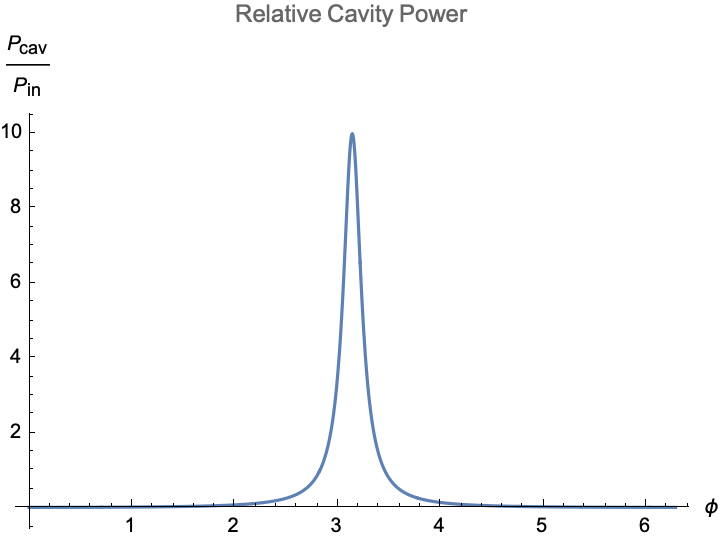
\includegraphics{Exercise7.15.png}
    \end{center}
    We see a sharp peak corresponding to a phase shift of $\pi$. It's clear from equation~\eqref{eq:7.15} that the height of this peak should be $(1-R)^{-1}$. This plot suggests, in order to get large field strengths in the cavity, we should set up our system so that the phase shift is $\pi$ and the reflectivity $R$ is as large as reasonable.

\section{Exercise 7.16 (Electric dipole selection rules)}
    Show that (7.60) is non-zero only when $m_2 - m_1 = \pm 1$ and $\Delta l = \pm 1$.

    \textbf{Solution (Incomplete):} The formulas for the spherical harmonics $Y_{lm}$ appear complicated, but that is in large part due to the normalization factors. Since we are only interested in whether the expectation value is zero, we can ignore them. Even better, the integral $\int d\Omega = \int d\varphi \int \sin\theta d\theta$ factorizes into two parts because the $Y$ are products of functions $P_{lm}(\cos\theta)$ and $e^{im\varphi}$ of each of the variables alone. Thus, the thing we need to check under what circumstances the product
    \begin{align}
        \left(\int_0^\pi \sin \theta P_{1m}(\cos\theta) P_{l_1 m_1}(\cos\theta) P_{l_2 m_2}(\cos\theta)d\theta\right) \times \left(\int_0^{2\pi} e^{i(m + m_2 - m_1)}d\varphi\right)
    \end{align}
    is zero, where $m = \pm 1$. We can simplify the first integral with the variable substitution $x = \cos\theta$.
    \begin{align}
        \left(\int_{-1}^1  P_{1m}(x) P_{l_1 m_1}(x) P_{l_2 m_2}(x)dx\right) \times \left(\int_0^{2\pi} e^{i(m + m_2 - m_1)}d\varphi\right)
    \end{align}
    Of course, the product above is nonzero exactly when each term is nonzero. Let's start with the integral over $\varphi$ because it's simpler. If $m +m_2 - m_1 \neq 0 $, the integral will vanish because we are taking integrals of sine and cosine over its period of $2\pi$. Thus, the integral is nonzero exactly when
    \begin{align}
    \begin{aligned}
        m + m_2 - m_1 &= 0 \\
        m_2 - m_1 &= \pm 1.
    \end{aligned}
    \end{align}

    This answers one part of the question. For the other, let's examine the integral over the associated Legendre polynomials. Writing out the definitions, this is zero exactly when
    \begin{align}
        \int_{-1}^1(1-x^2)^{(m_1 + m_2 + m)/2}\left(\frac{d^{m+1}}{dx^{m+1}}(x^2 - 1)\right)\left(\frac{d^{m_1+l_1}}{dx^{m_1+l_1}}(x^2 - 1)^{l_1}\right)\left(\frac{d^{m_2+l_2}}{dx^{m_2+l_2}}(x^2 - 1)^{l_2}\right) dx
    \end{align}
    is zero. First, let's observe that $m_1 + m_2 + m = 2 m_1$, from our result above, so this becomes
    \begin{align}
        \int_{-1}^1 (1-x^2)^{m_1} \left(\frac{d^{m+1}}{dx^{m+1}}(x^2 - 1)\right)\left(\frac{d^{m_1+l_1}}{dx^{m_1+l_1}}(x^2 - 1)^{l_1}\right)\left(\frac{d^{m_2+l_2}}{dx^{m_2+l_2}}(x^2 - 1)^{l_2}\right)
    \end{align}
    
    One way that these integrals could be zero is that the order of the derivatives are higher than the degree of the polynomial. So we need $m_i + l_i \leq 2l_1$, or \textbf{Incomplete}


\section*{Exercise 7.17 (Eigenstates of the Jaynes-Cummings Hamiltonian)}
    Show that 
    \begin{align}
        \ket{\chi_n} = \frac{1}{\sqrt{2}}\left[\ket{n,1} + \ket{n+1,0}\right] \\
        \ket{\overline{\chi}_n} = \frac{1}{\sqrt{2}}\left[\ket{n,1} - \ket{n+1,0}\right]
    \end{align}
    are eigenstates of the Jaynes-Cummings Hamiltonian (7.71) for $\omega = \delta = 0$, with the eigenvalues
    \begin{align}
        H \ket{\chi_n} &= g\sqrt{n+1} \ket{\chi_n} \\
        H\ket{\overline{\chi}_n} &= -g\sqrt{n+1}\ket{\overline{\chi}_n},
    \end{align}
    where the labels in the ket are $\ket{\text{field}, \text{atom}}$.

    \textbf{Solution}: \underline{Aside on confusing notation} As pointed out in the text, the observable $N$ corresponding to the ``number of excitations" (photons + qubit) commutes with the Hamiltonian. However, there is something we need to be careful about. Unintuitively, the state $\ket{0}$ corresponds to an \emph{excited} qubit, while the state $\ket{1}$ corresponds to a \emph{lack} of excitation. Thus, in some ways, the $\ket{0}$ computational state should really be labelled $\ket{1}$, meaning 1 excitation. To put it another way, the state $\ket{0}$ has $1$ energy quanta, while $\ket{1}$ has $0$ energy quanta. In the context of this problem, the qubit state lables should probably be swapped. 

    To really hammer this point away, notice how the spin excitation operators $\sigma_\pm$ act on the computational basis.
    \begin{align}
        \sigma_+ \ket{0} = 0, \qquad \sigma_+ \ket{1} = \ket{0}.
    \end{align}
    Thus, it looks like $\sigma_+$ is really de-exciting. As a result of these ambiguities, it seems the authors Nielsen and Chuang have made a small error. We can see that $\ket{\chi_n}$ as written isn't really an eigenstate of the Jaynes-Cummings Hamiltonian, assuming they intend for $0,1$ to label computational states and not energy quanta. To see the problem, let's observe that $\ket{n,1}$ and $\ket{n+1, 0}$ are eigenstates of $N$ with \emph{different} eigenvalue.
    \begin{align}
    \begin{aligned}
        N \ket{n,1} &= \left(n - \frac{1}{2}\right) \ket{n,1} \\
        N \ket{n+1, 0} &= \left(n+\frac{3}{2}\right) \ket{n+1,0}
    \end{aligned}
    \end{align}
    Thus, a linear combination of these couldn't produce an eigenstate of $H$, since $H$ and $N$ must share an eigenbasis. 

    Thankfully, with a notational slight of hand, we can fix things. Instead of defining, for example, $\ket{n,0}$ to be $\ket{n}\otimes \ket{0}$, we will adopt the following conventions.
    \begin{align}
        \ket{n,0} \equiv \ket{n}\otimes \ket{1}, \qquad \ket{n,1} \equiv \ket{n}\otimes \ket{0}
    \end{align}
    With this choice, everything should work out correctly, and we will proceed from here as normal. \underline{End of aside.}

    We first observe that that $N$ is a twofold-degenerate operator. For each eigenvalue (``number of excitations") there are two states that give rise to that eigenvalue: $\ket{n, 1}$ and $\ket{n + 1, 0}$. This makes sense: to have $n+1$ total excitations, we either place them all in the cavity, or place one in the qubit and $n$ in the cavity. The qubit can only store one excitation.

    As a side note, a special edge case occurs when there are no excitations: $\ket{0,0}$. This is clearly an eigenstate of $H$ with eigenvalue $-\hbar \omega_0/2$, and we will now consider the case where there is at least one excitation.

    Each eigenstate of $H$ must reside in an eigenspace of $N$. Thus, we can express $H$ as a $2\times 2$ matrix in the eigenbasis $\ket{n, 1}$ and $\ket{n + 1, 0}$. Using equation (7.71), and setting $\omega = \delta = 0$ as the problem asks, we have
    \begin{align}
    \begin{aligned}
        H \ket{n+1,0} &= g \sqrt{n+1} \ket{n, 1} \\
        H\ket{n,1} &= g \sqrt{n+1} \ket{n+1, 0}.
    \end{aligned}
    \end{align}
    In this subspace, we see that $H$ acts essentially like an effective $X$ operation.
    \begin{align}
        H = g\sqrt{n+1}\begin{pmatrix}
            0 & 1 \\
            1 & 0
        \end{pmatrix}
    \end{align}
    Because of this, we can immediately write the eigenstates. 
    \begin{align}
    \begin{aligned}
        \ket{\chi_n} &= \frac{1}{\sqrt{2}}\left(\ket{n, 1} + \ket{n+1,0}\right) \\
        \ket{\overline{\chi}_n} &= \frac{1}{\sqrt{2}}\left(\ket{n, 1} - \ket{n+1,0}\right).
    \end{aligned}
    \end{align}
    This is exactly what we sought to show. The collection of eigenstates is expressible by the set $\{\ket{\chi_n}, \ket{\overline{\chi}_n}\}_n$ for integer $n > 0$, as well as the special case $\ket{\chi_0} = \ket{0,0}$.

    

\section*{Exercise 7.18 (Rabi oscillations)}
    Show that (7.77) is correct by using
    \begin{align}
        e^{i \vec{n}\cdot \vec{\sigma}} = \cos\abs{n} + i \hat{n}\cdot\vec{\sigma} \sin\abs{n}
    \end{align}
    to exponentiate $H$. This is an unusually simple derivation of the Rabi oscillations and the Rabi frequency; ordinarily, one solves coupled differential equations to obtain $\Omega$, but here we obtain the essential dynamics just by focusing on the single-atom, single-photon subspace!

    \textbf{Solution}: There is a small error in the text. Doing a careful analysis of the matrix elements of $H$ in the appropriate subspace, being mindful of the conventions established in Exercise 7.17, one finds that there is a sign error in places. The real $H$ is 
    \begin{align}
        H = \begin{bmatrix}
            -\delta & 0 & 0 \\
            0 & \delta & g \\
            0 & g & -\delta
        \end{bmatrix}.
    \end{align}
    We will therefore start our analysis of $U = e^{-i H t}$ here. 
    
    Given $H$ as above, the first thing we observe is that it is block diagonal. Therefore, to exponentiate $H$, we can exponentiate each block individually. We ignore the overall sign given in equation (7.76), since I believe that is an error.

    Let's label the blocks as $H_1$ and $H_2$, where $H_1$ is the $1\times 1$ upper block and $H_2$ is the $2 \times 2$ lower block. The upper block is easy to exponentiate, and is given by $e^{i\delta t}$. For the lower block, we observe that
    \begin{align}
        H_2 = \delta Z + g X.
    \end{align}
    Hence,
    \begin{align}
        e^{-i H_2 t} = e^{-i \hat{n}\cdot \vec{\sigma} \Omega t}
    \end{align}
    where we've defined $\Omega = \sqrt{g^2 + \delta^2}$ and $\hat{n} = (g, 0 , \delta)/\Omega$. Using the identity given in the problem, we have
    \begin{align}
    \begin{aligned}
        e^{-i \hat{n}\cdot \vec{\sigma}\Omega t} &= \cos{\Omega t} I - i \hat{n}\cdot\vec{\sigma} \sin{\Omega t} \\
        &= \begin{pmatrix}
            \cos\Omega t - i \frac{\delta}{\Omega} \sin\Omega t & -i \frac{g}{\Omega}\sin\Omega t \\
            -i \frac{g}{\Omega}\sin\Omega t & \cos\Omega t + i \frac{\delta}{\Omega}\sin\Omega t.
        \end{pmatrix}
    \end{aligned}
    \end{align}
    
    Having exponentiated each block individually, we can now combine the result.
    \begin{align}
        U = \begin{pmatrix}
            e^{i\delta t} & 0 & 0 \\
            0 & \cos\Omega t - i \frac{\delta}{\Omega} \sin\Omega t & -i \frac{g}{\Omega}\sin\Omega t \\
            0 & -i \frac{g}{\Omega}\sin\Omega t & \cos\Omega t + i \frac{\delta}{\Omega}\sin\Omega t
        \end{pmatrix}.
    \end{align}

    The final step is to convert this to Dirac notation. Noting the ordering of the basis, we have
    \begin{align}
    \begin{aligned}
        U = e^{i\delta t} \ket{00}\bra{00} &+ \left(\cos \Omega t - i \frac{\delta}{\Omega} \sin \Omega t\right) \ket{01}\bra{01} \\
        &+ \left(\cos \Omega t 
        + i \frac{\delta}{\Omega} \sin \Omega t\right) \ket{10}\bra{10} \\
        &-i \frac{g}{\Omega}\sin\Omega t \left(\ket{01}\bra{10} + \ket{10}\bra{01}\right).
    \end{aligned}
    \end{align}
    Notice that the author's answer is slightly different from ours. I believe this is a result of sign errors, but hopefully you (the reader) have enough guidance to figure that out now.
    

\section*{Exercise 7.19 (Lorentzian absorption profile)}
    Plot (7.79) for $t = 1$ and $g = 1.2$, as a function of the detuning $\delta$, and (if you know it) the corresponding classical result. What are the oscillations due to?

    \textbf{Solution}: The plot below gives the plot for these parameters.
    \begin{center}
        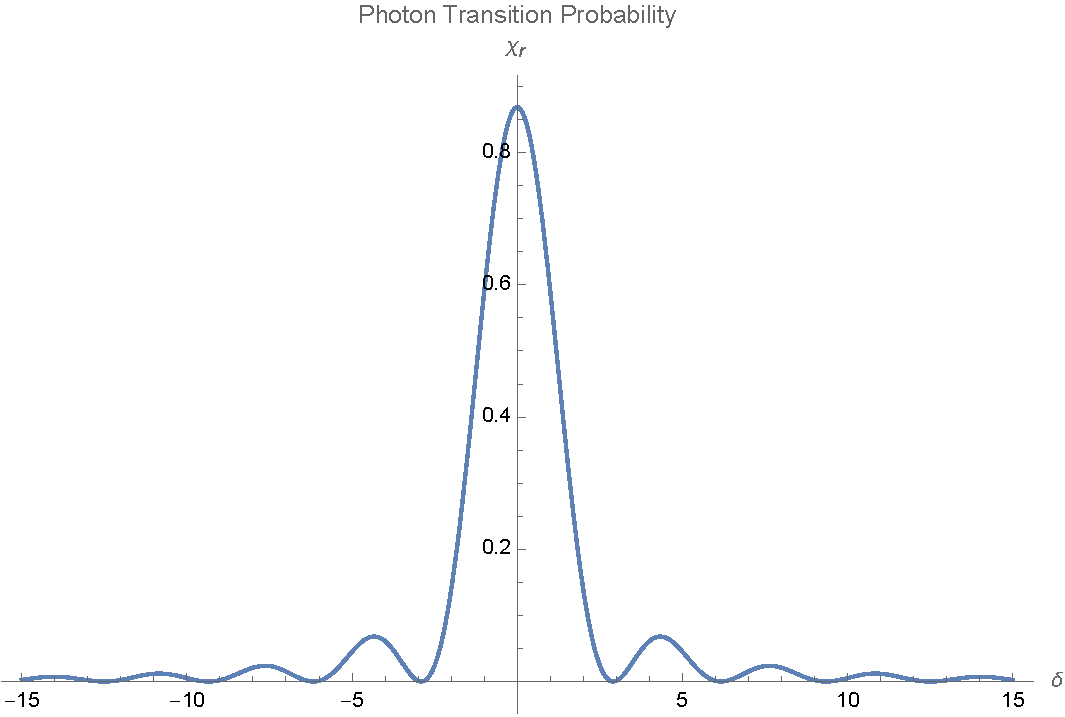
\includegraphics{Exercise7.19.pdf}
    \end{center}
    I produced this directly in Mathematica using the Plot function. Use your favorite choice of plotting software.

    The classical result is essentially the same, without the oscillating factor. The Lorentzian profile in the classical case can be seen to come from the assumption of an exponential decay of a large population of excited atoms. The oscillations are due to the fact that the exchange of excitations really goes both directions. When there is a dip in transition probability, a full cycle of transition occured, where the photon was absorbed and reemitted, perhaps multiple times. 

\section*{Exercise 7.20 (Single photon phase shift)}
    Derive (7.80) from $U$, and plot it for $t = 1$ and $g = 1.2$, as a function of the detuning $\delta$. Compare with $\delta/\Omega^2$.

    \textbf{Solution}:

\section*{Exercise 7.24}
    The energy of a nuclear spin in a magnetic field is approximately $\mu_N B$, where $\mu_N = eh/4\pi m_p \approx 5\times 10^{-27}$ joules per tesla is the nuclear Bohr magneton. Compute the energy of a nuclear spin in a $B=10$ tesla field, and compare with the thermal energy at $k_b T$ at $T = 300 K$.

    \textbf{Solution}: The first part is pretty easy since we are multiplying by 10. The result is $\mu_N B \approx 5 \times 10^{-26}$ joules. On the other hand, the Boltzmann constant $k_B$ has a value of approximately $10^{-23}$ joules per Kelvin. Multplying by 300 kelvin gives $3 \times 10^{-21}$ joules. Comparing the two, we find that $k_B T$ roughly \emph{five orders of magnitude} greater than the nuclear spin energy. 

    This answers the question directly, but let's give a little more context. As far as magnetic fields go, 10 tesla is already quite strong, but within capabilities of modern lab equipment. For reference, as of writing, the strongest steady fields ever produce in a lab are on the order of 32 tesla. We interpret $k_B T$ as roughly the thermal energy available to the system to undergo more-or-less random transitions between energy levels. Since the spin energy is so small compared to this heat energy, we expect the spin to transition ("flip") uncontrollably due to the enormous amounts of energy available. 

    How cold would it have to be to reduce this excess thermal energy to below the nuclear spin energy, thereby suppressing these thermal transitions? Based on our answer, the temperature $T$ would have to be roughly five orders of magnitude lower. This is something like $3 \times 10^{-3}$ K. This is extremely cold, and suggests we will need to use some sophisticated cooling technology, such as a dilution refrigerator, to keep our equipment very cold. Remarkably, such technology currently exists!

\section*{Exercise 7.25}
    Show that the total angular momenta operators obey the commutation relations for $SU(2)$, that is, $[j_i, j_k] = i \epsilon_{ikl} j_l$.

    \textbf{Solution}: We will do this in a more general fashion, without adding too much complications. Imagine we have two systems with angular momenta $\vec{j}^{(1)}$ and $\vec{j}^{(2)}$, respectively. Here the overline arrow on $\vec{j}^{(1)}$ denotes a list of three operators, one for each Cartesian coordinate $x,y,z$. On the joint system, define the operator
    \begin{align} \label{eq:7.25_def}
        \vec{j} \equiv \vec{j}^{(1)} + \vec{j}^{(2)}
    \end{align}
    to be the ``total angular momentum" of the two systems. While this definition seems intuitive ("just add them"), we still need to verify that the three operators in $\vec{j}$ satisfy the commutation relations that essentially define what angular momentum \emph{is} in quantum mechanics. Thus, we need to compute $[j_i, j_k]$. Using the definition~\eqref{eq:7.25_def} and expanding the commutator, we find that
    \begin{align}
        [j_i, j_k] = [j_i^{(1)}, j_k^{(1)}] + [j_i^{(2)}, j_k^{(2)}] + [j_i^{(1)}, j_k^{(2)}] + [j_i^{(2)}, j_k^{(1)}].
    \end{align}
    The last two terms are involve operators acting on different subsystems, and therefore the commutators are zero. On the other hand, we use the fact that $\vec{j}^{(1)}$ and $\vec{j}^{(2)}$ are valid sets of angular momentum operators, so the normal commutation relation holds. Altogether,
    \begin{align}
    \begin{aligned}
        [j_i, j_k] &= i\epsilon_{ikl} j_l^{(1)} + i\epsilon_{ikl} j_l^{(2)} \\
        &= i \epsilon_{ikl}(j_l^{(1)} + j_l^{(2)}) \\
        &= i \epsilon_{ikl}j_l.
    \end{aligned}
    \end{align}
    This gives our result. Comparing with the text, our work specializes to the case of two spin-1/2 particles. 

\section*{Exercise 7.26}
    Verify the properties of $\ket{j, m_j}_J$ by explicity writing the $4\times 4$ matrices $J^2$ and $j_z$ in the basis defined by $\ket{j,m_j}_J$.

    \textbf{Solution}:
    
\chapter{Quantum noise and quantum operations}

\section*{Exercise 8.1 (Unitary evolution as a quantum operation)}
    Pure states evolve under unitary transforms as $\ket{\psi}\rightarrow U\ket{\psi}$. Show that, equivalently, we may write $\rho \rightarrow \mc{E}(\rho) \equiv U \rho U^\dagger$, for $\rho = \ket{\psi}\bra{\psi}$.
    
    \textbf{Solution}: Consider the map $f$ which identifies the ket representation of a pure quantum state, $\ket{\psi}$, with its representation as a rank one density operator.
    \begin{align}
        f(\ket{\psi}) = \ket{\psi}\bra{\psi}
    \end{align}
    Now suppose we have a unitary operation $U$ on the quantum state, which in the ket representation acts as $\ket{\psi}\to U\ket{\psi}$. To arrive at a natural definition of the unitary transformation in the density operator formalism, we can consider what map $\mc{E}$ satisfies the following commutative property.
    \begin{align}
        f(U\ket{\psi}) = \mc{E}(f(\ket{\psi})) = \mc{E}(\ket{\psi}\bra{\psi})
    \end{align}
    Let $\ket{\psi'} = U\ket{\psi}$, so that $f(U\ket{\psi}) = \ket{\psi'}\bra{\psi'}$. I claim that
    \begin{align}
        \ket{\psi'}\bra{\psi'} = U \ket{\psi}\bra{\psi} U^\dagger.
    \end{align}
    To see this, we can show that the right side of this equation sends $\ket{\psi'}$ to itself and anything orthogonal to $\ket{\psi'}$ to the zero vector. Indeed,
    \begin{align}
        U\ket{\psi}\bra{\psi}U^\dagger \ket{\psi'} = U \ket{\psi}\bra{\psi}\ket{\psi} = \bra{\psi}\ket{\psi} U \ket{\psi} = \ket{\psi'}.
    \end{align}
    Similarly, suppose $\ket{\psi'_\perp}$ is orthogonal to $\ket{\psi'}$. Then, $\ket{\psi'_\perp} = U \ket{\psi_\perp}$ for some $\ket{\psi_\perp}$ orthogonal to $\ket{\psi}$. Hence,
    \begin{align}
         U\ket{\psi}\bra{\psi}U^\dagger \ket{\psi'_\perp} = U\ket{\psi}\bra{\psi} \ket{\psi_\perp} = 0.
    \end{align}
    Thus, we see that $\ket{\psi'}\bra{\psi'} = U\ket{\psi}\bra{\psi}U^\dagger$. This demonstrates that the natural definition of a unitary $U$ acting on the density matrix representation of a quantum state is given by
    \begin{align}
        \mc{E}(\ket{\psi}\bra{\psi}) = U\ket{\psi}\bra{\psi}U^\dagger,
    \end{align}
    which is precisely what we sought to show. 
    
\section*{Exercise 8.2} 
    Recall from Section 2.2.3 (on page 84) that a quantum measurement with outcomes labeled by $m$ is described by a set of measurement operators $M_m$ such that $\sum_m M_m^\dagger M_m = I$. Let the state of the system immediately before the measurement be $\rho$. Show that for $\mc{E}_m(\rho) \equiv M_m \rho M_m^\dagger$, the state of the system immediately after the measurement is
    \begin{align} \label{eq:Exercise 8.2 final state}
        \frac{\mc{E}_m(\rho)}{\tr(\mc{E}_m(\rho))}.
    \end{align}
    Also show that the probability of obtaining this measurement result is $p(m) = \tr(\mc{E}_m(\rho))$.
    
    \textbf{Solution}: For reference, the axioms for pure state measurements as provided in the text are as follows. A measurement with outcome $m$ (an event in the probability space) has corresponding probability $p(m)$ and final state $\ket{\psi'}$ given by
    \begin{align} \label{eq:Exercise 8.2 pure state measurement axioms}
    \begin{aligned} 
        p(m) &= \bra{\psi}M_m^\dagger M_m \ket{\psi} \\
        \ket{\psi'} &= \frac{M_m \ket{\psi}}{\sqrt{\bra{\psi}M_m^\dagger M_m \ket{\psi}}},
    \end{aligned}
    \end{align}
    where $\ket{\psi}$ is the initial (pure) state of the system.
    
    The results we are asked to ``show" can be taken as axiomatic for open quantum systems. Unfortunately, because the map \eqref{eq:Exercise 8.2 final state} is not convex linear, we cannot extend the axioms on pure states by linearity. The best we can do is show that \eqref{eq:Exercise 8.2 pure state measurement axioms} imply \eqref{eq:Exercise 8.2 final state} in the case of pure states, then \emph{assert} (i.e. define) the result to hold for any mixed state. This is what we do below.
    
    First, consider the expression $p(m)$ in terms of ket $\ket{\psi}$. We have
    \begin{align}
    \begin{aligned}
        p(m) &= \bra{\psi}M_m^\dagger M_m \ket{\psi} \\
        &= \tr (M_m^\dagger M_m \ket{\psi}\bra{\psi}) \\
        &= \tr (M_m\ket{\psi}\bra{\psi}M_m^\dagger) \\
        &= \tr(\mc{E}_m(\rho)).
    \end{aligned}
    \end{align}
    where we used the property that the trace is cyclic and that, for any operator $A$ and pure state,
    \begin{align}
        \tr( A \ket{\psi}\bra{\psi}) = \bra{\psi}A\ket{\psi}.
    \end{align}
    Now consider the pure state after measurement, which as a density operator is given by $\ket{\psi'}\bra{\psi'}$. Using the transformation given by the second line of \eqref{eq:Exercise 8.2 pure state measurement axioms},
    \begin{align}
        \ket{\psi'}\bra{\psi'} = \frac{M_m\ket{\psi}\bra{\psi}M_m^\dagger}{\bra{\psi} M_m^\dagger M_m\ket{\psi}} = \frac{\mc{E}_m(\ket{\psi}\bra{\psi})}{\tr(\mc{E}_m(\ket{\psi}\bra{\psi}))}.
    \end{align}
    This shows the result for pure state density matrices that we desire. We can now extend this definition to all quantum states, mixed and pure. 
    
\section*{Exercise 8.3}
    Our derivation of the operator-sum representation implicitly assumed that the input and output spaces for the operation were the same. Suppose a composite system $AB$ initially in an unknown quantum state $\rho$ initially in an unknown quantum state $\rho$ is brought into contact with a composite system $CD$ initially in some standard state $\ket{0}$, and the two systems interact according to a unitary interaction $U$. After the interaction we discard systems $A$ and $D$, leaving a state $\rho'$ of the system $BC$. Show that the map $\mc{E}(\rho) = \rho'$ satisfies
    \begin{align}
        \mc{E}(\rho) = \sum_k E_k \rho E_k^\dagger
    \end{align}
    for some set of linear operators $E_k$ from the state space of the system $AB$ to the state space of system $BC$, and such that $\sum_k E_k^\dagger E_k = I$.
    
    \textbf{Solution}: The action of $\mc{E}$ from $AB$ to $BC$ is summarized as follows: append a system $CD$ with state $\ket{0}$, apply a unitary $U$ which acts on the combined system $ABCD$, and trace out system $AD$. More explicitly,
    \begin{align}
        \mc{E}(\rho) = \tr_{AD}(U \rho \otimes \ket{0}\bra{0} U^\dagger).
    \end{align}
    Let $\{\ket{u_k}\}$ form an orthonormal basis for the space of system $AD$. Computing the trace with respect to this basis, we have
    \begin{align} \label{eq:Exercise 8.3}
    \begin{aligned}
        \mc{E}(\rho) &= \sum_k \bra{u_k}U \rho \otimes \ket{0}\bra{0}U^\dagger \ket{u_k} \\
        &= \sum_k \bra{u_k}U\ket{0}\rho \bra{0}U^\dagger \ket{u_k}
    \end{aligned}
    \end{align}
    Note that we can freely move the ket $\ket{0}$ across $\rho$ to match with $U$ since $\rho$ and $\ket{0}$ live in difference spaces. Consider the object $E_k$ defined by
    \begin{align}
        E_k \equiv \bra{u_k}U\ket{0}.
    \end{align}
    This is, in fact, an operator from the space of $AB$ to $BC$. From \eqref{eq:Exercise 8.3} we have
    \begin{align}
        \mc{E}(\rho) = \sum_k E_k \rho E_k^\dagger
    \end{align}
    as desired. Moreover, we can check that the completeness relation is satisfied, as it must be for probability conservation.
    \begin{align}
        \sum_k E_k^\dagger E_k = \sum_k \bra{0}U^\dagger \ket{u_k}\ket{u_k}U\bra{0} = \bra{0}U^\dagger \left(\sum_k \ket{u_k}\bra{u_k}\right) U\ket{0} = \bra{0}U^\dagger U \ket{0} = I_{AB}
    \end{align}
    where the subscript emphasizes the space the identity is acting on. 
    
\section*{Exercise 8.4 (Measurement)}
    Suppose we have a single qubit principal system, interacting with a single qubit environment through the transform
    \begin{align}
        U = P_0\otimes I + P_1 \otimes X
    \end{align}
    where $X$ is the usual Pauli matrix (acting on the environment) and $P_0\equiv \ket{0}\bra{0}$, $P_1 \equiv \ket{1}\bra{1}$ are projectors (acting on the system). Give the quantum operation for this process, in the operator-sum representation, assuming the environment starts in the state $\ket{0}$.
    
    \textbf{Solution}: There will be two operation elements, $E_0$ and $E_1$, since the dimension of the environment is two. Moreover, per the preceding discussion these will be given by
    \begin{align}
        E_j = \bra{u_j}U\ket{0}
    \end{align}
    where the $\ket{u_j}$ form an orthonormal basis for the environment. Let's take these to be the computational basis. We then have
    \begin{align}
    \begin{aligned}
        E_0 = \bra{0}U\ket{0} = P_0\otimes \bra{0}I\ket{0} + P_1 \otimes \bra{0}X\ket{0} = P_0 \\
        E_1 = \bra{1}U\ket{0} = P_0\otimes \bra{1}I\ket{0} + P_1 \otimes \bra{1}X\ket{0} = P_1.
    \end{aligned}
    \end{align}
    Thus, the quantum operation $\mc{E}$ can be expressed as
    \begin{align}
        \mc{E}(\rho) = P_0 \rho P_0 + P_1 \rho P_1
    \end{align}
    Note that this is equivalent to a measurement in the computational basis. It is straightforward to show that these operators satisfy the completeness relation. 

\section*{Exercise 8.5 (Spin flips)}
    Just as in the previous exercise, but now let 
    \begin{align}
        U = \frac{X}{\sqrt{2}}\otimes I + \frac{Y}{\sqrt{2}}\otimes X.
    \end{align}
    Give the quantum operation for this process, in the operator-sum representation.
    
    \textbf{Solution}: We compute the Kraus operators as above, and get the following results.
    \begin{align}
        E_0 = \bra{0}U\ket{0} = \frac{X}{\sqrt{2}} \\
        E_1 = \bra{1}U\ket{0} = \frac{Y}{\sqrt{2}}
    \end{align}
    Note that the $E_0$ corresponds to a spin flip, while $E_1$ corresponds to a spin flip followed by phase flip. We can interpret each event occurring with probability $\frac{1}{2}$.
    
\section*{Exercise 8.6 (Composition of quantum operations)}
    Suppose $\mc{E}$ and $\mc{F}$ are quantum operations on the same quantum system. Show that the composition $\mc{F}\circ \mc{E}$ is a quantum operation, in the sense that it has an operator-sum representation. State and prove an extension of this result to the case where $\mc{E}$ and $\mc{F}$ do not necessarily have the same input and output spaces. 
    
    \textbf{Solution}: Let $\{E_i\}$ and $\{F_j\}$ be the operation elements for the channels $\mc{E}$ and $\mc{F}$ respectively. Considering the action of the composition $\mc{F} \circ \mc{E}$ on an arbitrary input state $\rho$.
    \begin{align}
    \begin{aligned}
        \mc{F}\circ\mc{E} (\rho) &= \mc{F}(\mc{E}(\rho)) \\
        &= \sum_j F_j \mc{E}(\rho) F_j^\dagger \\
        &= \sum_j F_j \left(\sum_i E_i \rho E_i^\dagger \right) F_j^\dagger \\
        &= \sum_{ji} F_j E_i \rho E_i^\dagger F_j^\dagger \\
        &= \sum_{ji} G_{ji} \rho G_{ji}^\dagger 
    \end{aligned}
    \end{align}
    where $G_{ji} \equiv F_j E_i$ is the composition of the two operation elements. Note that this derivation holds as long as the output space of $\mc{E}$ matches the input space of $\mc{F}$, as is required for the composition to be well-defined anyways. One can check that the completeness relation
    \begin{align}
        \sum_{ji}G_{ji}^\dagger G_{ji} \leq I 
    \end{align}
    is satisfied.

\chapter{Distance measures for quantum information}

\section*{Exercise 9.1}
    What is the trace distance between the probability distribution (1, 0) and the probability distribution (1/2, 1/2)? Between (1/2, 1/3, 1/6) and (3/4, 1/8, 1/8)?
    
    \textbf{Solution}: Let's apply the definition in each case.
    \begin{align}
    \begin{aligned}
        D((1,0), (1/2,1/2)) &= \frac{1}{2} (\abs{1-1/2}+\abs{0-1/2}) = \frac{1}{2}\\
        D((1/2,1/3,1/6), (3/4,1/8,1/8)) &= \frac{1}{2} (\abs{1/4} + \abs{5/24}+\abs{1/24}) = \frac{1}{4}
    \end{aligned}
    \end{align}
    
\section*{Exercise 9.2}
    Show that the trace distance between probability distributions $(p, 1 - p)$ and $(q, 1 - q)$ is $\abs{p - q}$.
    
    \textbf{Solution}: Again applying the definition,
    \begin{align}
    \begin{aligned}
        D((q,1-q), (p,1-p)) &= \frac{1}{2}(\abs{q-p} + \abs{(1-q)-(1-p)}) \\
        &= \frac{1}{2} (2 \abs{p-q}) \\
        &= \abs{p-q}
    \end{aligned}
    \end{align}

\section*{Exercise 9.3}
    What is the fidelity of the probability distributions (1, 0) and (1/2, 1/2)? Of (1/2, 1/3, 1/6) and (3/4, 1/8, 1/8)?
    
    \textbf{Solution}: Let's once again apply the definition of fidelity to these distributions.
    
    \begin{align}
    \begin{aligned}
        F((1,0),(1/2,1/2)) &= 1\times \sqrt{1/2} + 0 = \frac{1}{\sqrt{2}} \\
        F((1/2,1/3,1/6),(3/4,1/8,1/8)) &= \sqrt{1/2\times 3/4} + \sqrt{1/3\times 1/8}+\sqrt{1/6\times 1/8} \\
        &= \frac{1}{2}(\sqrt{3/2} + 1/\sqrt{6}+1/(2\sqrt{3}))
        &\approx 0.96
    \end{aligned}
    \end{align}

\section*{Exercise 9.4}
    Prove (9.3).
    
    \textbf{Solution}: Let $X$ be the index set for the outcomes $x$. Note that we may write
    \begin{align} \label{eq:Exercise_9.4_1}
        \frac{1}{2}\sum_{x\in X} \abs{p_x-q_x} = \frac{1}{2}\sum_{x\in P} (p_x-q_x) + \frac{1}{2} \sum_{x\notin P} (q_x-p_x)
    \end{align}
    where $P = \{x\in X| p_x \geq q_x\}$. This amounts to breaking up the absolute value depending on the sign of $p_x-q_x$. I claim that both sums on the right side of the equation are, in fact, equal. This follows from normalization of probabilities, which in this case can be cast as 
    \begin{align}
        \sum_{x\notin P} p_x = 1-\sum_{x\in P} p_x
    \end{align}
    and similar for $q_x$. Thus,
    \begin{align}
        \sum_{x\notin P} (q_x-p_x) = (1-\sum_{x\in P}q_x) - (1-\sum_{x\in P}p_x) = \sum_{x\in P }(p_x - q_x).
    \end{align}
    Applying this relationship to equation \eqref{eq:Exercise_9.4_1} gives
    \begin{align}
        D(p_x, q_x) = \frac{1}{2}\sum_{x\in X} \abs{p_x-q_x} = \sum_{x\in P} p_x - q_x.
    \end{align}
    We could have just as well summed over $Q = X\setminus P$ and gotten the same result, provided we summed over $q_x-p_x$ instead. 
    
    Let's now argue that $P$ is the set that maximizes the sum, that is,
    \begin{align} \label{eq:Exercise_9.4_2}
        \sum_{x\in P } (p_x-q_x) = \max_{S\subset X} \sum_{x\in S} (p_x -q_x).
    \end{align}
    To see this, note that $P$ contains every element $x$ such that $p_x-q_x$ is positive (or zero, though this doesn't matter in terms of the sum), and doesn't contain elements for which it is negative. Thus, elements of $P$ only increase the sum, never decrease. And $P$ contains all such positive elements. This means that equation \eqref{eq:Exercise_9.4_2} holds. Since the left hand side equals the trace distance, we have our result. The only thing that remains is to argue that the equality remains unchanged when we include the absolute value sign; this will be done in the subsequent exercise. 
    
\section*{Exercise 9.5}
    Show that the absolute value signs may be removed from Equation (9.3), that is,
    \begin{align}
        D(p_x, q_x) = \max_s (p(S)-q(S)) = \max_S \left(\sum_{x\in S} p_x -\sum_{x\in S} q_x\right).
    \end{align}
    
    \textbf{Solution}: To maximize the absolute value, we can either sum over all the $x$ where $p_x-q_x$ is positive, or those in which it is negative, and take the maximum of these two with absolute value. However, because of the normalization of probability to one, these two are equal anyways, as I argue in the previous exercise as an intermediate step. Hence, we can always just choose the positive sum, so the absolute value sign is not necessary. 
    
\section*{Exercise 9.6}
    What is the trace distrance between the density operators
    \begin{align}
        \frac{3}{4}\ket{0}\bra{0}+\frac{1}{4}\ket{1}\bra{1};\quad \frac{2}{3}\ket{0}\bra{0}+\frac{1}{3}\ket{1}\bra{1}?
    \end{align}
    Between:
    \begin{align}
        \frac{3}{4}\ket{0}\bra{0}+\frac{1}{4}\ket{1}\bra{1};\quad \frac{2}{3}\ket{+}\bra{+}+\frac{1}{3}\ket{-}\bra{-}?
    \end{align}
    (Recall that $\ket{\pm} = (\ket{0}\pm\ket{1})/\sqrt{2}.)$
    
    \textbf{Solution}: (Example 1) This example is relatively simple, since both operators are already diagonal in the computational basis. We basically just need the difference, absolute valued, of the diagonal elements. Here is the full computation.
    \begin{align}
    \begin{aligned}
         &\frac{1}{2}\left(\abs{\frac{3}{4}-\frac{2}{3}}+\abs{\frac{1}{4}-\frac{1}{3}}\right) \\
         &= \frac{1}{2}\left(\frac{1}{12}+\frac{1}{12}\right) \\
         &= \frac{1}{12}
    \end{aligned}
    \end{align}
    
    (Example 2) This one is a bit trickier, because the two operators under consideration do not commute. To proceed, we will calculate the eigenvalues of the difference. Let $\rho$ and $\sigma$ denote the first and second density operators, respectively. We will diagonalize the difference $\rho-\sigma$, and it will be helpful to express everything as a matrix in the computational basis. These are given by
    \begin{align}
        \rho =
        \begin{pmatrix}
            3/4 & 0 \\
            0 & 1/4
        \end{pmatrix} \quad 
        \sigma = 
        \begin{pmatrix}
            1/2 & 1/6 \\
            1/6 & 1/2
        \end{pmatrix}.
    \end{align}
    It's a good idea to do the computation for $\sigma$ yourself. Note that the matrix forms are symmetric and have trace 1, as expected. They are also positive definite. None of this should be surprising, of course. The difference $\rho - \sigma$ is then given by 
    \begin{align}
        \rho-\sigma = 
        \begin{pmatrix}
            1/4 & -1/6 \\
            -1/6 & -1/4
        \end{pmatrix}.
    \end{align}
    Now we compute the eigenvalues. Do this using your favorite method. The two eigenvalues, $\lambda_+$, $\lambda_-$ are given by
    \begin{align}
        \lambda_\pm = \pm \frac{\sqrt{13}}{12}
    \end{align}
    Thus, taking the sum of the absolute values, and dividing by two, we get the trace distance: $\sqrt{13}/12$. Again, it's a good idea to check this. 
    
\section*{Exercise 9.7}
    Show that for any states $\rho$ and $\sigma$, one may write $\rho-\sigma = Q-S$, where $Q$ and $S$ are positive operators with support on orthogonal vector spaces. (Hint: use the spectral decomposition $\rho -\sigma = U DU^\dagger$, and split the diagonal matrix $D$ into positive and negative parts. This fact will continue to be useful later.)
    
    \textbf{Solution}: Though we are proving this for the specific case $\rho -\sigma$, with two quantum states, this is really quite more general. All we require is the difference $\rho - \sigma$ be Hermitian, which it certainly is in this case. Any Hermitian operator can be diagonalized, and one way to understand this is to say that $\rho - \sigma$ may be expressed as a combination of orthogonal projectors.
    \begin{align} \label{eq:Exercise_9.7}
        \rho - \sigma = \sum_j \lambda_j \ket{\lambda_j}\bra{\lambda_j}
    \end{align}
    Here, the sum is taken over all (nonzero) eigenvalues $\lambda_j$, with corresponding eigenvector $\ket{\lambda_j}$ (in case of multiplicity, $\lambda_j$ may be equal to $\lambda_k$ for $j\neq k$. However, in this case we can make a choice so that $\ket{\lambda_j}$ and $\ket{\lambda_k}$ are orthogonal. The notation is tricky but useful). Let us reorganize the sum into two pieces, one in which the eigenvalues are positive, and one containing the remaining, negative terms. Call these terms $Q$ and $T$, respectively. Clearly, $Q$ is positive; its eigenvalues are either zero or $\lambda_j$ for positive $\lambda_j$. Moreover, $T$ is clearly negative, since all it's eigenvalues are negative or zero. Thus, $S = -T$ is positive. Moreover, by construction, we have
    \begin{align}
        \rho - \sigma = Q + T = Q - S
    \end{align}
    The fact that $Q$ and $S$ act on orthogonal subspaces is also a consequence of the hermiticity of $\rho -\sigma$, which implies that all the eigenvectors in equation \eqref{eq:Exercise_9.7} are mutually orthogonal.

\section*{Exercise 9.8 (Convexity of the trace distance)} 
    Show that the trace distance is convex in its first input,
    \begin{align}
        D\left(\sum_i p_i\rho_i, \sigma\right) \leq \sum_i p_i D(\rho_i, \sigma).
    \end{align}
    By symmetry convexity in the second entry follows from convexity in the first.
    
    \textbf{Solution}: We would like to somehow take advantage of the joint convexity result, which seems like it should directly imply the result we seek. To make it work in our favor, we can employ a trick: write $\sigma = \sum_i p_i \sigma_i$, where $\sigma_i = \sigma$ for all $i$. Now, $\sigma$ is written so that we can apply joint convexity. As a final step, simply replace $\sigma_i = \sigma$ in the resulting formula. This will prove the result. 
    
\section*{Exercise 9.9 (Existence of fixed points)} 
    \emph{Schauder's fixed point theorem} is a classic result from mathematics that implies that any continuous map on a convex, compact subset of a Hilbert space has a fixed point. Use Schauder’s fixed point theorem to prove that any trace-preserving quantum operation $\mc{E}$ has a fixed point, that is, $\rho$ such that $\mc{E}(\rho) = \rho$. 
    
    \textbf{Solution}: We simply need to show that a trace-preserving quantum operation $\mc{E}$ satisfies the criteria of the theorem. First, note that the collection of self-adjoint operators on a complex Hilbert space is \emph{itself} a real Hilbert space, with inner product defined by $\langle A, B \rangle \equiv \tr(A B)$. Quantum operations are maps on the set of density operators, which are a subset of this Hilbert space of operators. And we know this map is continuous, since, after all, the map $\mc{E}$ is contractive with respect to trace distance, and therefore keeps quantum states close together (this could probably be demonstrated more rigorously). Therefore, we need to check that this set $\mc{D}$ of density operators is convex and compact. We already know $\mc{D}$ is convex: any convex combination of states $\rho$ and $\sigma$, 
    \begin{align}
        \lambda \rho + (1-\lambda) \sigma,
    \end{align} is itself a valid state. To prove compactness, we will take advantage of the so-called \emph{Heine-Borel theorem}, which says that subset of a space which is the "same as" an n-dimensional real space, $\mathbb{R}^n$ is compact if and only it is closed and bounded. Bound just means the set doesn't extend indefinitely. Closed means there is some boundary that lies within the set. Both these properties can be understood, in our circumstances, as a consequence of the existence of pure states, which are \emph{extremal points} of $\mc{D}$. This means pure states form the boundary for density operators, and of course this boundary is included in $\mc{D}$. All of this can be proved with greater rigor, but hopefully this gives a starting point for understanding the result. With these properties in hand, we can use the Schauder theorem to assert a map $\mc{E}$ on $\mc{D}$ has at least one fixed point $\rho \in \mc{D}$.
    
\section*{Exercise 9.10}
    Suppose E is a \emph{strictly contractive} trace-preserving quantum operation, that is, for any $\rho$ and $\sigma$, $D(\mc{E}(\rho), \mc{E}(\sigma)) < D(\rho, \sigma)$. Show that E has a unique fixed point.
    
    \textbf{Solution}: From the previous exercise, we know that $\mc{E}$ has at least one fixed point. Let $\rho$ and $\sigma$ be fixed points, possibly equal. We will show that, in fact, it must be that $\rho = \sigma$. By definition of fixed point, the states are invariant under the map: $\mc{E}(\rho) = \rho$ and $\mc{E}(\sigma) = \sigma$. Therefore, $D(\mc{E}(\rho),\mc{E}(\sigma)) = D(\rho, \sigma)$. On the other hand, because $D$ is strictly contractive, $D(\mc{E}(\rho), \mc{E}(\sigma)) \leq D(\rho, \sigma)$, with equality if and only if $\rho = \sigma$. Since we indeed have equality, it must be that $\rho = \sigma$. Thus, every fixed point of $\mc{E}$ is the same, and therefore unique.

\section*{Exercise 9.11}
    Suppose $\mc{E}$ is a trace-preserving quantum operation for which there exists a density operator $\rho_0$ and a trace-preserving quantum operation $\mc{E}'$ such that
    \begin{align}
        \mc{E}(\rho) = p\rho_0 + (1-p)\mc{E}'(\rho)
    \end{align}
    for some $p, 0 < p \leq 1$. Physically, this means that with probability $p$ the input state is thrown out and replaced with the fixed state $\rho_0$, while with probability $1 - p$ the operation $\mc{E}'$ occurs. Use joint convexity to show that $\mc{E}$ is a strictly contractive quantum operation, and thus has a unique fixed point.
    
    \textbf{Solution}: Let $\rho$ and $\sigma$ be distinct quantum states, and consider the distance between the states after application of the operation $\mc{E}$.
    \begin{align}
        D(\mc{E}(\rho),\mc{E}(\sigma)) = D(p\rho_0 + (1-p)\mc{E}'(\rho), p \rho_0 + (1-p)\mc{E}'(\sigma))
    \end{align}
    Using the joint convexity of the trace distance,
    \begin{align}
    \begin{aligned}
        D(\mc{E}(\rho),\mc{E}(\sigma)) &\leq p D(\rho_0, \rho_0) + (1-p)D(\mc{E}'(\rho) \mc{E}'(\sigma)) \\
        &= (1-p) D(\mc{E}'(\rho), \mc{E}'(\sigma)) \\
        &< D(\mc{E}'(\rho), \mc{E}'(\sigma))\\
        &\leq D(\rho, \sigma)
    \end{aligned}
    \end{align}
    In the process we used the fact that $1-p <1$ and that any quantum channel, particularly $\mc{E}'$, is contractive. From this string of inequalities, one of which is strict, we can conclude that $D(\mc{E}(\rho), \mc{E}(\sigma)) < D(\rho, \sigma)$, hence the map is strictly contractive. By the results of the previous exercise, it also has a unique fixed point. 
    
\section*{Exercise 9.12}
    Consider the depolarizing channel introduced in Section 8.3.4 on page 378, $\mc{E}(\rho) = pI/2 + (1 - p)\rho$. For arbitrary $\rho$ and $\sigma$ find $D(\mc{E}(\rho), \mc{E}(\sigma))$ using the Bloch representation, and prove explicitly that the map $\mc{E}$ is strictly contractive, that is, $D(\mc{E}(\rho), \mc{E}(\sigma)) < D(\rho, \sigma)$.
    
    \textbf{Solution}: Note that the depolarizing channel meets the criteria of the map $\mc{E}$ of the previous exercise, and therefore we could conclude right away that the map is strictly contractive. However, as the problem suggests, we will show this explicitly in the Bloch representation, which will serve as a nice illustration. Recall that any qubit state $\rho$ can be parametrized as 
    \begin{align}
        \rho = \frac{1}{2}(I+\Vec{r}\cdot\vec{\sigma})
    \end{align}
    where $\norm{\vec{r}} \leq 1$. The 3-vector $\vec{r}$ gives the location of the state in the Bloch ball. The action of the depolarizing channel $\mc{E}$ can be expressed solely in terms of changing $\vec{r}$, and we can compute this action.
    \begin{align}
    \begin{aligned}
        \mc{E}(\rho) &= pI/2 + (1-p)\frac{1}{2}(I+\vec{r}\cdot\vec{\sigma}) \\
        &= I/2 + \frac{1-p}{2}\vec{r}\cdot\vec{\sigma}\\
        &= \frac{1}{2}(I+\vec{r}'\cdot\vec{\sigma})
    \end{aligned}
    \end{align}
    where $\vec{r}' = (1-p) \vec{r}$. Hence, the depolarizing channel shrinks any Bloch vector by the factor $1-p<1$. From this geometric, picture, it should be clear that this map is strictly contractive: all quantum states get closer together after application of the map. Indeed, the trace distance for qubits is directly proportional to the Euclidean distance of the corresponding Bloch vectors. This proves our result. 
    
\section*{Exercise 9.13}
    Show that the bit flip channel (Section 8.3.3) is contractive but not strictly contractive. Find the set of fixed points for the bit flip channel.
    
    \textbf{Solution}: We showed in Exercise 9.10 that all strictly contractive quantum operations have unique fixed points. Therefore, by the contrapositive, if an operation \emph{does} have multiple fixed points, it cannot be strictly contractive. Since every quantum operation is contractive by Theorem 9.2, we simply need to show there are multiple fixed points. Recall that the bit flip channel $\mc{E}$ is defined by
    \begin{align}
        \mc{E}(\rho) = p X\rho X + (1-p) \rho.
    \end{align}
    Let us find the set of points $\rho$ such that $\mc{E}(\rho) = \rho$. Applying the definition and simplifying,
    \begin{align}
        p X\rho X +(1-p)\rho = \rho \quad \Leftrightarrow \quad X \rho X = \rho.
    \end{align}
    In turn, this is equivalent to
    \begin{align}
        [\rho, X] = 0.
    \end{align}
    Hence, any state which commutes with pauli $X$ is unchanged by the channel. This makes sense intuitively, since these states are eigenstates of the pauli $X$ operator. These states can be understood as the set of all Bloch vectors lying along the x-axis. Clearly there are many (in fact, infinite) such states. Therefore, $\mc{E}$ is not strictly contractive.
    
\section*{Exercise 9.14 (Invariance of fidelity under unitary transformations)}
    Prove (9.61) by using the fact that for any positive operator $A$, $\sqrt{UAU^\dagger} = U\sqrt{A}U^\dagger$.
    
    \textbf{Solution}: Let $\rho' = U \rho U^\dagger$ and similarly for $\sigma$. Making use of the square root property given in the problem, we have
    \begin{align}
        \rho'^{1/2}\sigma'\rho'^{1/2} = (U\rho^{1/2} U^\dagger) (U \sigma U^\dagger) (U\rho^{1/2}U^\dagger) = U \rho^{1/2}\sigma\rho^{1/2}U^\dagger.
    \end{align}
    This is the type of isomorphism property we expect matrices to respect under multiplication. Because of this, we have
    \begin{align}
    \begin{aligned}
        F(\rho', \sigma') &= \tr\sqrt{U\rho^{1/2}\sigma\rho^{1/2}U^\dagger} \\
        &= \tr U \sqrt{\rho^{1/2}\sigma\rho^{1/2}} U^\dagger \\
        &= \tr \sqrt{\rho^{1/2}\sigma\rho^{1/2}} \\
        &= F(\rho, \sigma).
    \end{aligned}
    \end{align}
    Along the way, we again used the square root property for positive operators, as well as the cyclic property of the trace. This completes the proof.
    
\section*{Exercise 9.15}
    Show that
    \begin{align}
        F(\rho, \sigma) = \max_{\ket{\varphi}} \abs{\bra{\psi}\ket{\varphi}}
    \end{align}
    where $\ket{\psi}$ is any fixed purification of $\rho$, and the maximization is over all purifications of $\sigma$.
    
    \textbf{Solution}: Let's return to an earlier line of the derivation for the full proof of Uhlmann's theorem. At equation (9.70) of the text, we showed that for any purifications $\ket{\psi}$ and $\ket{\varphi}$ of $\rho$ and $\sigma$ respectively,
    \begin{align}
        \abs{\bra{\psi}\ket{\varphi}} = \abs{\tr(\sqrt{\rho}\sqrt{\sigma}U)},
    \end{align}
    where $U = V_Q V_R^\dagger U_R U_Q^\dagger$. As in the original derivation, let $V$ be the unitary part of the polar decomposition of $\sqrt{\rho}\sqrt{\sigma}$.
    \begin{align}
        \sqrt{\rho}\sqrt{\sigma} = \abs{\sqrt{\rho}\sqrt{\sigma}} V.
    \end{align}
    As before, we need to set $VU=I$ in order to achieve the maximum value and match the fidelity. But this time we can only change $V_Q$ and $V_R$, not $U_Q$ and $U_R$ (which are fixed by our choice of purification of $\ket{\psi}$). Thankfully, we can still accomplish this. Set $V_R = U_R$ and $V_Q = V^\dagger U_Q$. Then,
    \begin{align}
        VU = V V_Q V_R^\dagger U_R U_Q^\dagger = V V^\dagger U_Q U_R^\dagger U_R U_Q^\dagger = I.
    \end{align}
    This completes the proof: we only need to maximize one of the two purifications.
    
\section*{Exercise 9.16}
    Suppose $R$ and $Q$ are two quantum systems with the same Hilbert space. Let $\ket{i_R}$ and $\ket{i_Q}$ be orthonormal basis sets for $R$ and $Q$. Let $A$ be an operator on $R$ and $B$ an operator on $Q$. Define $\ket{m} \equiv \sum_i \ket{i_R}\ket{i_Q}$. Show that
    \begin{align}
        \tr(A^\dagger B) = \bra{m} A \otimes B \ket{m}
    \end{align}
    where the multiplication on the left hand side is of matrices, and it is understood that the matrix elements of $A$ are taken with respect to the basis $\ket{i_R}$ and those for $B$ with respect to the basis $\ket{i_Q}$.
    
    \textbf{Solution}: Let's explicitly evaluate the right side of the equation. We have
    \begin{align}
    \begin{aligned}
        \bra{m} A \otimes B \ket{m} &= \sum_{i} \bra{i_R}\bra{i_Q} A \otimes B \sum_j \ket{j_R}\ket{j_Q} \\
        &= \sum_{ij} \bra{i_R}A\ket{j_R} \bra{i_Q}B\ket{j_Q} \\
        &= \sum_{ij} A_{ij} B_{ij} 
    \end{aligned}
    \end{align}
    where $A_{ij} \equiv \bra{i_R}A\ket{j_R}$ are the matrix elements with respect to the basis, as are $B_{ij}$. 

    This is quite an interesting result, because we can view $\vert m \rangle$ as a maximally entangled ("Bell") state. Apparently, the expectation value of $A \otimes B$ with respect to this entangled state computes the inner  product between $A$ and $B$. 

\section*{Exercise 9.17}
    Show that $0 \leq A(\rho, \sigma) \leq \pi/2$, with equality in the first inequality if and only if $\rho = \sigma$.

    \textbf{Solution}: To define the inverse of $\cos$, which is $\arccos$, we must choose a particular interval of angles $\theta$ on which $\cos(\theta)$ is invertible. A reasonable (and standard) choice is to take angles $\theta \in [0,\pi]$. With this choice, the $\arccos$ function has a domain $[-1,1]$ (corresponding to the range of cosine) and a range from $[0,\pi]$.

    In our present case, we are looking at $\arccos F(\rho, \sigma)$, with $F(\rho, \sigma) \in [0,1]$. The question is, for $x$ between 0 and 1, what is $\arccos(x)$? To determine this, we note that, for the angles $\theta \in [0,\pi]$ that we are interested in, $\cos \theta$ is nonnegative only in the first quadrant (including the axes themselves). These angles are precisely the interval $[0,\pi/2]$. This implies that the image of the interval $\arccos ([0,1])$ of the unit inverval under $arccos$ is  $[0,\pi/2]$. Hence $A(\rho, \sigma) \in [0,\pi/2]$. 

    When does $A(\rho, \sigma) = 0$? Exactly when $\arccos(x) = 0$, where $x = F(\rho, \sigma)$. This occurs when $x = \cos\theta = 1$, meaning $F(\rho, \sigma) = 1$. We've already seen that this is equivalent to $\rho = \sigma$. Hence, $A(\rho, \sigma) = 0$ exactly when $\rho = \sigma$.

\section*{Exercise 9.18 (Contractivity of the angle)}
    Let $\mc{E}$ be a trace-preserving quantum operation. Show that
    \begin{align}
        A(\mc{E}(\rho), \mc{E}(\sigma)) \leq A(\rho, \sigma).
    \end{align}

    \textbf{Solution}: This follows directly from the fact that $F$ is monotonic, while $\arccos$ is monotonically decreasing on $[0,1]$ (with range $[0,\pi/2]$). In more detail we have that $\arccos(y) \leq \arccos(x)$ whenever $y \geq x$. In our case we have
    \begin{align}
        F(\mc{E}(\rho), \mc{E}(\sigma)) \geq F(\rho, \sigma).
    \end{align}
    Hence,
    \begin{align}
        \arccos F(\mc{E}(\rho), \mc{E}(\sigma)) \leq \arccos F(\rho, \sigma).
    \end{align}
    which implies the result by definition of $A$.

\section*{Exercise 9.19 (Joint concavity of fidelity)}
    Prove that the fidelity is \emph{jointly concave},
    \begin{align}
        F\left(\sum_i p_i \rho_i, \sum_i, p_i \sigma_i \right) \geq \sum_i p_i F(\rho_i, \sigma_i).
    \end{align}

    \textbf{Solution}: This follows directly from strong concavity, as given in Theorem 9.7 of the text. In particular, let's set $q_i = p_i$ for all $i$ in the index set. By the theorem, we have
    \begin{align}
        F\left(\sum_i p_i \rho_i, \sum_i, p_i \sigma_i \right) \geq \sum_i \sqrt{p_i p_i} F(\rho_i, \sigma_i) = \sum_i p_i F(\rho_i, \sigma_i).
    \end{align}

\section*{Exercise 9.20 (Concavity of fidelity)}
    Prove that the fidelity is concave in the first entry,
    \begin{align}
        F\left(\sum_i p_i \rho_i, \sigma\right) \geq \sum_i p_i F(\rho_i, \sigma).
    \end{align}
    By symmetry the fidelity is also concavein the second entry.

    \textbf{Solution}: This follows from joint concavity of the previous exercise (which in turn followed from strong concavity). In particular, set $\sigma_i = \sigma$ for all $i$ in the index set. Then, 
    \begin{align} \label{eq:9.20_sigma}
        F\left(\sum_i p_i \rho_i, \sum_i p_i \sigma\right) = F\left(\sum_i p_i \rho_i, \sigma \sum_i p_i \right) = F\left(\sum_i p_i \rho_i, \sigma\right).
    \end{align}
    On the other hand, joint concavity says
    \begin{align}\label{eq:9.20_jointconcavity}
        F\left(\sum_i p_i \rho_i, \sum_i p_i \sigma_i\right)  \geq \sum_i p_i F(\rho_i, \sigma_i) = \sum_i p_i F(\rho_i, \sigma).
    \end{align}
    Comparing lines~\eqref{eq:9.20_sigma} and~\eqref{eq:9.20_jointconcavity}, we obtain our desired inequality. 

\section*{Exercise 9.21}
    When comparing pure states and mixed states it is possible to make a stronger statement than (9.110) about the relationship between trace distance and fidelity. Prove that
    \begin{align}
        1 - F(\ket{\psi}, \sigma)^2 \leq D(\ket{\psi},\sigma)
    \end{align}

    \textbf{Solution}: Recall that the fidelity takes a simpler form when comparing pure and mixed states. In particular,
    \begin{align}
        F(\ket{\psi},\sigma) = \sqrt{\bra{\psi}\sigma\ket{\psi}}.
    \end{align}
    Hence, $F^2$ is the expectation value of $\sigma$ with respect to $\ket{\psi}$. To prove our result, it remains to show that
    \begin{align}
        D(\ket{\psi}, \sigma) \geq 1 - \bra{\psi}\sigma \ket{\psi}.
    \end{align}
    To do this, recall that $D$ can be expressed as a maximization over expectations with projectors $P$.
    \begin{align}
        D(\ket{\psi},\sigma) = \max_P \tr(P (\ket{\psi}\bra{\psi}-\sigma))
    \end{align}
    One particular projector is $P = \ket{\psi}\bra{\psi}$. Since the maximum is greater, we have
    \begin{align}
    \begin{aligned}
        D(\ket{\psi}, \sigma) &\geq \tr(\ket{\psi}\bra{\psi}(\ket{\psi}\bra{\psi}-\sigma)) \\
        &= \tr(\ket{\psi}\bra{\psi} - \ket{\psi}\bra{\psi} \sigma) \\
        &= \tr(\ket{\psi}\bra{\psi}) - \tr(\ket{\psi}\bra{\psi} \sigma)\\
        &= 1 - \bra{\psi}\sigma \ket{\psi}.
    \end{aligned}
    \end{align}
    This proves our result.

\section*{Exercise 9.22 (Chaining property for fidelity measures)}
    Suppose $U$, and $V$ are unitary operators, and $\mc{E}$ and $\mc{F}$ are trace-preserving quantum operations meant to approximate $U$ and $V$. Letting $d(\cdot,\cdot)$ be any metric on the space of density matrices satisfying $d(U\rho U^\dagger, U\sigma U^\dagger) = d(\rho, \sigma)$ for all density matrices $\rho$ and $\sigma$ and unitary $U$ (such as the angle $\arccos(F(\rho,\sigma))$), define the corresponding \emph{error} $E(U, \mc{E})$ by 
    \begin{align}
        E(U, \mc{E}) \equiv \max_\rho d(U\rho U^\dagger, \mc{E}(\rho)),
    \end{align}
    and show that $E(VU, \mc{F}\circ \mc{E} \leq E(U, \mc{E}) + E(V, \mc{F})$. Thus, to perform a quantum computation with high fidelity it suffices to complete each step of the computation with high fidelity.

    \textbf{Solution}: We will make use of the fact that any metric satisfies the \emph{triangle inequality}. For any points $\rho, \sigma$, $d(\rho, \sigma)$ satisfies
    \begin{align}
        d(\rho, \sigma) \leq d(\rho, \eta) + d(\eta, \sigma)
    \end{align}
    for any other point $\eta$. In our case, the ``points" are density matrices. The way we will use this property is to break up the error $E(VU, \mc{F}\circ\mc{E})$ into two pieces: the error due to $V$ and the error due to $\mc{E}$ \emph{followed by a perfect implementation of $V$}. Let's see how this works.

    By the triangle inequality, we have
    \begin{align}
        d(VU \rho (VU)^\dagger, \mc{F}\circ\mc{E}(\rho)) \leq d(VU \rho (VU)^\dagger, V \mc{E}(\rho) V^\dagger) + d(V \mc{E}(\rho) V^\dagger, \mc{F}\circ\mc{E}(\rho)).
    \end{align}

    By the ``twirling" property of $d$ with respect to unitaries as described in the problem, the first term on the right hand side above can be simplified, giving
    \begin{align} \label{eq:9.22_triangle}
        d(VU \rho (VU)^\dagger, \mc{F}\circ\mc{E}(\rho)) \leq d(U \rho U^\dagger, \mc{E}(\rho)) + d(V \mc{E}(\rho) V^\dagger, \mc{F}\circ\mc{E}(\rho)).
    \end{align}
    Let's now take the maximum of both sides of~\eqref{eq:9.22_triangle} with respect to $\rho$. After doing so, we can simplify the right hand side by noting that, schematically,
    \begin{align}
        \max (A + B) \leq \max A + \max B.
    \end{align}
    Hence,
    \begin{align} \label{eq:9.22_maximize}
        \max_\rho d(VU \rho (VU)^\dagger, \mc{F}\circ\mc{E}(\rho))  \equiv E(VU, \mc{F}\circ\mc{E}) \leq E(U, \mc{E}) + \max_\rho d(V \mc{E}(\rho) V^\dagger, \mc{F}\circ\mc{E}(\rho)).
    \end{align}
    
    We are almost there. Let's turn our attention to the last term in the inequality above.
    \begin{align}
        \max_\rho d(V \mc{E}(\rho) V^\dagger, \mc{F}\circ\mc{E}(\rho))
    \end{align}
    What we want to observe is that we are maximizing over $\rho$, but everything is in terms of $\mc{E}(\rho)$. The set of all $\mc{E}(\rho)$ for some input density matrix $\rho$ is a subset of all inputs $\sigma$ to the quantum operation $\mc{F}$. If we maximize over a set, the result is larger than maximizing over a subset. This implies
    \begin{align} \label{eq:9.22_largermax}
        \max_\rho d(V \mc{E}(\rho) V^\dagger, \mc{F}\circ\mc{E}(\rho)) \leq \max_\sigma d(V \sigma V^\dagger, \mc{F}(\sigma) \equiv E(V, \mc{F}).
    \end{align}
    Combining inequality~\eqref{eq:9.22_largermax} with~\eqref{eq:9.22_maximize}, we arrive at the desired result.
    \begin{align}
        E(VU, \mc{F}\circ\mc{E}) \leq E(U, \mc{E}) + E(V, \mc{F})
    \end{align}

\section*{Exercise 9.23}
    Show that $\Bar{F} = 1$ if and only if $\mc{E}(\rho_j) = \rho_j$ for all $j$ such that $p_j > 0$.

    \textbf{Solution}: If $\mc{E}(\rho_j) = \rho_j$ for all $\rho_j$ (that actually ``show up", meaning $p_j > 0$). Then the fidelity between these states is 1. Hence, it is unsurprising that the \emph{average} (squared) fidelity is also one, as this calculation demonstrates.
    \begin{align}
        \bar{F} = \sum_j p_j F(\rho_j, \mc{E}(\rho_j))^2 = \sum_j p_j = 1
    \end{align}

    Conversely, suppose there exists \emph{at least one} $j'$ such that $\rho_j' \neq \mc{E}(\rho_j')$. The the fidelity is strictly less than one for at least one state. Since the (squared) fidelity is bounded by one, the average must be strictly less than one. Making this concrete,
    \begin{align}
    \begin{aligned}
        \bar{F} = \sum_j p_j F(\rho_j, \mc{E}(\rho_j))^2 &\leq p_{j'} F(\rho_{j'}, \mc{E}(\rho_{j'})) + \sum_{j\neq j'} p_j  \times 1 \\
        &= p_{j'} F(\rho_{j'}, \mc{E}(\rho_{j'})) + (1-p_{j'}) \\
        &= 1 - p_{j'}(1 - F(\rho_{j'}, \mc{E}(\rho_{j'}))).
    \end{aligned}
    \end{align}
    Since $1 - F(\rho_{j'}, \mc{E}(\rho_{j'}))$ is strictly less than 1, so is $\bar{F}$. To summarize, if the fidelity is less than one for some state $\rho_j$ (with $p_j > 0$), then $\bar{F} < 1$.

    To summarize, $\bar{F} = 1$ exactly when all of the states $\rho_j$ are perfectly preserved under the quantum channel $\mc{E}$. This is what we sought to show.

\section*{Problem 9.1 (Alternate characterization of the fidelity)}
    Show that 
    \begin{align}
        F(\rho, \sigma) = \inf_P \tr(\rho P) \tr(\sigma P^{-1})
    \end{align}
    where the infimum is taken over all invertible positive matrices $P$.

    \textbf{Solution}:

\section*{Problem 9.2}
    Let $\mc{E}$ be a trace-preserving quantum operation. Show that for each $\rho$ there is a set of operation elements $\{E_i\}$ for $\mc{E}$ such that
    \begin{align}
        F(\rho, \mc{E}) = \abs{\tr(\rho E_1)}^2
    \end{align}

    \textbf{Solution}: 

\section*{Problem 9.3}
    Prove fact (5) on this page.

    \textbf{Solution}:

\chapter{Theory of quantum error correction}

\section*{Exercise 10.1}
    Verify that the encoding circuit in Figure 10.2 works as claimed.
    
    \textbf{Solution}: In order for the encoding to work properly, the circuit must take $\ket{000} \rightarrow \ket{000}$, and $\ket{100} \rightarrow \ket{111}$. Why? First, note that the first qubit is the one which we are trying to encode, and the other two are initialized in the $00$ state, regardless of the state of the first qubit. Thus, for example, $100$ has the unencoded first qubit in the $1$ state, and we need to encode it to the logical 1 state given by $111$. 
    
    Consequently, whether $\ket{\psi}$ is in the 0 or 1 state, we can easily verify that the circuit does the appropriate action. Moreover, arbitrary states are taken care of by linearity. 

\section*{Exercise 10.2}
    The action of the bit flip channel can be described by the quantum operation $\mc{E}(\rho) = (1-p)\rho + p X\rho X$. Show that this may be given an alternate operator-sum representation, as $\mc{E}(\rho) = (1-2p)\rho + 2p P_+ \rho P_+ + 2p P_- \rho P_-$ where $P_+$ and $P_-$ are projectors onto the $+1$ and $-1$ eigenstates of $X$, $(\ket{0}+\ket{1})/\sqrt{2}$ and $(\ket{0}-\ket{1})/\sqrt{2}$, respectively. This latter representation can be understood as a model in which the qubit is left alone with probability $1-2p$, and is 'measured' by the environment in the $\ket{+}, \ket{-}$ basis with probability $2p$.
    
    \textbf{Solution}: The operation elements $E_i$ are not unique for a given quantum operation. We can obtain new operation elements $F_j$ through a `rotation' by some unitary matrix
    \begin{align}
        F_j = u_{ji} E_i.
    \end{align}
    In our case, the original operator elements are $\sqrt{1-p}I$ and $\sqrt{p}X$. The new operator elements are $\sqrt{1-2p}I$, $\sqrt{2p}P_+$, and $\sqrt{2p}P_-$. First of all, is it even possible to express the new operators as a linear combination of the old ones? Indeed it is. First we can simply rescale the identity.
    \begin{align}
        \sqrt{1-2p}I = \sqrt{\frac{1-2p}{1-p}} \sqrt{1-p}I
    \end{align}
    Next, we can write the projectors $P_\pm$ as a combination of $I$ and $X$: $P_\pm = (I\pm X)/2$. Starting from here, we can insert factors of $\sqrt{p}$ and such as required to get the right operation elements.
    \begin{align}
    \begin{aligned}
        \sqrt{2p}P_\pm &= \sqrt{p} \frac{I\pm X}{\sqrt{2}} \\
        &= \frac{\sqrt{\frac{p}{1-p}} \left(\sqrt{1-p}I\right) + \left(\sqrt{p} X\right)}{\sqrt{2}}
    \end{aligned}
    \end{align}
    Do these linear combinations constitute a unitary combination? First, we'll need to do something to make the number of quantum operations before and after the same, otherwise our 'unitary' cannot be square. A simple way to do this is to append the zero operation 0. Using the combinations above, we can express the transformation in matrix form as
    \begin{align}
        \begin{pmatrix}
            \sqrt{1-2p} I \\
            \sqrt{2p}P_+ \\
            \sqrt{2p}P_- 
        \end{pmatrix}
        =
        \begin{pmatrix}
            \sqrt{\frac{1-2p}{1-p}} & 0 & ? \\
            \sqrt{\frac{p}{1-p}} & \frac{1}{\sqrt{2}} & ? \\
            \sqrt{\frac{p}{1-p}} & -\frac{1}{\sqrt{2}} & ?
        \end{pmatrix}
        \begin{pmatrix}
            \sqrt{1-p}I \\
            \sqrt{p} X \\
            0
        \end{pmatrix}
    \end{align}
    We haven't worked out the entries with ?'s, but we won't need to. The first two columns of the matrix can be checked to be orthonormal and orthogonal to each other. Since the matrix is 3x3, we can choose the remaining column to be orthogonal to the remaining two and normalized. The resulting matrix will therefore be unitary. Moreover, since the bottom entry on the right column vector is zero, the entries don't affect the truth of the equality. 
    
    Let's call this unitary matrix $u$. We've shown that a unitary relationship between the two sets of operation elements exists, and therefore they constitute the same quantum operation. 
    
\section*{Exercise 10.3}
    Show by explicit calculation that measuring $Z_1 Z_2$ followed by $Z_2 Z_3$ is equivalent, up to labeling of the measurement outcomes, to measuring the four projectors defined by (10.5)–(10.8), in the sense that both procedures result in the same measurement statistics and post-measurement states.
    
\section*{Exercise 10.4}
    Consider the three qubit bit flip code. Suppose we had performed the error syndrome measurement by measuring the eight orthogonal projectors corresponding to projections onto the eight computational basis states.
    
    (1) Write out the projectors corresponding to this measurement, and explain how the measurement result can be used to diagnose the error syndrome: either no bits flipped or bit number j flipped, where j is in the range one to three.
    
    (2) Show that the recovery procedure works only for computational basis states.
    
    (3) What is the minimum fidelity for the error-correction procedure?
    
    \textbf{Solution}: (1) For a measurement of 3 qubits in the computational basis, the corresponding projectors are given by $\ket{s}\bra{s}$, where $s$ is a bit string of length 3. There are eight such bit strings, and therefore eight orthogonal projectors on this $2^3 = 8$ dimensional space. The measurement will return one of the eight bit strings, leaving the system in state $\ket{s}$. Assuming we started in one of the logical states $\ket{000}$ or $\ket{111}$ we the procedure will be to transform $\ket{s}$ to the logical state that is closest in terms of Hamming weight (i.e. fewest number of flips). More explicitly, if there are no flips, then $s$ is already one of the two logical states, and we do nothing. If there is one or two flips, this means one of the qubits is different from the others, and we will flip that qubit to match. Notice this produces the wrong result for two flips. Finally, if all three qubits flip, we do nothing, which also produces the incorrect result. Provided the probability for each flip is small, our correction scheme will work most of the time, bringing us back to the logical state before the error.
    
    (2) The problem with this error correction scheme is that it destroys coherence (meaning it eliminates superpositions of computational basis states). Suppose my system, before error, is in the state (ignoring normalization)
    \begin{align}
        \ket{\psi} &= \ket{0}_L + \ket{1}_L \\
        &= \ket{000}+\ket{111}
    \end{align}
    Suppose an error occurs on the 2nd qubit, so our state becomes
    \begin{align}
        \ket{\psi} = \ket{010} + \ket{101}.
    \end{align}
    Performing our measurement yields either the state $\ket{010}$ or $\ket{101}$, with equal probability. Applying our correction scheme gives us either a logical zero or one, but we have lost the original state $\ket{\psi}$. This demonstrates that we need to be more clever about the way we perform measurements, and in particular our measurements cannot reveal \emph{full} information about the encoded state $\ket{\psi}$. This is why partial information such as parity are more suitable. 
    
    (3) Since, per part (2), this procedure only works for computational basis states, let's assume our initial state is prepared in either the logical zero or one. Our goal is to recover one of these states after the correction. Without loss of generality, we may just focus on logical zero, since the procedure is symmetric with respect to the states. After applying the error, the fidelity is given by 
    \begin{align}
        \mc{F}_{\rm error} = \sqrt{(1-p)^3}
    \end{align}
    which is simply the square root of the probability that the state is unaffected by the noise. On the other hand, with correction there is a possibility of recovering the state. The full channel $\mc{E}$, consisting of error and correction, can be expressed as
    \begin{align}
        \mc{E}(\ket{0}_L) = (1-p)^3\ket{0}_L\bra{0}_L + (1-p)p^2 \sum_{i=1}^3 X_i \sum_s P_s X_i \ket{0}_L\bra{0}_L X_i P_s X_i + \dots
    \end{align}
    where the ellipsis indicates error terms which the correction scheme does not correct properly (more than one flip). The complicated-looking second term is merely the process of an error flip, a measurement along the projectors $P_s$ and a correction of the original flip. It can be simplified to 
    \begin{align}
        \mc{E}(\ket{0}_L) = \left((1-p)^3+3(1-p)^2p\right)\ket{0}_L\bra{0}_L + \dots
    \end{align}
    which is precisely the expression obtained from the more sophisticated bit flip correction scheme shown in the text. Borrowing those results, we see again that the minimum fidelity for either computational basis state is $\sqrt{1-3p^2 + 2p^3}$. Thus, we come to the conclusion that, if $p < 1/2$, our scheme will improve the fidelity of computational basis states.
    
    As a final note, observe that our procedure, even in the absence of noise, could decrease the fidelity if our state was originally in a superposition state. Hence, there is no threshold for $p$ for which this correction scheme would always improve the fidelity. This is a serious flaw which shows why we need a more sophisticated diagnostic, such as the one from the text.
    
\section*{Exercise 10.5}
    Show that the syndrome measurement for detecting phase flip errors in the Shor code corresponds to measuring the observables $X_1 X_2 X_3 X_4 X_5 X_6$ and $X_4 X_5 X_6 X_7 X_8 X_9$.
    
    \textbf{Solution}: To detect a phase flip error, we need to measure ``$X$-like" operators which are capable of distinguishing $\ket{000} + \ket{111}$ and $\ket{000} - \ket{111}$ (ignoring normalization). This is just like the case of the phase flip code introduced earlier, except now we have tripled up each 0 and 1. So we need to modify the ``syndrome" (error detection) procedure of the regular phase flip code to account for this repetition. We should require that $\ket{000} \mapsto \ket{111}$ and vice versa. This is accomplished by simply repeating $X$ on each qubit. Thus, we wish to measure $X^{\otimes 3}$ on each block. We can check straightforwardly that this operator distinguishes the phases of the two states, since the eigenvalues are different.
    \begin{align}
        X^{\otimes 3} \frac{ \left(\ket{000} \pm \ket{111}\right)}{\sqrt{2}} = \frac{\left(\ket{111} \pm \ket{000}\right)}{\sqrt{2}} = \pm \frac{ \left(\ket{000} \pm \ket{111}\right)}{\sqrt{2}}
    \end{align}
    Recall that we don't want to determine the phase in the detection protocol, but rather decide whether the phases between two neighboring blocks of three are the \emph{same or different}. As before, to accomplish this, we can multiply two of these repeated $X$ operators together. This gives a string of six single-qubit $X$ operations. If we compare the phases of blocks 1 and 2, we get
    \begin{align}
        (X_1 X_2 X_3) (X_4 X_5 X_6)
    \end{align}
    which is what we wanted to show. On the other hand, comparing blocks 2 and 3 gives the remaining syndrome measurement: $(X_4 X_5 X_6) (X_7 X_8 X_9)$.

\section*{Exercise 10.6}
    Show that recovery from a phase flip on any of the first three qubits may be accomplished by the operator $Z_1 Z_2 Z_3$.
    
    \textbf{Solution}: The operator $Z_1 Z_2 Z_3$ acts as an effective $Z$ operator on the block of three qubits. By this we simply mean that $Z_1 Z_2 Z_3$ acts as the $Z$ operator for a repetition code.
    \begin{align}
    \begin{aligned}
        Z^{\otimes{3}} \ket{000} &= \ket{000} \\
        Z^{\otimes{3}} \ket{111} &= - \ket{111}
    \end{aligned}
    \end{align}
    Because of this parallel behavior, we know that $Z_1 Z_2 Z_3$ will flip between effective $\ket{+}$ and $\ket{-}$ states. That is, $Z_1 Z_2 Z_3$ will flip the phase of the first block if applied.

    As you can imagine, this argument generalizes straightforwardly in the case where the phase error actually occurs in the second block (qubits 4, 5, 6) or the third block (7, 8, 9). 

\section*{Exercise 10.7}
    Consider the three qubit bit flip code of Section 10.1.1, with corresponding projector $P = \ket{000}\bra{000} + \ket{111}\bra{111}$. The noise process this code protects against has the operation elements \linebreak
    $\{\sqrt{(1-p)^3}I, \sqrt{p(1-p)^2} X_1, \sqrt{p(1-p)^2} X_2, \sqrt{p(1-p)^2} X_3\}$, where $p$ is the probability that a bit flips. Note that this quantum operation is not trace-preserving, since we have omitted operation elements corresponding to bit flips on two and three qubits. Verify the quantum error-correction conditions for this code and noise process.

    \textbf{Solution}: We can ignore the coefficients in front of each of the operations, such as $\sqrt{p(1-p)^2}$, since these don't affect whether the error correction conditions of Theorem 10.1 are satisfied. Another nice feature is that all of these operations are Hermitian, e.g., $X_2^\dagger = X_2$, so we can ignore the Hermitian adjoint in the conditions. We also notice that all the operation elements commute (why?), so we can happily ignore orderings of the $E_i$.

    To reduce the number of required calculations even further, we will try to make use of the symmetry amongst all three qubits under permutations. For example, checking $E_i^\dagger E_j = X_1^\dagger X_2 = X_1 X_2$ should also give $X_2 X_3$ and $X_3 X_1$. Having made these considerations, there are only a three cases that need to be checked: $I\times I = I, I\times X_1 = X_1$ and $X_1 X_2$. If you're unconvinced by the preceding arguments, feel free to compute other combinations of the operation elements yourself. 
    
    Let's go through each one by one. The identity is the most obvious one: $P I P = P^2 = P$. So far so good. Next we have
    \begin{align}
        P X_1 P = 0
    \end{align}
    because $X_1$ sends states in the code space, spanned by $\ket{000}$ and $\ket{111}$, to orthogonal states. Thus, $P (X_1 P)$ will equal zero. More explicitly,
    \begin{align} \label{eq:10.8}
        P X_1 P = (\ket{000}\bra{000} + \ket{111}\bra{111})(\ket{100} \bra{100}+ \ket{011}\bra{011}) = 0.
    \end{align}
    Finally, $X_1 X_2$ takes the code space to yet another orthogonal subspace, so the result is zero: $P X_1 X_2 P = 0$. You can check with a direct calculation along similar linear to equation \eqref{eq:10.8}.

    Since $X_i^2 = I$, we are essentially done. Again ignoring the square root coefficients, we can express our result as a $4\times4$ matrix $\alpha$.
    \begin{align}
        \alpha = \diag (1, 1, 1, 1) = I
    \end{align}
    That is, $\alpha$ is a diagonal matrix with real entries, hence it is Hermitian. What would the $\alpha$ matrix be if we included the square root factors?

\section*{Exercise 10.8}
    Verify that the three qubit phase flip code $\ket{0_L} = \ket{+++}$, $\ket{1_L} = \ket{---}$ satisfies the quantum error-correction conditions for the set of error operators $\{I, Z_1, Z_2, Z_3\}$.

    \textbf{Solution}: We will not do the calculation for this problem. Instead, we will point out the fact that the mathematics for this problem is identical to the previous one (Exercise 10.7). Phase flips for superposition states are equivalent to NOT gates for computational states $0, 1$.

    To be more precise, under Hadamard transformation for each qubit,
    \begin{align}
        \ket{+} \mapsto \ket{0} \qquad \ket{-} \mapsto \ket{1} \qquad Z_i \mapsto H Z_i H = X_i,
    \end{align}
    all aspects of the problem transform into the corresponding bit-flip problem. For example, just as $X\ket{0} = \ket{1}$, $Z \ket{+} = \ket{-}$. Therefore, we will arrive at the same conclusion: the phase flip code is correctable.

\section*{Exercise 10.9}
    Again, consider the three qubit phase flip code. Let $P_i$ and $Q_i$ be the projectors on to the $\ket{0}$ and $\ket{1}$ states, respectively, of the $i$th qubit. Prove that $\{I, P_1, Q_1. P_2, Q_2, P_3, Q_3\}$.

    \textbf{Solution}: We can make use of Theorem 10.2 We should recognize that the projectos $P$ and $Q$ into the computational (Z) basis are in the span of $Z$ itself and the identity $I$. More precisely,
    \begin{align}
        P = \frac{I + Z}{2} \qquad
        Q = \frac{I - Z}{2}.
    \end{align}
    Theorem 10.2, applied to our case, says we can correct any errors that are in the span of $\{I, Z_1, Z_2, Z_3\}$. Thus we can correct each of these projectors $P, Q$ on each qubit $i$. 

    We conclude that the phase flip code also protects against "spontaneous unwanted measurement" in the computational basis. 

\section*{Exercise 10.10}
    Explicitly verify the quantum error-correction conditions for the Shor code, for the error set containing $I$ and the error operators $X_j$, $Y_j$, $Z_j$ for $j = 1$ through 9. 

    \textbf{Solution}: The error operators, including the identity, total $1 + (3\times 9) = 28$, one for each pauli (3) of each qubit (9). A brute force calculation of $P E_i^\dagger E_j P$, using all possible pairs of these 28, is clearly time consuming. 
    
    Thankfully, we can make a number of helpful simplifications. All of these operations either commute or anticommute, and all are Hermitian. Hence, we can ignore orderings up to a sign, and neglect daggers. Let's further consider the symmetries between the nine qubits. All qubits within a block of three are clearly "the same", i.e., invariant under permutation. Moreover, the blocks of three themselves are symmetric under interchange. This suggests we only need to calculate two cases which capture all possible combinations:
    \begin{itemize}
        \item Errors occuring \emph{within} the same block (say, qubits 1 and 2)
        \item Errors occurring in two \emph{distinct blocks} (say, on qubits 1 and 4).
    \end{itemize}

    Putting this all together, there are only a handful of classes we need to consider for $E_i E_j$: 
    \begin{itemize}
        \item $E_i E_j = $ a pauli on qubit 1
        \item $E_i E_j = $ a pauli on qubit 1, another on qubit 2
        \item $E_i E_j = $ a pauli on qubit 1, another on qubit 4
    \end{itemize}
    We will go through these cases one at a time. 

    Suppose $E_i E_j = \sigma_1$, where $\sigma_1$ is some pauli ($X$, $Y$, or $Z$) action on the first qubit. Since the Shor code projector $P$ is the tensor product of projectors on the three blocks, we only need to consider the first block. That is, we consider
    \begin{align}
        P_{123} = \frac{(\ket{000}+\ket{111})(\bra{000}+\bra{111})}{2}
    \end{align}
    which is the part of the projector $P$ on the first block. The thing to note is that, regardless of which pauli $\sigma_1$ is, it sends the state $(\ket{000} + \ket{111})/\sqrt{2}$ to a state which is orthogonal to $P_{123}$, and similarly for $(\ket{000} - \ket{111})/\sqrt{2}$. Hence, $P_{123} \sigma_1 P_{123} = 0$. We conclude that $P \sigma_1 P = 0$, so that in particular it is proportional to $P$. So far so good. 

    Next we consider $\sigma_1 \sigma_2$. As before, we only focus on a single block. If either (or both) of the paulis are $X$ or $Y$, then there is a bit flip involved and we will get something orthogonal to the original code space. Hence, $P \sigma_1 \sigma_2 P$ will be zero. The only remaining possibility is $Z_1 Z_2$. Interestingly we see that this leaves the states $\ket{000} \pm \ket{111}$ invariant. Thus $P Z_1 Z_2 P = P P = P$. In all cases, we still find something real and proportional to $P$.

    Finally, we consider $E_i E_j = \sigma_1 \sigma_4$, going across blocks. We can ignore the third block. If any bit flip occurs at all, $P$ gets sent to something orthogonal to $P$. It then remains to check $Z_1 Z_4$. But each of these sends its block to something orthogonal to the code space. In all cases here, $P \sigma_1 \sigma_4 P  = 0$.

    Let's summarize our results. In all cases, $P E_i^\dagger E_j P$ is proportional to $P$ and we can capture the proportionality by a $28 \times 28$ matrix of coefficients $\alpha_{ij}$. How do we know it is Hermitian? The diagonals are all one, since each error operator squares to the identity. Our calculations above also show that nearly every single off-diagonal element is zero, except for $Z_1 Z_2$, or more generally, $Z_i Z_j$ where $i\neq j$ but $i, j$ are in the same block. In this case, $\alpha_{ij}= 1$ (note that the indices $ij$ means something different in $\alpha$ than for $Z_i Z_j$). Fortunately, in this case $Z_i$ and $Z_j$ commute. 
    
    Altogether, this implies, $\alpha$ is a real, symmetric matrix, hence Hermitian. We conclude that the Shor code can successfully correct arbitrary single qubit errors.

\section*{Exercise 10.11}
    Construct operation elements for a single qubit quantum operation $\mc{E}$ that upon input of any state $\rho$ replaces it with the completely randomized state $I/2$. It is amazing that even such noise models as this may be corrected by codes such as the Shor code!

    \textbf{Solution}: Using the material of Chapter 8 of the text, we could go through an explicit construction of the quantum operation $\mc{E}$ such that $\mc{E}(\rho) = I/2$. We will instead appeal to prior knowledge and intuition.

    Suppose you know that the depolarizing channel $\mc{E}_p$ sends $\rho$ to the maximally mixed state $I/d$ with probability $p$, otherwise leaving it alone. That is, $\mc{E}_p (\rho) = (1-p)\rho + p I /d$. Suppose you also know that $\mc{E}_p$ can be constructed for a single qubit as a sum over Pauli sandwiches
    \begin{align}
        \mc{E}_p (\rho) = (1-p)\rho + p \frac{1}{3} (X\rho X + Y \rho Y + Z\rho Z).
    \end{align}
    This equation is displayed on page 440, right before this problem. The intuition is, by applying a pauli with uniform randomness, we lose all information about our state.

    Setting $p = 1$ gives us the desired \emph{completely depolarizing channel} $\mc{E}$ on a single qubit.
    \begin{align}
        \mc{E}(\rho) = \frac{1}{3} (X \rho X + Y \rho Y + Z\rho Z).
    \end{align}
    How do we know the Shor code corrects this? Assuming this error occured on a single qubit (and only one qubit), the operator elements match those we know to be correctable by the Shor code. 

\section*{Exercise 10.12}
    Show that the fidelity between the state $\ket{0}$ and $\mc{\ket{0}\bra{0}}$ is $\sqrt{1-2p/3}$, and use this to argue that the minimum fidelity for the depolarizing channel is $\sqrt{1-2p/3}$.

    \textbf{Solution}:

\section*{Exercise 10.13}
    Show that the minimum fidelity $F(\ket{\psi}, \mc{\ket{\psi}\bra{\psi}}$ when $\mc{E}$ is the amplitude damping channel with parameter $\gamma$ is $\sqrt{1-\gamma}$.

    \textbf{Solution}:

\section*{Exercise 10.14}
    Write an expression for a generator matrix encoding $k$ bits using $r$ repetitions for each bit. This is an $[rk, k]$ linear code, and should have an $rk\times k$ generator matrix.
    \textbf{Solution}:

\section*{Exercise 10.15}
    Show that adding one column of $G$ to another results in a generator matrix generating the same code.

    \textbf{Solution}:

\section*{Exercise 10.16}
    Show that adding one row of the parity check matrix to another does not change the code. using Gaussian elimination and swapping of bits it is therefore possible to assume that the parity check matrix has the \emph{standard form} $[A\vert I_{n-k}]$ where $A$ is an $(n-k)\times k$ matrix.

    \textbf{Solution}:

\section*{Exercise 10.17}
    Find a parity check matrix for the $[6,2]$ repetition code defined by the generator matrix in (10.54). 

    \textbf{Solution}:

\section*{Exercise 10.18}
    Show that the parity check matrix $H$ and generator matrix $G$ for the same linear code satisfy $HG = 0$. 

    \textbf{Solution}:

\section*{Exercise 10.19}
    Suppose an $[n,k]$ linear code $C$ has a parity check matrix of the form $H = [A\vert I_{n-k}]$, for some $(n-k)\times k$ matrix $A$. Show that the corresponding generator matrix is
    \begin{align}
        G = ??
    \end{align}

    \textbf{Solution}:

\section*{Exercise 10.20}
    Let $H$ be a parity check matrix such that any $d - 1$ columns are linearly independent, but there exists a set of $d$ linearly dependent columns. Show that the code defined by $H$ has distance $d$. 

    \textbf{Solution}:

\section*{Exercise 10.21 (Singleton bound)}
    Show that an $[n, k, d]$ code must satisfy $n-k \geq d-1$. 

    \textbf{Solution}:

\section*{Exercise 10.22}
    Show that all Hamming codes have distance 3, and thus can correct an error on a single bit. The Hamming codes are therefore $[2^r - 1, 2^r - r - 1, 3]$ codes. 
    
    \textbf{Solution}:

\section*{Exercise 10.23}
    Prove the Gilbert-Varshamov bound. 

    \textbf{Solution}:

\section*{Exercise 10.24}
    Show that a code with generator matrix $G$ is weakly self-dual if and only if $G^T G = 0$. 

    \textbf{Solution}:

\section*{Exercise 10.25}
    Let $C$ be a linear code. Show that if $x \in C^\perp$ then $\sum_{y\in C} (-1)^{x\cdot y} = \abs{C}$, while if $x \notin C^\perp$ then $\sum_{y\in C} (-1)^{x\cdot y} = 0$.

    \textbf{Solution}:

\section*{Exercise 10.26}
    Suppose $H$ is a parity check matrix. Explain how to compute the transformation $\ket{x}\ket{0} \to \ket{x}\ket{Hx}$ using a circuit composed entirely of controlled-NOTs. 

    \textbf{Solution}:

\section*{Exercise 10.27}
    Show that the codes defined by
    \begin{align}
        \ket{x+C_2} \equiv \frac{1}{\sqrt{\abs{C_2}}} \sum_{y\in C_2} (-1)^{u\cdot y} \ket{x+y+v}
    \end{align}
    and parameterized by $u$ and $v$ are equivalent to CSS$(C_1, C_2)$ in the sense that they have the same error-correcting properties. These codes, which we'll refer to ass CSS$_{u,v}(C_1, C_2)$, will be useful later in our study of quantum key distribution in Section 12.6.5.

    \textbf{Solution}:

\section*{Exercise 10.28}
    Verify that the transpose of the matrix in (10.77) is the generator of the $[7,4,3]$ Hamming code. 

    \textbf{Solution}:
    
\section*{Exercise 10.29}
    Show that an arbitrary linear combination of any two elements of $V_S$ is also in $V_S$ . Therefore, $V_S$ is a subspace of the $n$ qubit state space. Show that $V_S$ is the intersection of the subspaces fixed by each operator in $S$ (that is, the eigenvalue one eigenspaces of elements of $S$).
    
    \textbf{Solution}: Let $\psi, \chi \in V_S$, and let $A \in S$. Then, $A$ is a linear operator, and for $c_1, c_2$ in the underlying field $\mathbb{F}$ (in this case $\mathbb{F}=\mathbb{C}$), we have
    \begin{align}
    \begin{aligned}
        A\left(c_1\psi + c_2\chi\right) &= c_1 A\psi + c_2 A\chi \\
        &=c_1\psi + c_2 \chi
    \end{aligned}
    \end{align}
    Hence, $A$ stabilizes $c_1\psi + c_2\chi$. Hence, $c_1\psi + c_2 \chi\in V_S$. We conclude $V_S$ is a subspace. 
    
    Let $\cap_{s\in S} V_s$ be the intersection of all subspaces $V_s$ stabilized by $s\in S$. We will show that this equals $V_S$ itself by showing they are subsets of each other. Let $\psi \in V_S$, so that $\psi$ is stabilized by $s$ for each $s\in S$. Then, $\psi\in V_s$ for every such $s$, and therefore is also in the intersection. Hence, $V_S \subset \cap_{s\in S} V_s$. Conversely, suppose $\psi \in \cap_{s\in S} V_s$, so that $\psi\in V_s$ for each $s\in S$. Then, $\psi$ is stabilized by every $s \in S$, and therefore is stabilized by $S$ itself. Thus, $\psi \in V_S$. This shows $\cap_{s\in S} V_s \subset V_S$, which completes the proof.
    
\section*{Exercise 10.30}
    Show that $-I \notin S$ implies $\pm i I \notin S$.
    
    \textbf{Solution}: To show this, we prove the (equivalent) contrapositive: $\pm i I \in S$ implies $-I \in S$. Phrased in this way, the reasoning follows simply from $S$ being a group, and therefore closed under multiplication. In particular, if $\pm i I \in S$, so is the square
    \begin{align}
        (\pm i I)^2 = -I \in S.
    \end{align}

\section*{Exercise 10.31}
    Suppose $S$ is a subgroup of $G_n$ generated by elements $g_1,\dots, g_l$. Show that all the elements of $S$ commute if and only if $g_i$ and $g_j$ commute for each pair $i$, $j$.
    
    \textbf{Solution}: If all the elements of $S$ commute, then clearly so do the generators, since the generators are also in $S$. Conversely, and less trivially, if all of the generators commute, so must the whole group, since any group member is just a product of the generators.
    
\section*{Exercise 10.32}
    Verify that the generators in Figure 10.6 stabilize the codewords for the Steane code, as described in Section 10.4.2.
    
    \textbf{Solution}: Here we will only verify that $g_1$ stabilizes the two codewords, which are given by equations (10.78) and (10.79) of the text. We have
    \begin{align}
    \begin{aligned}
        g_1\ket{0_L} = \frac{1}{\sqrt{8}}&[\ket{0001111}+\ket{1011010}+\ket{0111100}+\ket{1101001} + \\
        &+\ket{0000000}+\ket{1010101}+\ket{0110011}+\ket{1100110}] \\
    \end{aligned}
    \end{align}
    In words, $g_1$ flips the last four bits and leaves the first three alone. Looking at this expression, we can see it is the same as $\ket{0_L}$ itself by swapping each ket on the top row with the one directly below it. This simply amounts to rearranging terms in the sum. Thus, $g_1\ket{0_L} = \ket{0_L}$. To show that $\ket{1_L}$ by $g_1$, we can use a slick trick. Looking at the expression for $\ket{1_L}$, we see it is related to $\ket{0_L}$ by flipping every bit, i.e. the operation $X^{\otimes 7}$.This logical $X$ commutes with $g_1$, since each $X$ commutes with $I$ and $X$. Altogether,
    \begin{align}
        g_1\ket{1_L} = g_1 X^{\otimes 7}\ket{0_L} = X^{\otimes 7} g_1 \ket{0_L} = X^{\otimes 7} \ket{0_L} = \ket{1_L}.
    \end{align}
    This completes the demonstration for $g_1$. We could check the remaining stabilizers in an overall similar way.
    
\section*{Exercise 10.33}
    Show that $g$ and $g'$ commute if and only if $r(g) \Lambda r(g')^T = 0$. (In the check matrix representation, arithmetic is done modulo two.)
    
    \textbf{Solution}: Since $g$ and $g'$ are tensor products of Pauli matrices (including the identity), they either commute or anticommute, and we can determine which by checking term-by-term in the tensor product. Specifically, for $n$-qubit paulis, the paulis commute if and only if
    \begin{align}
        p = \sum_{i=1}^n p_i.
    \end{align}
    is zero, otherwise they anticommute. Here, $p$ is the total parity, either 0 or 1, and the $p_i$ are the parities for the $i$th term in the tensor product. The addition is performed modulo 2.

    How does one compute the $p_i$? The relevant information is the $2\times 2$ pauli matrices that are being compared. We know there are $4$ such matrices, which can conveniently be captured with two bits of information. One bit indicates the presence of $X$, another indicating $Z$. The case $11$ indicates both, i.e. $Y$ up to an irrelevant phase (irrelevant for the purposes of determining commutation). 
    
    The condition for anticommutation becomes, in words "either Z and X, or X and Z, but not both". This either/or is captured by XOR, which is just boolean addition mod 2. The "and" clauses can be computed by multiplication. Let $x, z, x', z'$ be the Boolean variables which indicate the absence/presence of each of these paulis, where the primes refer to element $g'$. The parity calculation becomes
    \begin{align}
    \begin{aligned}
        p_i &= x z' + z x' \\[1.5ex]
        &= \begin{bmatrix}
            x' & z' \\
        \end{bmatrix} \begin{bmatrix}
            0 & 1 \\
            1 & 0
        \end{bmatrix} \begin{bmatrix}
            x \\
            z
        \end{bmatrix}.
    \end{aligned}
    \end{align}
    
    For calculating the total parity $p$, we must add all of these together, adding subscripts $i$ to keep track of different terms in the tensor product, we have
    \begin{align}
    \begin{aligned}
        p &= \sum_{i=1}^n \begin{pmatrix}
            x_i' & z_i' \\
        \end{pmatrix} \begin{pmatrix}
            0 & 1 \\
            1 & 0
        \end{pmatrix} \begin{pmatrix}
            x_i \\
            z_i
        \end{pmatrix} \\[1.5ex]
        &= \begin{bmatrix}
            x_1' & x_2' & \dots & x_n' & \vert & z_1' & \dots z_n'
        \end{bmatrix} \begin{bmatrix}
            0 & I \\
            I & 0
        \end{bmatrix} \begin{bmatrix}
            x_1 \\
            x_2 \\
            \vdots \\
            x_n \\
            z_1 \\
            z_2 \\
            \vdots \\
            z_n
        \end{bmatrix} \\
        &\equiv r(g') \Lambda r(g)^T. 
    \end{aligned}
    \end{align}
    Here, the matrix effectively swaps the x's and z's of the right vector, so the appropriate multiplications are performed and summed over. Since all the steps in the above derivation are reversible, we've shown that the last line is equivalent to calculating the commutation of the pauli strings $g, g'$.
    
\section*{Exercise 10.34}
    Let $S = \langle g_1,\dots,g_l\rangle$. Show that $-I$ is not an element of $S$ if and only if $g_j^2 =I$ for all $j$, and $g_j \neq -I$ for all $j$.
    
    \textbf{Solution}: Before proceeding, there is an unstated assumption in the exercise: that all the generators are independent. To see this, consider the case $S = \langle X, -X \rangle$. Clearly, $g_i^2 = I$ and $g_i \neq -I$ for both generators, yet $-I \in S$. Therefore, the theorem is false if there is no assumption of independence. We will show that, with the added assumption, the theorem is true.
    
    ($\implies$) Suppose $-I \notin S$. Then, none of the generators are $-I$, so $g_j \neq -I$. Since any $g_j \in G_n$ is a string of pauli matrices times $\pm 1$ or $\pm i$, we have $g_j^2 = I$ or $g_j^2 = -I$. By assumption, $g_j^2 \neq -I$, so $g_j = I$. This implies the forward direction of the equivalence.
    
    ($\impliedby$) Suppose for all $j$, $g_j^2 = I$ and $g_j \neq -I$. Let $s \in S$, so that it can be written as a product of the generators. Since all elements of commute or anticommute, and since $g_j^2 = I$, any such element $s$ can be expressed as 
    \begin{align}
        s = \pm g_{j_1}g_{j_2}\dots g_{j_k}
    \end{align}
    where all the $j_k$ are different integers between $1$ and $l$. Suppose, for sake of contradiction, that $s = -I$. Then, we can express one of the generators (say, $g_{j_1}$) in terms of the others.
    \begin{align}
        g_{j_1} = \mp g_{j_2}\dots g_{j_k}
    \end{align}
    This violates our assumption about the independence of the generators, a contradiction. We conclude $s \neq -I$. Since $s$ was arbitrary, $-I \notin S$. This completes the reverse implication, and therefore the proof.
    
\section*{Exercise 10.35}
    Let $S$ be a subgroup of $G_n$ such that $-I$ is not an element of $S$. Show that $g^2 =I$ for all $g\in S$, and thus $g^\dagger = g$.
    
    \textbf{Solution}: This was actually shown as part of our solution to Exercise 10.34. In particular, it was argued that any element $g \in G_n$ of the pauli group squares to either $I$ or $-I$. This follows from the fact that every pauli matrix itself squares to the identity, and the coefficient squares to 1 or -1 depending on whether it is imaginary or not. If we assume $-I\notin S$, we must have the case $g^2 = I$ since $S$ (like any group) is closed under the group operation. 
    
    Furthermore, any element $g\in G_n$ is either Hermitian or antihermitian, depending on the coefficient being imaginary or real. If $g^2 = I$, the coefficient is real, and therefore $g$ is Hermitian. Note that $g$ is also a reflection, and its eigenvalues are $\pm 1$. Going one step further, $g$ must have the same number of plus and minus eigenvalues, since $\tr(g) = 0$.
    
\section*{Exercise 10.36}
    Explicitly verify that $U X_1 U^\dagger= X_1 X_2$, $U X_2 U^\dagger = X_2$, $U Z_1 U^\dagger = Z_1$, and $U Z_2 U^\dagger = Z_1 Z_2$. These and other useful conjugation relations for the Hadamard, phase, and Pauli gates are summarized in Figure 10.7.
    
    \textbf{Solution}: We will show each of these relationships in sequence, but rather than using the matrix representations of the operators we will use the standard operator form of the $\mathrm{CNOT}$ operator.
    \begin{align}
        \mathrm{CNOT} = \ket{0}\bra{0}I + \ket{1}\bra{1}X.
    \end{align} 
    (We've left off the tensor product $\otimes$ for simplicity).  First, we have
    \begin{align}
    \begin{aligned}
        \mathrm{CNOT}X_1 \mathrm{CNOT} &= \left(\ket{0}\bra{1}I  + \ket{1}\bra{0}X\right)\left(\ket{0}\bra{0}I + \ket{1}\bra{1} X\right) \\
        &=\ket{1}\bra{0} X + \ket{0}\bra{1}X \\
        &=\left(\ket{1}\bra{0}+\ket{0}\bra{1}\right) X \\
        &= X_1 X_2
    \end{aligned}
    \end{align}
    Next, we have
    \begin{align}
        \mathrm{CNOT} X_2 \mathrm{CNOT} = X_2
    \end{align}
    by the simple fact that $X_2$ commutes with $\mathrm{CNOT}$. This can be checked by computation, but it is also easy to see because $X$ commutes with both the identity and $X$, which are, roughly speaking, the two possible operations depending on the control qubit.
    
    Similarly, since $Z_1$ commutes with $\mathrm{CNOT}$, it is invariant under conjugation.
    \begin{align}
        \mathrm{CNOT} Z_1 \mathrm{CNOT} = Z_1.
    \end{align}
    Intuitively, a $Z$ gate does not ``change" the computational basis which is being controlled on. More precisely, $Z$ commutes with the projection operators onto the computational basis. Finally, we can compute the action on $Z_2$ similar to how we did $X_1$.
    \begin{align}
    \begin{aligned}
        \mathrm{CNOT} Z_2 \mathrm{CNOT} &= \left(\ket{0}\bra{0}Z + \ket{1}\bra{1}(XZ)\right)\left(\ket{0}\bra{0}I + \ket{1}\bra{1}X\right) \\
        &= \ket{0}\bra{0}Z + \ket{1}\bra{1}(XZX) \\
        &= \ket{0}\bra{0}Z -\ket{1}\bra{1}Z \\
        &= \left(\ket{0}\bra{0}-\ket{1}\bra{1}\right) Z \\
        &= Z_1 Z_2
    \end{aligned}
    \end{align}
    
\section*{Exercise 10.37}
    What is $U Y_1 U^{\dagger}$?
    
    \textbf{Solution}: We can make use of the previous exercise by noting that $Y_1 = -i Z_1 X_1$, and the conjugation by $U$ respects multiplication. More specifically,
    \begin{align}
    \begin{aligned}
        \mathrm{CNOT}Y_1 \mathrm{CNOT} &= -i \mathrm{CNOT}Z_1 \mathrm{CNOT} \mathrm{CNOT} X_1 \mathrm{CNOT} \\
        &=-i Z_1 X_1 X_2 \\
        &=Y_1 X_2.
    \end{aligned}
    \end{align}
    
\section*{Exercise 10.38}
    Suppose $U$ and $V$ are unitary operators on two qubits which transform $Z_1$, $Z_2$, $X_1$, and $X_2$ by conjugation in the same way. Show this implies that $U = V$.
    
    \textbf{Solution}: As a first observation, we note that the statement of the exercise must be carefully understood, since $V = e^{i\delta} U$ would have the same conjugation properties as $U$. Of course, we know that this overall phase is irrelevant when it comes to quantum operations. Therefore, we wish to show that $U$ and $V$ must be the same \emph{up to a phase}.
    
    With some thought, it's clear that $Z_i$ and $X_i$ for $i=1,2$ generates the full Pauli group on two qubits, $G_2$. Therefore, $U$ and $V$ will also transform \emph{any} element $P\in G_2$ the same way. In light of this observation, let's answer the more general question: if two operators $U$ and $V$ on $n$ qubits transform elements of the pauli group $G_n$ the same way, does $U = V$ (up to a phase)? This result will of course specialize to $n=2$.
    
    It seems hard to imagine this couldn't be the case since, thinking of operators as a linear space, the pauli group $G_n$ forms a spanning set for all matrices of dimension $2^n$. Therefore, if $U$ and $V$ transform $G_n$ the same way, they transform any matrix $M \in \mathbb{C}^{2^n} \times \mathbb{C}^{2^n}$ the same way too! It seems hard to imagine $U$ and $V$ acting so similar and yet not being the same.
    
    Let's make one final observation before diving into an actual proof. Suppose $U M U^\dagger = V M V^\dagger$ for all complex matrices $M$. Then $M = W M W^\dagger$ where $W \equiv U^\dagger V$. Since $W$ stabilizes all matrices under conjugation, could it really be that $W$ is not the identity, implying $U = V$ (all statements with the addendum ``up to a phase")? This will be our vehicle for the proof. 
    
    \emph{Proof of exercise}: Let $L(V)$ be linear operators over a complex vector space $V$, and suppose $W$ is a unitary operator on $V$ such that, for all $M \in L(V)$, $W M W^\dagger = M$. Viewing $L(V)$ as a complex vector space itself, the conjugation operation $W \cdot W^\dagger$ is a linear operator which acts trivially on each vector $M$. In particular, it acts trivially on rank one operators $\ket{a}\bra{b}$. This necessarily implies $W \ket{a} = e^{i\delta} \ket{a}$ for all $\ket{a}$, where $\delta$ is a real phase that does not depend on $\ket{a}$. Of course, $I e^{i\delta}$ also has the same action for every vector in $V$, so we must conclude $W = e^{i\delta} I$. 
    
    Now suppose $W$ is an operator that stabilizes the pauli group $G_n$ under conjugation. Since the pauli group forms a basis for the complex vector space of linear operators $L(\mathbb{C^{2^n}})$, then $W$ stabilizes this space as well. By the result of the previous paragraph, $W = e^{i\delta} I$.
    
    Suppose now that $W$ only stabilizes a set which generates $G_n$. Since conjugation respects group multiplication, it must be that any product of the generators, hence the whole group itself, must be stabilized by $W$. By the previous paragraph, we conclude $W = e^{i\delta} I $.
    
    As a simple corollary, suppose $U P U^\dagger = V P V^\dagger$ for every $P\in G_n$. Then $P = W P W^\dagger$, where $W \equiv U^\dagger V$. From the above results, we must have $W = e^{i\delta}I$, and therefore $V = U e^{i\delta}$. This essentially completes the proof.
    
\section*{Exercise 10.39}
    Verify (10.91).
    
    \textbf{Solution}: This can be demonstrated by direct calculation. It also just makes sense: $S$ is a 90 degree rotation about the z axis of the Bloch sphere, thereby taking the vector $X$ to $Y$ and leaving $Z$ unchanged. 
    
\section*{Exercise 10.40}
    Provide an inductive proof of Theorem 10.6 as follows.
    \begin{enumerate}
        \item Prove that the Hadamard and phase gates can be used to perform any normalizer operation on a single qubit.
    
        \item Suppose $U$ is an $n+1$ qubit gate in $N(G_n+1)$ such that $U Z_1 U^\dagger = X_1 \otimes g$ and $U X_1 U^\dagger = Z_1 \otimes g'$ for some $g,g' \in G_n$. Define $U'$ on $n$ qubits by $U'\ket{\psi} \equiv \sqrt{2}\bra{0} U (\ket{0} \otimes \ket{\psi}$). Use the inductive hypothesis to show that the construction for $U$ in Figure 10.9 may be implemented using $O(n^2)$ Hadamard, phase and controlled-\text{NOT} gates.
    
        \item Show that any gate $U \in N(G_n+1)$ may be implemented using $O(n^2)$ Hadamard, phase and controlled-\text{NOT} gates.
    \end{enumerate}
    
    \textbf{Solution}: 1. Let $U$ be a normalizer operation for $G_1$, the pauli group on a single qubit. Then $U$ is defined by how it acts on a set of generators, e.g. $X$ and $Z$. Let's call these elements $u(X)$ and $u(Z)$.
    \begin{align}
    \begin{aligned}
        X \mapsto UXU^\dagger \equiv u(X) \\
        Z \mapsto UZU^\dagger \equiv u(Z)
    \end{aligned}
    \end{align}
    From the onset, it is clear that $u(X)$ and $u(Z)$ cannot be \emph{any} member of $G_1$. For example, since conjugation preserves hermiticity, the antihermitian elements such as $i X$ are left out. Moreover, any element proportional to the identity is invariant under conjugation, and since conjugation is bijective there is no way $X$ or $Z$ could be mapped to them. Therefore, any normalizer $U$ can only send $X$ and $Z$ to one of the set
    \begin{align}
        \{\pm X, \pm Y, \pm Z\}. 
    \end{align}
    These aren't the only restrictions! Since $u$ preserves group multiplication (as an isomorphism from the group to itself, aka an automorphism), $u(X)$ and $u(Z)$ must anticommute. This implies $u(X)$ and $u(Z)$ cannot be related by a sign, and therefore the must be proportional to different pauli matrices. Altogether, this leaves us with 24 valid choices for the mapping $u$. Since the Hadamard interchanges $X$ and $Z$, we can effectively consider only 12 of them. 
    
    The question is, can these 12 maps be represented as conjugations with a unitary $U$ which is a product of Hadamards and phase gates? Intuitively the answer is yes, because this combination takes us to all ``corners" of the Bloch sphere. Figure (WHAT) illustrates this with a graph. We work out the unitaries $U$ for each of the 12 possibilities in the table below. This proves our result. \textbf{YOU NEED TO ADD THE TABLE}
    
    \begin{center}
    \begin{tabular}{ |c|c|c| } 
    \hline
        $X Z$& X Z & $I$ \\ 
        & X -Z & $HS^2H$ \\ 
        & X Y & $SHS$ \\
        & X -Y & $HSH$ \\
        & -X Z & cell9 \\
        & -X -Z & cell9 \\
        & -X Y & cell9 \\
        & -X -Y & cell9 \\
        & Y Z & cell9 \\
        & Y -Z & cell9 \\
        & -Y Z & cell9 \\
        & -Y -Z & cell9 \\
    \hline
    \end{tabular}
    \end{center}
    
\section*{Exercise 10.41}
    

    \textbf{Solution}:
    
\chapter{Entropy and information}

\section*{Exercise 11.1 (Simple calculations of entropy)}
    What is the entropy associated with the toss of a fair coin? With the roll of a fair die? How would the entropy behave if the coin or die were unfair?
    
    \textbf{Solution}: For the fair coin, we have two possibilities (heads or tails) and each outcome has equal probability of $1/2$. Hence, the entropy $H_{\rm{coin}}$ is given by
    \begin{align}
        H_{\rm{coin}} = -\frac{1}{2}\log1/2--\frac{1}{2}\log1/2 = \log 2.
    \end{align}
    Similarly, a fair die has \emph{six} equally likely outcomes, each with probability $1/6$. There are therefore six terms in the expression for the entropy $H_{\rm{die}}$, and each term is given by $(\log 1/6)/6$. Hence
    \begin{align}
        H_{\rm{die}} = 6 \times -\frac{1}{6}\log 1/6 = \log 6.
    \end{align}
    Following the pattern, a set of $n$ equally likely outcomes yields an entropy of $\log n$. 
    
    What happens if the coin is unfair? To model this, we can assign the coin a probability of heads $p$ between $0$ and $1$. Necessarily, the probability of tails is $1-p$. The entropy is now given by
    \begin{align}
        H_{\rm{coin}} (p) = -p\log p - (1-p) \log (1-p).
    \end{align}
    Try plugging in different values for $p$: what is the behavior? 
    
    There are many more ways we can construct an unfair die, since there are more outcomes. What if we make one of the sides much more likely than the others? Try out some options, making sure your probabilities always add to one!

\chapter{Quantum information theory}

\section*{Exercise 12.1}
    Suppose $\ket{\psi}$ and $\ket{\varphi}$ are two orthogonal quantum states of a single qubit. Design a quantum circuit with two input qubits (the ‘data’ and the ‘target’ qubits), with the data qubit in either the  $\ket{\psi}$ or $\ket{\varphi}$, and the target qubit prepared in the state $\ket{0}$, which produces as output $\ket{\psi}\ket{\psi}$ or $\ket{\varphi}\ket{\varphi}$ depending on whether $\ket{\psi}$ or $\ket{\varphi}$ was input to the data qubit. 
    
    \textbf{Solution}: The states $\ket{\psi}, \ket{\varphi}$ define an orthonormal basis, and therefore there is a change of basis unitary $U$ between these states and the computational basis.
    \begin{align}
        \ket{\psi} = U \ket{0} \quad \ket{\varphi} = U \ket{1}
    \end{align}
    Depending on which state the data qubit is in, we want to apply $U$ or $U X$ to the initial state $\ket{0}$ of the target qubit. This suggests we use a $\mathrm{CNOT}$ gate. We will first use the inverse gate $U^\dagger$ to rotate the data qubit to the computational basis, perform the controls, then apply $U$ to the data to bring it to the original value. Figure~\ref{fig:orthogonal_copy} depicts the full circuit.
    
    This circuit can be readily generalized to copy any $n$-qubit state from a given orthonormal basis. In this context, the $U^\dagger$ will be an $n$-qubit unitary mapping the chosen basis to the computational basis, and the $\mathrm{CNOT}$ gate will become a string of $n$ $\mathrm{CNOT}$s from the $i$th qubit of the data register to the $i$th qubit of the target. These $\mathrm{CNOT}$s are essentially the copy circuit for the computational basis.
    \begin{figure}
        \centering
        \begin{quantikz}
            \lstick{$\ket{data}$} & \qw & \gate{U^\dagger} & \qw & \ctrl{1} & \qw & \gate{U} & \qw & \rstick{$\ket{data}$} \\
            \lstick{$\ket{0}$} & \qw & \qw & \qw & \targ & \qw & \gate{U} & \qw & \rstick{$\ket{data}$}
        \end{quantikz}
        \caption{Circuit for copying one of two orthogonal states on a qubit. Here $U$ is the change of basis from the states to the computational basis. $\ket{data}$ represents either $\ket{\psi}$ or $\ket{\phi}$.}
        \label{fig:orthogonal_copy}
    \end{figure}

\section*{Exercise 12.2}
    Define $U_y$ to be the unitary operator acting on system $M$ whose action on a basis is $U_y \ket{y'} \equiv \ket{y' + y}$, where the addition is done modulo $n + 1$. Show that $\{\sqrt{E_y} \otimes U_y\}$ is a set of operation elements defining a trace-preserving quantum operation $\mc{E}$ whose action on a state of the form $\sigma \otimes \ket{0}\bra{0}$ agrees with (12.8).
    
    \textbf{Solution}: The computation is relatively straightforward. First note that we are assuming $E_y$ are positive, hence their square root is well defined and they are Hermitian. We have
    \begin{align}
    \begin{aligned}
        \mc{E}(\sigma \otimes \ket{0} \bra{0}) &=\sum_y \left(\sqrt{E_y} \otimes U_y\right) \sigma \otimes \ket{0}\bra{0} \left(\sqrt{E_y} \otimes U_y^\dagger\right) \\
        &= \sum_y \left(\sqrt{E_y} \sigma \sqrt{E_y}\right) \otimes \left(U_y \ket{0}\bra{0} U_y^\dagger\right) \\
        &= \sum_y \sqrt{E_y} \sigma \sqrt{E_y} \otimes \ket{y}\bra{y}
    \end{aligned}
    \end{align}
    which we see matches (12.8) from the text.
    
\section*{Exercise 12.3}
    Use the Holevo bound to argue that $n$ qubits can not be used to transmit more than $n$ bits of classical information.
    
    \textbf{Solution}: Suppose that Alice wishes to communicate $m$ bits of classical information by sending $Bob$ one of an ensemble of $n$-qubit states. According to the Holevo bound, the mutual information $H(X:Y)$ between Alice's choice and Bob's measurement is bounded by
    \begin{align}
        H(X:Y) \leq S(\rho) \leq n
    \end{align}
    where $\rho$ is some density matrix describing the ensemble of states Bob receives. We interpret this as Alice being limited to transmitting $n$ bits of information with $n$-qubits.
    
\section*{Exercise 12.4}
    Suppose Alice sends Bob an equal mixture of the four pure states
    \begin{align}
        \ket{X_1} &= \ket{0} \\
        \ket{X_2} &= \sqrt{\frac{1}{3}}\left[\ket{0} + \sqrt{2}\ket{1}\right] \\
        \ket{X_3} &= \sqrt{\frac{1}{3}}\left[\ket{0} + \sqrt{2} e^{2\pi i /3}\ket{1}\right] \\
        \ket{X_4} &= \sqrt{\frac{1}{3}}\left[\ket{0} + \sqrt{2} e^{4\pi i /3}\ket{1}\right]
    \end{align}
    Show that the maximum mutual information between Bob’s measurement and Alice’s transmission is less than one bit. A POVM which achieves $\approx 0.415$ bits is known. Can you construct this or, better yet, one which achieves the Holevo bound?

\appendix
\renewcommand{\thechapter}{\arabic{chapter}}
\renewcommand{\theequation}{A\thechapter.\arabic{equation}}

\chapter{Notes on basic probability theory}

\section*{Exercise A1.1} 
    Prove Bayes' rule.
    
    \textbf{Solution}: From the definition of conditional probability, we have
    \begin{align}
        p(x,y) = p(y|x)p(x) = p(x|y)p(y)
    \end{align}
    Rearranging the last of these equations gives the desired result.

\section*{Exercise A1.2}
    Prove the law of total probability.
    
    \textbf{Solution}: We start with the notion that, in the joint probability distribution for $(X,Y)$, one sums over all outcomes of $X$ to get a probability distribution on $Y$ alone.
    \begin{align}
        p(y) := \sum_x p(x,y)
    \end{align}
    We arrive at our result by noting that, from the definition of conditional probability, $p(x,y) = p(y|x)p(x)$.

\section*{Exercise A1.3}
    Prove there exists a value of $x\geq\textbf{E}(X)$ such that $p(x)>0$.
    
    \textbf{Solution}: Suppose, for sake of contradiction, that every value $x$ of $X$ with nonzero probability has the property $x < \textbf{E}(X)$. Intuitively, we'd expect that the expectation value would have to be less then $\textbf{E}(X)$. Indeed, using the inequality in the definition of expectation value,
    \begin{align}
        \textbf{E}(X) = \sum_{x\in X} x p(x) < \textbf{E}(X)\sum_{x\in X}p(x) = \textbf{E}(X)
    \end{align}
    Hence, $\textbf{E}(X)<\textbf{E}(X)$, a clear contradiction. We conclude our premise was false, hence there does exist a value of $x\in X$ such that $x \geq \textbf{E}(X)$ and $p(x)>0$.

\section*{Exercise A1.4} 
    Prove that $\textbf{E}(X)$ is linear in $X$.
    
    \textbf{Solution}: The following computation gives us the result.
    \begin{align}
    \begin{aligned}
        \textbf{E}(aX+bY) &= \sum_{(x,y)\in(X,Y)}(ax+by)p(x,y) \\
        &= \sum_{x\in X}\sum_{y\in Y}axp(x,y) + byp(x,y) \\
        &=\sum_{x\in X}ax\sum_{y\in Y}p(x,y) + \sum_{y\in Y}by\sum_{x\in X}p(x,y) \\
        &=a\sum_{x\in X}x p(x) + b\sum_{y\in Y}yp(y) \\
        &=a\textbf{E}(X) + b\textbf{E}(Y).
    \end{aligned}
    \end{align}
    Here, $a,b$ are constants. Along the way, we used $p(x) = \sum_y p(x,y)$ and the definition of expectation value.

\section*{Exercise A1.5}
    Prove that for independent random variables $X$ and $Y$, \textbf{E}(XY) = \textbf{E}(X)\textbf{E}(Y).
    
    \textbf{Solution}: Recall that, for independent random variables, the joint probability distribution breaks into a product of individual probabilities. This yields the following computation.
    \begin{align}
    \begin{aligned}
        \textbf{E}(XY) &= \sum_x\sum_y xy\,p(x,y)\\
        &= \sum_x\sum_y xy\,p(x)p(y) \\
        &= \sum_x p(x) \sum_y p(y) \\
        &= \textbf{E}(X)\textbf{E}(Y)
    \end{aligned}
    \end{align}

\section*{Exercise A1.6}
    Prove Chebyshev's inequality.
    
    \textbf{Solution}: Our solution is taken from Kliesch and Roth, 2021. We start by proving  a more fundamental result: \emph{Markov's inequality}. Let $Y$ be a nonnegative random variable, and $t>0$. Then
    \begin{align}
        p(Y\geq t) \leq \frac{\textbf{E}(Y)}{t}.
    \end{align}
    To show this, let $\Omega$ be the set of outcomes over which our random variable $Y$ is defined. Consider the indicator function $\textbf{1}_A$ for some $A\subset\Omega$, defined as follows.
    \begin{align}
        \textbf{1}_A (\omega) = 
        \begin{cases}
            1 & y\in A \\
            0 & y \notin A
        \end{cases}
    \end{align}
    Take the particular choice $A = \{\omega\in \Omega| Y(\omega)\geq t\}$, one can observe that
    \begin{align}
        t \textbf{1}_A (\omega')\leq Y(\omega')
    \end{align}
    for any $\omega' \in \Omega$. Taking the expectation value of our results gives us Markov's inequality.
    
    To obtain Chebyshev's inequality, let $Y = \abs{X-\textbf{E}(X)}^2$ for some probability distribution $X$, and let $\lambda^2 = t/\Delta(X)^2$. Note that $\mathbf{E}(Y) = \Delta (X)^2$. Making these substitutions for $t$ and $Y$ gives
    \begin{align}
        p(|X-\mathbf{E}(X)|^2 \geq \lambda^2 \Delta(X)^2) &\leq \frac{1}{\lambda^2} \\
        p(|X-\mathbf{E}(X)|\geq \lambda\Delta(X)) \leq \frac{1}{\lambda^2}
    \end{align}
    This proves our result.


\chapter{Group theory}


\section*{Exercise A2.1}
    Prove that for any element $g$ of a finite group, there always exists a positive integer $r$ such that $g^r = e$. That is, every element of such a group has an order.
    
    \textbf{Solution}: The proof relies on the pigeonhole principle. If $G$ is a finite group, and $g\in G$, then taking repeated powers of $g$ must yield a repeated element. More formally, there exist distinct positive integers $i,j \in \mathbb{Z^+}$ such that $g^i = g^j$. Without loss of generality, assume $j>i$. Multiplying by $g^{-i}$ on both sides gives $e = g^{j-i}$. Hence, there exists a positive integer $k=j-i$ such that $g^k = e$. Hence $g$ has an order. 
    
\section*{Exercise A2.2}
    Prove Lagrange's theorem.
    
    \textbf{Solution}: To prove the theorem, we will introduce the notion of a coset, which is actually discussed later in the appendix. If $g\in G$, define the (left) coset $gH = \{gh|h\in H\}$. Consider the set of cosets $\{gH| g\in G\}$. I claim two things.
    \begin{enumerate}
        \item Each coset is the same size, and in particular the same size as $H$ (which is itself a coset).
        \item The collection of cosets is a \emph{partition} of the group $G$. This means that
        \begin{enumerate}
            \item Each distinct coset is disjoint, i.e. if $g_1 H \neq g_2 H$, then $g_1 H \cap g_2 H = \emptyset$
            \item Every element of $G$ is in some coset.
        \end{enumerate}
    \end{enumerate}
    Let us prove each of these claims one by one. Consider some coset $gH$, and define a bijection $g:H\rightarrow gH$ by left multiplication.
    \begin{align}
        g(h) = gh
    \end{align}
    Clearly, this is a map to and from the appropriate sets. The map is surjective (onto) since any element $x\in gH$ is equal to $gh$ for some $h$, and there for the image of $h$ under the map induced by $g$. To prove the map is injective (one-to-one), suppose $gh_1 = gh_2$ for some $h_1, h_2 \in H$. Taking the inverse of both sides and using associativity, we have $h_1 = h_2$. This proves $g$ is a bijection, and hence $H$ and $gH$ have the same number of elements. 
    
    Now for the second item, namely the set of cosets form a partition of $G$. It is easy to see that every element of $g\in G$ is in the coset $gH$, proving item (b). To show item (a), we prove the contrapositive: if $g_1 H\cap g_2 H \neq \emptyset$, then $g_1 H = g_2 H$. Assuming the intersection is nonempty, there exists an element $g$ such that both $g = g_1 h_1$ and $g = g_2 h_2$ for some $h_1, h_2 \in H$. Hence, $g_1 = g_2 h_2 (h_1)^{-1} \in g_2 H$, since $H$ is closed under multiplication. This implies $g_1 H \subset g_2 H$. But as we just showed, all cosets are the same size (for finite $G)$. Thus, in fact, $g_1 H = g_2 H$.
    
    Having established the claims above, it is straightforward to prove Lagrange's theorem. There are $\abs{G}$ elements of $G$, partitioned into a finite number of cosets, each of size $\abs{H}$. That is, $\abs{G} = n\abs{H}$, where $n$ is the number of cosets. This proves the result.
    
\section*{Exercise A2.3}
    Show that the order of an element $g\in G$ divides $\abs{G}$.
    
    \textbf{Solution}: The order of an element $g$ is the same as the size of the cyclic subgroup $H$ generated by $g$. By Lagrange's theorem, the order must divide the size of the group.
    
\section*{Exercise A2.4}
    Show that if $y\in G_x$ then $G_y = G_x$.
    
    \textbf{Solution}: Suppose $y\in G_x$. Then there exists some $g\in G$ such that $y=g^{-1} x g$. Hence, $g y g^{-1} = x$, which implies $x \in G_y$. 
    
    We will prove $G_y \subset G_x$. Let $z \in G_y$, so that $z = w^{-1}y w$ for some $w\in G$. Using the conjugacy relation between $x$ and $y$,
    \begin{align}
        z = w^{-1}(g^{-1}xg)w = u^{-1}x u
    \end{align}
    where $u = gw \in G$. Thus, $z \in G_x$, so $G_y \subset G_x$.
    
    We can prove $G_x \subset G_y$ by the argument of the previous paragraph, interchanging $x$ with $y$ and $g$ with $g^{-1}$ wherever they appear. This implies $G_x = G_y$. 

\section*{Exercise A2.5}
    Show that if $x$ is an element of an Abelian group $G$ then $G_x = \{x\}$.
    
    \textbf{Solution}: Since $x = exe$, $x$ is in its own conjugacy class. Thus, $G_x$ is nonempty. Let $y \in G_x$, so that $y = g^{-1}x g$ for some $g\in G$. Since the group is Abelian,
    \begin{align}
        g^{-1}xg &= g^{-1}g x \\
        &= ex \\
        &= x
    \end{align}
    Hence, $y=x$. This implies any element of $G_x$ is $x$ itself, so $G_x = \{x\}$.
    
\section*{Exercise A2.6}
    Show that any group of prime order is cyclic.
    
    \textbf{Solution}: Let $G$ be a group of prime order. Then, $\abs{G}>1$, and therefore $G\setminus\{e\}$ is nonempty. Let $g \in G\setminus\{e\}$ and consider the cyclic subgroup $H = \langle g \rangle$. By Lagrange's theorem, $\abs{H}$ divides $\abs{G}$. However, since $\abs{G}$ is prime, it must be that $\abs{H} = 1$ or $\abs{H} = \abs{G}$. It cannot be that $\abs{H} =1$, since $H$ contains $e$ and $g$. Hence, $\abs{H} = \abs{G}$. Since $H\subset G$ we have $H = G$. Thus, $G$ is cyclic.

\section*{Exercise A2.7}
    Show that every subgroup of a cyclic group is cyclic.
    
    \textbf{Solution}:

\section*{Exercise A2.8}
    Show that if $g\in G$ has finite order $r$, then $g^m = g^n$ if and only if $m=n\pmod{r}$.
    
    \textbf{Solution}: If $m=n$, the statement is true automatically. Otherwise, $m<n$ or $m>n$. Assume the former without loss of generality. Then, multiplying both sides by $g^{-m}$,
    \begin{align} \label{eq: e = g^{n-m}}
        e = g^{n-m}
    \end{align}
    By Euclid's division lemma, there exist integers $q, s$ such that
    \begin{align}
        n-m = qr + s
    \end{align}
    where $0\leq s < r$. Substituting this into equation \eqref{eq: e = g^{n-m}},
    \begin{align}
        e &= g^{qr}g^s \\
        e &= (g^r)^q g^s \\
        e &= e^q g^s \\
        e &= g^s.
    \end{align}
    Since $r$ is the order by assumption, and $s <r$ it cannot be that $s>0$ or else $s$ would be the order of $g$. This implies $s=0$. Hence, $r|(n-m)$ and $m = n \pmod r$.

\section*{Exercise A2.9}
    Cosets define an equivalence relation between elements. Show that $g_1, g_2 \in G$ are in the same coset of $H$ in $G$ if and only if there exists some $h\in H$ such that $g_2 = g_1 h$.
    
    \textbf{Solution}: Suppose $g_2 = g_1 h$ for some $h$. Then, by definition, $g_2 \in g_1 H$. Moreover, $g_1 = g_1 e \in g_1 H$. Thus, $g_1$ and $g_2$ are in the same coset.
    
    Conversely, suppose $g_1$ and $g_2$ are in the same coset, so that there exists some $g\in G$ such that $g_1, g_2 \in gH$. This implies there exist $h_1, h_2 \in H$ such that $g_1 = g h_1$ and $g_2 = g h_2$. Inverting the second of these relations gives $g = g_2 h_2^{-1}$, and substituting this into the relation for $g_1$ gives
    \begin{align}
        g_1 &= (g_2 h_2^{-1})h_1 \\
        g_1 &= g_2 h^{-1},
    \end{align}
    where $h = h_1^{-1}h_2\in H$. Thus, $g_2 = g_1 h$.
    
\section*{Exercise A2.10}
    How many cosets of $H$ are there in $G$?
    
    \textbf{Solution}: All cosets are the same size $\abs{H}$ and form a partition of the total group $G$ (see Exercise A2.2). Hence, the number of cosets $n$ satisfies
    \begin{align}
        n = \frac{\abs{G}}{\abs{H}}.
    \end{align}

\section*{Exercise A2.11: (Characters)}
    Prove the properties of characters given above.
    
    \textbf{Solution}: We will actually assume the result of the subsequent exercise: any (finite) matrix group is equivalent to a unitary matrix group. Hence, we can prove the statements for unitary matrix groups, and the result follows in general since the equivalence preserves character. Note that the proof of unitary equivalence does not rely on the results of this exercise, so there is no circular logic. 
    
    (1): The identity element of a matrix group must be the identity matrix itself. The trace of the identity matrix is just the dimension $n$.
    \begin{align}
        \tr(\mathbb{1}) = \sum_{i=1}^n \delta_{ii} = n.
    \end{align}
    
    (2): Let $g\in G$. By unitarity, $g$ is diagonalizable, with eigenvalues $\lambda_n = e^{i\phi_k}$ for $\phi_k\in \mathbb{R}$ and $k=1,...,n$. Since the trace is the sum of the eigenvalues,
    \begin{align}
        \abs{\chi(g)} &= \abs{\sum_{k=1}^n \lambda_k} \\
        &\leq \sum_{k=1}^n \abs{e^{i\phi_k}} = n.
    \end{align}
    Above, we made use of the triangle inequality and the fact that the eigenvalues have unit norm. This proves this part.
    
    (3): Using the notation of the previous part, suppose that $\abs{\chi(g)} = n$. Then we may write $\chi(g) = n e^{i\theta}$ for some phase $\theta\in \mathbb{R}$. This implies $\chi(g') = n$, where $g' = e^{-i\theta} g$. Since $g$ is unitary, so is $g'$, and by the previous relationship the eigenvalues $\lambda_k'$ of $g'$ are given by $e^{i\phi_k'}$, where $\phi_k'=\phi_k-\theta$. 
    
    We will show that $\phi_k' = 0$ for all $k = 1,...,n$, which implies that $\phi_k = \theta$. This, in turn, means that all the eigenvalues of $g$ are the same value $e^{i\theta}$, so that $g = e^{i\theta}I$ as desired. To proceed, let's observe that, if $\tr(g') = n$, we have 
    \begin{align}
    \begin{aligned}
        &\sum_{k=1}^n e^{i\phi_k'} = \sum_{k=1}^n 1 \\[6pt]
        &\implies \sum_{k=1}^n (1-e^{i\phi_k'}) = 0
    \end{aligned}
    \end{align}
    The only way this equality can be satisfied is if $\phi_{k}'=0$, as can be seen by considering, say, the real part of the above equation. This proves  (3).
    
    (4): Suppose $g_1, g_2 \in G$ are members of the same conjugacy class, so that they are related by some similarity transform 
    \begin{align}
        g_1 = x g_2 x^{-1}
    \end{align}
    for some element $x\in G$. The cyclic property of the trace implies it is invariant under a similarity transform. That is,
    \begin{align}
        \chi(g_1) = \tr(x g_2 x^{-1}) = \tr(x^{-1} x g_2) = \tr(e g_2) = \tr(g_2) = \chi(g_2)
    \end{align}
    Thus, we see that the character is the same for any two members of the same conjugacy class.
    
    (5): We make use of our equivalence to a unitary representation, to say $g^{-1} = g^\dagger$. Hence,
    \begin{align}
        \chi(g^{-1}) = \tr(g^\dagger) = \sum_{k=1}^n g_{kk}^* = \chi(g)^*
    \end{align}
    
    (6): What is an algebraic number? I don't really know how to do this one.
    
\section*{Exercise A2.12: (Unitary matrix groups)}
    A unitary matrix group is comprised solely of unitary matrices (those which satisfy $U^\dagger U = I$). Show that every matrix group is equivalent to a unitary matrix group. If a representation of a group consists entirely of unitary matrices, we may refer to it as being a \emph{unitary representation}.
    
    \textbf{Solution}: Let $G$ be a finite matrix group. Given an inner product $\innerprod{\cdot}{\cdot}$, we wish to construct a new inner product $\innerprod{\cdot}{\cdot}'$ for which $G$ is unitary. In general, we may relate $\innerprod{\cdot}{\cdot}$ and $\innerprod{\cdot}{\cdot}'$ via a positive definite matrix $P$.
    \begin{align}
        \innerprod{\cdot}{\cdot}' = \innerprod{\cdot}{P\cdot}
    \end{align}
    The property we want from $P$ is that, for any $g\in G$,
    \begin{align} \label{conj_symm}
        g^\dagger P g = P.
    \end{align}
    We imagine that, whatever $P$ is, it must be expressed in terms of the group $G$ itself. The simplest way to construct positive matrices from $G$ is to take outer products of the form $g^\dagger g$. We know such constructions are strictly positive, since $g$ is never the zero matrix. Moreover, positive linear combinations of positive matrices are themselves positive, so we might consider trying something of the form
    \begin{align}
        P = \sum_{g\in G} c_g g^\dagger g, \quad c_g\geq 0.
    \end{align}
    To satisfy condition \eqref{conj_symm}, we recall that each element $g\in G$ acts as a permutation on the group via the group multiplication. Because sums over a set are invariant under permutations of the set, we recognize that what we need is $c_g=1$ for all $g$. Let's explicitly check that this works.
    \begin{align}
        g^\dagger P g = \sum_{g'\in G} g^\dagger g'^\dagger g' g = \sum_{g'\in G} (g'g)^\dagger (g'g) = \sum_{g\in G} g^\dagger g = P.
    \end{align}
    Thus, we have proven our result. As a finally note, if we wish to transform the group itself instead of the inner product of the space, we observe that we can think instead of acting on our vector space with the transformation $\sqrt{P}$, since $\innerprod{\cdot}{P\cdot} = \innerprod{\sqrt{P}^\dagger\cdot}{\sqrt{P}\cdot}$. The group therefore transforms as the corresponding similarity transform.
    \begin{align}
        g' = \sqrt{P}g \sqrt{P}^{-1}
    \end{align}
    This new matrix group is isomorphic to the original, it has the same characters, and is unitary with respect to the original inner product. This proves our result. 
    
\section*{Exercise A2.13}
    Show that every irreducible Abelian matrix group is one dimensional.
    
    \textbf{Solution}: If $A$ is an abelian matrix group, then by definition each element commutes with one another. This implies the collection $A$ is simulaneously diagonalizable with the same unitary $U$. Thus there is an equivalent representation of $A$ consisting of diagonal matrices. Diagonal is a special case of block diagonal, and we have multiple blocks unless the dimension is 1. Thus, the group is irreducible if and only if $\dim(A) = 1$.

\section*{Exercise A2.14}
    Prove that if $\rho$ is an irreducible representation of $G$, then $\abs{G}/d_{rho}$ is an integer.
    
    \textbf{Solution}:

\section*{Exercise A2.15}
    Using the Fundamental Theorem, prove that characters are orthogonal, that is:
    \begin{align}
        \sum_{i=1}^r r_i(\chi_i^p)^*(\chi_i^q) = \abs{G}\delta_{pq} \quad \text{and} \quad \sum_{p=1}^r (\chi_i^p)^*(\chi_j^p) = \frac{\abs{G}}{r_i} \delta_{ij},
    \end{align}
    where $p, q$ and $\delta_{pq}$ have the same meaning as in the theorem, and $\chi_i^p$ is the value the character of the $p$th irreducible representation takes on the $i$th conjugacy class of $G$, and $r_i$ is the size of the $i$th conjugacy class.
    
    \textbf{Solution}:

\section*{Exercise A2.16}
    $S_3$ is the group of permutations of three elements. Suppose we order these as mapping 123 to: 123; 231; 312; 213; 132, and 321, respectively. Show that there exist two one-dimensional irreducible representations of $S_3$, one of which is trivial, and the other of which is 1, 1, 1, -1, -1, -1, corresponding in order to the six permutations given earlier. Also show that there exists a two-dimensional irreducible representation, with the matrices
    \begin{align}
    \begin{aligned}
        \begin{bmatrix}
            1 & 0 \\
            0 & 1
        \end{bmatrix}, \quad
        \frac{1}{2}
        \begin{bmatrix}
            -1 & -\sqrt{3} \\
            \sqrt{3} & -1
        \end{bmatrix}, \quad
        \frac{1}{2}
        \begin{bmatrix}
            -1 & \sqrt{3} \\
            -\sqrt{3} & -1
        \end{bmatrix}, \\
        \begin{bmatrix}
            -1 & 0 \\
            0 & 1
        \end{bmatrix}, \quad
        \frac{1}{2}
        \begin{bmatrix}
            1 & \sqrt{3} \\
            \sqrt{3} & -1
        \end{bmatrix}, \quad
        \frac{1}{2}
        \begin{bmatrix}
            1 & -\sqrt{3} \\
            -\sqrt{3} & -1
        \end{bmatrix}.
    \end{aligned}
    \end{align}
    Verify that the representations are orthogonal.
    
    \textbf{Solution}:

\section*{Exercise A2.17}
    Prove that the regular representation is faithful.
    
    \textbf{Solution}:

\section*{Exercise A2.18}
    Show that the character of the regular representation is zero except on the representation of the identity element, for which $\chi(I) = \abs{G}$.
    
    \textbf{Solution}:
    
\section*{Exercise A2.19}
    Use Theorem A2.5 to show that the regular representation contains $d_{\rho^p}$ instances of each irreducible representation $\rho^p$. Thus, if $R$ denotes the regular representation, and $\hat{G}$ denotes the set of all inequivalent irreducible representations, then
    \begin{align}
        \chi_i^R = \sum_{\rho\in\hat{G}} d_\rho \chi_i^\rho
    \end{align}
    
    \textbf{Solution}:
    
\section*{Exercise A2.20}
    The character of the regular representation is zero except for the conjugacy class $i$ containing $e$, the identity element in $G$. Show, therefore, that
    \begin{align}
        \sum_{\rho\in\hat{G}} d_\rho \chi^{\rho}(g) = N \delta_{ge}
    \end{align}
    
    \textbf{Solution}:

\section*{Exercise A2.21}
    Show that $\sum_{\rho\in\hat{G}} d_\rho^2 = \abs{G}$.
    
    \textbf{Solution}:

\section*{Exercise A2.22}
    Substitute (A2.10) into (A2.9) and prove that $\hat{f}(\rho)$ is obtained.
    
    \textbf{Solution}:

\section*{Exercise A2.23}
    Let us represent an Abelian group $G$ by $g\in [0,N-1]$, with addition as the group operation, and define $\rho_h(g) = \exp[-2\pi i gh/N]$ as the $h$ representation of $g$. This representation is one-dimensional, so $d_\rho = 1$. Show that the Fourier transform relations for $G$ are 
    \begin{align}
        \hat{f}(h)= \frac{1}{\sqrt{N}} \sum_{g=0}^{N-1} f(g) e^{-2\pi i g h/N} \quad \text{and} \quad f(h)= \frac{1}{\sqrt{N}} \sum_{g=0}^{N-1} \hat{f}(g) e^{2\pi i h g/N}.
    \end{align}
    
    \textbf{Solution}:
    
\section*{Exercise A2.24}
    Using the results of Exercise A2.16, construct the Fourier transform over $S_3$ and express it as a $6\times6$ unitary matrix.
    
    \textbf{Solution}:


\chapter{The Solovay–Kitaev theorem}

\section*{Exercise A3.1:} 
    In Chapter we made use of the distance measure $E(U,V)=\max_{\ket{\psi}}\norm{(U-V)\ket{\psi}}$, where the maximum is over all pure states $\ket{\psi}$. Show that when $U$ and $V$ are single qubit rotations, $U = R_{\hat{m}}(\theta)$, $V = R_{\hat{n}}(\varphi)$, $D(U,V) = 2 E(U,V)$, and thus it does not matter whether we use the trace distance or the measure $E(\cdot, \cdot)$ for the Solovay-Kitaev theorem.
    
    \textbf{Solution}: First, let's consider $E(U,V)$. We have
    \begin{align}
        E(U,V) = \max_{\ket{\psi}} \norm{(U-V)\ket{\psi}} = \max_{\ket{\psi}} \norm{U(\mathbb{1}-U^\dagger V)\ket{\psi}} = \max_{\ket{\psi}} \norm{(\mathbb{1}-W)\ket{\psi}} 
    \end{align}
    where $W = U^\dagger V \in SU(2)$. Hence, there exists a unit vector $\hat{q}$ and angle $\alpha\in [0,4\pi)$ such that $W = R_{\hat{q}}(\alpha)$. Let us proceed to calculate the norm in $E$ for an arbitrary state $\ket{\psi}$.
    \begin{align}
    \begin{aligned}
        \norm{(\mathbb{1}-W)\ket{\psi}} &= \sqrt{\bra{\psi}(\mathbb{1}-W^\dagger)(\mathbb{1}-W)\ket{\psi}} \\
        &= \sqrt{1 + 1 - \bra{\psi}W^\dagger \ket{\psi} - \bra{\psi}W\ket{\psi}} \\
        &= \sqrt{2-2 \Re(\langle W\rangle)}
    \end{aligned}
    \end{align}
    Here, $\langle W \rangle \equiv \bra{\psi} W \ket{\psi}$. Recall that, since $W$ is a single qubit rotation,
    \begin{align}
        W = R_{\hat{q}}(\alpha) = \cos(\alpha/2)\mathbb{1} + i \sin(\alpha/2) (\hat{q}\cdot \sigma).
    \end{align}
    Hence,
    \begin{align}
        \Re(\langle W \rangle) = \Re(\cos(\alpha /2)) + \Re(i \sin(\alpha/2) \langle \hat{q}\cdot \sigma \rangle) = \cos(\alpha/2),
    \end{align}
    where we used the fact that $\langle \hat{q}\cdot \sigma \rangle$ is purely real. Note that this result is independent of the chosen state $\ket{\psi}$. To summarize our findings
    \begin{align} \label{eq:ExerciseA3.1 E(U,V) result}
        E(U,V) = \sqrt{2 - 2 \cos(\alpha/2)} = 2 \sin (\alpha/4)
    \end{align}
    Now let's consider the trace distance D(U,V). First, note that for any operator $X$ and unitary $U$, $\abs{X} = \abs{UX}$. Hence,
    \begin{align}
        \abs{U-V} = \abs{U(\mathbb{1}-U^\dagger V)} = \abs{\mathbb{1}- W}
    \end{align}
    with $W$ as before. Consider the eigenvalues of $\abs{\mathbb{1}- W}$. For any operator $X$, if $lambda$ is an eigenvalue, then $\abs{\lambda}$ is an eigenvalue of $\abs{X}$. The eigenvalues of $\mathbb{1}-W$ are given by $1 - e^{\pm i\alpha/2}$, so the eigenvalues of $\abs{\mathbb{1}- W}$ are
    \begin{align}
        \abs{1-e^{\pm i\alpha/2}} = 2\abs{\sin(\pm \alpha/4)} = 2 \sin (\alpha/4).
    \end{align}
    Note that both eigenvalues are equal. Since the trace is the sum of the eigenvalues (weighted by multiplicity)
    \begin{align}
        D(U,V) = \tr \abs{\mathbb{1}-W} = 4\sin(\alpha/4).
    \end{align}
    Comparing with \eqref{eq:ExerciseA3.1 E(U,V) result}, we see that $D(U,V) = E(U,V)$, which is the desired result. Note that the arguments used depended crucially on the fact that we are in two dimensions (one qubit).
    
\section*{Exercise A3.2}

\chapter{Number theory}


\section*{Exercise A4.1 (Transitivity)}
    Show that if $a|b$ and $b|c$, then $a|c$.
    
    \textbf{Solution}: The premises imply, by definition, that there exist integers $j, k$ such that $b = a j$ and $c = b k$. Substituting the first of these two equations into the second, we see $c = a j k = a l$, where $l = j k \in \mathbb{Z}$. Hence, there exists an integer, namely $l$, such that $c = a l$, proving $a |c$.

\section*{Exercise A4.2}
    Show that if $d|a$ and $d|b$ then $d$ also divides a linear combination of $a$ and $b$, $ax+by$, where $x$ and $y$ are integers.
    
    \textbf{Solution}: From the definition of $d|a$ and $d|b$, there exist integers $j, k $ such that $a = d j$ and $b= dk$. Hence,
    \begin{align}
        ax + by = djx + dky = d(jx + ky).
    \end{align}
    Define $m = jx +ky \in \mathbb{Z}$. Then we see $ax + by = dm$. From the definition of dividing, we have $d|(ax+by)$. 

\section*{Exercise A4.3} 
    Suppose $a$ and $b$ are positive integers. Show that if $a|b$ then $a\leq b$. Conclude that if $a|b$ and $b|a$ then $a=b$.
    
    \textbf{Solution}: Suppose that $a|b$. Then there exists some $k\in \mathbb{Z}$ such that $b = ak$. By the hypothesis that $a$ and $b$ are positive, it must be that $k>0$. Hence, $k-1\geq0$. This implies
    \begin{align}
        b(k-1) \geq 0
    \end{align}
    since, again, b is nonnegative (positive, in fact). The result we desire comes from basic manipulations of inequalities.
    \begin{align}
    \begin{aligned}
        b(k-1) \geq 0 &\implies bk \geq b \\
        &\implies a \geq b
    \end{aligned}
    \end{align}
    As an immediate corollary, if $a|b$ and $b|a$ (both being positive integers), we have $a\geq b$ and $b\geq a$. Of course, this implies $a = b$. Note that the assumption of positivity was crucial for the proof to hold, and indeed, it is easy to see how it can be broken if negative numbers are included.

\section*{Exercise A4.4}
    Find the prime factorizations of 697 and 36 300.
    
    \textbf{Solution}: I do not pretend to solve these in any mechanical fashion. Looking online, I notice 697 is a product of 41 and 17. Each of these numbers are themselves prime, so the prime factorization is 
    \begin{align}
        697 =41^1 17^1
    \end{align}
    
    Unlike the first, the second number is easier to do in your head. We can pull out two factors of 10 and easily prime factor those. Meanwhile, 363 is divisible by 3, and then if you cared to memorize some perfect squares, $121= 11^2$. Altogether.
    \begin{align}
        36300 = 2^2 3^1 5^2 11^2.
    \end{align}

\section*{Exercise A4.5}
    For $p$ a prime prove that all integers in the range 1 to $p-1$ have multiplicative inverses modulo $p$. Which integers in the range 1 to $p^2-1$ do not have multiplicative inverses modulo $p^2$?
    
    \textbf{Solution}: For any integer $a\in [1,p-1]$, $a$ is coprime with $p$. Hence, $a$ has an inverse modulo $p$. In the case of $p^2$, the only integer which is not coprime with $p^2$ in the range $[0,p^2-1]$ is $p$ itself. Every other integer in the range has a multiplicative inverse. 

\section*{Exercise A4.6}
    Find the multiplicative inverse of 17 modulo 24.
    
    \textbf{Solution}: We seek an positive integer $n<24$ such that $17 * n = 1 \bmod 24$. Without yet an efficient method, we can perform an exhaustive check by hand or with a computer. It turns out the answer is $n=17$ itself. 

\section*{Exercise A4.7}
    Find the multiplicative inverse of $n+1$ modulo $n^2$, where $n$ is any integer greater than 1.
    
    \textbf{Solution}: The answer, which might be reasonably guessed (or not). Is $n-1$.
    \begin{align}
        (n+1)(n-1) = n^2 - 1 = 1 \pmod n^2.
    \end{align}

\section*{Exercise A4.8 (Uniqueness of the inverse)}
    Suppose $b$ and $b'$ are multiplicative inverses of $a$, modulo $n$. Prove that $b=b' \mod n$.
    
    \textbf{Solution}: If $b$ and $b'$ are both inverses of $a$, then $ab = ab' \pmod n$. This implies
    \begin{align}
        a(b-b') = 0 \pmod n.
    \end{align}
    From this, we conclude $n|a(b-b')$. But we also know, by Corollary A4.4, that $n$ and $a$ are coprime. Hence, $n|(b-b')$, so $b=b' \pmod{n}$.

\section*{Exercise A4.9}
    Explain how to find $\gcd(a,b)$ if the prime factorizations of $a$ and $b$ are known. Find the prime factorizations of 6825 and 1430, and use them to compute $\gcd(6825,1430)$.
    
    \textbf{Solution}: If the prime factorization of $a$ and $b$ are known, simply find the largest set (counting multiplicity) of shared prime factors. 

    The prime factorization of 6285 and 1430 are $3^1 5^1 15^1 419^1$ and $2^1 5^1 11^1 13^1$ respectively. The only shared prime factor is $5$, hence this is also the gcd.

\section*{Exercise A4.10}
    What is $\varphi(187)$?
    
    \textbf{Solution}: The prime factorization of $187$ is $11\times17$. Hence,
    \begin{align}
        \varphi(187) = \varphi(17\times 11) = \varphi(17)\varphi(11) = 16 \times 10 = 160
    \end{align}

\section*{Exercise A4.11}
    \textbf{Problem:} Prove that
    \begin{align}
        n = \sum_{d|n} \varphi(d)
    \end{align}
    where the sum is over all positive divisors $d$ of $n$, including 1 and $n$. (\emph{Hint:} Prove the result for $n=p^\alpha$ first, then use the multiplicative property (A4.22) of $\varphi$ to complete the proof.

    \textbf{Solution}: Follow the advice of the hint, suppose $n=p^\alpha$ where $p$ is prime. The divisors of $n$ are $p^j$, where $0\leq j \leq \alpha$. Hence, starting from the right hand side,
    \begin{align}
    \begin{aligned}
        \sum_{d|n} \varphi(d) = \sum_{j=0}^\alpha \varphi(p^j) &=1 +  \sum_{j=1}^\alpha p^{j-1}(p-1)\\
        &= 1+ (p-1)\sum_{j=1}^\alpha p^{j-1} \\
        &= 1 + \sum_{j=0}^\alpha p^j -\sum_{j=0}^\alpha p^{j-1} \\
        &= p^\alpha,
    \end{aligned}
    \end{align}
    where, in the last step, all but $p^\alpha$ cancel from subtractions. This proves the result when $n$ is a power of a prime.
    
    To generalize the argument, we use the fundamental theorem of arithmetic, which says any $n\in \mathbb{Z}$ has a prime factorization.
    \begin{align}
        n = p_1^{\alpha_1}p_2^{\alpha_2}...p_m^{\alpha_m}.
    \end{align}
    Since all terms are powers of prime, they are coprime with each other, and we may use the multiplicative property of $\varphi$.
    \begin{align} \label{eq:n_to_primes}
    \begin{aligned}
        \varphi(n) &= \prod_{j=1}^{m}\varphi(p_j^{\alpha_j}) \\
        &= \prod_{j=1}^m \sum_{k_j=0}^{\alpha_j}\varphi(p^{k_j})
    \end{aligned}
    \end{align}
    In the second step we used the first result derived above for powers of primes. By repeated use of the distributive property, the sum and product in the second line of \eqref{eq:n_to_primes} can be reversed, and cast as a sum over $m$ variables.
    \begin{align}
    \begin{aligned}
        \prod_{j=1}^m \sum_{k_j=0}^{\alpha_j}\varphi(p^{k_j}) &= \sum_{k_1=0}^{\alpha_1}\sum_{k_2=0}^{\alpha_2} \dots \sum_{k_m=0}^{\alpha_m} \prod_{j=1}^m \varphi(p^{k_j}) \\
        &= \sum_{k_1=0}^{\alpha_1}\sum_{k_2=0}^{\alpha_2} \dots \sum_{k_m=0}^{\alpha_m} \varphi(p^{k_1}p^{k_2}...p^{k_m})
    \end{aligned}
    \end{align}
    A careful examination of this last equation reveals it is nothing more than a sum over all possible divisors $d$ of $n$, expressed via the prime factorization. Hence,
    \begin{align}
        \varphi(n) = \sum_{d|n} \varphi(d)
    \end{align}
    as desired.

\section*{Exercise A4.12}
    Verify that $\textbf{Z}_n^*$ forms a group of size $\varphi(n)$ under the operation of multiplication modulo $n$.
    
    \textbf{Solution}: That $\textbf{Z}_n^*$ is a set of size $\varphi(n)$ follows directly from the definition of $\varphi$. Let $a,b \in \textbf{Z}_n^*$, with inverses $a^{-1}, b^{-1}$. Then, the product $ab$ has inverse $a^{-1}b^{-1}$, hence is in $\textbf{Z}_n^*$ (note the order doesn't matter since multiplication is commutative). Thus, the set is closed under the binary operator. Moreover, multiplication modulo $n$ is associative. Finally, it is easy to see that $1\in \textbf{Z}_n^*$ (being its own inverse) and it acts as the identity operator. Of course inverses exist, by definition, therefore we have shown that $\textbf{Z}_n^*$ satisfies the properties of a group under multiplication modulo $n$.

\section*{Exercise A4.13}
    Let $a$ be an arbitrary element of $\textbf{Z}_n^*$. Show that $S\equiv \{1,a,a^2,...\}$ forms a subgroup of $\textbf{Z}_n^*$, and that the size of $S$ is the least value of $r$ such that $a^r = 1\pmod{n}$.
    
    \textbf{Solution}: For any finite group G, if I take a single element $g\in G$ and generate a subset $S \subset G$ by repeatedly multiplying $g$ by itself, the result will be a subgroup (when I include the induced binary operation). More generally, I can have multiple generators $g_1, g_2, ..., g_m$ and the result will still be a subgroup. Note this does not hold for infinite groups such as $\mathbb{Z}$, unless we allow negative exponents.
    
    If $r$ is the smallest positive integer satisfying $a^r = 1\pmod{n}$, it follows that each $a^i$ is unique for $i=0,1,...,r-1$. Otherwise, $a^i = a^j$ for some $i,j <r$, which implies $a^{j-i}=1$. This contradicts the assertion that $r$ is the \emph{least} such value. Hence, $S$ has at least $r$ values. In fact, it cannot have more than $r$ unique values, since for any $k>r$ we have
    \begin{align}
        k = qr + i
    \end{align}
    for some $q\in\mathbb{Z}^+$ and $i<r$. But this will give the same power of $a$ as $i$ does.
    \begin{align}
        a^k = a^{qr + i} = (a^r)^q a^i = 1^q a^i = a^i
    \end{align}
    Here all powers are taken modulo $n$. Thus, $S$ has $r$ elements. 

\section*{Exercise A4.14}
    Suppose $g$ is a generator for $\textbf{Z}_n^*$. Show that $g$ must have order $\varphi(n)$.
    
    \textbf{Solution}: If $g$ generates $\textbf{Z}_n^*$, then every $a\in \textbf{Z}_n^*$ must be some power of $g$. Hence, $\textbf{Z}_n^*$ is cyclic. By the results from the previous exercise, the size of $\textbf{Z}_n^*$, which is $\varphi(n)$ must equal the order of the generator $g$.

\section*{Exercise A4.15}
    \emph{Lagrange's theorem} (Theorem A2.1 on page 610) is an elementary result of group theory stating that the size of a subgroup must divide the order of the group. Use Lagrange's theorem to provide an alternative proof of Theorem A4.9, that is, show that $a^{\varphi(n)}=1\pmod{n}$ for any $a\in \textbf{Z}_n^*$.
    
    \textbf{Solution}: Consider the subgroup $A\subset G$ generated by $a$. Then the size of $A$ is the order of $a$, say, $r$. By Lagrange's theorem, r must divide $\varphi(n)$, the size of $\textbf{Z}_n^*$. That is, $\varphi(n) = k r$ for some $k\in\mathbb{Z}^+$. Given this,
    \begin{align}
        a^{\varphi(n)} = a^{kr} = (a^r)^k = 1^k = 1
    \end{align}
    where all values are taken modulo $n$. This proves Euler's generalization of the little theorem.

\section*{Exercise A4.16}
    Use Theorem A4.9 to show that the order of $x$ modulo $N$ must divide $\varphi(N)$.
    
    \textbf{Solution}: This follows directly from Lagrange's theorem (see the previous cluster of exercises). We've already shown that the size of a cyclic subgroup of $\textbf{Z}_n^*$ is the order of a generating element. Lagrange's theorem says this order $r$ must divide the size of the larger group $\textbf{Z}_n^*$, which is $\varphi(n)$.

\section*{Exercise A4.17 (Reduction of order-finding to factoring)}
    We have seen that an efficient order-finding algorithm allows us to factor efficiently. Show that an efficient factoring algorithm would allow us to efficiently find the order modulo $N$ of any $x$ co-prime to $N$.
    
    \textbf{Solution}:

\section*{Exercise A4.18}
    Find the continued fraction expansion for $x=19/17$ and $x=77/65$

    \textbf{Solution}: In both cases we apply the repeated fraction algorithm. The case $x=19/17$ is only a few steps.
    \begin{align}
        \frac{19}{17} = 1 + \frac{2}{17} = 1 + \frac{1}{\frac{17}{2}} = 1+\frac{1}{8+\frac{1}{2}} 
    \end{align}
    For the case $x=77/65$, we have to work a little harder. Here are the intermediate steps.
    \begin{align}
    \begin{aligned}
        77/65 &= 1 + 12/65 \\
        65/12 &= 5 + 5/12 \\
        12/5 &= 2 + 2/5 \\
        5/2 &= 2 + 1/2.
    \end{aligned}
    \end{align}
    Hence the result is
    \begin{align}
        \frac{77}{65} = 1 + \frac{1}{5 + \frac{1}{2+\frac{1}{2+\frac{1}{2}}}}
    \end{align}

\section*{Exercise A4.19}
    Show that $q_n p_{n-1}-p_n q_{m-1}=(-1)^n$ for $n\geq 1$. Use this fact to conclude that $\gcd(p_n,q_n)=1$. (\emph{Hint:} Induct on $n$.)
    
    \textbf{Solution}: As the hint suggests, we proceed by induction on $n$. In the case $n=1$, using the definitions provided in the text,
    \begin{align}
        q_1 p_0-p_1 q_0 = a_1 a_0-(1+a_0 a_1)1 = -1
    \end{align}
    as desired. By inductive hypothesis, assume the statement holds for $n=m$. Then, using the recursive definition for $p$ and $q$,
    \begin{align}
        q_{m+1}p_m - p_{m+1}q_m &= \left(a_{m+1}q_m + q_{m-1}\right)p_m-\left(a_{m+1}p_m+p_{m+1}\right)q_m \\
        &= \cancel{a_{m+1}q_m p_m} + q_{m-1}p_m-\cancel{a_{m+1}p_m q_m} -p_{m-1}q_m \\
        &=-(q_m p_{m-1}-p_m q_{m-1}) \\
        &= (-1)^m+1,
    \end{align}
    where in the last step we invoked the inductive hypothesis. Hence, the statement also holds for $n=m+1$. By induction, the statement holds for all $n\geq 1$.
    
    Note that the result may be reexpressed as 
    \begin{align}
        (-1)^n(q_n p_{n-1}-p_n q_{n-1}) = 1.
    \end{align}
    By Theorem A4.2, we must have $\gcd(p_n,q_n)=1$.

\section*{Problem 4.1 (Prime number estimate)}
    Let $\pi(n)$ be the number of prime numbers which are less than $n$. A difficult-to-prove result known as the \emph{prime number theorem} asserts that $\lim_{n\rightarrow\infty} \pi(n)\log(n)/n=1$ and thus $\pi(n) \approx n/\log(n)$. This problem gives a poor man's version of the prime number theorem which gives a pretty good lower bound on the distribution of prime numbers.
    
    (1) Prove that $n\leq \log \binom{2n}{n}$. 

    \textbf{Solution to (1):} Note this is equivalent proving $2^n \geq {\binom{2n}{n}}$ (note the logarithm is base two). By definition,
    \begin{align}
        \binom{2n}{n} = \frac{2n!}{n!n!} = \prod_{i=1}^n \frac{n+i}{i}.
    \end{align}
    Moreover, for each $i$ in the product, $(n+i)/i  = 1 + n/i \geq 2$. Hence,
    \begin{align}
        \prod_{i=1}^n \frac{n+i}{i} \geq \prod_{i=1}^n \frac{n+i}{i} = 2^n.
    \end{align}
    This proves the result.

    (2) Show that
    \begin{align}
        \log \binom{2n}{n} \leq \sum_{p\leq2n} \left\lfloor\frac{\log(2n)}{\log p} \right\rfloor\log p
    \end{align}
    where the sum is over all primes $p$ less than or equal to $2n$.

    \textbf{Solution to (2):} This one is hard! I could rewrite the problem as showing
    \begin{align}
        \binom{2n}{n} \leq \prod_{p<2n}e^{\log p \left\lfloor\frac{\log(2n)}{\log p}\right\rfloor}
    \end{align}

    (3) Use the previous two results to show that
    \begin{align}
        \pi(2n) \geq \frac{n}{\log(2n)}
    \end{align}

    \textbf{Solution to (3):} From the previous two parts, we have
    \begin{align}
        n \leq \sum_{p\leq2n} \left\lfloor\frac{\log(2n)}{\log p} \right\rfloor\log p.
    \end{align}
    Moreover, for any two positive real numbers $x$ and $y$,
    \begin{align}
        \lfloor x\rfloor y \leq \lfloor x y\rfloor.
    \end{align}
    Hence,
    \begin{align}
    \begin{aligned}
        \sum_{p\leq2n} \left\lfloor\frac{\log(2n)}{\log p} \right\rfloor\log p &\leq \sum_{p\leq2n} \left\lfloor\frac{\log(2n)}{\log p }\log p\right\rfloor \\
        &\leq \sum_{p\leq2n} \left\lfloor\log(2n)\right\rfloor\\
        &\leq \log(2n) \pi(2n)
    \end{aligned}
    \end{align}
    From this, we have $n \leq \log(2n) \pi(2n)$, and we have our result from rearranging.


\chapter{Public key cryptography and the RSA cryptosystem}


\section*{Exercise A5.1} 
    Written examples of the application of RSA tend to be rather opaque. It’s better to work through an example yourself. Encode the word ‘QUANTUM’ (or at least the first few letters!), one letter at a time, using $p=3$ and $q=11$. Choose appropriate values for $e$ and $d$, and use a representation of English text involving 5 bits per letter.
    
    \textbf{Solution}: There is choice in how we represent the letters, but a natural one is to label from 1 to 26. In this representation, we have
    \begin{align}
    \begin{aligned}
        Q &= 17 = 10001 \\
        U &= 21 = 10101 \\
        A &= 01 = 00001 \\
        N &= 14 = 01110 \\
        T &= 20 = 10100 \\
        M &= 13 = 01101. \\
    \end{aligned}
    \end{align}
    In our encoding, the message is 35 bits in length, and given by
    \begin{align} \label{message}
        S &= 10001101010000101110101001010101101 \\
        &= 18959782573
    \end{align}
    where we converted to decimal in the last step. Next we choose an odd number $e$ relatively prime to $\phi(n) = (p-1)(q-1) = 20$. We will choose $e=9$. To compute the multiplicative inverse modulo 20, $d$, we employ Euler's algorithm. Following the steps outlined in appendix 4,
    \begin{align}
    \begin{aligned}
        20 &= 2\times 9 + 2 \\
        9 &= 4\times2 + 1 \\
        2 &= 2\times 1.
    \end{aligned}
    \end{align}
    Now we back substitute to find coefficients $x, y$ such that $1 = 9x + 20y$.
    \begin{align}
    \begin{aligned}
        1 &= 9-4\times 2 \\
        &= 9-4\times (20-2\times 9) \\
        &= 9 - 4\times 20 + 8\times 9 \\
        &= 9\times 9 -4\times 20.
    \end{aligned}
    \end{align}
    Reading off the coefficient, we can readily see that 9 is its own inverse modulo 20. Hence $d=e=9$. 
    
    Alas, with such a small $n$ we can only encode in 5 bit chunks. We'll therefore simply encode each letter separately. We have
    \begin{align}
        E(Q) &= 17^9 \pmod{33} = 02 = 00010 \\
        E(U) &= 21^9 \pmod{33} = 21 = 10101 \\
        E(A) &= 01^9 \pmod{33} = 01 = 00001 \\
        E(N) &= 14^9 \pmod{33} = 26 = 00010 \\
        E(T) &= 20^9 \pmod{33} = 05 = 00101 \\
        E(M) &= 13^9 \pmod{33} = 28 = 11100 \\
    \end{align}
    You can readily check, as expected, that taking the encoded message to the power of 9 (in 5 bit chunks) gets you back to the original message.

\section*{Exercise A5.2} 
    Show that $d$ is also an inverse of $e$ modulo $r$, and thus $d=d'\pmod{r}$.
    
    \textbf{Solution}: We will prove a somewhat more general result, namely if $ab = 1\pmod{n}$ and $d|n$, then $ab=1\pmod{d}$. Indeed, the first statement implies $ab = qn + 1$ for some $q\in \mathbb{Z}$. On the other hand, since $d|n$, there is an integer $k$ such that $n = dk$. Using these relations, we have $ab = q(dk)+1 = (qk)d + 1$. Thus, $ab=1\pmod{d}$.
    
    This solves the exercise when we recognize that $de=1\pmod{\phi(n)}$ and $r|\phi(n)$. A result from the previous appendix shows that the two inverses $d$ and $d'$ are equivalent modulo $r$.

\section*{Problem 5.1:} 
    Write a computer program for performing encryption and decryption using the RSA algorithm. Find a pair of 20 bit prime numbers and use them to encrypt a 40 bit message.
    
    \textbf{Solution}: I will first write pseudocode, then give an actual implementation in a common language such as python.
    \begin{algorithm}
        \SetKwInOut{Input}{Input}
        \SetKwInOut{Output}{Output}
        
        \underline{RSA algorithm} $(L,M)$\;
        \Input{An integer $L$ specifying bit length of primes, and a $2L$-bit message $M$.}
        \Output{A public key 
        $P = (e, n)$ and private key $M = (d,n)$.}
        $p$ = RandomPrime($L$)\;
        q = RandomPrime($L$)\;
        $n = pq$\;
        $\varphi$ = $(p-1)(q-1)$\;
        $d$ = InverseMod$(e, \varphi)$\;
        $P = (e, n)$\;
        $S= (d,n)$\;
        return P, S
        \caption{RSA algorithm for public key cryptography}
    \end{algorithm}
    Here is some pseudocode for the two major subroutines employed: RandomPrime and InverseMod.
    \begin{algorithm}
        \SetKwInOut{Input}{Input}
        \SetKwInOut{Output}{Output}
        \SetKwRepeat{Do}{do}{while}
        \underline{RandomPrime} $(L)$\;
        \Input{An integer $L$ specifying the bit length of the desired prime}
        \Output{A random prime $p$ of that length}
        p = RandomInt(L)\;
        \Do{not prime(p)}
            {
            p = RandomInt(L)\;
            }
        \caption{Algorithm for producing random prime $p$ of given length.}
    \end{algorithm}


\chapter{Proof of Lieb's theorem}


\section*{Exercise A6.1 ($\leq$ is preserved under conjugation)}
    If $A\leq B$, show that $XAX^\dagger \leq XBX^\dagger$ for all matrices $X$.
    
    \textbf{Solution}: We will first prove that positivity is preserved under conjugation with $X$. That is, if $P$ is positive, so is $XPX^\dagger$. Taking the adjoint shows that $XPX^\dagger$ is hermitian.
    \begin{align}
        (XPX^\dagger)^\dagger = (X^\dagger)^\dagger P^\dagger X^\dagger = XPX^\dagger
    \end{align}
    To prove positive-semidefiniteness, suppose $\lambda$ is a (real) eigenvalus of $XPX^\dagger$, so that there is a normalized vector $v$ such that.
    \begin{align}
        XPX^\dagger v = \lambda v
    \end{align}
    Taking the inner product of both sides of this equation with $v$ itself,
    \begin{align}
    \begin{aligned}
        \innerprod{v}{XPX^\dagger v} &= \innerprod{v}{\lambda v} \\
        \innerprod{X^\dagger v}{PX^\dagger v} &= \lambda \innerprod{v}{v} \\
        \innerprod{u}{Pu} = \lambda,
    \end{aligned}
    \end{align}
    where $u = X^\dagger v$. Because $P$ is positive semidefinite, we see that $\lambda \geq 0$. Hence, every eigenvalue of $XPX^\dagger$ is nonnegative. This proves our result.  

\section*{Exercise A6.2}
    Prove that $A\geq 0$ if and only if $A$ is a positive operator.
    
    \textbf{Solution}: If $A\geq 0$, then $A - 0$ is positive semidefinite, hence so is $A$. Conversely, if $A$ is positive, so is $A-0$, and thus $A \geq 0$.
    
\section*{Exercise A6.3 ($\leq$ is a partial order)}
    Show that the relation $\leq$ is a partial order on operators -- that is, it is transitive ($A\leq B$ and $B \leq C$ implies $A \leq C$), asymmetric ($A \leq B$ and $B \leq A$ implies $A = B$), and reflexive ($A\leq A$).

    \textbf{Solution}: Let's start by proving transitivity. If $A\leq B$ and $B\leq C$, then $B-A$ and $C - B$ are positive matrices. Hence so is their sum, $C-A$. This implies $A \leq C$ by definition.
    
    To prove asymmetry, suppose $A\leq B$ and $B \leq $. Let $\lambda$ be an eigenvalue of $A-B$. It is then clear that $B-A$ must have eigenvalue $-\lambda$. By assumption of positive semidefiniteness of $A-B$ and $B-A$ we must have 
    \begin{align}
        \lambda \leq 0 \quad lambda \geq 0.
    \end{align}
    Hence, $\lambda = 0$. Thus every eigenvalue of $A-B$ is zero, so $A - B = 0$. This proves asymmetry.
    
    Finally, we note that $A-A = 0$ is positive semidefinite. Thus, $A\leq A$, proving the reflexive property.

\section*{Exercise A6.4}
    Suppose $A$ has eigenvalues $\lambda_i$. Define $\lambda$ to be the maximum of the set $\abs{\lambda_i}$. Prove that
    
    (1) $\norm{A} \geq \lambda$. \\
    \indent (2) When $A$ is Hermitian, $\norm{A}=\lambda$. \\
    \indent (3) When
    \begin{align}
        A = 
        \begin{bmatrix}
            1 & 0 \\
            1 & 1 \\
        \end{bmatrix},
    \end{align}
    \indent $\norm{A}=3/2>1 = \lambda$
    
    \textbf{Solution}: (1) Since $A$ is a matrix, its set of eigenvalues is finite. Hence, there exists an eigenvalue $\lambda_m$ such that $\abs{\lambda_m} = \lambda$. Let $\ket{u_m}$ be the corresponding eigenvector, normalized. Then, 
    \begin{align}
        \abs{\bra{u_m}A\ket{u_m}} = \abs{\lambda_m \braket{u_m}{u_m}} = \lambda
    \end{align}
    Since $\norm{A}$ is the maximum over all such inner products, it is certainly at least as big as the value set by $\ket{u} = \ket{u_m}$. Hence, $\norm{A}\geq \lambda.$
    
    (2) Using part (1), it suffices to show that $\norm{A} \leq \lambda$ for hermitian $A$. If $\ket{u}$ is a normalized state, it can be expressed as a linear combination in an orthonormal basis defined by the eigenstates of $A$.
    \begin{align}
        \ket{u} = \sum_i c_i\ket{\lambda_i}
    \end{align}
    Here, $\ket{\lambda_i}$ is an eigenstate of $A$ with eigenvalue $\lambda_i$. Computing the inner product as in the defition of $\norm{A}$,
    \begin{align}
        \abs{\bra{u}A\ket{u}} = \abs{\sum_i \lambda_i \abs{c_i}^2} \leq \sum_i \abs{\lambda_i}\abs{c_i}^2 \leq \lambda \sum_i \abs{c_i}^2 =\lambda
    \end{align}
    Along the way, we used the triangle inequality, the fact that $\abs{\lambda_i}\leq \lambda$, and the normalization of $\ket{u}$. Since $\lambda$ is an upper bound for every $\ket{u}$, it is also an upper bound for the maximum, which is precisely $\norm{A}$. Thus, $\norm{A}\leq \lambda$, which combined with the previous result gives $\norm{A} = \lambda$.
    
    (3) $A$ has a single eigenvalue $\lambda = 1$ with eigenvector $\ket{\lambda} = (0,1)^T$. Hence, $\lambda =1$. On the other hand, for some normalized $(a,b)\in \mathbb{C}^2$,
    \begin{align}
        \begin{pmatrix}
            a^* & b^*
        \end{pmatrix}
        \begin{pmatrix}
            1 & 0 \\
            1 & 1
        \end{pmatrix}
        \begin{pmatrix}
            a \\
            b
        \end{pmatrix} &= \abs{a}^2 + \abs{b}^2 + a b^* \\
        &= 1 + a b^*
    \end{align}
    If $a = b = 1/\sqrt{2}$, then this value is $3/2$. On the other hand, for more arbitrary complex values of $a$ and $b$, the triangle inequality puts 3/2 as an upper bound on the magnitude.
    \begin{align}
        \abs{1 + a b^*} \leq 1 + \abs{a}\abs{b} \leq 3/2.
    \end{align}
    Hence, $\norm{A} = 3/2$, and we have our result.
    
\section*{Exercise A6.5: ($AB$ and $BA$ have the same eigenvalues)}
    Prove that $AB$ and $BA$ have the same eigenvalues. (\emph{Hint}: For invertible $A$, show that $\det(xI-AB) = \det(xI-BA)$, and thus the eigenvalues of $AB$ and $BA$ are the same. By continuity this holds even when $A$ is not invertible.
    
    \textbf{Solution}: As the hint suggests, first suppose $A$ is invertible. Because the eigenvalues of $AB$ and $BA$ are the zeros of the characteristic polynomial, showing these two polynomials are the same amounts to proving the statement. And these polynomials are precisely the determinants shown in the hint. 
    
    We will use the property that the determinant is indifferent to the permutation of matrices in a product.
    \begin{align}
        \det(xI-AB) &= \det(I(xI-AB)) \\
        &= \det(A^{-1}A(xI-AB)) \\
        &= \det(A^{-1}(xI-AB)A) \\
        &= \det(xI-BA)
    \end{align}
    This proves our result when $A$ is invertible. If $A$ is singular, then there exists an $\epsilon>0$ such that
    \begin{align}
        A' = A + \epsilon I 
    \end{align}
    is invertible. Then the theorem carries over as before for $A'$, and to get the result for $A$ we take $\epsilon\rightarrow 0$. This is valid since the determinant is only a polynomial in $\epsilon$.
    
\section*{Exercise A6.6}
    Suppose $A$ and $B$ are such that $AB$ is Hermitian. Using the previous two observations show that $\norm{AB}\leq\norm{BA}$.
    
    \textbf{Solution}: Since $AB$ is Hermitian, then $\norm{AB} = \abs{\lambda}$ for some eigenvalue of $AB$. By the previous exercise, $\lambda$ is also an eigenvalue of $BA$, and by that same exercise we have $\lambda \leq \norm{BA}$. Thus, $\norm{AB}
    \leq\norm{BA}$.
    
\section*{Exercise A6.7}
    Suppose $A$ is positive. Show that $\norm{A}\leq 1$ if and only if $A \leq I$.
    
    \textbf{Solution}: $(\implies)$ Suppose $\norm{A}\leq 1$. Then every eigenvalue $\lambda$ of $A$ is such that $\lambda \in [0,1]$. This implies the eigenvalues of $I-A$, which are given by $1-\lambda$ are also in this range. In particular, $I-A$ is positive, so $A\leq I$.
    
    $(\impliedby)$ Suppose $A\leq I$, so that $I-A$ is positive. As above, the eigenvalues of $I-A$ are $1-\lambda$, where $\lambda$ is an eigenvalue of $A$. Since both $A$ and $I-A$ are positive, we have
    \begin{align}
        1-\lambda \geq 0 \quad \lambda \geq 0.
    \end{align}
    This implies $\lambda \leq 1$ for each $\lambda$, so we have $\norm{A}\leq 1$.

\section*{Exercise A6.8}
    Let $A$ be a positive matrix. Define a superoperator (linear operator on matrices) by the equation $\mc{A}(X) \equiv A X$. Show that $\mc{A}$ is positive with respect to the Hilbert-Schmidt inner product. That is, for all $X$, $\tr(X^\dagger \mc{A}(X)) \geq 0$. Similarly, show that the superoperator defined by $\mc{A} (X) \equiv XA$ is positive with respect to the Hilbert–Schmidt inner product on matrices.
    
    \textbf{Solution}: Suppose $A$ is positive, and let $X$ be any complex matrix for which the multiplication $AX$ is defined. Our goal is to show that $\mc{A}$ is positive, that is
    \begin{align} \label{eq:trace_XAX}
        \langle X, \mc{A}(X)\rangle \geq 0
    \end{align}
    with equality only when $X = 0$. The Hilbert-Schmidt inner product is defines as
    \begin{align}
        \langle A, B \rangle = \tr A^\dagger B.
    \end{align}
    Hence, we need to show
    \begin{align}
        \tr X^\dagger A X > 0
    \end{align}
    for nonzero X. First of all, note that $X^\dagger A X$ is positive semi-definite. Why? For any vector $\psi$,
    \begin{align}
        \langle \psi, X^\dagger A X \psi \rangle = \langle X \psi, A X \psi \rangle = \langle \psi', A \psi'\rangle
    \end{align}
    where $\psi' := X \psi$. Since, $A$ is positive, this expression is no less than zero. Going back to \eqref{eq:trace_XAX}, we simply note that the trace of any positive semi-definite operator is always at least zero. In fact, it is only zero if $X^\dagger A X = 0$, which can only happen in the very special case when $X = 0$. We've now shown that $\mc{A}$ is positive.
\end{document}